% Options for packages loaded elsewhere
\PassOptionsToPackage{unicode}{hyperref}
\PassOptionsToPackage{hyphens}{url}
%
\documentclass[
  12pt,
]{book}
\usepackage{amsmath,amssymb}
\usepackage{iftex}
\ifPDFTeX
  \usepackage[T1]{fontenc}
  \usepackage[utf8]{inputenc}
  \usepackage{textcomp} % provide euro and other symbols
\else % if luatex or xetex
  \usepackage{unicode-math} % this also loads fontspec
  \defaultfontfeatures{Scale=MatchLowercase}
  \defaultfontfeatures[\rmfamily]{Ligatures=TeX,Scale=1}
\fi
\usepackage{lmodern}
\ifPDFTeX\else
  % xetex/luatex font selection
\fi
% Use upquote if available, for straight quotes in verbatim environments
\IfFileExists{upquote.sty}{\usepackage{upquote}}{}
\IfFileExists{microtype.sty}{% use microtype if available
  \usepackage[]{microtype}
  \UseMicrotypeSet[protrusion]{basicmath} % disable protrusion for tt fonts
}{}
\makeatletter
\@ifundefined{KOMAClassName}{% if non-KOMA class
  \IfFileExists{parskip.sty}{%
    \usepackage{parskip}
  }{% else
    \setlength{\parindent}{0pt}
    \setlength{\parskip}{6pt plus 2pt minus 1pt}}
}{% if KOMA class
  \KOMAoptions{parskip=half}}
\makeatother
\usepackage{xcolor}
\usepackage{color}
\usepackage{fancyvrb}
\newcommand{\VerbBar}{|}
\newcommand{\VERB}{\Verb[commandchars=\\\{\}]}
\DefineVerbatimEnvironment{Highlighting}{Verbatim}{commandchars=\\\{\}}
% Add ',fontsize=\small' for more characters per line
\usepackage{framed}
\definecolor{shadecolor}{RGB}{248,248,248}
\newenvironment{Shaded}{\begin{snugshade}}{\end{snugshade}}
\newcommand{\AlertTok}[1]{\textcolor[rgb]{0.94,0.16,0.16}{#1}}
\newcommand{\AnnotationTok}[1]{\textcolor[rgb]{0.56,0.35,0.01}{\textbf{\textit{#1}}}}
\newcommand{\AttributeTok}[1]{\textcolor[rgb]{0.13,0.29,0.53}{#1}}
\newcommand{\BaseNTok}[1]{\textcolor[rgb]{0.00,0.00,0.81}{#1}}
\newcommand{\BuiltInTok}[1]{#1}
\newcommand{\CharTok}[1]{\textcolor[rgb]{0.31,0.60,0.02}{#1}}
\newcommand{\CommentTok}[1]{\textcolor[rgb]{0.56,0.35,0.01}{\textit{#1}}}
\newcommand{\CommentVarTok}[1]{\textcolor[rgb]{0.56,0.35,0.01}{\textbf{\textit{#1}}}}
\newcommand{\ConstantTok}[1]{\textcolor[rgb]{0.56,0.35,0.01}{#1}}
\newcommand{\ControlFlowTok}[1]{\textcolor[rgb]{0.13,0.29,0.53}{\textbf{#1}}}
\newcommand{\DataTypeTok}[1]{\textcolor[rgb]{0.13,0.29,0.53}{#1}}
\newcommand{\DecValTok}[1]{\textcolor[rgb]{0.00,0.00,0.81}{#1}}
\newcommand{\DocumentationTok}[1]{\textcolor[rgb]{0.56,0.35,0.01}{\textbf{\textit{#1}}}}
\newcommand{\ErrorTok}[1]{\textcolor[rgb]{0.64,0.00,0.00}{\textbf{#1}}}
\newcommand{\ExtensionTok}[1]{#1}
\newcommand{\FloatTok}[1]{\textcolor[rgb]{0.00,0.00,0.81}{#1}}
\newcommand{\FunctionTok}[1]{\textcolor[rgb]{0.13,0.29,0.53}{\textbf{#1}}}
\newcommand{\ImportTok}[1]{#1}
\newcommand{\InformationTok}[1]{\textcolor[rgb]{0.56,0.35,0.01}{\textbf{\textit{#1}}}}
\newcommand{\KeywordTok}[1]{\textcolor[rgb]{0.13,0.29,0.53}{\textbf{#1}}}
\newcommand{\NormalTok}[1]{#1}
\newcommand{\OperatorTok}[1]{\textcolor[rgb]{0.81,0.36,0.00}{\textbf{#1}}}
\newcommand{\OtherTok}[1]{\textcolor[rgb]{0.56,0.35,0.01}{#1}}
\newcommand{\PreprocessorTok}[1]{\textcolor[rgb]{0.56,0.35,0.01}{\textit{#1}}}
\newcommand{\RegionMarkerTok}[1]{#1}
\newcommand{\SpecialCharTok}[1]{\textcolor[rgb]{0.81,0.36,0.00}{\textbf{#1}}}
\newcommand{\SpecialStringTok}[1]{\textcolor[rgb]{0.31,0.60,0.02}{#1}}
\newcommand{\StringTok}[1]{\textcolor[rgb]{0.31,0.60,0.02}{#1}}
\newcommand{\VariableTok}[1]{\textcolor[rgb]{0.00,0.00,0.00}{#1}}
\newcommand{\VerbatimStringTok}[1]{\textcolor[rgb]{0.31,0.60,0.02}{#1}}
\newcommand{\WarningTok}[1]{\textcolor[rgb]{0.56,0.35,0.01}{\textbf{\textit{#1}}}}
\usepackage{longtable,booktabs,array}
\usepackage{calc} % for calculating minipage widths
% Correct order of tables after \paragraph or \subparagraph
\usepackage{etoolbox}
\makeatletter
\patchcmd\longtable{\par}{\if@noskipsec\mbox{}\fi\par}{}{}
\makeatother
% Allow footnotes in longtable head/foot
\IfFileExists{footnotehyper.sty}{\usepackage{footnotehyper}}{\usepackage{footnote}}
\makesavenoteenv{longtable}
\usepackage{graphicx}
\makeatletter
\def\maxwidth{\ifdim\Gin@nat@width>\linewidth\linewidth\else\Gin@nat@width\fi}
\def\maxheight{\ifdim\Gin@nat@height>\textheight\textheight\else\Gin@nat@height\fi}
\makeatother
% Scale images if necessary, so that they will not overflow the page
% margins by default, and it is still possible to overwrite the defaults
% using explicit options in \includegraphics[width, height, ...]{}
\setkeys{Gin}{width=\maxwidth,height=\maxheight,keepaspectratio}
% Set default figure placement to htbp
\makeatletter
\def\fps@figure{htbp}
\makeatother
\setlength{\emergencystretch}{3em} % prevent overfull lines
\providecommand{\tightlist}{%
  \setlength{\itemsep}{0pt}\setlength{\parskip}{0pt}}
\setcounter{secnumdepth}{5}
\usepackage{booktabs}
\ifLuaTeX
  \usepackage{selnolig}  % disable illegal ligatures
\fi
\usepackage[]{natbib}
\bibliographystyle{apalike}
\IfFileExists{bookmark.sty}{\usepackage{bookmark}}{\usepackage{hyperref}}
\IfFileExists{xurl.sty}{\usepackage{xurl}}{} % add URL line breaks if available
\urlstyle{same}
\hypersetup{
  pdftitle={Introduction to Term Structure Models},
  pdfauthor={Jean-Paul Renne and Alain Monfort},
  hidelinks,
  pdfcreator={LaTeX via pandoc}}

\title{Introduction to Term Structure Models}
\author{Jean-Paul Renne and Alain Monfort}
\date{2024-01-30}

\usepackage{amsthm}
\newtheorem{theorem}{Theorem}[chapter]
\newtheorem{lemma}{Lemma}[chapter]
\newtheorem{corollary}{Corollary}[chapter]
\newtheorem{proposition}{Proposition}[chapter]
\newtheorem{conjecture}{Conjecture}[chapter]
\theoremstyle{definition}
\newtheorem{definition}{Definition}[chapter]
\theoremstyle{definition}
\newtheorem{example}{Example}[chapter]
\theoremstyle{definition}
\newtheorem{exercise}{Exercise}[chapter]
\theoremstyle{definition}
\newtheorem{hypothesis}{Hypothesis}[chapter]
\theoremstyle{remark}
\newtheorem*{remark}{Remark}
\newtheorem*{solution}{Solution}
\begin{document}
\maketitle

{
\setcounter{tocdepth}{1}
\tableofcontents
}
\newcommand{\bv}[1]{\mathbf{#1}}

\hypertarget{intro}{%
\chapter*{Introduction to Term Structure Models}\label{intro}}

Modeling dynamic term structures serves as a practical and indispensable tool in the realm of finance. It enables investors, institutions, and policymakers to make informed decisions, manage risk effectively, and allocate resources wisely. By understanding how interest rates and yields evolve over time, these models offer a clear lens through which to assess market trends and price financial instruments accurately.

This course has been developed by \href{https://sites.google.com/site/jeanpaulrenne/home}{Jean-Paul Renne} and \href{https://faculty.crest.fr/amonfort/}{Alain Monfort}. It is illustrated by R codes using various packages that can be obtained from \href{https://cran.r-project.org}{CRAN}. This \texttt{TSModels} package is available on GitHub. To install it, one need to employ the \texttt{devtools} library:

\begin{Shaded}
\begin{Highlighting}[]
\FunctionTok{install.packages}\NormalTok{(}\StringTok{"devtools"}\NormalTok{) }\CommentTok{\# in case this library has not been loaded yet}
\FunctionTok{library}\NormalTok{(devtools)}
\FunctionTok{install\_github}\NormalTok{(}\StringTok{"jrenne/TSModels"}\NormalTok{)}
\FunctionTok{library}\NormalTok{(AEC)}
\end{Highlighting}
\end{Shaded}

\textbf{Useful (R) links:}

\begin{itemize}
\item
  Download R:

  \begin{itemize}
  \tightlist
  \item
    R software: \url{https://cran.r-project.org} (the basic R software)
  \item
    RStudio: \url{https://www.rstudio.com} (a convenient R editor)
  \end{itemize}
\item
  Tutorials:

  \begin{itemize}
  \tightlist
  \item
    Rstudio: \url{https://dss.princeton.edu/training/RStudio101.pdf} (by Oscar Torres-Reyna)
  \item
    R: \url{https://cran.r-project.org/doc/contrib/Paradis-rdebuts_en.pdf} (by Emmanuel Paradis)
  \item
    My own tutorial: \url{https://jrenne.shinyapps.io/Rtuto_publiShiny/}
  \end{itemize}
\end{itemize}

\hypertarget{ChapterAffine}{%
\chapter{Affine processes}\label{ChapterAffine}}

\hypertarget{Information}{%
\section{Information in the Economy: The ``factors''}\label{Information}}

On each date \(t=1,2,\dots,T\), agents receive new information by observing \emph{factors}, also called \emph{states}. We denote the (\(K\)-dimensional) vector of factors by \(w_t\). Vector \(w_t\) is usually random. On date \(t\), vector \(w_t\) is supposed to be perfectly observed by the agents (investors), but can be only partially observed, or unobserved by the econometrician.

Naturally, \(w_t\) can be decomposed into different sub-vectors of different natures. For instance, we can have \(w_t = (y_t', z_t')'\) with
* \(y_t\): observable vector of (geometric) returns,
* \(z_t\): regime, unobserved by the econometrician.

Some of the components of \(w_t\) can be prices. For instance, one component could be a short-term rate, a stock return, or an exchange rate. It can also include macroeconomic variables (inflation, GDP growth), or agent-specific variables.

\hypertarget{Dynamic}{%
\section{Dynamic models and Laplace transform (L.T.)}\label{Dynamic}}

The objective of a dynamic model is to describe the random changes in \(w_t\). The dynamics can be historical or risk-neutral (see Chapter \ref{PandQ}). The dynamics we consider are parametric, in the sense that the conditional distribution \(w_{t+1}|\underline{w_t}\) (with \(\underline{w_t}=\{w_t,w_{t-1},\dots\}\)) depends on a vector of parameters \(\theta\). In practice, it may be the case that \(\theta\) is unknown by the econometrician (see Chapter \ref{Estimation}). The choice (or estimation) of a conditional distribution is equivalent to the choice (or estimation) of a conditional \emph{Laplace transforms}:
\begin{equation}
\varphi(u|\underline{w_t},\theta) =
\mathbb{E}_{\theta}[\exp(u'w_{t+1})|\underline{w_t}], \quad u \in \mathbb{R}^K,\label{eq:LT}
\end{equation}
or a conditional \emph{log Laplace transforms}:
\[
\psi(u|\underline{w_t},\theta) =
\log\{\mathbb{E}_{\theta}[\exp(u'w_{t+1})|\underline{w_t}]\}, \quad u \in
\mathbb{R}^K.
\]

\begin{example}[Conditionally Bernoulli process]
\protect\hypertarget{exm:exBenoulli}{}\label{exm:exBenoulli}If \(w_{t+1}|\underline{w_t} \sim {\mathcal{I}} [p(\underline{w_t},\theta)]\), then:
\[
\varphi(u|w_t)=
\mathbb{E}[\exp(u w_{t+1}) \mid \underline{w_t}] = p_t \exp(u) + 1-p_t
\]
with \(p_t = p(\underline{w_t}, \theta)\).
\end{example}

\begin{example}[Conditionally Binomial process]
\protect\hypertarget{exm:exBenoulli2}{}\label{exm:exBenoulli2}If \(w_{t+1}|\underline{w_t} \in {\mathcal{B}}(n, p_t)\), then:
\[
\varphi(u|w_t)=[p_t   \exp(u) + 1-p_t]^n.
\]
\end{example}

\begin{example}[Conditionally Poisson process]
\protect\hypertarget{exm:exPoisson}{}\label{exm:exPoisson}If \(w_{t+1}|\underline{w_t} \sim {\mathcal{P}}(\lambda_t)\), then:
\begin{eqnarray*}
\varphi(u|w_t) & =&   \sum^\infty_{j=0}  \dfrac{1}{j!}  \exp(-\lambda_t) \lambda^j_t   \exp(uj)  = \exp(-\lambda_t) exp[\lambda_t \exp(u)] \\
& =& \exp\{\lambda_t[\exp(u)-1]\}.
\end{eqnarray*}
\end{example}

\begin{example}[Conditionally normal (or Gaussian) process]
\protect\hypertarget{exm:exGaussian}{}\label{exm:exGaussian}If \(w_{t+1}|\underline{w_t} \sim \mathcal{N}\left(m(\underline{w_t},\theta), \Sigma(\underline{w_t},\theta)\right)\), then:

\[
u'w_{t+1}|\underline{w_t} \sim \mathcal{N}\left(u'm(\underline{w_t},\theta), u'\Sigma(\underline{w_t},\theta)u\right),
\]
and, therefore:
\[
\left\{
\begin{array}{ccc}
\varphi(u|\underline{w_t},\theta) &=& \exp\left[u'm(\underline{w_t},\theta)+
\frac{1}{2} u'\Sigma(\underline{w_t},\theta)u\right]\\
\psi(u|\underline{w_t},\theta) &=&
u'm(\underline{w_t},\theta) +  \frac{1}{2}
u'\Sigma(\underline{w_t},\theta)u.
\end{array}
\right.
\]
\end{example}

\hypertarget{AffineLaplace}{%
\section{Laplace Transform and moments/cumulants}\label{AffineLaplace}}

Here are some properties of the Laplace transform (Eq. \eqref{eq:LT}):

\begin{itemize}
\tightlist
\item
  \(\varphi(0|\underline{w_t},\theta) = 1\) and \(\psi(0|\underline{w_t},\theta)=0\).
\item
  It is defined in a convex set \(E\) (containing \(0\)).
\item
  If the interior of \(E\) is non empty, all the (conditional) moments exist.
\end{itemize}

As mentioned above, knowing the (conditional) Laplace transform is equivalent to knowing the (conditional) moments---if they exist. In the scalar case, we have that:

\begin{itemize}
\tightlist
\item
  the moment of order \(n\) closely relates to the \(n^{th}\) derivatives of \(\varphi\):
  \[
  \left[ \begin{array}{l}  \dfrac{\partial^n
  \varphi(u|\underline{w_t},\theta)}{\partial u^n}
  \end{array} \right]_{u=0} = \mathbb{E}_{\theta}[w^n_{t+1}|\underline{w_t}],
  \]
\item
  the cumulant of order \(n\) closely relates to the \(n^{th}\) derivatives of \(\psi\):
  \[
  \left[ \begin{array}{l}  \dfrac{\partial^n
  \psi(u|\underline{w_t},\theta)}{\partial u^n}
  \end{array} \right]_{u=0} = K_n(\underline{w_t},\theta).
  \]
\end{itemize}

In particular, what precedes implies that:
\[
\left\{
\begin{array}{ccc}
K_1(\underline{w_t},\theta) &=& \mathbb{E}_{\theta}[w_{t+1}|\underline{w_t}]\\
K_2(\underline{w_t}, \theta) &=& \mathbb{V}ar_{\theta}[w_{t+1}|\underline{w_t}].
\end{array}
\right.
\]

Accordingly, \(\varphi\) and \(\psi\) are respectively called conditional \textbf{moment} and \textbf{cumulant} generating function.

In the multivariate case, we have:
\begin{eqnarray*}
\left[\begin{array}{l}  \dfrac{\partial \psi}{\partial
u} (u|\underline{w_t},\theta)  \end{array} \right]_{u=0} &=& \mathbb{E}_{\theta}[w_{t+1}|\underline{w_t}] \\
\left[\begin{array}{l}  \dfrac{\partial^2
\psi}{\partial u\partial u'} (u|\underline{w_t},\theta)  \end{array}
\right]_{u=0} &=& \mathbb{V}ar_{\theta}[w_{t+1}|\underline{w_t}].
\end{eqnarray*}

\begin{example}[Conditionally normal (or Gaussian) process]
\protect\hypertarget{exm:exGaussian}{}\label{exm:exGaussian}Consider Example \ref{exm:exGaussian}. Applying the previous formula, we have, in the scalar case:

\begin{itemize}
\tightlist
\item
  \(\psi(u|\underline{w_t},\theta)=u m(\underline{w_t},\theta) + \frac{1}{2}u^2\sigma^2(\underline{w_t},\theta)\).
\item
  \(\left[\begin{array}{l} \dfrac{\partial \psi}{\partial u} (u|\underline{w_t},\theta) \end{array} \right]_{u=0} = m(\underline{w_t},\theta)\).
\item
  \(\left[\begin{array}{l} \dfrac{\partial^2 \psi}{\partial u^2} (u|\underline{w_t},\theta) \end{array} \right]_{u=0} = \sigma^2(\underline{w_t},\theta)\).
\end{itemize}

and, in the multidimensional normal case:

\begin{itemize}
\tightlist
\item
  \(\psi(u|\underline{w_t},\theta)=u' m(\underline{w_t},\theta) + \frac{1}{2}u'\Sigma(\underline{w_t},\theta)u\).
\item
  \(\left[\begin{array}{l} \dfrac{\partial \psi}{\partial u} (u|\underline{w_t},\theta) \end{array} \right]_{u=0} = m(\underline{w_t},\theta)\).
\item
  \(\left[\begin{array}{l} \dfrac{\partial^2 \psi}{\partial u\partial u'} (u|\underline{w_t},\theta) \end{array} \right]_{u=0} = \Sigma(\underline{w_t},\theta)\).
\end{itemize}

In both cases, cumulants of order \(>2\) equal to \(0\).
\end{example}

\hypertarget{additional-properties-of-the-laplace-transform}{%
\section{Additional properties of the Laplace transform}\label{additional-properties-of-the-laplace-transform}}

Here are additional properties of multivariate Laplace transform:

\begin{itemize}
\item
  If \(w_t=(w'_{1t},w'_{2t})'\) \(, u=(u'_1, u'_2)'\):
  \begin{eqnarray*}
  \mathbb{E}_{\theta}[\exp(u'_1 w_{1,t+1}|\underline{w_t})&=&\varphi(u_1,0|\underline{w_t},\theta)] \\
  \mathbb{E}_{\theta}[\exp(u'_2 w
  _{2,t+1}|\underline{w_t})&=&\varphi(0,u_2|\underline{w_t},\theta)].
  \end{eqnarray*}
\item
  If \(w_t=(w'_{1t},w'_{2t})'\), and if \(w_{1t}\) and \(w_{2t}\) are conditionally independent:
  \begin{eqnarray*}
  \varphi(u|\underline{w_t},\theta) &=&
  \varphi(u_1,0|\underline{w_t},\theta)\times\varphi(0,u_2|\underline{w_t},\theta) \\
  \psi(u|\underline{w_t},\theta) &=&
  \psi(u_1,0|\underline{w_t},\theta)+\psi(0,u_2|\underline{w_t},\theta).
  \end{eqnarray*}
\item
  If \(w_{1t}\) and \(w_{2t}\) have the same size and if
  \[
  \varphi(u_1, u_2|\underline{w_t},\theta) = \mathbb{E}_\theta[\exp(u'_1 w_{1, t+1} + u'_2 w_{2,t+1}|\underline{w_t}],
  \]
  then the conditional Laplace transform of \(w_{1, t+1} + w_{2, t+1}\) given
  \(\underline{w_t}\) is \(\varphi(u, u|\underline{w_t},\theta)\).
  In particular, if \(w_{1t}\) and \(w_{2t}\) are conditionally independent and
  have the same size, the conditional Laplace transform and Log-Laplace
  transform of \(w_{1,t+1}+w_{2,t+1}\) are respectively:
  \[
  \varphi(u,0|\underline{w_t},\theta)\times \varphi(0,
  u|\underline{w_t},\theta), \quad \mbox{and}\quad \psi(u,0|\underline{w_t},\theta)+ \psi(0,
  u|\underline{w_t},\theta).
  \]
\end{itemize}

\begin{lemma}[Conditional zero probability for non-negative processes]
\protect\hypertarget{lem:lemMass}{}\label{lem:lemMass}If \(w_t\) is univariate and nonnegative its (conditional)
Laplace transform \(\varphi_t(u) = \mathbb{E}_t[\exp(u w_{t+1})]\) is defined
for \(u \leq 0\) and
\[
\mathbb{P}_t(w_{t+1} = 0) = \lim_{u\rightarrow - \infty} \varphi_t(u).
\]
\end{lemma}

\begin{proof}
We have \(\varphi_t(u) = \mathbb{P}_t(w_{t+1} = 0) + \int_{w_{t+1}> 0} \exp(u w_{t+1}) d\mathbb{P}_t(w_{t+1})\). The Lebesgue theorem ensures that the last integral converges to zero when \(u\) goes to \(-\infty\).
\end{proof}

\begin{lemma}[Conditional zero probability for non-negative multivariate processes]
\protect\hypertarget{lem:lemPetitLemme}{}\label{lem:lemPetitLemme}Assume that:

\begin{itemize}
\tightlist
\item
  \(w_{1,t}\) is valued in \(\mathbb{R}^{d}\) (\(d \geq 1\)),
\item
  \(w_{2,t}\) is valued in \(\mathbb{R}^+ = [0, + \infty )\),
\item
  \(\mathbb{E}_t \left[ \exp \left( u_1 ' w_{1,t+1} + u_2 w_{2,t+1} \right) \right]\) exists for a given \(u_1\) and \(u_2 \leq 0\).
\end{itemize}

Then, we have:
\begin{equation}
\mathbb{E}_t \left[ \exp( u_1 ' w_{1,t+1})  \textbf{1}_{\{w_{2,t+1} = 0 \}} \right] =  \underset{u_2 \rightarrow -\infty}{\lim} \mathbb{E}_t \left[ \exp( u_1 ' w_{1,t+1} + u_2   w_{2,t+1} )  \right].\label{eq:petitlemme}
\end{equation}
\end{lemma}

\begin{proof}
We have that
\begin{eqnarray*}
&&\underset{u_2 \rightarrow -\infty}{\lim} \mathbb{E}_t \left[ \exp( u_1 ' w_{1,t+1} + u_2   w_{2,t+1} )  \right] \\
&=& \mathbb{E}_t \left[ \exp( u_1 ' w_{1,t+1})   \textbf{1}_{\{w_{2,t+1} = 0 \}} \right] +\\
&& \underset{u_2 \rightarrow -\infty}{\lim}   \mathbb{E}_t \left[ \exp( u_1 ' w_{1,t+1} + u_2   w_{2,t+1} )  \textbf{1}_{\{w_{2,t+1} > 0 \}}  \right] ,
\end{eqnarray*}
and since in the second term on the right-hand side \(\exp(u_2 w_{2,t+1}) \textbf{1}_{\{w_{2,t+1} > 0 \}} \rightarrow 0\) when \(u_2 \rightarrow -\infty\), Eq. \eqref{eq:petitlemme} is a consequence of the Lebesgue theorem.
\end{proof}

\hypertarget{AffineCar}{%
\section{Affine (or Car) processes}\label{AffineCar}}

In term structure applications, we will often consider \emph{affine} processes (Definitions \ref{def:Car1} and \ref{def:Carp}). These processes are indeed such that their multi-horizon Laplace transform are simple to compute (Lemma \ref{lem:MHLT} and Proposition \ref{prp:reverseMLT}), which is key to compute bond prices.

\hypertarget{car-processes-of-order-one}{%
\subsection{Car processes of order one}\label{car-processes-of-order-one}}

Here is the definition of a \emph{compound auto-regressive (Car)} process of order one:

\begin{definition}[Affine process of order 1]
\protect\hypertarget{def:Car1}{}\label{def:Car1}A multivariate process \(w_{t+1}\) is Affine of order 1 {[}or \(Car(1)\){]} if
\[
\varphi_t(u)=\mathbb{E}_t[\exp(u'w_{t+1})]=\exp[a(u)'w_t+b(u)]
\]
for some functions \(a(.)\) and \(b(.)\). These functions are univariate if \(w_{t+1}\) (and therefore \(u\)) is scalar.
\end{definition}

Note that \(a(.)\) and \(b(.)\) may be deterministic functions of time (e.g., \citet{Chikhani_Renne_2022}).

A first key example is that of the Gaussian auto-regressive processes:

\begin{example}[Univariate AR(1) Gaussian process]
\protect\hypertarget{exm:GAR1}{}\label{exm:GAR1}If \(w_{t+1}|\underline{w_t} \sim \mathcal{N}(\nu+\rho w_t, \sigma^2)\), then:
\[
\varphi_t(u) = \exp\left(
\begin{array}{l}
u \rho w_t + u \nu + u^2  \frac{\sigma^2}{2}
\end{array}
\right) = \exp[a(u)'w_t+b(u)],
\]
\[
\mbox{with }\left\{
\begin{array}{ccc}
a(u) &=& u \rho\\
b(u) &=& u \nu + u^2  \dfrac{\sigma^2}{2}.
\end{array}
\right.
\]
\end{example}

\begin{example}[Gaussian VAR]
\protect\hypertarget{exm:GVAR1}{}\label{exm:GVAR1}If \(w_{t+1}|\underline{w_t} \sim \mathcal{N}(\mu+\Phi w_t, \Sigma)\), then:
\[
\varphi_t(u) = \exp\left(
\begin{array}{l}
u' (\mu + \Phi  w_t)  +  \frac{1}{2} u' \Sigma u
\end{array}
\right) = \exp[a(u)'w_t+b(u)],
\]
\[
\mbox{with }\left\{
\begin{array}{ccl}
a(u) &=& \Phi'u\\
b(u) &=& u' \mu +  \frac{1}{2} u' \Sigma u = u' \mu + \frac{1}{2}(u \otimes u)' vec(\Sigma).
\end{array}
\right.
\]
\end{example}

\begin{example}[Quadratic Gaussian process]
\protect\hypertarget{exm:QGVAR1}{}\label{exm:QGVAR1}

Consider vector \(w_t = (x'_t,vec(x_t x_t')')'\), where \(x_t\) is a \(n\)-dimensional vector following a Gaussian VAR(1), i.e.
\[
x_{t+1}|\underline{w_t} \sim \mathcal{N}(\mu+\Phi x_t, \Sigma).
\]
Proposition \ref{prp:QGVAR1} shows that if \(u = (v,V)\) where \(v \in \mathbb{R}^n\) and \(V\) a square symmetric matrix of size \(n\), we have:
\begin{eqnarray*}
\varphi_t(u) &=& \mathbb{E}_t\big\{\exp\big[(v',vec(V)')\times w_{t+1}\big]\big\} \\
& =& \exp \left\{a_1(v,V)'x_t +vec(a_2(v,V))' vec(x_t'x_t) + b(v,V) \right\},
\end{eqnarray*}
where:
\begin{eqnarray*}
a_2(u) & = & \Phi'V (I_n - 2\Sigma V)^{-1} \Phi \nonumber \\
a_1(u) & = & \Phi'\left[(I_n-2V\Sigma)^{-1}(v+2V\mu)\right] \nonumber \\
b(u) & = & u'(I_n - 2 \Sigma V)^{-1}\left(\mu + \frac{1}{2} \Sigma v\right) +\\
&& \mu'V(I_n - 2 \Sigma V)^{-1}\mu - \frac{1}{2}\log\big|I_n - 2\Sigma V\big|.\label{eq:laplaceZ}
\end{eqnarray*}

Quadratic processes can be used to construct positive process. Indeed, one can determine linear combinations of the components of \(w_t\) (\(\alpha'w_t\), say) that are such that \(\alpha'w_t \ge 0\). For instance, if \(x_t\) is scalar, \(\alpha'w_t = x_t^2\) if \(\alpha = (0,1)'\). This is illustrated by Figure \ref{fig:simQVAR}.

\begin{Shaded}
\begin{Highlighting}[]
\NormalTok{T }\OtherTok{\textless{}{-}} \DecValTok{200}
\NormalTok{phi }\OtherTok{\textless{}{-}}\NormalTok{ .}\DecValTok{9}\NormalTok{;sigma }\OtherTok{\textless{}{-}} \DecValTok{1}
\NormalTok{x.t }\OtherTok{\textless{}{-}} \DecValTok{0}\NormalTok{; x }\OtherTok{\textless{}{-}} \ConstantTok{NULL}
\ControlFlowTok{for}\NormalTok{(t }\ControlFlowTok{in} \DecValTok{1}\SpecialCharTok{:}\NormalTok{T)\{}
\NormalTok{  x.t }\OtherTok{\textless{}{-}}\NormalTok{ phi}\SpecialCharTok{*}\NormalTok{x.t }\SpecialCharTok{+}\NormalTok{ sigma}\SpecialCharTok{*}\FunctionTok{rnorm}\NormalTok{(}\DecValTok{1}\NormalTok{)}
\NormalTok{  x }\OtherTok{\textless{}{-}} \FunctionTok{c}\NormalTok{(x,x.t)\}}
\FunctionTok{par}\NormalTok{(}\AttributeTok{mfrow=}\FunctionTok{c}\NormalTok{(}\DecValTok{1}\NormalTok{,}\DecValTok{2}\NormalTok{),}\AttributeTok{plt=}\FunctionTok{c}\NormalTok{(.}\DecValTok{1}\NormalTok{,.}\DecValTok{95}\NormalTok{,.}\DecValTok{15}\NormalTok{,.}\DecValTok{85}\NormalTok{))}
\FunctionTok{plot}\NormalTok{(x,}\AttributeTok{type=}\StringTok{"l"}\NormalTok{,}\AttributeTok{xlab=}\StringTok{""}\NormalTok{,}\AttributeTok{ylab=}\StringTok{""}\NormalTok{,}\AttributeTok{main=}\StringTok{"x\_t"}\NormalTok{)}
\FunctionTok{plot}\NormalTok{(x}\SpecialCharTok{\^{}}\DecValTok{2}\NormalTok{,}\AttributeTok{type=}\StringTok{"l"}\NormalTok{,}\AttributeTok{xlab=}\StringTok{""}\NormalTok{,}\AttributeTok{ylab=}\StringTok{""}\NormalTok{,}\AttributeTok{main=}\StringTok{"x\_t\^{}2"}\NormalTok{)}
\end{Highlighting}
\end{Shaded}

\begin{figure}
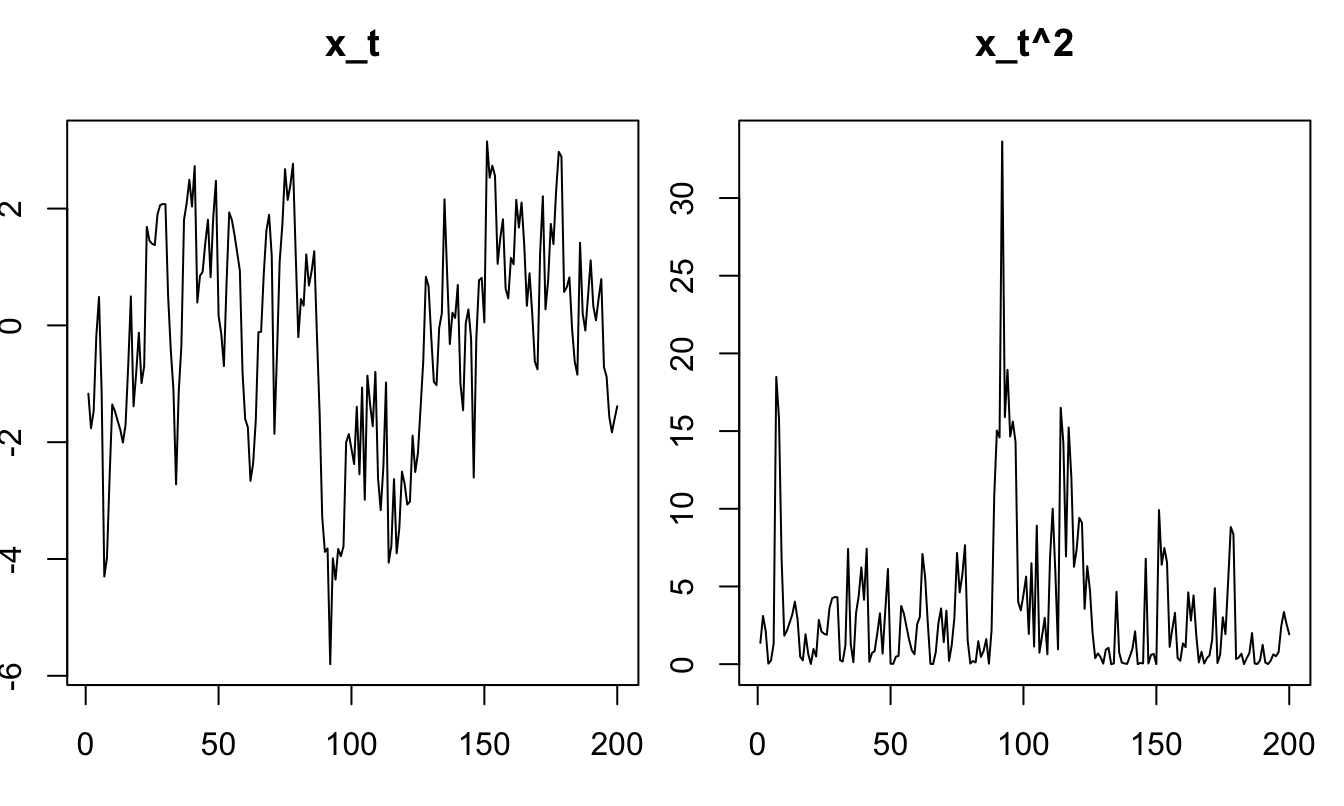
\includegraphics[width=0.95\linewidth]{TSM_files/figure-latex/simQVAR-1} \caption{Simulation of a quadratic processes $x_t$.}\label{fig:simQVAR}
\end{figure}

\end{example}

Another example of nonnegative process is that of the auto-regressive Gamma process \citep{Gourieroux_Jasiak_2006} and its extension \citep{zarg_2017}.

\begin{example}[Autoregressive gamma process, ARG(1)]
\protect\hypertarget{exm:ARG1}{}\label{exm:ARG1}

An ARG process is defined as follows:
\[
\frac{w_{t+1}}{\mu} \sim \gamma(\nu+z_t) \quad \mbox{where} \quad z_t \sim \mathcal{P} \left( \frac{\rho w_t}{\mu} \right),
\]
with \(\nu\), \(\mu\), \(\rho > 0\). (Alternatively \(z_t \sim {\mathcal{P}}(\beta w_t)\), with \(\rho = \beta \mu\).)

Proposition \ref{prp:LTARG} shows that we have \(\varphi_t(u) = \exp[a(u)'w_t+b(u)]\) with
\[
\left\{
\begin{array}{ccc}
a(u) &=&  \dfrac{\rho u}{1-u \mu}\\
b(u) &=& -\nu  
\log(1-u \mu).
\end{array}
\right.
\]

One can simulate ARG processes by using \href{https://jrenne.shinyapps.io/Affine/}{this web-interface} (select the ``ARG'' panel).

It can be shown that:
\[
\left\{
\begin{array}{ccc}
\mathbb{E}(w_{t+1}|\underline{w_t}) &=& \nu \mu + \rho w_t \\
\mathbb{V}ar(w_{t+1}|\underline{w_t}) &=& \nu \mu^2 + 2 \mu \rho w_t.
\end{array}
\right.
\]
and that:
\[
w_{t+1}=\nu\mu+\rho w_t+\varepsilon_{t+1},
\]
where \(\varepsilon_{t+1}\) is a martingale difference \(\Rightarrow\) \(w_{t+1}\) is a weak \(AR(1)\).

\citet{zarg_2017} porpose the extended ARG process and the ARG\(_0\) process. The latter is such that \(\nu = 0\) and \(\beta w_t\) is replaced with \(\alpha + \beta w_t\), i.e.:
\begin{equation}
\frac{w_{t+1}}{\mu} \sim \gamma(z_t),\quad z_t \sim {\mathcal{P}}(\alpha + \beta w_t).\label{eq:ARG0}
\end{equation}
It is easily seen that we then have:
\[
\varphi_t(u) = exp \left[\frac{\beta \mu u}{1-u \mu} w_t + \frac{\alpha \mu u}{1-u \mu}
\right].
\]
The ARG\(_0\) process features a point mass at zero, with conditional probability \(exp(-\alpha - \beta w_t)\). Note that 0 is absorbing if \(\alpha = 0\).

Figure \ref{fig:simARG0} displays the simulated path of an ARG\(_0\) process (since we set \(\nu\) to zero). Note that function \texttt{simul.ARG} is included in the \texttt{TSModels} package.

\begin{Shaded}
\begin{Highlighting}[]
\FunctionTok{library}\NormalTok{(TSModels)}
\NormalTok{W }\OtherTok{\textless{}{-}} \FunctionTok{simul.ARG}\NormalTok{(}\DecValTok{300}\NormalTok{,}\AttributeTok{mu=}\NormalTok{.}\DecValTok{5}\NormalTok{,}\AttributeTok{nu=}\DecValTok{0}\NormalTok{,}\AttributeTok{rho=}\NormalTok{.}\DecValTok{9}\NormalTok{,}\AttributeTok{alpha=}\NormalTok{.}\DecValTok{1}\NormalTok{)}
\FunctionTok{plot}\NormalTok{(W,}\AttributeTok{type=}\StringTok{"l"}\NormalTok{)}
\end{Highlighting}
\end{Shaded}

\begin{figure}
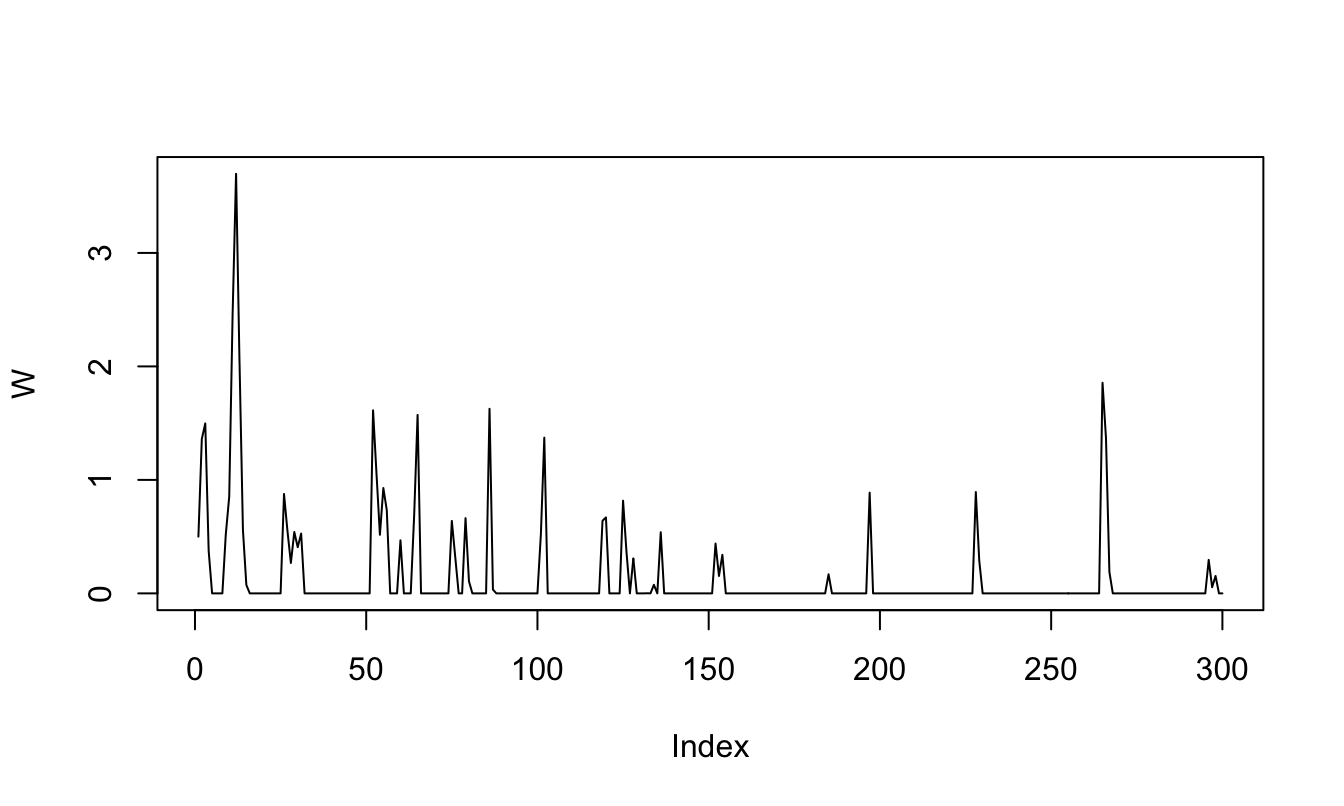
\includegraphics[width=0.95\linewidth]{TSM_files/figure-latex/simARG0-1} \caption{Simulation of an ARG0 processes.}\label{fig:simARG0}
\end{figure}

\end{example}

Certain affine processes are valued in specific sets (e.g., integers). It is the case of compound Poisson proceses:

\begin{example}[Compound Poisson process]
\protect\hypertarget{exm:CompoundPoisson}{}\label{exm:CompoundPoisson}

A compound Poisson process is defined as follows (with \(\gamma > 0\), \(0 < \pi< 1\), and \(\lambda > 0\)):
\[\frac{w_{t+1}}{\gamma} = z_{t+1} + \varepsilon_{t+1},
\]
where \(z_{t+1}\) and \(\varepsilon_{t+1}\) conditionally independent, and where
\(z_{t+1} \sim {\mathcal B} \left(\frac{w_t}{\gamma},\pi\right)\), with \(\varepsilon_{t+1} \sim {\mathcal P}(\lambda)\).

This process is valued in \(\{j \gamma, j \in \mathbb{N}, \gamma \in \mathbb{R}^+\}\) and we have:
\[
\varphi_t(u) = \exp\left\{
\begin{array}{l}
\dfrac{w_t}{\gamma}   \log[\pi
\exp(u\gamma)+1-\pi]-\lambda[1-\exp(u \gamma)]
\end{array}
\right\},
\]
i.e., \(\varphi_t(u) = \exp\left(a(u)w_t+b(u)\right)\) with
\[
\left\{
\begin{array}{ccl}
a(u)&=& \frac{1}{\gamma}   \log[\pi   \exp(u
\gamma)+1-\pi],\\
b(u) &=& -\lambda[1-\exp(u \gamma)].
\end{array}
\right.
\]

We also have: \(w_{t+1} = \pi w_t + \lambda \gamma + \eta_{t+1}\), where \(\eta_{t+1}\) is a
martingale difference.

One can simulate such processes by using \href{https://jrenne.shinyapps.io/Affine/}{this web-interface} (select the ``Compound Poisson'' panel). Figure \ref{fig:simCPoisson} makes use of function \texttt{simul.compound.poisson} (in package \texttt{TSModels}) to simulate a compound Poisson process.

\begin{Shaded}
\begin{Highlighting}[]
\FunctionTok{library}\NormalTok{(TSModels)}
\NormalTok{W }\OtherTok{\textless{}{-}} \FunctionTok{simul.compound.poisson}\NormalTok{(}\DecValTok{100}\NormalTok{,}\AttributeTok{Gamma=}\NormalTok{.}\DecValTok{5}\NormalTok{,}\AttributeTok{Pi=}\FloatTok{0.5}\NormalTok{,}\AttributeTok{lambda=}\NormalTok{.}\DecValTok{9}\NormalTok{)}
\FunctionTok{plot}\NormalTok{(W,}\AttributeTok{type=}\StringTok{"l"}\NormalTok{)}
\end{Highlighting}
\end{Shaded}

\begin{figure}
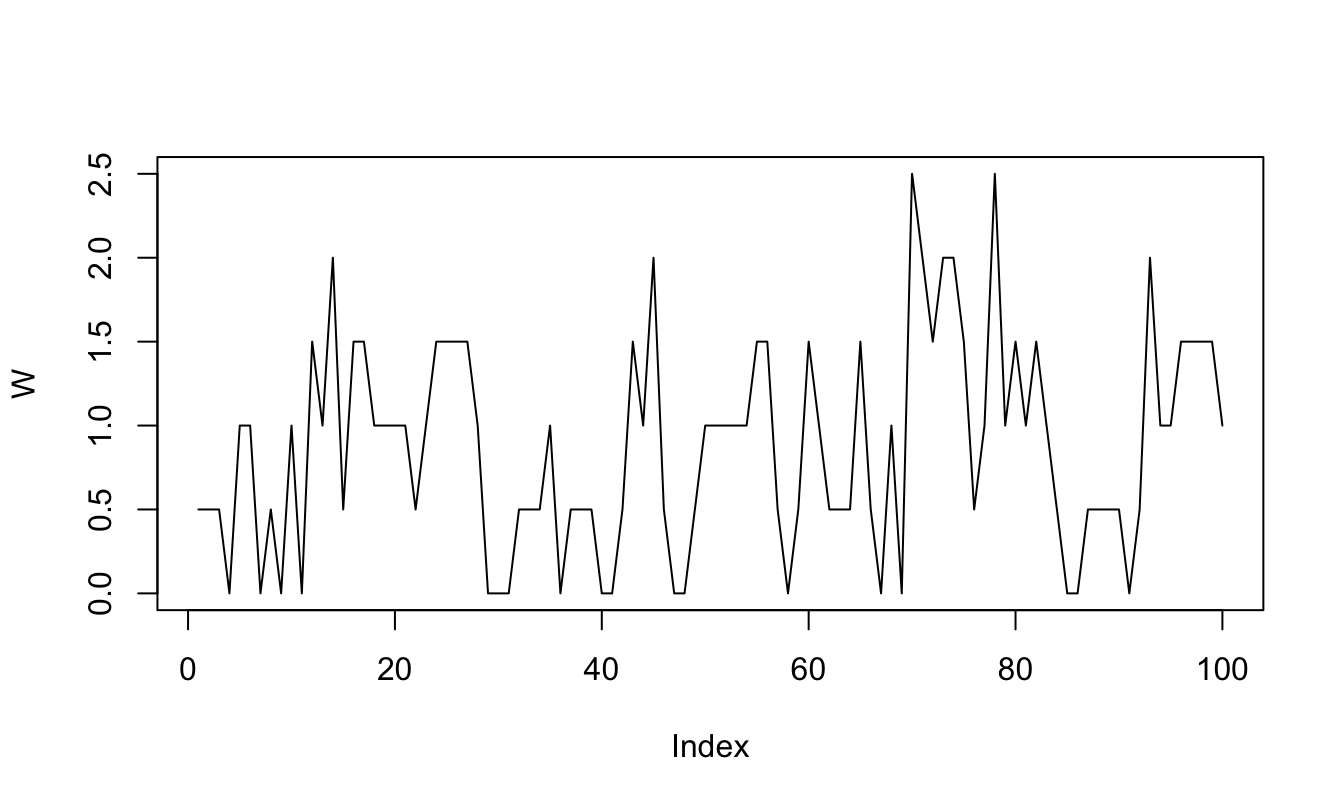
\includegraphics[width=0.95\linewidth]{TSM_files/figure-latex/simCPoisson-1} \caption{Simulation of a Compound Poisson process.}\label{fig:simCPoisson}
\end{figure}

\end{example}

\hypertarget{SubCarp}{%
\subsection{\texorpdfstring{Car processes of order \(p\)}{Car processes of order p}}\label{SubCarp}}

Let us now define Car processes of order \(p\):

\begin{definition}[Affine process of order p]
\protect\hypertarget{def:Carp}{}\label{def:Carp}A multivariate process \(w_{t+1}\) is affine of order \(p\) {[}or \(Car(p)\){]} if there exist functions \(a_1(.),\dots,a_p(.)\), and \(b(.)\) such that:
\[
\varphi_t(u)=\mathbb{E}_t[\exp(u' w_{t+1})]=\exp[a_1(u)'w_t+\dots+a_p(u)'w_{t+1-p}+b(u)].
\]
\end{definition}

It can be seen that if \(w_t\) is \(Car(p)\), then \(W_t = [w_t', w_{t-1}',\dots,w_{t-p+1}']'\) is \(Car(1)\).\footnote{We have:
  \begin{eqnarray*}
  \mathbb{E}_t[\exp(u'W_{t+1})] &=& \mathbb{E}_t[\exp(u'_1 w_{t+1}+u'_2 w_t+\dots+u'_p w_{t-p+2})] \\
  &=& \exp(u'_2 w_t+\dots+u'_p w_{t-p+2})\mathbb{E}_t[\exp(u'_1 w_{t+1})] \\
  &=& \exp(u'_2 w_t+\dots+u'_p w_{t-p+2}+a'_1(u_1)
  w_t  +\dots+a'_p(u_1)w_{t+1-p}+b(u_1)) \\
  &=& \exp[A(u)'W_t+B(u)],
  \end{eqnarray*}
  with \(A(u)' = [u'_2+a'_1(u_1),\dots,u'_p+a'_{p-1}(u_1), a'_p(u_1)]\) and \(B(u) = b(u_1)\).} Therefore, without loss of generality we can assume \(p = 1\).

The standard Car(\(p\)) processes are auto-regressive processes of order \(p\). These processes satisfy the definition of index affine processes:

\begin{definition}[Univariate index affine process of order p]
Let \(\exp[a(u)w_t+b(u)]\) be the conditional Laplace transform of a univariate affine process of order 1, the process \(w_{t+1}\) is an \emph{index-affine} process of order \(p\) if:
\[
\varphi_t(u)=\mathbb{E}_t[\exp(u w_{t+1})]=\exp[a(u)(\beta_1 w_t+\dots+\beta_p
w_{t+1-p})+b(u)].
\]
\end{definition}

Examples \ref{exm:ARp} and \ref{exm:ARGp} are two examples of index affine processes.

\begin{example}[Gaussian AR(p) process]
\protect\hypertarget{exm:ARp}{}\label{exm:ARp}This example extends Example \ref{exm:GAR1}. Consider a Gaussian AR(p) process \(w_t\); that is:
\[
w_{t+1} = \nu + \varphi_1 w_t +\dots+ \varphi_p w_{t+1-p}+\sigma \varepsilon_{t+1},\quad \varepsilon_{t+1} \sim i.i.d. \mathcal{N}(0,1).
\]
We have:
\[
\varphi_t(u) = \exp \left[ u \rho (\beta_1 w_t+\dots+\beta_p w_{t+1-p})+u\nu + u^2  \frac{\sigma^2}{2}\right]
\]
with \(\varphi_i = \rho \beta_i\).
\end{example}

\begin{example}[ARG(p) process (positive)]
\protect\hypertarget{exm:ARGp}{}\label{exm:ARGp}This example extends Example \ref{exm:ARG1}.
An ARG process of order \(p\) is defined as follows:
\[
\frac{w_{t+1}}{\mu} \sim \gamma(\nu+z_t) \quad \mbox{where} \quad z_t \sim \mathcal{P} \left( \beta_1 w_t+\dots+\beta_p w_{t+1-p} \right),
\]
with \(\nu\), \(\mu\), \(\beta_i > 0\). We have:
\[
\varphi_t(u) = \exp\left[\frac{\rho u}{1-u \mu} (\beta_1 w_t+\dots+\beta_p w_{t+1-p})-\nu  \log(1-u\mu)\right],
\]
Process \(w_t\) admits the following AR(\(p\)) representation:
\[
w_{t+1} = \nu\mu + \varphi_1 w_t +\dots+ \varphi_p w_{t+1-p}+\varepsilon_{t+1},
\]
with \(\varphi_i = \beta_i\mu\) and where \(\varepsilon_{t+1}\) is a martingale difference.
\end{example}

\hypertarget{Markov}{%
\section{Markov chains}\label{Markov}}

In this subsection, we show that the family of affine processes includes (some) regime-switching models. We consider a time-homogeneous Markov chain \(z_t\), valued in the set of columns of \(Id_J\), the identity matrix of dimension \(J \times J\). The transition probabilities are denoted by \(\pi(e_i, e_j)\), with \(\pi(e_i, e_j) = \mathbb{P}(z_{t+1}=e_j | z_t=e_i)\). With these notations:
\[
\mathbb{E}[\exp(v'z_{t+1})|z_t=e_i,\underline{z_{t-1}}] = \sum^J_{j=1} \exp(v'e_j)\pi (e_i, e_j).
\]
Hence, we have:
\[
\varphi_t(v) = \exp[a_z(v)'z_t],
\]
with
\[
a_z(v)= \left[ \begin{array}{c} \log \left(\sum^J_{j=1} \exp(v'e_j)  \pi(e_1,e_j)\right)\\
\vdots\\
\log \left(\sum^J_{j=1} \exp(v'e_j)  \pi(e_J,e_j)\right)
\end{array}\right].
\]
This proves that \(z_t\) is an affine process.

One can simulate a two-regime Markov chain by using \href{https://jrenne.shinyapps.io/Affine/}{this web-interface} (select the ``Markov-Switching'' panel).

\hypertarget{WAR}{%
\section{Wishart autoregressive (WAR) processes}\label{WAR}}

WAR are \emph{matrix processes}, valued in the space of \((L \times L)\) symmetric positive
definite matrices.

\begin{definition}[Wishart autoregressive (WAR) processes]
\protect\hypertarget{def:WAR}{}\label{def:WAR}Let \(W_{t+1}\) be a \(WAR_L(K, M, \Omega)\) process. It is defined by:
\begin{eqnarray}
&&\mathbb{E}[\exp   Tr(\Gamma W_{t+1})|\underline{W_t}] \label{eq:Trace}\\
&=& \exp\left\{Tr[M'\Gamma(Id-2\Omega \Gamma)^{-1}M W_t]  -  \frac{K}{2}   \log [det(Id-2\Omega \Gamma)]\right\}, \nonumber
\end{eqnarray}
where \(\Gamma\) is a symmetric matrix,\footnote{Indeed, \(Tr(\Gamma W_{t+1})\) is equal to:
  \(\sum^L_{i=1}(\Gamma W_{t+1})_{ii} = \sum^L_{i=1} \sum^L_{j=1} \gamma_{ij} W_{t+1,ij} = \sum^L_{i=1} \gamma_{ii} W_{t+1,ii} + \sum^L_{i<j} (\gamma_{ij}+\gamma_{ji}) W_{t+1,ij}\).} \(K\) is a positive scalar, \(M\) is a \((L \times L)\) matrix, and \(\Omega\) is a \((L \times L)\) symmetric positive definite matrix.
\end{definition}

If \(K\) is an integer, Proposition \ref{prp:WARAR} (in the appendix) shows that \(W_{t+1}\) can be obtained from:
\begin{eqnarray*}
\left\{
\begin{array}{ccl}
W_{t+1} & =&  \sum^K_{k=1} x_{k,t+1} x'_{k,t+1}\\
&&\\
x_{k,t+1} & =& M x_{k,t} + \varepsilon_{k,t+1},\quad k \in \{1,\dots,K\},
\end{array}
\right.
\end{eqnarray*}
where \(\varepsilon_{k,t+1} \sim i.i.d. \mathcal{N}(0, \Omega)\) (independent across \(k\)'s).
The proposition also shows that we have:
\[
\mathbb{E}(W_{t+1}|\underline{W_t}) = MW_tM'+K \Omega,
\]
i.e.~\(W_t\) follows a matrix weak AR(1) process.

In particular case, where \(L=1\) (univariate case), we have that:
\begin{eqnarray*}
\mathbb{E}[\exp(u W_{t+1})|\underline{W_t}] = \exp\left[
\frac{u m^2}{1-2\omega u}W_t -
\frac{K}{2}   \log(1-2\omega u)\right].
\end{eqnarray*}
Hence, when \(L=1\), the Wishart process boils down to an \(ARG(1)\) process (Example \ref{exm:ARG1}) with \(\rho = m^2\), \(\mu = 2\omega\), \(\nu = \frac{K}{2}\).

\hypertarget{building}{%
\section{Building affine processes}\label{building}}

\hypertarget{stoch}{%
\subsection{Univariate affine processes with stochastic parameters}\label{stoch}}

Some univariate affine processes can be extended if they satisfy certain conditions. Specifically, consider a univariate affine process whose conditional L.T. is of the form:
\begin{equation}
\mathbb{E}_t   \exp(u y_{t+1}) = \exp[a_0(u)y_t+b_0(u)\delta],\label{eq:extaffine}
\end{equation}
where \(\delta = (\delta_1,\dots,\delta_m)' \in \mathcal{D}\). This process can be generalized by making \(\delta\) stochastic (while staying in the affine family). More precisely assume that:
\[
\mathbb{E}[\exp(u y_{t+1})|\underline{y_t}, \underline{z_{t+1}}] = \exp[a_0(u)y_t+b_0(u)'\Lambda z_{t+1}],
\]
where \(\Lambda\) is a \((m\times k)\) matrix, with \(\Lambda z_{t+1} \in \mathcal{D}\). In this case, if:
\[
\mathbb{E}[\exp(v' z_{t+1})|\underline{y_t}, \underline{z_{t}}] = \exp[a_1(v)'z_t+b_1(v)],
\]
then \(w_{t+1} = (y_{t+1}, z'_{t+1})'\) is affine.\footnote{Indeed, we have:
  \begin{eqnarray*}
  &&\mathbb{E}[\exp(u y_{t+1}+v'z_{t+1})|\underline{y_t}, \underline{z_{t}}] \\
  &=& \mathbb{E}\{\exp(v' z_{t+1})\mathbb{E}[\exp(u y_{t+1})|\underline{y_t},
  \underline{z_{t+1}}]|\underline{y_t}, \underline{z_{t}} \} \\
  &=& \mathbb{E}\{\exp[a_0(u) y_{t}+b_0(u)'\Lambda z_{t+1}+v'z_{t+1}]|\underline{y_t},
  \underline{z_{t}} \} \\
  &=& \exp\{ a_0(u) y_{t}+a_1[\Lambda' b_0(u)+v]'z_t+b_1 [\Lambda' b_0(u)+v]\}.
  \end{eqnarray*}}

\begin{example}[Gaussian AR(p)]
\protect\hypertarget{exm:extendedARp}{}\label{exm:extendedARp}

Using the notation of Example \ref{exm:ARp}, it comes that an AR(p) processes satisfies Eq. \eqref{eq:extaffine} with \(b_0(u) = \left(u, \; \frac{u^2}{2}\right)'\) and \(\delta = (\nu,\sigma^2)' \in \mathcal{D}=\mathbb{R} \times \mathbb{R}^+\). In that case, \(\delta\) (the vector of conditional mean and variance) can be replaced by \ldots{}

\begin{itemize}
\tightlist
\item
  \(\left( \begin{array}{l} z_{1,t+1} \\ z_{2,t+1} \end{array} \right)\), where \(z_{1,t+1}\) and \(z_{2,t+1}\) are independent AR(1) (see Example \ref{exm:GAR1}) and ARG(1) (see Example \ref{exm:ARG1}) processes, respectively.
\item
  \(\left( \begin{array}{ll} \lambda'_1 & 0 \\ 0 & \lambda'_2 \end{array} \right)\)\(\left( \begin{array}{l} z_{1,t+1} \\ z_{2,t+1} \end{array} \right)\), where \(z_{1,t+1}\) and \(z_{2,t+1}\) are independent Markov chains.
\item
  \(\left( \begin{array}{l} \lambda'_1 \\ \lambda'_2 \end{array}\right)z_{t+1}\), where \(z_{t+1}\) is a Markov chain.
\end{itemize}

\end{example}

\begin{example}[ARG(p) model]
\protect\hypertarget{exm:ARGp}{}\label{exm:ARGp}\leavevmode

\begin{itemize}
\tightlist
\item
  \(b_0(u)= - \nu \log(1-u\mu)\), \(\delta=\nu\).
\item
  \(\nu\) (\(\ge 0\)) can be specified for instance as a Markov chain or an ARG.
\end{itemize}

\end{example}

\hypertarget{buildingmulti}{%
\subsection{Multivariate affine processes}\label{buildingmulti}}

One can construct multivariate affine processes by employing the so-called recursive approach. Let us illustrate this by considering the bivariate case. (The multivariate generalization is straightforward.) Consider \(w_t = \left(\begin{array}{c} w_{1,t}\\ w_{2,t} \end{array} \right)\),and assume that we have:
\begin{eqnarray*}
&&\mathbb{E}[\exp(u_1 w_{1,t+1}|\underline{w_{1,t}}, \underline{w_{2,t}})]\\
&=& \exp[a_{11}(u_1)w_{1,{\color{red}{t}}}+a_{12}(u_1)w_{2,{\color{red}{t}}}+b_{1}(u_1)],
\end{eqnarray*}
(which defines \(w_{1,t+1}|\underline{w_{1,t}}, \underline{w_{2,t}}\)) and:
\begin{eqnarray*}
&& \mathbb{E}[\exp(u_2 w_{2,t+1}|\underline{w_{1,t+1}}, \underline{w_{2,t}})]\\
&= & \exp[a_0(u_2)w_{1,{\color{red}{t+1}}}+a_{21}(u_2)w_{1,{\color{red}{t}}}+a_{22}(u_2)w_{2,{\color{red}{t}}}+b_2(u_2)]
\end{eqnarray*}
(which defines \(w_{2,t+1}|\underline{w_{1,t+1}}, \underline{w_{2,t}}\)). Then \(w_t\) is an affine process.\footnote{Indeed, we have:
  \begin{eqnarray*}
  && \mathbb{E}[\exp(u_1 w_{1,t+1}+u_2 w_{2,t+1}|\underline{w_{1,t}}, \underline{w_{2,t}})]\\
  &= & \mathbb{E}\{\exp(u_1 w_{1,t+1}) \mathbb{E}[\exp(u_{2}w_{2,t+1})|\underline{w_{1,t+1}}, \underline{w_{2,t}})]|\underline{w_{1,t}}, \underline{w_{2,t}})\} \\
  &= & \mathbb{E}\{\exp[u_1+a_0(u_2)w_{1,t+1}+a_{21}(u_2)w_{1,t} + a_{22}(u_2)w_{2,t}+b_2(u_2)]|\underline{w_{1,t}}, \underline{w_{2,t}})\} \\
  &= & \exp\{a_{11}[u_1+a_0(u_2)]w_{1,t}+a_{12}[u_1+a_0(u_2)]w_{2,t}+b_1[u_1+a_0(u_2)] \\
  &&+  a_{21}(u_2)w_{1,t}+a_{22}(u_2)w_{2,t}+b_2(u_2)\}.
  \end{eqnarray*}}
The dynamics of the two components of \(w_t\) are of the form:
\begin{eqnarray*}
w_{1,t+1} &=& \alpha_1 \hspace{1.55cm} + \alpha_{11}w_{1,t} + \alpha_{12}w_{2,t} + \varepsilon_{1,t+1} \\
w_{2,t+1} &=& \alpha_2 + \alpha_{0}w_{1,t+1} + \alpha_{21}w_{1,t} + \alpha _{22} w_{2,t} + \varepsilon_{2,t+1}
\end{eqnarray*}
Note that \(\varepsilon_{1,t+1}\) and \(\varepsilon_{2,t+1}\) are non-correlated martingale differences. In the general case, they are conditionally heteroskedastic. What precedes is at play in \(VAR\) model; \citet{zarg_2017} employ this approach to build vector auto-regressive gamma (VARG) processes.

\hypertarget{extending-multivariate-stochastic-processes}{%
\subsection{Extending multivariate stochastic processes}\label{extending-multivariate-stochastic-processes}}

Consider the same framework as in Section \ref{stoch} when \(y_t\) is a \(n\)-dimensional vector. That is, replace Eq. \eqref{eq:extaffine} with:
\begin{equation}
\mathbb{E}_t   \exp(u' y_{t+1}) = \exp[a_0(u)'y_t+b_0(u)\delta],\label{eq:Multiextaffine}
\end{equation}
and further assume that \(\delta\) is stochastic and depends on \(z_t\), such that:
\[
\mathbb{E}[\exp(u y_{t+1})|\underline{y_t}, \underline{z_{t+1}}] = \exp[a_0'(u)y_t+b_0(u)\Lambda z_{t+1}],
\]
where \(\Lambda\) is a \((m\times k)\) matrix, with \(\Lambda z_{t+1} \in \mathcal{D}\). In this case, if:
\[
\mathbb{E}[\exp(v' z_{t+1})|\underline{y_t}, \underline{z_{t}}] = \exp[a_1(v)'z_t+b_1(v)],
\]
then \(w_{t+1} = (y_{t+1}, z'_{t+1})'\) is affine.

\begin{example}[Stochastic parameters Gaussian VAR(1)]
\protect\hypertarget{exm:RSVAR}{}\label{exm:RSVAR}

This example extends Example \ref{exm:GVAR1}. Using the same notations as in the latter example \ref{exm:GVAR1}, we have
\[
b_0(u) = \left(u', \frac{1}{2} (u \otimes u)'\right)' \quad \mbox{and} \quad\delta = (\mu', vec(\Sigma)')' \in \mathbb{R}^n \times vec(\mathcal{S}),
\]
where \(\mathcal{S}\) is the set of symmetric positive semi-definite matrices. Vector \(\delta\) can be replaced by:
\[
\left( \begin{array}{l} z_{1,t+1}
\\ z_{2,t+1}
\end{array} \right),
\]
where

\begin{itemize}
\tightlist
\item
  \(z_{1,t+1}\) is, for instance, a Gaussian VAR process.
\item
  \(z_{2,t+1}\) is

  \begin{itemize}
  \tightlist
  \item
    obtained by applying the \(vec\) operator to a Wishart process,
  \item
    replaced by \(\Lambda_2 z_{2,t+1}\), where \(\Lambda_2\) is a \((n^2 \times J)\) matrix whose columns are \(vec(\Sigma_j)\), \(j \in \{1,\dots,J\}\), the \(\Sigma_j\) being \((n \times n)\) positive semi-definite, and \(z_{2,t+1}\) is a selection vector of dimension \(J \times 1\),
  \item
    a standardized \(J\)-dimensional VARG process (multivariate extension of Example \ref{exm:ARG1}).
  \end{itemize}
\end{itemize}

\end{example}

\begin{example}[Regime-switching VAR(1)]
\protect\hypertarget{exm:RSVAR2}{}\label{exm:RSVAR2}

One can also use this approach to construct (affine) regime-switching VAR processes (which is another extension of Example \ref{exm:GVAR1} (see, e.g., \citet{Gourieroux_Monfort_Pegoraro_Renne_2014}). For that, replace \(\delta\) with

\begin{itemize}
\tightlist
\item
  \(\left( \begin{array}{ll} \Lambda_1 & 0 \\ 0 & \Lambda_2 \end{array} \right)\)\(\left( \begin{array}{l} z_{1,t+1} \\ z_{2,t+1} \end{array} \right)\), where \(\Lambda_1\) is a \((n \times J_1)\) matrix and \(z_{1,t+1}\) is a Markov chain valued in the set of selection vectors of size \(J_1\) (see Subsection \ref{Markov}), \(\Lambda_2\) is the same matrix as in Example \ref{exm:RSVAR} and \(z_{2,t+1}\) is a Markov chain valued in the set of selection vectors of size \(J_2\).
\item
  or \(\left( \begin{array}{l} \Lambda_1 \\ \Lambda_2 \end{array}\right)z_{t+1}\), where \(\Lambda_1\) and\(\Lambda_2\) are the same matrices as above with \(J_1=J_2=J\), and \(z_{t+1}\) is a Markov chain valued in the set of selection vectors of size \(J\).
\end{itemize}

\end{example}

\hypertarget{AffineExtended}{%
\subsection{Extended affine processes}\label{AffineExtended}}

Some processes are not affine, but may be sub-components of an affine process. This can be useful to compute their conditional moments and multi-horizon Laplace transform (as one can use the formulas presented above for that, using the enlarged---affine---vector).

Let us formally define an extended affine process:

\begin{definition}[Extended Affine Processes]
\protect\hypertarget{def:ExtAffine}{}\label{def:ExtAffine}A process \(w_{1,t}\) is extended affine if there exists a process \(w_{2,t} = g(\underline{w_{1,t}})\) such that \((w'_{1,t}, w'_{2,t})'\) is affine (of order 1).
\end{definition}

For an extended affine processes, \(\varphi_{1,t}(u) = \mathbb{E}[\exp(u'w_{1,t+1})|\underline{w_{1,t}}]\) can be obtained from:
\begin{eqnarray*}
\varphi_t(u_1, u_2) &=& \mathbb{E}[\exp(u'_1w_{1,t+1}+u'_2 w_{2,t+1)}|\underline{w_{1,t}}, \underline{w_{2,t}}] \\
&=& \exp[a'_1(u_1,u_2)w_{1,t} + a'_2(u_1,u_2)w_{2,t}+b(u_1,u_2)]
\end{eqnarray*}
by:
\[
\varphi_{1,t}(u) = \varphi_t(u, 0) = \exp[a'_1(u,0)w_{1,t}+a'_2(u,0)g(\underline{w_{1,t}}) + b(u, 0)].
\]
In particular \(w_{1,t}\) may be non-Markovian.

Similarly the multi-horizon Laplace transform (see Section \ref{MHLT})
\[
\mathbb{E}[\exp(\gamma'_{1}w_{1,t+1}+\dots+\gamma'_{h}w_{1,t+h})|\underline{w_{1,t}}]
\]
can be obtained from the knowledge of the extended multi-horizon Laplace transform:
\begin{eqnarray*}
&&\mathbb{E}_t[\exp(\{\gamma'_{1,1}w_{1,t+1}+\gamma'_{2,1}w_{2,t+1}\}+\dots+ \{\gamma'_{1,h}w_{1,t+h}+\gamma'_{2,h}w_{2,t+h}\}] \\
&=& \exp[A'_{1,t,h}(\gamma^h_1, \gamma^h_2)w_{1,t}+A'_{2,t,h}(\gamma^h_1, \gamma^h_2)w_{2,t}+B_{t,h}(\gamma^h_1, \gamma^h_2)],
\end{eqnarray*}
(with \(\gamma^h_1 = (\gamma'_{1,1},\dots, \gamma'_{1,h})'\), and \(\gamma^h_2 = (\gamma'_{2,1},\dots, \gamma'_{2,h})'\)). We indeed have:
\begin{eqnarray*}
&& \mathbb{E}[\exp(\gamma'_{1}w_{1,t+1}+\dots+\gamma'_{h}w_{1,t+h})|\underline{w_{1,t}}]\\
&=& \exp[A'_{1,t,h}(\gamma^h,0) w_{1,t} + A'_{2,t,h}(\gamma^h,0)g (\underline{w_{1,t}}) + B_{t,h}(\gamma^h,0)],
\end{eqnarray*}
with \(\gamma^h = (\gamma_1',\dots,\gamma_h')'\).

\begin{example}[Affine process of order p]
\protect\hypertarget{exm:AffProcessOrderp}{}\label{exm:AffProcessOrderp}If \(\{w_{1,t}\}\) is affine or order \(p>1\), then \((w_{1,t},\dots,w_{1,t-p+1})\) is affine of order 1, but \(\{w_{1,t}\}\) is not affine. That is, in that case, \(w_{2,t} = (w'_{1,t-1}, \dots.w'_{1,t-p+1})'\).

This a kind of extreme case since \(w_{2,t}\) belongs to the information at \(t-1\), which implies \(a_2(u_1, u_2) = u_2\).
\end{example}

\begin{example}[Gaussian ARMA process]
\protect\hypertarget{exm:GaussianARMA}{}\label{exm:GaussianARMA}Consider an \(ARMA(1,1)\) process
\[
w_{1,t} - \varphi w_{1,t-1} = \varepsilon_t-\theta \varepsilon_{t-1},
\]
with \(|\varphi | < 1\), \(|\theta| < 1\), and \(\varepsilon_t \sim i.i.d. \mathcal{N}(0, \sigma^2)\).

\(w_{1,t}\) is not Markovian. Now, take \(w_{2,t} = \varepsilon_t = (1-\theta L)^{-1}(1-\varphi L)w_{1,t}\). We have:
\[
\left(
\begin{array}{l}
w_{1,t+1} \\
w_{2,t+1}
\end{array}
\right) =
\left(
\begin{array}{ll}
\varphi & -\theta \\
0 &      0
\end{array}
\right)
\left(
\begin{array}{l}
w_{1,t} \\
w_{2,t}
\end{array}
\right) +
\left(
\begin{array}{l}
1 \\
1
\end{array}
\right) \varepsilon_{t+1}.
\]
Hence \((w_{1,t}, w_{2,t})'\) is Gaussian \(VAR(1)\), and, therefore, it is affine of order 1.

This is easily extended to \(ARMA(p,q)\) and \(VARMA(p,q)\) processes.
\end{example}

\begin{example}[GARCH type process]
\protect\hypertarget{exm:GARCH}{}\label{exm:GARCH}Consider process \(w_{1,t}\), defined by:
\[
w_{1,t+1}  = \mu + \varphi w_{1,t} + \sigma_{t+1} \varepsilon_{t+1},
\]
where \(|\varphi| < 1\) and \(\varepsilon_t \sim i.i.d. \mathcal{N}(0,1)\), and
\[
\sigma^2_{t+1} = \omega + \alpha \varepsilon^2_t + \beta \sigma^2_t,
\]
where \(0 < \beta < 1\).

Consider \(w_{2,t} = \sigma^2_{t+1}\) (which is a non-linear function of \(\underline{w_{1,t}}\)). Proposition \ref{prp:GARCH} shows that:
\begin{eqnarray*}
&& \mathbb{E}\left[\exp(u_1 w_{1,t+1} + u_2 w_{2,t+1})|\underline{w_{1,t}}\right] \\
&=& \exp\left[u_1 \mu + u_2 \omega - \frac{1}{2}   \log(1-2 u_2 \alpha) \right. \\
&&\left. +  u_1 \varphi w_{1,t} + (u_2\beta +  \frac{u^2_1}{2(1-2u_2\alpha)}) w_{2,t}\right],
\end{eqnarray*}
which is exponential affine in \((w_{1,t}, w_{2,t})\).
\end{example}

\hypertarget{MHLT}{%
\section{Multi-horizon Laplace transform}\label{MHLT}}

\hypertarget{recursive-computation-and-direct-pricing-implications}{%
\subsection{Recursive computation and direct pricing implications}\label{recursive-computation-and-direct-pricing-implications}}

In this subsection, we show that multi-horizon Laplace transforms of affine processes can be calculated recursively. Various examples will show how this can be exploited to price long-dated financial instruments.

Let us consider a multivariate process \(w_{t}\), affine of order one. (As explained in Subsection \ref{SubCarp}, this includes the case of the order \(p\) case.) For the sake of generality, we consider the case where functions \(a(.)\), \(b(.)\) are possibly deterministic functions of time, denoted in this case \(a_{t+1}(.)\) and \(b_{t+1}(.)\):
\[
\mathbb{E}_t \exp[(u'w_{t+1})] = \exp[a'_{t+1}(u)w_t+b_{t+1}(u)].
\]
The multi-horizon Laplace transform of associated with date \(t\) and horizon \(h\) is defined by:
\begin{equation}
\varphi_{t,h}(\gamma_1,\dots,\gamma_h) = \mathbb{E}_t[\exp(\gamma'_1w_{t+1}+\dots+\gamma'_h w_{t+h})].\label{eq:multiLT}
\end{equation}

Lemma \ref{lem:MHLT} (in the appendix) shows that we have:
\[
\varphi_{t,h}(\gamma_1,\dots,\gamma_h) = \exp(A'_{t,h} w_t + B_{t,h}),
\]
where \(A_{t,h} = A^h_{t,h}\) and \(B_{t,h} = B^h_{t,h}\), the \(A^h_{t,i}, B^h_{t,i}\) \(i = 1,\dots,h\), being given recursively by:
\[
\left\{
\begin{array}{ccl}
A^h_{t,i} &=& a_{t+h+1-i}(\gamma_{h+1-i} + A^h_{t,i-1}), \\
B^h_{t,i} &=& b_{t+h+1-i}(\gamma_{h+1-i} + A^h_{t,i-1}) + B^h_{t,i-1}, \\
A^h_{t,0} &=& 0, B^h_{t,0} = 0.
\end{array}
\right.
\]

If the functions \(a_{t}\) and \(b_{t}\) do not depend on \(t\), these recursive formulas do not depend on \(t\), and we get \(\varphi_{t,h}(\gamma_1,\dots,\gamma_h)\), for any \(t\), with only one recursion for each \(h\).

Moreover, if the functions \(a_{t}\) and \(b_{t}\) do not depend on \(t\), and if different sequences \((\gamma^h_1,\dots,\gamma^h_h), h=1,\dots,H\) (say) satisfy \(\gamma^h_{h+1-i} = u_i\), for
\(i=1,\dots,h\), and for any \(h \leq H\), that is if we want to compute (\emph{reverse-order} case):
\begin{equation}
\varphi_{t,h}(u_h,\dots,u_1)=\mathbb{E}_t[\exp(u'_{{\color{red}h}} w_{{\color{red}t+1}}+\dots+u'_{{\color{red}1}} w_{{\color{red}t+h}})],
\quad h=1,\dots,H,\label{eq:LTreverse}
\end{equation}
then Proposition \ref{prp:reverseMLT} (in the appendix) shows that we can compute the \(\varphi_{t,h}(u_h,\dots,u_1)\) for any \(t\) and any \(h \leq H\) with only one recursion. That is \(\varphi_{t,h}(u_h,\dots,u_1)=\exp(A'_hw_t+B_h)\) with:
\begin{equation*}
\left\{
\begin{array}{ccl}
A_{h} &=& a(u_{h} + A_{h-1}), \\
B_{h} &=& b(u_{h} + A_{h-1}) + B_{h-1}, \\
A_{0} &=& 0,\quad  B_{0} = 0.
\end{array}
\right.
\end{equation*}

As mentioned above, what precedes has useful implications to price long-dated financial instruments such as nominal and real bonds (Examples \ref{exm:nominalBth} and \ref{exm:realBth}, respectively), or futures (Example \ref{exm:Futures}).

\begin{example}[Nominal interest rates]
\protect\hypertarget{exm:nominalBth}{}\label{exm:nominalBth}Let \(B(t,h)\) denote the date-\(t\) price of a nominal zero-coupon bond of maturity \(h\). We Have:
\begin{equation}
B(t,h) = \mathbb{E}^{\mathbb{Q}}_t \exp (-r_{t}-\dots-r_{t+h-1}),\label{eq:stdbond}
\end{equation}
where \(r_{t}\) is the nominal short rate between \(t\) and \(t+1\) (observed at \(t\)), and the associated (continuously-compounded) yield-to-maturity is given by:
\begin{equation}
R(t,h) = -  \frac{1}{h}   \log   B(t,h), \quad   h=1,\dots,H.
\end{equation}
If \(r_t = \omega'w_t\) (say), then:
\[
B(t,h) = \exp(-r_{t}) \mathbb{E}^{\mathbb{Q}}_t \exp(-\omega' w_{t+1} - \dots - \omega' w_{t+h-1}).
\]
One can then price this bond by directly employing Eq. \eqref{eq:LTreverse}, with \(u_1 = 0\) and \(u_i = - \omega\), \(i = 2,\dots, H\).
The price \(B(t,h)\) is exponential affine in \(w_t\), the associated yield-to-maturity \(R(t,h)=-1/h\log B(t,h)\) is affine in \(w_t\).
\end{example}

\begin{example}[No-arbitrage Nelson-Siegel model]
\protect\hypertarget{exm:CDR2009}{}\label{exm:CDR2009}

In this example, we employ the results of Example \ref{exm:nominalBth} in the context described by \citet{Christensen_Diebold_Rudebusch_2009}. Specifically, we consider a three factor model following a Gaussian VAR (see Example \ref{exm:GVAR1}):
\[
w_t = \left[\begin{array}{c}X_{1,t}\\X_{2,t}\\X_{3,t}\end{array}\right] = 
\left[\begin{array}{ccc}
1 & 0 & 0\\
0&1-\lambda&\lambda\\
0&0&1-\lambda\end{array}\right]
\left[\begin{array}{c}X_{1,t-1}\\X_{2,t-1}\\X_{2,t-1}\end{array}\right] +
\left[\begin{array}{ccc}
\sigma_{11} & 0 & 0\\
\sigma_{21}&\sigma_{22}&0\\
\sigma_{31}&\sigma_{32}&\sigma_{33}\end{array}\right]
\left[\begin{array}{c}\varepsilon_{1,t}\\\varepsilon_{2,t}\\\varepsilon_{3,t}\end{array}\right],
\]
where \(\left[\begin{array}{c}\varepsilon_{1,t}\\\varepsilon_{2,t}\\\varepsilon_{3,t}\end{array}\right] \sim \,i.i.d.\, \mathcal{N}(0,Id)\).

The nominal short-term rate is given by \(r_t = X_{1,t}+X_{2,t}\). In that case, we can use the results of Example \ref{exm:nominalBth} with \(\omega = (-1,-1,0)'\). The following lines of code do that:

\begin{Shaded}
\begin{Highlighting}[]
\FunctionTok{library}\NormalTok{(TSModels)}
\NormalTok{lambda }\OtherTok{\textless{}{-}}\NormalTok{ .}\DecValTok{05}
\NormalTok{Phi }\OtherTok{\textless{}{-}} \FunctionTok{diag}\NormalTok{(}\FunctionTok{c}\NormalTok{(}\DecValTok{1}\NormalTok{,}\DecValTok{1}\SpecialCharTok{{-}}\NormalTok{lambda,}\DecValTok{1}\SpecialCharTok{{-}}\NormalTok{lambda));Phi[}\DecValTok{2}\NormalTok{,}\DecValTok{3}\NormalTok{] }\OtherTok{\textless{}{-}}\NormalTok{ lambda}
\NormalTok{Sigma }\OtherTok{\textless{}{-}}\NormalTok{ .}\DecValTok{0005} \SpecialCharTok{*} \FunctionTok{diag}\NormalTok{(}\DecValTok{3}\NormalTok{)}
\NormalTok{psi.parameterization}\OtherTok{=}\FunctionTok{list}\NormalTok{(}\AttributeTok{mu=}\FunctionTok{matrix}\NormalTok{(}\DecValTok{0}\NormalTok{,}\DecValTok{3}\NormalTok{,}\DecValTok{1}\NormalTok{),}\AttributeTok{Phi=}\NormalTok{Phi,}\AttributeTok{Sigma=}\NormalTok{Sigma)}
\NormalTok{u1 }\OtherTok{\textless{}{-}} \FunctionTok{matrix}\NormalTok{(}\DecValTok{0}\NormalTok{,}\DecValTok{3}\NormalTok{,}\DecValTok{1}\NormalTok{)}
\NormalTok{u2 }\OtherTok{\textless{}{-}} \FunctionTok{matrix}\NormalTok{(}\FunctionTok{c}\NormalTok{(}\SpecialCharTok{{-}}\DecValTok{1}\NormalTok{,}\SpecialCharTok{{-}}\DecValTok{1}\NormalTok{,}\DecValTok{0}\NormalTok{),}\AttributeTok{ncol=}\DecValTok{1}\NormalTok{)}
\NormalTok{H }\OtherTok{\textless{}{-}} \DecValTok{20}
\NormalTok{AB }\OtherTok{\textless{}{-}} \FunctionTok{reverse.MHLT}\NormalTok{(psi.GaussianVAR,}\AttributeTok{u1 =}\NormalTok{ u1,}\AttributeTok{u2 =}\NormalTok{ u2,}\AttributeTok{H =}\NormalTok{ H,}
                   \AttributeTok{psi.parameterization =}\NormalTok{ psi.parameterization)}
\NormalTok{AB}\SpecialCharTok{$}\NormalTok{A[}\DecValTok{1}\SpecialCharTok{:}\DecValTok{2}\NormalTok{,,] }\OtherTok{\textless{}{-}}\NormalTok{ AB}\SpecialCharTok{$}\NormalTok{A[}\DecValTok{1}\SpecialCharTok{:}\DecValTok{2}\NormalTok{,,] }\SpecialCharTok{{-}} \DecValTok{1} \CommentTok{\# add terms corresponding to exp({-}r\_t)}
\NormalTok{a.yield }\OtherTok{\textless{}{-}} \SpecialCharTok{{-}}\NormalTok{ AB}\SpecialCharTok{$}\NormalTok{A }\SpecialCharTok{/} \FunctionTok{array}\NormalTok{((}\DecValTok{1}\SpecialCharTok{:}\NormalTok{H) }\SpecialCharTok{\%x\%} \FunctionTok{rep}\NormalTok{(}\DecValTok{1}\NormalTok{,}\DecValTok{3}\NormalTok{),}\FunctionTok{c}\NormalTok{(}\DecValTok{3}\NormalTok{,}\DecValTok{1}\NormalTok{,H))}
\NormalTok{b.yield }\OtherTok{\textless{}{-}} \SpecialCharTok{{-}}\NormalTok{ AB}\SpecialCharTok{$}\NormalTok{B }\SpecialCharTok{/} \FunctionTok{array}\NormalTok{((}\DecValTok{1}\SpecialCharTok{:}\NormalTok{H) }\SpecialCharTok{\%x\%} \FunctionTok{rep}\NormalTok{(}\DecValTok{1}\NormalTok{,}\DecValTok{3}\NormalTok{),}\FunctionTok{c}\NormalTok{(}\DecValTok{1}\NormalTok{,}\DecValTok{1}\NormalTok{,H))}
\FunctionTok{plot}\NormalTok{(a.yield[}\DecValTok{1}\NormalTok{,,],}\AttributeTok{type=}\StringTok{"l"}\NormalTok{,}\AttributeTok{lwd=}\DecValTok{2}\NormalTok{,}\AttributeTok{ylim=}\FunctionTok{c}\NormalTok{(}\DecValTok{0}\NormalTok{,}\DecValTok{1}\NormalTok{),}
     \AttributeTok{xlab=}\StringTok{"Maturity"}\NormalTok{,}\AttributeTok{ylab=}\StringTok{"Factor loadings"}\NormalTok{)}
\FunctionTok{lines}\NormalTok{(a.yield[}\DecValTok{2}\NormalTok{,,],}\AttributeTok{col=}\StringTok{"red"}\NormalTok{,}\AttributeTok{lwd=}\DecValTok{2}\NormalTok{,}\AttributeTok{lty=}\DecValTok{2}\NormalTok{)}
\FunctionTok{lines}\NormalTok{(a.yield[}\DecValTok{3}\NormalTok{,,],}\AttributeTok{col=}\StringTok{"blue"}\NormalTok{,}\AttributeTok{lwd=}\DecValTok{2}\NormalTok{,}\AttributeTok{lty=}\DecValTok{3}\NormalTok{)}
\end{Highlighting}
\end{Shaded}

\begin{figure}
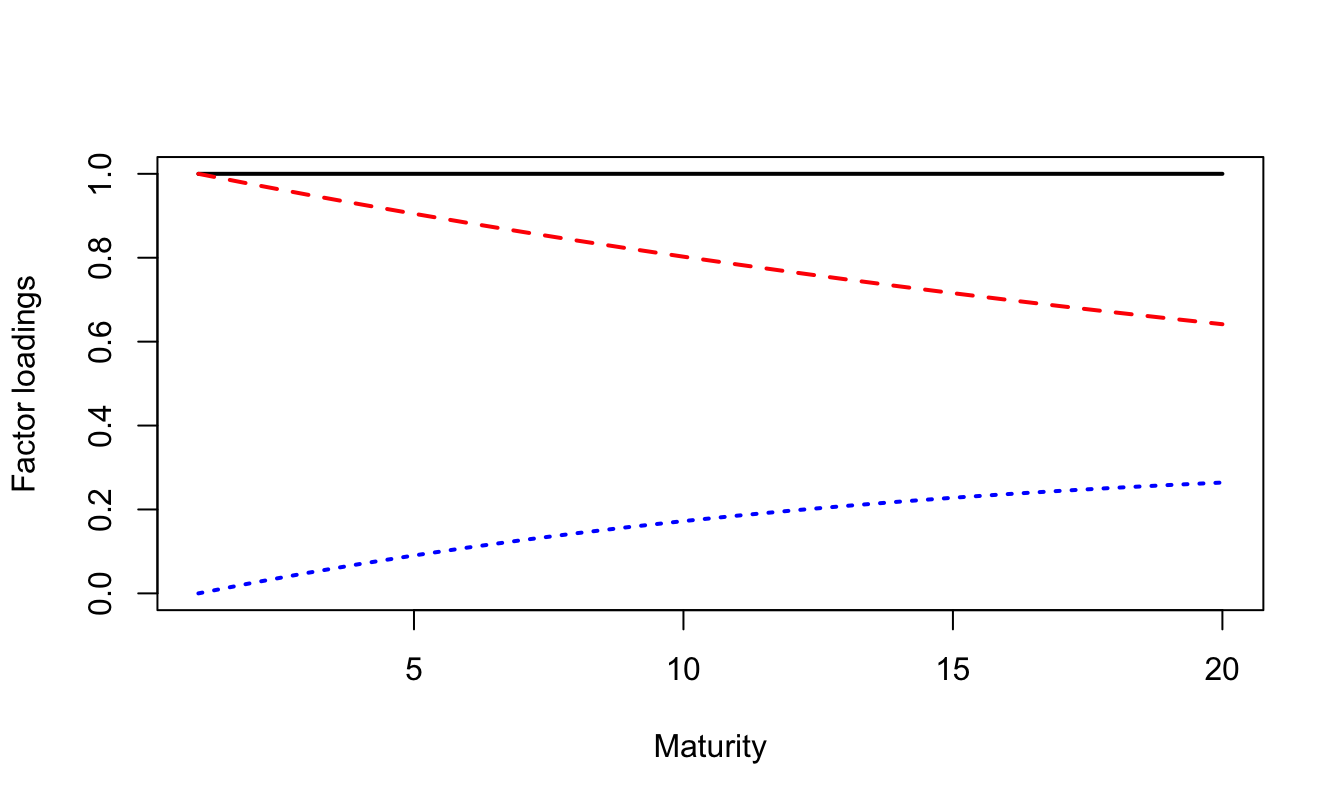
\includegraphics[width=0.95\linewidth]{TSM_files/figure-latex/CDR-1} \caption{Factor loadings in the context of a no-arbitrage nelson-Siegel model (Christensen, Diebold and Rudebusch, 2009). The first factor (black solid line) is a level factor. The second and third factors (red dashed line and blue dotted line, respectively) are slope factors.}\label{fig:CDR}
\end{figure}

\end{example}

In the previous example, note the use of function \texttt{reverse.MHLT} (in package \texttt{TSModels}), that notably takes a L.T. as an argument (\texttt{psi}). In the previous example, we consider a Gaussian VAR, and we therefore assign \texttt{psi.GaussianVAR} to \texttt{psi}. We then need to provide function \texttt{reverse.MHLT} with the arguments of the \texttt{psi} function. These arguments are provided in the form of a list (input \texttt{psi.parameterization}).

\begin{example}[Real interest rates]
\protect\hypertarget{exm:realBth}{}\label{exm:realBth}Denote by \(q_t\) the price index on date \(t\) and by \(\pi_{t+1} = \log \dfrac{q_{t+1}}{q_t}\) the inflation rate on date \(t+1\). We have:
\begin{eqnarray*}
\bar{R}(t,h) & =& -   \frac{1}{h}   \log   \bar{B}(t,h), \quad h=1,\dots,H \\    \\
\bar{B}(t,h) & =&  \mathbb{E}^{\mathbb{Q}}_t   \exp(-r_{t}-\dots-r_{t+h-1} + \pi_{t+1}+\dots+\pi_{t+h}),  \\      \\
& =& \exp(-r_{t}) \times \\
&& \mathbb{E}^{\mathbb{Q}}_t \exp(-r_{t+1}-\dots-r_{t+h-1}+\pi_{t+1}+\dots+\pi_{t+h})
\end{eqnarray*}
If \(r_t = \omega'w_t\) and \(\pi_t = \bar\omega'w_t\), then \(\bar{B}(t,h)\) is given by:
\begin{eqnarray*}
\exp(-r_{t}) \mathbb{E}^{\mathbb{Q}}_t \exp[(\bar\omega-\omega)'w_{t+1}+\dots+(\bar\omega-\omega)'w_{t+h-1}+\bar\omega'
w_{t+h}]
\end{eqnarray*}
One can then price this bond by directly employing Eq. \eqref{eq:LTreverse}, with \(u_1 = \bar\omega\) and \(u_i = \bar\omega-\omega\), \(i = 2,\dots, H\).
\end{example}

\begin{example}[Futures]
\protect\hypertarget{exm:Futures}{}\label{exm:Futures}

Denote by \(F(t,h)\) the date-\(t\) price of a future of maturity \(h\) (see Section XXX). That is \(F(t,h) = \mathbb{E}^{\mathbb{Q}}_t (S_{t+h})\), \(h=1,\dots,H\), where \(S_t\) is the date-\(t\) price of the underlying asset.

\begin{itemize}
\item
  If \(w_t = (\log S_t, x'_t)'\) then \(F(t,h) = \mathbb{E}^{\mathbb{Q}}_t \exp(e'_1 w_{t+h})\). This can be calculated by using Eq. \eqref{eq:LTreverse} with \(u_1 = e_1\), and \(u_i = 0\), for \(i=2,\dots,H\).
\item
  If \(w_t = (y_t, x'_t)'\) with \(y_t = \log\frac{S_t}{S_{t-1}}\), then \(F(t,h) = S_t \mathbb{E}^{\mathbb{Q}}_t \exp(e'_1 w_{t+1}+\dots+e'_1 w_{t+h})\). This can be calculated by using Eq. \eqref{eq:LTreverse} with \(u_i = e'_1\), \(i=1,\dots,H\).
\end{itemize}

\end{example}

\hypertarget{ExponentialPayoff}{%
\subsection{Exponential payoff}\label{ExponentialPayoff}}

Consider an asset providing the payoff \(\exp(\nu' w_{t+h})\) on date \(t+h\). Its price is given by:
\[
P(t,h;\nu) = \mathbb{E}^{\mathbb{Q}}_t[\exp(-r_{t}-\dots-r_{t+h-1}) \exp(\nu' w_{t+h})].
\]
If \(r_t = \omega'w_t\), we have:
\[
P(t,h;\nu) = \exp(-r_{t})\mathbb{E}^{\mathbb{Q}}_t \left(\exp[-\omega' w_{t+1}-\dots-\omega' w_{t+h-1}+ \nu' w_{t+h}]\right),
\]
which can be calculated by Eq. \eqref{eq:LTreverse}, with \(u_1 = \nu\) and \(u_i = -\omega\) for \(i = 2,\dots,H\).

What precedes can be extended to the case where the payoff (settled on date \(t+h\)) is of the form:
\[
(\nu_1'w_{t+h}) \exp(\nu_2' w_{t+h}).
\]
Indeed, we have
\[
\left[\frac{\partial \exp[(s \nu_1+ \nu_2)'w_{t+h}]}{\partial s}\right]_{s=0} = (\nu_1'w_{t+h}) \exp(\nu_2' w_{t+h}).
\]
Therefore:
\begin{eqnarray}
&&\mathbb{E}_t^{\mathbb{Q}}[\exp(-r_t - \dots - r_{t+h-1})(\nu_1'w_{t+h}) \exp(\nu_2' w_{t+h})] \nonumber\\
&=& \left[
\frac{\partial P(t,h;s \nu_1 + \nu_2)}{\partial s}
\right]_{s=0}.\label{eq:Affineexppayoff}
\end{eqnarray}
This method is easily extended to price payoffs of the form \((\nu_1'w_{t+h})^k \exp(\nu_2' w_{t+h})\), with \(k \in \mathbb{N}\).

\hypertarget{var-representation-and-conditional-moments}{%
\section{VAR representation and conditional moments}\label{var-representation-and-conditional-moments}}

An important property of affine processes is that their dynamics can be written as a vector-autoregressive process. This is useful to compute conditional moments of the process.

\begin{proposition}[VAR representation of an affine process' dynamics]
\protect\hypertarget{prp:affineVAR}{}\label{prp:affineVAR}If \(w_t\) is the affine process whose Laplace transform is defined in Def. \ref{def:Car1}, then its dynamics admits the following vectorial autoregressive representation:
\begin{equation}
w_{t+1} = \mu + \Phi w_{t} + \Sigma^{\frac{1}{2}}(w_t) \varepsilon_{t+1},\label{eq:VARw}
\end{equation}
where \(\varepsilon_{t+1}\) is a difference of martingale sequence whose conditional covariance matrix is the identity matrix and where \(\mu\), \(\Phi\) and \(\Sigma(w_t) = \Sigma^{\frac{1}{2}}(w_t){\Sigma^{\frac{1}{2}}(w_t)}'\) satisfy:
\begin{equation}
\mu =  \left[\frac{\partial }{\partial u}b(u)\right]_{u=0}, \quad \Phi= \left[\frac{\partial }{\partial u}a(u)'\right]_{u=0}\label{eq:MUPHI}
\end{equation}
\begin{equation}
\Sigma(w_t) =  \left[\frac{\partial }{\partial u\partial u'}b(u)\right]_{u=0} + \left[\frac{\partial }{\partial u\partial u'}a(u)'w_t\right]_{u=0}.\label{eq:SigmaWt}
\end{equation}
\end{proposition}

\begin{proof}
When \(w_t\) is affine, its (conditional) cumulant generating function is of the form \(\psi(u)=a(u)'w_t+b(u)\). The result directly follows from the formulas given in Section \ref{AffineLaplace}.
\end{proof}

Proposition \ref{prp:condvarAffine} (in the appendix) shows that the conditional means and variances of \(w_t\) are given by:
\begin{eqnarray}
\mathbb{E}_t(w_{t+h}) &=& (I - \Phi)^{-1}(I - \Phi^h)\mu + \Phi^h w_t \label{eq:condmean}\\
\mathbb{V}ar_t(w_{t+h}) &=& \Sigma(\mathbb{E}_t(w_{t+h-1}))+\Phi \Sigma(\mathbb{E}_t(w_{t+h-2}))\Phi' + \nonumber \\
&& \dots + \Phi^{h-1} \Sigma(w_{t}){\Phi^{h-1}}'. \label{eq:condvar}
\end{eqnarray}
Eq. \eqref{eq:condvar} notably implies that \(\mathbb{V}ar_t(w_{t+h})\) is an affine function of \(w_t\). Indeed \(\Sigma(.)\) is an affine function, and the conditional expectations \(\mathbb{E}_t(w_{t+h})\) are affine in \(w_t\), as shown by Eq. \eqref{eq:condmean}.

The unconditional means and variances are given by:
\begin{equation}
\left\{
\begin{array}{ccl}
\mathbb{E}(w_t) &=& (I - \Phi)^{-1}\mu\\
vec[\mathbb{V}ar(w_t)] &=& (I_{n^2} - \Phi \otimes \Phi)^{-1} vec\left(\Sigma[(I - \Phi)^{-1}\mu]\right).
\end{array}
\right.\label{eq:uncondmeanvar}
\end{equation}

\hypertarget{TransfAna}{%
\section{Truncated Laplace transforms of affine processes}\label{TransfAna}}

In this section, we show how one can employ Fourier transforms to compute truncated conditional moments of affine processes. For that, let us introduce the following notation:
\[
w_{t+1,T} = (w'_{t+1}, w'_{t+2},\dots, w'_T)'
\]
with \(w_t\) affine \(n\)-dimensional process.

We want to compute:
\[
\tilde{\varphi}_t(u ; v, \gamma) = \mathbb{E}_t[\exp(u'w_{t+1,T})\textbf{1}_{\{v'w_{t+1,T}<\gamma\}}].
\]

Consider the complex untruncated conditional Laplace transform:
\[
\varphi_t(z) = \mathbb{E}_t[\exp(z'w_{t+1,T})],\quad  z \in \mathbb{C}^{nT},
\]
computed using the same recursive algorithm as in the real case (see Section \ref{MHLT}).

\citet{Duffie_Pan_Singleton_2000} have shown that we have (see also Proposition \ref{prp:Fourier} in the appendix):
\begin{equation}
\tilde{\varphi}_t(u ; v, \gamma) =  \frac{\varphi_t(u)}{2} - \frac{1}{\pi}
\int^\infty_0 \frac{Im[\varphi_t(u+ivx) \exp(-i\gamma x)]}{x} dx.\label{eq:DPS}
\end{equation}
where \(Im\) means imaginary part.

Note that the integral in Eq. \eqref{eq:DPS} is one dimensional (whatever the dimension of \(w_t\)). As shown in the following example, this can be exploited to price options.

\begin{example}[Option pricing]
\protect\hypertarget{exm:OptionPricing}{}\label{exm:OptionPricing}Pricing calls and puts amounts to conditional expectations of the type (with \(k > 0\)):
\begin{eqnarray*}
&& \mathbb{E}_t\left([\exp(u'_1 w_{t+1,T})-k   \exp(u'_2 w_{t+1,T})]^+\right) \\
&= &  \mathbb{E}_t\left([\exp(u'_1 w_{t+1,T})-k   \exp(u'_2 w_{t+1,T})]\textbf{1}_{\{[\exp(u_1-u_2)'w_{t+1,T}] > k \}}\right) \\
&= & \tilde{\varphi}_t(u_1 ; u_2-u_1, - \log   k) - k \tilde{\varphi}_t(u_2 ; u_2-u_1, - \log   k).
\end{eqnarray*}
\end{example}

\begin{example}[Exogenous short rate]
\protect\hypertarget{exm:ExogSTR}{}\label{exm:ExogSTR}Consider an asset whose date-\(t\) price is \(p_t\). Denote its geometric asset return by \(y_t\), i.e., \(y_t = \log(p_t/p_{t-1})\). Consider an option written on this asset, with a strike equal \(k p_t\).

If interest rates are deterministic, the option price, for a maturity \(h\), is given by:
\[
p_t   \exp(-r_{t}-\dots-r_{t+h-1}) \mathbb{E}^{\mathbb{Q}}_t[\exp   u'_1 w_{t+1, t+h} - k]^+
\]
with \(u_1 = e \otimes e_1\), where \(e\) is the \(h\)-dimensional vector with components equal to 1, and \(e_1\) is the \(n\)-vector selecting the 1st component (\(y_t\) being the 1st component of \(w_t\), say).
\end{example}

\begin{example}[Endogenous short rate]
\protect\hypertarget{exm:EndogSTR}{}\label{exm:EndogSTR}Consider the same context as in Example \ref{exm:ExogSTR}, but with a stochastic (endogenous) short-term rate. For instance, assume that \(r_{t+1} = \omega_0 + \omega'_1 w_t\). The option price then is:
\begin{eqnarray*}
&& p_t \mathbb{E}^{\mathbb{Q}}_t  \left[ \exp(-\omega_0 - \omega'_1 w_t-\dots- \omega_0 - \omega'_1 w_{t+h-1}) [\exp(u'_1 w_{t+1,t+h})-k]^+ \right]\\
&= & p_t   \exp(-h \omega_0 - \omega'_1 w_t)\mathbb{E}^{\mathbb{Q}}_t\left(\left[\exp(\tilde{u}'_1w_{t+1,t+h})-k   \exp(u_2 w_{t+1, t+h})\right]^+\right),
\end{eqnarray*}
with \(\tilde{u}'_1 = u_1 + u_2\), {[}\(u_1 = e \otimes e_1\) as before{]}, and \(u_2 = (-\omega'_1,\dots, -\omega'_1, 0)'\).
\end{example}

\begin{example}[Numerical example: Conditional cumulated distribution function (c.d.f.)]
\protect\hypertarget{exm:truncatedR}{}\label{exm:truncatedR}

Let us use the model used in Example \ref{exm:CDR2009}. Suppose we want to compute the conditional distribution of the average interest rate over the next \(H\) periods, i.e., \(\frac{1}{H}(r_{t+1}+\dots+r_{t+H})\). Hence, we want to compute \(\mathbb{E}_t[\textbf{1}_{\{v'w_{t+1,T}<\gamma\}}]\) with \(v'w_{t+1,T}=\frac{1}{H}(r_{t+1}+\dots+r_{t+H})\).

\begin{Shaded}
\begin{Highlighting}[]
\NormalTok{H  }\OtherTok{\textless{}{-}} \DecValTok{10}
\NormalTok{X  }\OtherTok{\textless{}{-}} \FunctionTok{matrix}\NormalTok{(}\FunctionTok{c}\NormalTok{(}\FloatTok{0.01}\NormalTok{,.}\DecValTok{02}\NormalTok{,}\DecValTok{0}\NormalTok{),}\DecValTok{3}\NormalTok{,}\DecValTok{1}\NormalTok{)}
\NormalTok{x  }\OtherTok{\textless{}{-}} \FunctionTok{exp}\NormalTok{(}\FunctionTok{seq}\NormalTok{(}\SpecialCharTok{{-}}\DecValTok{10}\NormalTok{,}\DecValTok{10}\NormalTok{,}\AttributeTok{length.out=}\DecValTok{1000}\NormalTok{))}
\NormalTok{u1 }\OtherTok{\textless{}{-}} \FunctionTok{matrix}\NormalTok{(}\FunctionTok{c}\NormalTok{(}\DecValTok{1}\SpecialCharTok{/}\NormalTok{H,}\DecValTok{1}\SpecialCharTok{/}\NormalTok{H,}\DecValTok{0}\NormalTok{),}\DecValTok{3}\NormalTok{,}\DecValTok{1}\NormalTok{) }\SpecialCharTok{\%*\%} \FunctionTok{matrix}\NormalTok{(1i}\SpecialCharTok{*}\NormalTok{x,}\AttributeTok{nrow=}\DecValTok{1}\NormalTok{);u2 }\OtherTok{\textless{}{-}}\NormalTok{ u1}
\NormalTok{AB }\OtherTok{\textless{}{-}} \FunctionTok{reverse.MHLT}\NormalTok{(psi.GaussianVAR,}\AttributeTok{u1 =}\NormalTok{ u1,}\AttributeTok{u2 =}\NormalTok{ u2,}\AttributeTok{H =}\NormalTok{ H,}
                   \AttributeTok{psi.parameterization =}\NormalTok{ psi.parameterization)}
\NormalTok{s1 }\OtherTok{\textless{}{-}} \FunctionTok{matrix}\NormalTok{(}\FunctionTok{exp}\NormalTok{(}\FunctionTok{t}\NormalTok{(X) }\SpecialCharTok{\%*\%}\NormalTok{ AB}\SpecialCharTok{$}\NormalTok{A[,,H] }\SpecialCharTok{+}\NormalTok{ AB}\SpecialCharTok{$}\NormalTok{B[,,H]),}\AttributeTok{ncol=}\DecValTok{1}\NormalTok{)}
\NormalTok{dx }\OtherTok{\textless{}{-}} \FunctionTok{matrix}\NormalTok{(x}\SpecialCharTok{{-}}\FunctionTok{c}\NormalTok{(}\DecValTok{0}\NormalTok{,x[}\DecValTok{1}\SpecialCharTok{:}\FunctionTok{length}\NormalTok{(x)}\SpecialCharTok{{-}}\DecValTok{1}\NormalTok{]),}\FunctionTok{length}\NormalTok{(x),}\DecValTok{1}\NormalTok{)}
\NormalTok{gamma }\OtherTok{\textless{}{-}} \FunctionTok{seq}\NormalTok{(}\SpecialCharTok{{-}}\NormalTok{.}\DecValTok{2}\NormalTok{,.}\DecValTok{3}\NormalTok{,}\AttributeTok{length.out=}\DecValTok{1000}\NormalTok{)}
\NormalTok{fx }\OtherTok{\textless{}{-}} \FunctionTok{outer}\NormalTok{(x,gamma,}\ControlFlowTok{function}\NormalTok{(r,c)\{}\FunctionTok{Im}\NormalTok{(s1[,}\DecValTok{1}\NormalTok{]}\SpecialCharTok{*}\FunctionTok{exp}\NormalTok{(}\SpecialCharTok{{-}}\NormalTok{1i}\SpecialCharTok{*}\NormalTok{r}\SpecialCharTok{*}\NormalTok{c))}\SpecialCharTok{/}\NormalTok{r\})}\SpecialCharTok{*}\NormalTok{dx[,}\DecValTok{1}\NormalTok{]}
\NormalTok{f  }\OtherTok{\textless{}{-}} \DecValTok{1}\SpecialCharTok{/}\DecValTok{2} \SpecialCharTok{{-}} \DecValTok{1}\SpecialCharTok{/}\NormalTok{pi }\SpecialCharTok{*} \FunctionTok{apply}\NormalTok{(fx,}\DecValTok{2}\NormalTok{,sum)}
\FunctionTok{plot}\NormalTok{(gamma,f,}\AttributeTok{type=}\StringTok{"l"}\NormalTok{,}\AttributeTok{xlab=}\StringTok{""}\NormalTok{,}\AttributeTok{lwd=}\DecValTok{2}\NormalTok{)}
\end{Highlighting}
\end{Shaded}

\begin{figure}
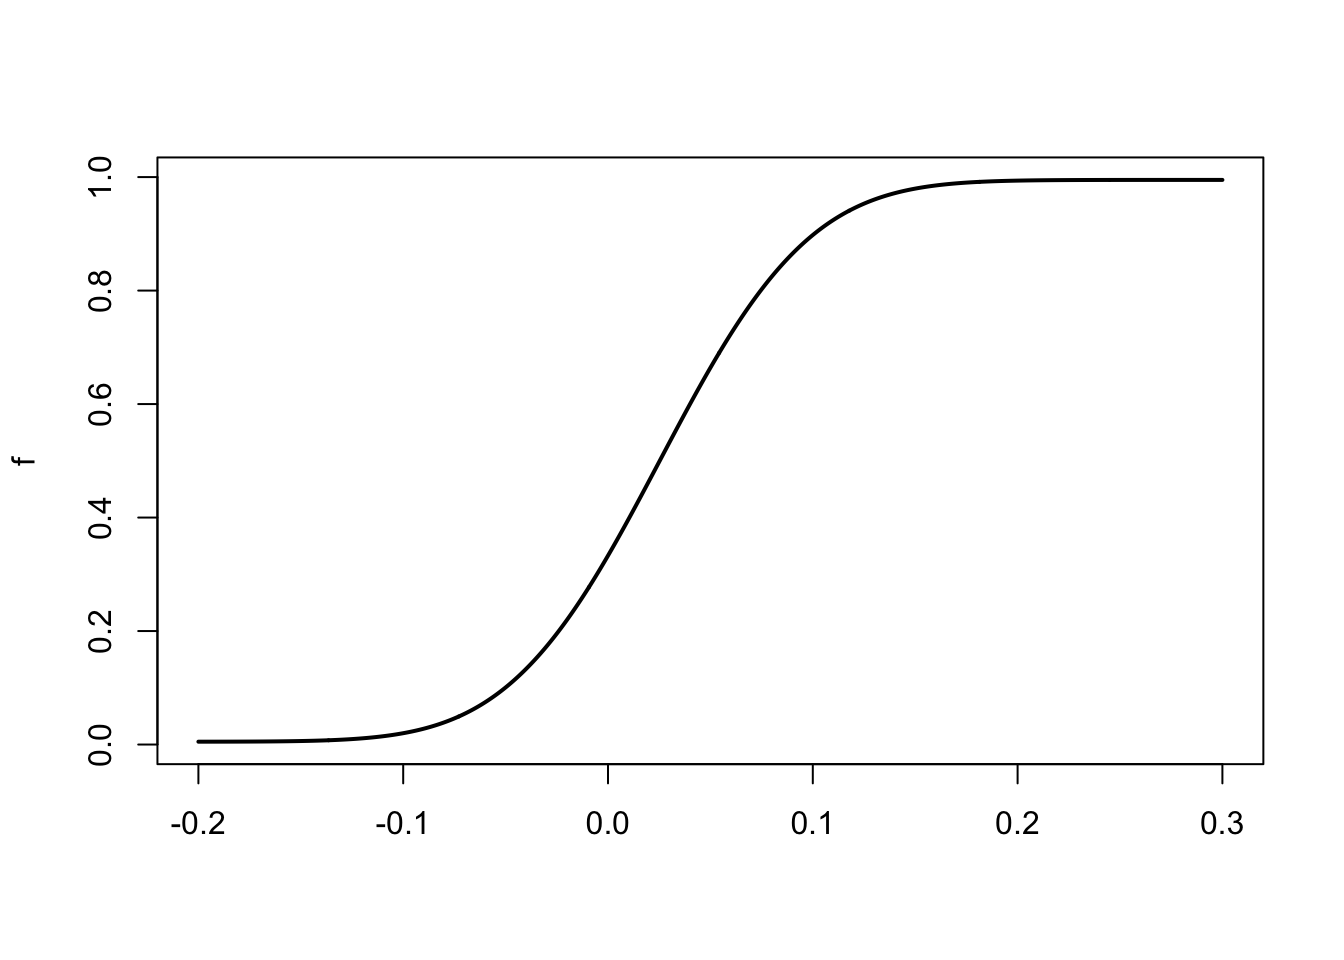
\includegraphics{TSM_files/figure-latex/truncatedRR-1} \caption{Conditional cumulated distribution function (c.d.f.) of $\frac{1}{H}(r_{t+1}+\dots+r_{t+H})$.}\label{fig:truncatedRR}
\end{figure}

\end{example}

\hypertarget{appendices}{%
\section{Appendices}\label{appendices}}

\begin{lemma}
\protect\hypertarget{lem:integralQuadratic}{}\label{lem:integralQuadratic}If \(\mu \in \mathbb{R}^L\) and \(Q\) is a \((L \times L)\) matrix symmetric positive definite, then:
\[
\int_{\mathbb{R}^{L}} \exp(-u'Q u + \mu'u)du =
\frac{\pi^{L/2}}{(det   Q)^{1/2}} exp \left(
\begin{array}{l}  \frac{1}{4} \mu'Q^{-1}\mu \end{array} \right).
\]
\end{lemma}

\begin{proof}
The integral is:
\begin{eqnarray*}
&& \int_{\mathbb{R}^{L}} exp \left[ \begin{array}{l} - (u -
\frac{1}{2}  Q^{-1} \mu)'  Q (u -
\frac{1}{2} Q^{-1} \mu)'
\end{array}
\right] exp\left(
\begin{array}{l}  \frac{1}{4} \mu'Q^{-1}\mu \end{array}
\right)du \\
&=&  \frac{\pi^{L/2}}{(det Q)^{1/2}} exp\left(
\begin{array}{l}  \frac{1}{4} \mu'Q^{-1}\mu \end{array}
\right)
\end{eqnarray*}
{[}using the formula for the unit mass of \(\mathcal{N}( 0.5Q^{-1}\mu,(2Q)^{-1})\){]}.
\end{proof}

\begin{lemma}
\protect\hypertarget{lem:Quadr}{}\label{lem:Quadr}If \(\varepsilon_{t+1} \sim \mathcal{N}(0,Id)\), we have
\[
\mathbb{E}_t \left(\exp[\lambda'\varepsilon_{t+1}+\varepsilon'_{t+1} V \varepsilon_{t+1}]\right) =  \frac{1}{[\det(I-2V)]^{1/2}} \exp\left[
\frac{1}{2} \lambda'(I-2V)^{-1}\lambda
\right].
\]
\end{lemma}

\begin{proof}
We have
\[
\mathbb{E}_t   \exp(\lambda'\varepsilon_{t+1}+\varepsilon'_{t+1}V\varepsilon_{t+1})
=  \frac{1}{(2\pi)^{n/2}}  \int_{\mathbb{R}^{n}} \exp\left[
\begin{array}{l}
-u'\left(
\begin{array}{l}
\frac{1}{2} I-V
\end{array}
\right)u+\lambda'u
\end{array}
\right]du
\]
From Lemma \ref{lem:integralQuadratic}, if \(u\in\mathbb{R}^n\), then
\[
\int_{\mathbb{R}^{n}} \exp(-u' Q u+\mu'u) du =
\frac{\pi^{n/2}}{(\det Q)^{1/2}} \exp\left(
\begin{array}{l}
\frac{1}{4} \mu'Q^{-1}\mu
\end{array}
\right).
\]
Therefore:
\[
\begin{array}{l}
\mathbb{E}_t   \exp(\lambda'\varepsilon_{t+1}+\varepsilon'_{t+1}V\varepsilon_{t+1}) \\
=  \frac{1}{2^{n/2}
\left[
\begin{array}{l}
\det \left(
\begin{array}{l}
\frac{1}{2} I-V
\end{array}
\right)
\end{array}
\right]^{1/2}
}
\exp\left[
\begin{array}{l}
\frac{1}{4}  \lambda'\left(
\begin{array}{l}
\frac{1}{2} I-V
\end{array}
\right)^{-1}\lambda
\end{array}
\right].
\end{array}
\]
\end{proof}

\begin{proposition}[Quadratic Gaussian process]
\protect\hypertarget{prp:QGVAR1}{}\label{prp:QGVAR1}Consider vector \(w_t = (x'_t,vec(x_t x_t')')'\), where \(x_t\) is a \(n\)-dimensional vector following a Gaussian VAR(1), i.e.
\[
x_{t+1}|\underline{w_t} \sim \mathcal{N}(\mu+\Phi x_t, \Sigma).
\]
If \(u = (v,V)\) where \(v \in \mathbb{R}^n\) and \(V\) a square symmetric matrix of size \(n\), we have:
\begin{eqnarray*}
\varphi_t(u) &=& \mathbb{E}_t\big\{\exp\big[(v',vec(V)')\times w_{t+1}\big]\big\} \\
& =& \exp \left\{a_1(v,V)'x_t +vec(a_2(v,V))' vec(x_t'x_t) + b(v,V) \right\},
\end{eqnarray*}
where:
\begin{eqnarray*}
a_2(u) & = & \Phi'V (I_n - 2\Sigma V)^{-1} \Phi \nonumber \\
a_1(u) & = & \Phi'\left[(I_n-2V\Sigma)^{-1}(v+2V\mu)\right] \nonumber \\
b(u) & = & u'(I_n - 2 \Sigma V)^{-1}\left(\mu + \frac{1}{2} \Sigma v\right) +\\
&& \mu'V(I_n - 2 \Sigma V)^{-1}\mu - \frac{1}{2}\log\big|I_n - 2\Sigma V\big|.\label{eq:laplaceZ}
\end{eqnarray*}
\end{proposition}

\begin{proof}
We have:
\begin{eqnarray*}
&&\mathbb{E}_t(\exp(v' x_{t+1} + vec(V)'vec(x_{t+1} x_{t+1}'))) \\
&=& \mathbb{E}_t[\exp(v' (\mu + \Phi x_t + \Sigma^{1/2}\varepsilon_{t+1}) + \\
&& vec(V)'vec((\mu + \Phi x_t + \Sigma^{1/2}\varepsilon_{t+1}) (\mu + \Phi x_t + \Sigma^{1/2}\varepsilon_{t+1})'))] \\
&=& \exp[v' (\mu + \Phi x_t) + vec(V)'vec\{(\mu + \Phi x_t)(\mu + \Phi x_t)'\}] \times \\
&& \mathbb{E}_t[\exp(v'\Sigma^{1/2}\varepsilon_{t+1} +2\underbrace{ vec(V)' vec\{(\mu + \Phi x_t)(\varepsilon_{t+1}'{\Sigma^{1/2}}')\}}_{=(\mu + \Phi x_t)'V\Sigma^{1/2}\varepsilon_{t+1}} +\\
&& \underbrace{vec(V)'vec\{(\Sigma^{1/2}\varepsilon_{t+1})(\Sigma^{1/2}\varepsilon_{t+1})'}_{=\varepsilon_{t+1}'{\Sigma^{1/2}}'V\Sigma^{1/2}\varepsilon_{t+1}}\}]
\end{eqnarray*}
Lemma \ref{lem:Quadr} can be used to compute the previous conditional expectation, with \(\lambda = {\Sigma^{1/2}}'(v + 2 V'(\mu + \Phi x_t))\). Some algebra then leads to the result.
\end{proof}

\begin{proposition}[]
\protect\hypertarget{prp:LTARG}{}\label{prp:LTARG}Consider the following auto-regressive gamma process:
\[
\frac{w_{t+1}}{\mu} \sim \gamma(\nu+z_t) \quad \mbox{where} \quad z_t \sim \mathcal{P} \left( \frac{\rho w_t}{\mu} \right),
\]
with \(\nu\), \(\mu\), \(\rho > 0\). (Alternatively \(z_t \sim {\mathcal{P}}(\beta w_t)\), with \(\rho = \beta \mu\).)

We have:
\(\varphi_t(u) = exp \left[ \begin{array}{l} \dfrac{\rho u}{1-u \mu} w_t - \nu \log(1-u \mu)\end{array} \right], \mbox{ for } u < \dfrac{1}{\mu}\).
\end{proposition}

\begin{proof}
Given \(\underline{w_t}\), we have \(z_t \sim {\mathcal P}\left( \begin{array}{l} \frac{\rho w_t} {\mu} \end{array}\right)\). We have:
\begin{eqnarray*}
\mathbb{E}[\exp(u w_{t+1})|\underline{w_t}] &=& \mathbb{E}\left\{\mathbb{E}\left[\exp \left(u \mu  \frac{w_{t+1}}{\mu}\right)|\underline{w_t}, \underline{z}_t\right]\underline{w_t}\right\}\\
&=& \mathbb{E}[(1-u\mu)^{-(\nu+z_t)}|\underline{w_t}] \\
&=& (1-u\mu)^{-\nu}\mathbb{E}\{\exp[-z_t   \log(1-u\mu)]|\underline{w_t}\} \\
&=& (1-u\mu)^{-\nu} \exp \left\{\frac{\rho w_t}{\mu}[\exp(-\log(1-u\mu)] -  \frac{\rho w_t}{\mu}\right\}\\
&=& \exp\left[ \begin{array}{l}  \frac{\rho u w_t}{1-u\mu} - \nu   \log(1-u\mu)  \end{array}\right],
\end{eqnarray*}
using the fact that the L.T. of \(\gamma(\nu)\) is \((1-u)^{-\nu}\)
and that the L.T. of \({\mathcal P}(\lambda)\) is \(\exp[\lambda(\exp(u)-1)]\).
\end{proof}

\begin{proposition}[Dynamics of a WAR process]
\protect\hypertarget{prp:WARAR}{}\label{prp:WARAR}If \(K\) is an integer, \(W_{t+1}\) can be obtained from:
\begin{eqnarray*}
\left\{
\begin{array}{ccl}
W_{t+1} & =&  \sum^K_{k=1} x_{k,t+1} x'_{k,t+1}\\
&&\\
x_{k,t+1} & =& M x_{k,t} + \varepsilon_{k,t+1},\quad k \in \{1,\dots,K\},
\end{array}
\right.
\end{eqnarray*}
where \(\varepsilon_{k,t+1} \sim i.i.d. \mathcal{N}(0, \Omega)\) (independent across \(k\)'s).
In particular, we have:
\[
\mathbb{E}(W_{t+1}|\underline{W_t}) = MW_tM'+K \Omega,
\]
i.e.~\(W_t\) follows a matrix weak AR(1) process.
\end{proposition}

\begin{proof}
For \(K=1\), \(W_{t+1}=x_{t+1} x'_{t+1}\), \(x_{t+1} = M x_t + \Omega^{1/2} u_{t+1}\) and \(u_{t+1} \sim i.i.d. \mathcal{N}(0,Id_L)\). We have:
\[
\mathbb{E}[\exp(Tr \Gamma W_{t+1})|\underline{w_t}] = \mathbb{E}\{\mathbb{E}[\exp(Tr \Gamma x_{t+1} x'_{t+1})|\underline{x}_t]|\underline{w_t}\}
\]
and:
\begin{eqnarray*}
&& \mathbb{E}[\exp(Tr \Gamma x_{t+1}x'_{t+1})|\underline{x}_t] = \mathbb{E}[\exp(x'_{t+1}\Gamma x_{t+1}|\underline{x}_t] \\
&=& \mathbb{E}[\exp(M x_t + \Omega^{1/2} u_{t+1})'\Gamma(M x_t + \Omega^{1/2} u_{t+1})/x_t] \\
&=& \exp(x'_tM'\Gamma M x_t)\mathbb{E}[\exp(2 x'_t M'\Gamma \Omega^{1/2}
u_{t+1}+u'_{t+1}\Omega^{1/2} \Gamma \Omega^{1/2} u_{t+1})/x_t] \\
&=&  \frac{exp(x'_tM'\Gamma M x_t)}{(2\pi)^{L/2}} \times \\
&& \int_{\mathbb{R}^L} \exp\left[2x'_tM'\Gamma
\Omega^{1/2}u_{t+1}-u'_{t+1}\left(
\frac{1}{2} Id_L-\Omega^{1/2} \Gamma \Omega^{1/2}\right)u_{t+1}\right]  du_{t+1}.
\end{eqnarray*}
Using Lemma \ref{lem:integralQuadratic} with \(\mu' = 2 x'_t M'\Gamma \Omega^{1/2}, Q = \frac{1}{2} Id_L-\Omega^{1/2}\Gamma\Omega^{1/2}\) \textbackslash{}
and after some algebra, the RHS becomes:
\[
\frac{exp[x'_tM'\Gamma(Id_L-2\Omega\Gamma)^{-1}M
x_t]}{det[Id_L-2\Omega^{1/2}\Gamma\Omega^{1/2}]} =  \frac{exp Tr[M'\Gamma(Id_L-2\Omega^{-1}]M
W_t]}{det[Id_L-2\Omega \Gamma]^{1/2}},
\]
which depends on \(x_t\) through \(W_t\), and gives the result for
\(K=1\); the result for any \(K\) integer follows.
\end{proof}

\begin{lemma}
\protect\hypertarget{lem:MHLT}{}\label{lem:MHLT}We have:
\[
\varphi_{t,h}(\gamma_1,\dots,\gamma_h) = \exp(A'_{t,h} w_t + B_{t,h}),
\]
where \(A_{t,h} = A^h_{t,h}\) and \(B_{t,h} = B^h_{t,h}\), the \(A^h_{t,i}, B^h_{t,i}\) \(i = 1,\dots,h\), being given recursively by:
\[
(i) \left\{
\begin{array}{ccl}
A^h_{t,i} &=& a_{t+h+1-i}(\gamma_{h+1-i} + A^h_{t,i-1}), \\
B^h_{t,i} &=& b_{t+h+1-i}(\gamma_{h+1-i} + A^h_{t,i-1}) + B^h_{t,i-1}, \\
A^h_{t,0} &=& 0, B^h_{t,0} = 0.
\end{array}
\right.
\]
\end{lemma}

\begin{proof}
For any \(j=1,\dots,h\) we have:
\[
\varphi_{t,h}(\gamma_1,\dots,\gamma_h) = \mathbb{E}_t[\exp(\gamma'_1 w_{t+1}+\dots\gamma'_j w_{t+j}+A^{h'}_{t,h-j}w_{t+j}+B^h_{t,h-j})]
\]
where:
\[
(ii) \left\{
\begin{array}{l}
A^h_{t,h-j+1} = a_{t+j}(\gamma_{j} + A^h_{t,h-j}), \\
B^h_{t,h-j+1} = b_{t+j}(\gamma_{j} + A^h_{t,h-j}) + B^h_{t,h-j}, \\
A^h_{t,0} = 0, B^h_{t,0} = 0.
\end{array}
\right.
\]
Since this is true for \(j=h\), and if this is true for \(j\), we get:
\[
\begin{array}{ll}
\varphi_{t,h}(\gamma_1,\dots,\gamma_h) & = \mathbb{E}_t [\exp(\gamma'_1 w_{t+1}+\dots+\gamma'_{j-1}w_{t+j-1}+a'_{t+j}(\gamma_j+A^h_{t,h-j})w_{t+j-1} \\
& + b_{t+j}(\gamma_j+A^h_{t,h-j})+B^h_{t,h-j}],
\end{array}
\]
and, therefore, this is true for \(j-1\), with \(A^h_{t,h-j+1}\) and \(B^h_{t,h-j+1}\) given by formulas (ii) above.

For \(j=1\) we get:
\begin{eqnarray*}
\varphi_{t,h}(\gamma_1,\dots,\gamma_h) &=& \mathbb{E}_t \exp(\gamma'_1 w_{t+1}+A^{h'}_{t,h-1}w_{t+1}+B^h_{t,h-1}) \\
&=& \exp(A'_{t,h} w_t+B_{t,h}),
\end{eqnarray*}

Finally note that if we put \(h-j+1 = i\), formulas (ii) become (i).
\end{proof}

\begin{proposition}[Reverse-order multi-horizon Laplace transform]
\protect\hypertarget{prp:reverseMLT}{}\label{prp:reverseMLT}If the functions \(a_{t}\) and \(b_{t}\) do not depend on \(t\), and if different sequences \((\gamma^h_1,\dots,\gamma^h_h), h=1,\dots,H\) (say) satisfy \(\gamma^h_{h+1-i} = u_i\), for
\(i=1,\dots,h\), and for any \(h \leq H\), that is if we want to compute (``reverse order'' case):
\[
\varphi_{t,h}(u_h,\dots,u_1)=\mathbb{E}_t[\exp(u'_{\color{red}{h}} w_{\color{red}{t+1}}+\dots+u'_{\color{red}{1}} w_{\color{red}{t+h}})],
\quad h=1,\dots,H,
\]
then we can compute the \(\varphi_{t,h}(u_h,\dots,u_1)\) for any \(t\) and any \(h \leq H\), with only one recursion, i.e.~\(\varphi_{t,h}(u_h,\dots,u_1)=\exp(A'_hw_t+B_h)\) with:
\begin{equation}
\left\{
\begin{array}{ccl}
A_{h} &=& a(u_{h} + A_{h-1}), \\
B_{h} &=& b(u_{h} + A_{h-1}) + B_{h-1}, \\
A_{0} &=& 0,\quad  B_{0} = 0.
\end{array}
\right.\label{eq:auxLemmareverseMLT}
\end{equation}
\end{proposition}

\begin{proof}
According to Lemma \ref{lem:MHLT}, we have, in this case:
\[
\left\{
\begin{array}{ccl}
A^h_{i} &=& a(u_{i} + A^h_{i-1}), \\
B^h_{i} &=& b(u_{i} + A^h_{i-1}) + B^h_{i-1}, \\
A^h_{0} &=& 0, \quad B^h_{0} = 0.
\end{array}
\right.
\]
The previous sequences do not dependent on \(h\) and are given by Eq. \eqref{eq:auxLemmareverseMLT}.
\end{proof}

\begin{proposition}[Conditional means and variances of an affine process]
\protect\hypertarget{prp:condvarAffine}{}\label{prp:condvarAffine}Consider an affine process \(w_t\). Using the notation of Proposition \ref{prp:affineVAR}, we have:
\begin{eqnarray}
\mathbb{E}_t(w_{t+h}) &=& (I - \Phi)^{-1}(I - \Phi^h)\mu + \Phi^h w_t \label{eq:condmeanAppendix}\\
\mathbb{V}ar_t(w_{t+h}) &=& \Sigma(\mathbb{E}_t(w_{t+h-1}))+\Phi \Sigma(\mathbb{E}_t(w_{t+h-2}))\Phi' + \nonumber \\
&& \dots + \Phi^{h-1} \Sigma(w_{t}){\Phi^{h-1}}'. \label{eq:condvarAppendix}
\end{eqnarray}
Eq. \eqref{eq:condvarAppendix} notably shows that \(\mathbb{V}ar_t(w_{t+h})\) is an affine function of \(w_t\). Indeed \(\Sigma(.)\) is an affine function, and the conditional expectations \(\mathbb{E}_t(w_{t+h})\) are affine in \(w_t\), as shown by Eq. \eqref{eq:condmeanAppendix}.

The unconditional mean and variance of \(w_t\) are given by:
\begin{equation}
\left\{
\begin{array}{ccl}
\mathbb{E}(w_t) &=& (I - \Phi)^{-1}\mu\\
vec[\mathbb{V}ar(w_t)] &=& (I_{n^2} - \Phi \otimes \Phi)^{-1} vec\left(\Sigma[(I - \Phi)^{-1}\mu]\right).
\end{array}
\right.\label{eq:uncondmeanvarAppendix}
\end{equation}
\end{proposition}

\begin{proof}
Eq. \eqref{eq:condmeanAppendix} is easily deduced from Eq. \eqref{eq:VARw}, using that \(\mathbb{E}_t(\varepsilon_{t+k})=0\) for \(k>0\).

As regards Eq. \eqref{eq:condvarAppendix}:
\begin{eqnarray*}
\mathbb{V}ar_t(w_{t+h}) &=& \mathbb{V}ar_t\left(\Sigma(w_{t+h-1})^{\frac{1}{2}}\varepsilon_{t+h}+\dots + \Phi^{h-1} \Sigma(w_{t})^{\frac{1}{2}}\varepsilon_{t+1} \right).
\end{eqnarray*}
The conditional expectation at \(t\) of all the terms of the sum is equal to zero since, for \(i \ge 1\):
\[
\mathbb{E}_t\left[\Sigma(w_{t+i-1})^{\frac{1}{2}}\varepsilon_{t+i}\right] = \mathbb{E}_t[\underbrace{\mathbb{E}_{t+i-1}\{\Sigma(w_{t+i-1})^{\frac{1}{2}}\varepsilon_{t+i}\}}_{=\Sigma(w_{t+i-1})^{\frac{1}{2}}\mathbb{E}_{t+i-1}\{\varepsilon_{t+i}\}=0}\}],
\]
and \(\forall i <j\),
\[
\mathbb{C}ov_t\left[\Sigma(w_{t+i-1})^{\frac{1}{2}}\varepsilon_{t+i},\Sigma(w_{t+j-1})^{\frac{1}{2}}\varepsilon_{t+j}\right] = \mathbb{E}_t\left[\Sigma(w_{t+i-1})^{\frac{1}{2}}\varepsilon_{t+i}\varepsilon_{t+j}'\Sigma'(w_{t+j-1})^{\frac{1}{2}}\right],
\]
which can be seen to be equal to zero by conditioning on the information available on date \(t+j-1\).

Using the same conditioning, we obtain that:
\begin{eqnarray*}
\mathbb{V}ar_t\left[\Phi^{h-j}\Sigma(w_{t+j-1})^{\frac{1}{2}}\varepsilon_{t+j}\right] &=& \mathbb{E}_t\left[\Phi^{h-j}\Sigma(w_{t+j-1})^{\frac{1}{2}}\varepsilon_{t+j}\varepsilon_{t+j}'\Sigma'(w_{t+j-1})^{\frac{1}{2}}{\Phi^{h-j}}'\right] \\
&=&  \mathbb{E}_t\left[\Phi^{h-j}\Sigma(w_{t+j-1})^{\frac{1}{2}} \mathbb{E}_{t+j-1}(\varepsilon_{t+j}\varepsilon_{t+j}')\Sigma'(w_{t+j-1})^{\frac{1}{2}}{\Phi^{h-j}}'\right] \\
&=&  \Phi^{h-j}\mathbb{E}_t[\Sigma(w_{t+j-1})]{\Phi^{h-j}}' \\
&=&  \Phi^{h-j}\Sigma(\mathbb{E}_t[w_{t+j-1}]){\Phi^{h-j}}',
\end{eqnarray*}
where the last equality results from the fact that he fact that \(\Sigma(.)\) is affine (see Eq. \eqref{eq:SigmaWt}).
\end{proof}

\begin{proposition}[Affine property of the GARCH-type process]
\protect\hypertarget{prp:GARCH}{}\label{prp:GARCH}The process \(w_t = (w_{1,t}, w_{2,t})\) defined by:
\[
\left\{
\begin{array}{ccl}
w_{1, t+1} &=& \mu + \varphi w_{1,t} + \sigma_{t+1} \varepsilon_{t+1}    \mid \varphi \mid < 1 \\
\sigma^2_{t+1} &=& \omega + \alpha \varepsilon^2_t + \beta \sigma^2_t      0 < \beta < 1, \alpha > 0, \omega > 0    \\
w_{2,t} &=& \sigma^2_{t+1}, \quad \varepsilon_t \sim   i.i.d.   \mathcal{N}(0,1)
\end{array}
\right.
\]
is affine.
\end{proposition}

\begin{proof}
Note that \(w_{2,t}\) is function of \(\underline{w_{1,t}}\)
\begin{eqnarray*}
&& \mathbb{E}[\exp(u_1 w_{1, t+1} + u_2 w_{2, t+1})|\underline{w_{1,t}}] \\
&= & \exp(u_1 \mu + u_1 \varphi w_{1,t} + u_2 \omega + u_2 \beta w_{2,t})  \mathbb{E}[\exp(u_1 \sigma_{t+1} \varepsilon_{t+1} + u_2 \alpha \varepsilon^2_{t+1})|\underline{w_{1,t}}]
\end{eqnarray*}
and, using Lemma \ref{lem:Quadr}:
\begin{eqnarray*}
&&\mathbb{E}[\exp(u_1 w_{1, t+1} + u_2 w_{2, t+1})|\underline{w_{1,t}}] \\
&= & \exp(u_1 \mu + u_1 \varphi w_{1,t} + u_2 \omega + u_2 \beta w_{2t})  \exp \left[ -   \frac{1}{2}   \log(1-2 u_2 \alpha) +
\frac{u^2_1 w_{2,t}}{2(1-2 u_2 \alpha)} \right]\\
&= & \exp \left[ u_1 \mu + u_2 \omega -  \frac{1}{2}   \log(1-2u_2\alpha)+  u_1 \varphi w_{1,t} + \left(u_2 \beta +  \frac{u^2_1}{2(1-2u_2\alpha)}\right)
w_{2,t}\right],
\end{eqnarray*}
which is exponential affine in \((w_{1,t}, w_{2,t})\).
\end{proof}

\begin{proposition}[Computation of truncated conditional moments]
\protect\hypertarget{prp:Fourier}{}\label{prp:Fourier}If \(\varphi(z)=\mathbb{E}[exp(z'w)]\), we have:
\begin{equation}
\mathbb{E}[\exp(u'w)\textbf{1}_{(v'w<\gamma})] = \frac{\varphi(u)}{2} -  \frac{1}{\pi} \int^\infty_o
\frac{{\mathcal I}m[\varphi(u+ivx)\exp(-i\gamma x)]}{x}dx.\label{eq:Truncated}
\end{equation}
\end{proposition}

\begin{proof}
We want to compute \(\tilde{\varphi}_t(u;v,\gamma) = \mathbb{E}_t[\exp(u'w)\textbf{1}_{(v'w<\gamma})]\). Let us first note that, for given \(u\) and \(v\), \(\tilde{\varphi}_t(u;v,\gamma)\) is a positive increasing bounded function of \(\gamma\) and therefore can be seen as the c.d.f. of a positive finite measure on \(\mathbb{R}\), the Fourier transform of which is:
\[
\int_{\mathbb{R}} \exp(i\gamma x)d\tilde{\varphi}(u;v,\gamma) = \mathbb{E} \int_{\mathbb{R}} \exp(i\gamma x)d\tilde{\varphi}_w(u;v,\gamma),
\]
where, for given \(w, \tilde{\varphi}_w(u;v,\gamma)\) is the c.d.f. of the mass point \(\exp(u'w)\) at \(v'w\). We then get:
\begin{eqnarray*}
\int_{\mathbb{R}} \exp(i\gamma x) d\tilde{\varphi}(u;v,\gamma) &=& \mathbb{E}[\exp(ixv'w)exp(u'w)] \\
& =& \mathbb{E}[\exp(u+ivx)'w] \\
& =& \varphi(u+ivx).
\end{eqnarray*}
Let us now compute \(A(x_0,\lambda)\) for any real number \(\lambda\), with:
\begin{eqnarray*}
&&A(x_0,\lambda) \\
&=&  \frac{1}{2\pi} \int^{x_0}_{-x_0}
\frac{\exp(i\lambda x)\varphi(u-ivx)-\exp(-i\lambda)\varphi(u+ivx)}{ix}dx \\
&=&  \frac{1}{2\pi} \int^{x_0}_{-x_0}\left[ \begin{array}{l}  \int_{\mathbb{R}}
\frac{\exp[-ix(\gamma-\lambda)]-\exp[ix(\gamma-\lambda)]}{ix}d\tilde{\varphi}(u;v,\gamma)
\end{array} \right]dx \\
&=&  \frac{1}{2\pi}  \int_{\mathbb{R}}
\left[ \begin{array}{l}   \int^{x_0}_{-x_0}   \frac{\exp[-ix(\gamma-\lambda)]
-\exp[ix(\gamma-\lambda)]}{ix}dx \end{array} \right]d\tilde{\varphi}(u;v,\gamma).
\end{eqnarray*}
Now :
\begin{eqnarray*}
\frac{1}{2\pi} \int^{x_o}_{-x_o}
\frac{\exp[-ix(\gamma-\lambda)]
-\exp[ix(\gamma-\lambda)]}{ix}dx \\ =  \frac{-sign(\gamma-\lambda)}{\pi}
\int^{x_o}_{-x_o} \frac{sin(x\mid\gamma-\lambda\mid)}{x}dx
\end{eqnarray*}
which tends to \(-sign(\gamma-\lambda)\) when \(x_0\rightarrow\infty\) (where \(sign(\omega)=1\) if \(\omega>0\), \(sign(\omega)=0\) if \(\omega=0\), \(sign(\omega)=-1\) if \(\omega<0\)).
Therefore:
\[
A(\infty,\lambda) = -  \int_{\mathbb{R}} sign(\gamma-\lambda)d\tilde{\varphi}(u;v,\gamma) = -\mathbb{E}  \int_{\mathbb{R}} sign(\gamma-\lambda)d\tilde{\varphi}_w(u;\theta,\gamma),
\]
where \(\tilde{\varphi}_w(u;v,\gamma)\) is the c.d.f. of the mass point \(\exp(u'w)\) at \(v'w\) and
\[
\int_{\mathbb{R}} \mbox{sign}(\gamma-\lambda)d\tilde{\varphi}_w(u;v,\gamma)=
\left\{
\begin{array}{ccc}
\exp(u'w) & \mbox{if} & \lambda < v'w \\
0 & \mbox{if}& \lambda = v'w \\
-\exp(u'w) & \mbox{if} & \lambda > v'w.
\end{array}
\right.
\]
Therefore, we have:
\begin{eqnarray*}
A(\infty,\lambda) & =& - \mathbb{E}[\exp(u'w)(1-\textbf{1}_{(v'w<\lambda)})-\exp(u'w)\textbf{1}_{(v'w<\lambda)}] \\
& =& - \varphi(u) + 2\tilde{\varphi}(u;v,\lambda)
\end{eqnarray*}
and, further,:
\[
\tilde{\varphi}(u;,v,\gamma) =  \frac{\varphi(u)}{2} +  \frac{1}{2} A(\infty,\gamma),
\]
where
\begin{eqnarray*}
\frac{1}{2} A(\infty,\gamma) & =&  \frac{1}{4\pi} \int^{\infty}_{-\infty}  \frac{\exp(i\gamma x)\varphi(u-ivx)-\exp(-i\gamma x)\varphi(u+ivx)}{ix} dx \\
& =&  \frac{1}{2\pi} \int^{\infty}_{o}  \frac{\exp(i\gamma x)\varphi(u-ivx)-\exp(-i\gamma x)\varphi(u+ivx)}{ix} dx \\
& =& -  \frac{1}{\pi} \int^{\infty}_{o}  \frac{{\mathcal I}m[\exp(-i\gamma x)\varphi(u+ivx)]}{x}dx,
\end{eqnarray*}
which leads to Eq. \eqref{eq:Truncated}.
\end{proof}

\hypertarget{Structural}{%
\chapter{A detour through structural approaches}\label{Structural}}

In this chapter, we introduce structural approaches that have been used to investigate asset pricing. \emph{Structural models} aim to link the stochastic discount factor (SDF) to investor risk preferences. Investors make portfolio decisions to obtain a desired time and risk profile of consumption. Loosely speaking, in structural asset-pricing models, the SDF \(\mathcal{M}_{t,t+1}\) captures the aspects of utility that matter for valuing the assets.

\hypertarget{PricingEquilibrium}{%
\section{Consumption-based Capital Asset Pricing Model (CCAPM) and stochastic discount factor (SDF)}\label{PricingEquilibrium}}

A seminal example of structural asset-pricing model is that of the consumption capital asset pricing model, or CCAPM (see, e.g., \citet{Merton_1973} and \citet{BREEDEN1979265}). The CCAPM extends the CAPM framework by providing a consumption-based theory of the determinants of the valuation of the market portfolio.

\hypertarget{the-sdf-when-agents-feature-expected-utility-time-separable-preferences}{%
\subsection{The SDF when agents feature expected-utility time-separable preferences}\label{the-sdf-when-agents-feature-expected-utility-time-separable-preferences}}

Consider an economy featuring a single good, whose date-\(t\) price is \(q_t\). There is a representative agent with an external income \(Y_t\) at \(t\), and a portfolio of assets, with an allocation vector \(\alpha_{t-1}\) (decided at \(t-1\)). The vector of date-\(t\) prices is \(p_t\). At any date \(t+j\), \(j=0,1,\dots\), the agent will face the budget constraint:
\begin{equation}
q_{t+j}C_{t+j}+\alpha'_{t+j}p_{t+j} = Y_{t+j} +
\alpha'_{t+j-1}p_{t+j},\label{eq:BConstr}
\end{equation}
where \(C_{t+j}\)is her consumption on date \(t+j\).

In the standard CCAPM, agents maximize their intertemporal utility that is of the Expected-Utility Time-Separable type (see Def. \ref{def:EUTSpref}).

\begin{definition}[Expected-utility time-separable preferences]
\protect\hypertarget{def:EUTSpref}{}\label{def:EUTSpref}In the context of \emph{expected-utility time-separable preferences}, the intertemporal utility \(U_t\) is defined as:
\[
U_t = \mathbb{E}_t\left(\sum_{i=0}^{\infty} \delta^{i}u(C_{t+i})\right),
\]
or, equivalently, as:
\[
U_t = u(C_t) + \delta \mathbb{E}_t\left(U_{t+1}\right).
\]
\(U\) is the utility function and \(\delta\) is the pure preference for present, or subjective discount factor.
\end{definition}

\begin{quote}
Importantly, the pure preference for present (\(\delta\)) is different from the stochastic discount factor (SDF).
\end{quote}

The representative agent maximizes her expected utility time-separable preferences (see Definition \ref{def:EUTSpref}) subject to the budget constraints at \(t+j\), \(j \ge 0\), see Eq. \eqref{eq:BConstr}.

Replacing \(C_{t+j}\) with \([Y_{t+j}-(\alpha'_{t+j}-\alpha'_{t+j-1})p_{t+j}]/q_{t+j}\), the objective function becomes:
\[
\mathbb{E}_t  \sum^\infty_{j=0} \delta^j U
[Y_{t+j}/q_{t+j}-(\alpha'_{t+j}-\alpha'_{t+j-1})p_{t+j}/q_{t+j}].
\]
The vector of allocation \(\alpha_t\) appears in the first two terms only:
\[
U[Y_t/q_t-(\alpha'_t-\alpha'_{t-1})p_t/q_t] + \delta \mathbb{E}_t
U[Y_{t+1}/q_{t+1}-(\alpha'_{t+1}-\alpha'_t)p_{t+1}/q_{t+1}].
\]
As a result, the first order condition associated with vector \(\alpha_t\) reads
\[
\frac{p_t}{q_t}  \frac{d U(C_t)}{dC} = \delta \mathbb{E}_t \left[
\frac{p_{t+1}}{q_{t+1}}  \frac{dU(C_{t+1})}{dC}
\right],
\]
or
\begin{equation}
p_t = \mathbb{E}_t(p_{t+1} \mathcal{M}_{t,t+1}),\label{eq:SDF100}
\end{equation}
where \(\mathcal{M}_{t,t+1}\) is a strictly positive scalar called \emph{stochastic discount factor (SDF)} between dates \(t\) and \(t+1\). We have:
\begin{equation}
\mathcal{M}_{t,t+1} \equiv \delta  \frac{q_t}{q_{t+1}}
\frac{  \frac{dU(C_{t+1})}{dC}} {
\frac{dU(C_t)}{dC}}.\label{eq:SDFCCAPM}
\end{equation}

According to Eq. \eqref{eq:SDF100}, for any asset \(j\):
\begin{equation}
p_{j,t} = \mathbb{E}_t(\mathcal{M}_{t,t+1} p_{j,t+1}).\label{eq:Mbasicpricing}
\end{equation}
Using that \(p_{j,t+1} = \mathbb{E}_t(\mathcal{M}_{t+1,t+2} p_{j,t+2})\), we get:
\begin{eqnarray*}
p_{j,t} &=& \mathbb{E}_t[\mathbb{E}_{t+1}(p_{j,t+2}\mathcal{M}_{t+1,t+2})\mathcal{M}_{t,t+1}] \\
&=& \mathbb{E}_t(\mathcal{M}_{t,t+1} \mathcal{M}_{t+1,t+2}p_{j,t+2}).
\end{eqnarray*}
This can be generalized as follows, for \(h \ge 1\):
\[
p_{j,t} = \mathbb{E}_t[\mathcal{M}_{t,t+1} \dots \mathcal{M}_{t+h-1,t+h}p_{j,t+h}] = \mathbb{E}_t[\mathcal{M}_{t,t+h}p_{j,t+h}].
\]

Since \(u'\) is a decreasing function, \eqref{eq:SDFCCAPM} implies that, the lower \(C_{t+1}\), the higher the SDF. Moreover, \eqref{eq:Mbasicpricing} shows that those assets whose payoffs are high during recessions (low \(C_{t+1}\)) are more valuable. As \citet{Cochrane_2005} puts it, the SDF can be seen as a measure of hunger: ``Good'' assets pay off well in bad times, when investors are hungry. Investors all want them, which drive up their price, and thereby lower their average returns.

Eq. \eqref{eq:Mbasicpricing} rewrites:
\begin{equation}
p_{j,t} = \mathbb{C}ov_t(\mathcal{M}_{t,t+1},p_{j,t+1}) +\mathbb{E}_t(\mathcal{M}_{t,t+1})\mathbb{E}_t(p_{j,t+1}).\label{eq:covpM1}
\end{equation}

Consider the one-period risk-free bond, whose payoff, on date \(t+1\), is 1 unit. The price of this asset, on the current date (\(t\)) is \(\frac{1}{1+R_{f,t}}\)---by definition of the short-term risk free rate \(R_{f,t}\). Eq. \eqref{eq:Mbasicpricing} gives, for this specific asset:
\[
\frac{1}{1+R_{f,t}} = \mathbb{E}_t(\mathcal{M}_{t,t+1}).
\]
Using this in \eqref{eq:covpM1} gives:
\begin{equation}
p_{j,t} = \mathbb{C}ov_t(\mathcal{M}_{t,t+1},p_{j,t+1}) +\frac{1}{1+R_{f,t}}\mathbb{E}_t(p_{j,t+1}),\label{eq:covpM2}
\end{equation}
that also rewrites:
\begin{equation}
\boxed{\mathbb{E}_t(R_{j,t+1} - R_{f,t}) = - (1 + R_{f,t}) \mathbb{C}ov_t(\mathcal{M}_{t,t+1},R_{j,t+1}),}\label{eq:MRCov}
\end{equation}
where \(R_{j,t+1}\) is asset \(j\)'s return, i.e., \(R_{j,t+1} = (p_{j,t+1} - p_{j,t})/p_{j,t}\). The previous formula says that the expected excess return, \(\mathbb{E}_t(R_{j,t+1} - R_{f,t})\), is higher for those assets whose returns are low when the SDF is high (and vice versa). In other words, for investors to hold them, assets that are exposed to bad states of the world (i.e., that lose value in bad states of the world) should provide an average excess return.

Another way to look at formula \eqref{eq:MRCov} is:
\begin{eqnarray*}
p_{j,t} = \underbrace{\exp(-r_t) \mathbb{E}_t(p_{j,t+1})}_{\mbox{Discount.  expect. payoff}} + \mathbb{V}ar_t(\mathcal{M}_{t,t+1}) \underbrace{\frac{\mathbb{C}ov_t(\mathcal{M}_{t,t+1},p_{j,t+1})}{\mathbb{V}ar_t(\mathcal{M}_{t,t+1})}}_{\mbox{Risk exposure}}.
\end{eqnarray*}

\hypertarget{risk-aversion-and-intertemporal-elasticity-of-substitution}{%
\subsection{Risk aversion and intertemporal elasticity of substitution}\label{risk-aversion-and-intertemporal-elasticity-of-substitution}}

At that stage, let us introduce the defintion of two metrics that characterize agents' preferences regarding risky income (Definition \ref{def:RAmeasures}) and intertemporal substitution (Def. \ref{def:IES}).

\begin{definition}[Risk aversion measures]
\protect\hypertarget{def:RAmeasures}{}\label{def:RAmeasures}

Consider a utility function \(u\).

\begin{itemize}
\tightlist
\item
  The \emph{absolute risk aversion} is defined by:
  \[
  ARA = - \frac{u''(C)}{u'(C)}.
  \]
\item
  The \emph{relative risk aversion} is defined by:
  \[
  RRA = - \frac{C u''(C)}{u'(C)}.
  \]
  If \(u\) is concave, both measures are positive.
\end{itemize}

\end{definition}

\begin{definition}[Intertemporal Elasticity of Substitution]
\protect\hypertarget{def:IES}{}\label{def:IES}The \emph{Intertemporal Elasticity of Substitution (IES)} is defined as the change in consumption growth per change in the interest rate, that is:
\[
IES = \frac{d \log\left( \dfrac{C_{t+1}}{C_{t}}\right)}{d r} = - \frac{d \log\left( \dfrac{C_{t+1}}{C_{t}}\right)}{d\log\left(\dfrac{u'(C_{t+1})}{u'(C_{t})}\right)}.
\]
\end{definition}

\hypertarget{the-case-of-the-power-utility-function}{%
\subsection{The case of the power utility function}\label{the-case-of-the-power-utility-function}}

In the standard CCAPM, the utility function is a power utility function:

\begin{example}[Power utility function]
\protect\hypertarget{exm:CCAPM}{}\label{exm:CCAPM}

A standard case is the one of the power utility \(u(C) = \frac{C^{1-\gamma}-1}{1-\gamma}\), where \(\gamma>0\) is the coefficient of relative risk aversion.

We have \(U'(C) = C^{-\gamma} > 0\) and \(U''(C) = - \gamma C^{-\gamma-1} < 0\). As a result, the stochastic discount factor is
\begin{eqnarray}
\mathcal{M}_{t,t+1} &=&  \frac{q_t}{q_{t+1}} \delta \left(
\frac{C_{t+1}}{C_t} \right)^{-\gamma} \nonumber\\
&=& \exp(\log
\delta + \log q_t + \gamma \log  C_t - \log  q_{t+1} - \gamma
\log  C_{t+1}).\label{eq:powerutilSDF}
\end{eqnarray}
The vector of prices \(p_t\) satisfies:
\[
p_t = \delta q_t C^\gamma_t \mathbb{E}_t \left(
\frac{C^{-\gamma}_{t+1}}{q_{t+1}} p_{t+1}
\right),
\]
or (Euler equation):
\[
\mathbb{E}_t\left[
\delta\left(
\frac{C_{t+1}}{C_t}
\right)^{-\gamma}  \frac{q_t}{q_{t+1}}
\frac{p_{t+1}}{p_t} - 1
\right] = 0.
\]

Here, \(\gamma\) has two interpretations:

\begin{itemize}
\tightlist
\item
  \emph{Relative Risk Aversion (RRA)} (see Definition \ref{def:RAmeasures}): aversion to variability \emph{across states of nature}.
\item
  \emph{Intertemporal Elasticity of Substitution} (see Definition \ref{def:IES}): aversion to variability \emph{across time}.
\end{itemize}

This is illustrated by Figure \ref{fig:RRAIESCCAPM}, that can concern two situations:

\begin{itemize}
\tightlist
\item
  Consider an agent whose consumption (on next period) can take two values \(C_l= 0.8\) or \(C_h= 1.2\), each with a probability of 0.5. Figure \ref{fig:RRAIESCCAPM} shows the associated \emph{expected} utility.
\item
  Consider a case with no uncertainty, and with \(\delta=1\). There are two periods: 0 and 1. One consumes \(C_l=0.8\) at date 0 and \(C_h=1.2\) at date 1. Figure \ref{fig:RRAIESCCAPM} shows the associated \emph{intertemporal} utility.
\end{itemize}

\begin{figure}
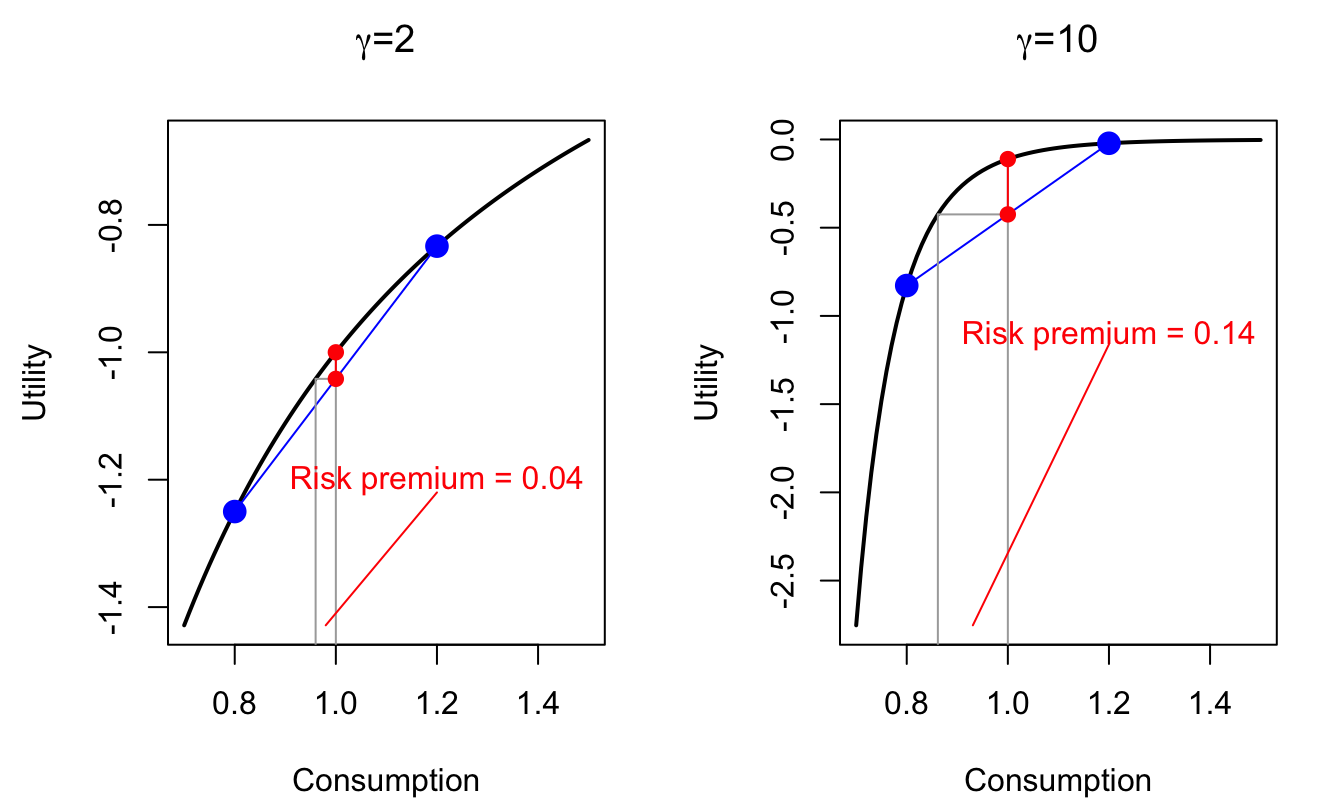
\includegraphics[width=0.95\linewidth]{TSM_files/figure-latex/RRAIESCCAPM-1} \caption{Power utility situation. Illustration of the RRA or the IES.}\label{fig:RRAIESCCAPM}
\end{figure}

\end{example}

\begin{example}[A practical interpretation of the RRA]
\protect\hypertarget{exm:CCAPMRRAinvestment}{}\label{exm:CCAPMRRAinvestment}Consider an agent whose wealth is \(W\). She will consumes only on date \(1\), and features a power utility function \(U\) (see Example \ref{exm:CCAPM}). She can invest, on date \(0\), in an asset whose price is 1 and whose payoff is \(1+\varepsilon\) with probability \(1/2\) and \(1/(1+\varepsilon)\) with probability \(1/2\).

We want to compute the optimal share of wealth, denoted by \(\alpha\), invested in the asset. The expected utility is:
\[
\frac{1}{2}U\left(C(1-\alpha)+C\alpha(1+\varepsilon)\right) + \frac{1}{2}U\left(C(1-\alpha)+C\alpha/(1+\varepsilon)\right).
\]
Taking the second-order Taylor expansion of the previous expression and letting \(\varepsilon\) tend to zero, it appears that one has to maximize the following expression:
\[
\alpha U'(C) + \frac{1}{2}C \alpha^2 U''(C).
\]
Hence, the utility is maximized for:
\[
\alpha = - \frac{U'(C)}{C U''(C)} = \frac{1}{RRA}.
\]
\end{example}

The CCAPM is a simple model; it is easy to test once a form for \(u\) has been posited. It turns out it is difficult to reconcile with the data (see next subsection).

\hypertarget{the-limitations-of-the-ccapm}{%
\subsection{The limitations of the CCAPM}\label{the-limitations-of-the-ccapm}}

Three important limitations of the CCAPM approach have been largely documented in the literature:

\begin{itemize}
\tightlist
\item
  Fitting average excess return implies implausible risk aversions (\emph{equity premium puzzle}).
\item
  The resulting risk-free short-term rate is too large unless risk aversion is small (\emph{interest-rate puzzle}).
\item
  It suggests maximum Sharpe ratios that are far too low \citep{Hansen_Jagannathan_1991}.
\end{itemize}

Using Eq. \eqref{eq:MRCov} in the power-utility situation, we get the following average excess return:
\begin{eqnarray*}
\mathbb{E}_t(R_{i,t+1} - R_{f,t}) &=& - (1 + R_{f,t}) \mathbb{C}ov_t\left(\delta \dfrac{u'(C_{t+1})}{u'(C_{t})},R_{i,t+1}\right)\\
&\approx& (1 + R_{f,t}) \delta \gamma  \mathbb{C}ov_t\left(\Delta c_{t+1},R_{i,t+1}\right),
\end{eqnarray*}
where \(\Delta c_{t+1} = \log(C_{t+1}/C_t)\).
Because consumption is smooth, the covariance \(\mathbb{C}ov_t\left(\Delta c_{t+1},R_{i,t+1}\right)\) is relatively small.
Hence, in order to replicate large average excess return, \(\gamma\) has to be big (see last two columns of the following table, from \citet{Campbell_1999}).

\begin{figure}

{\centering 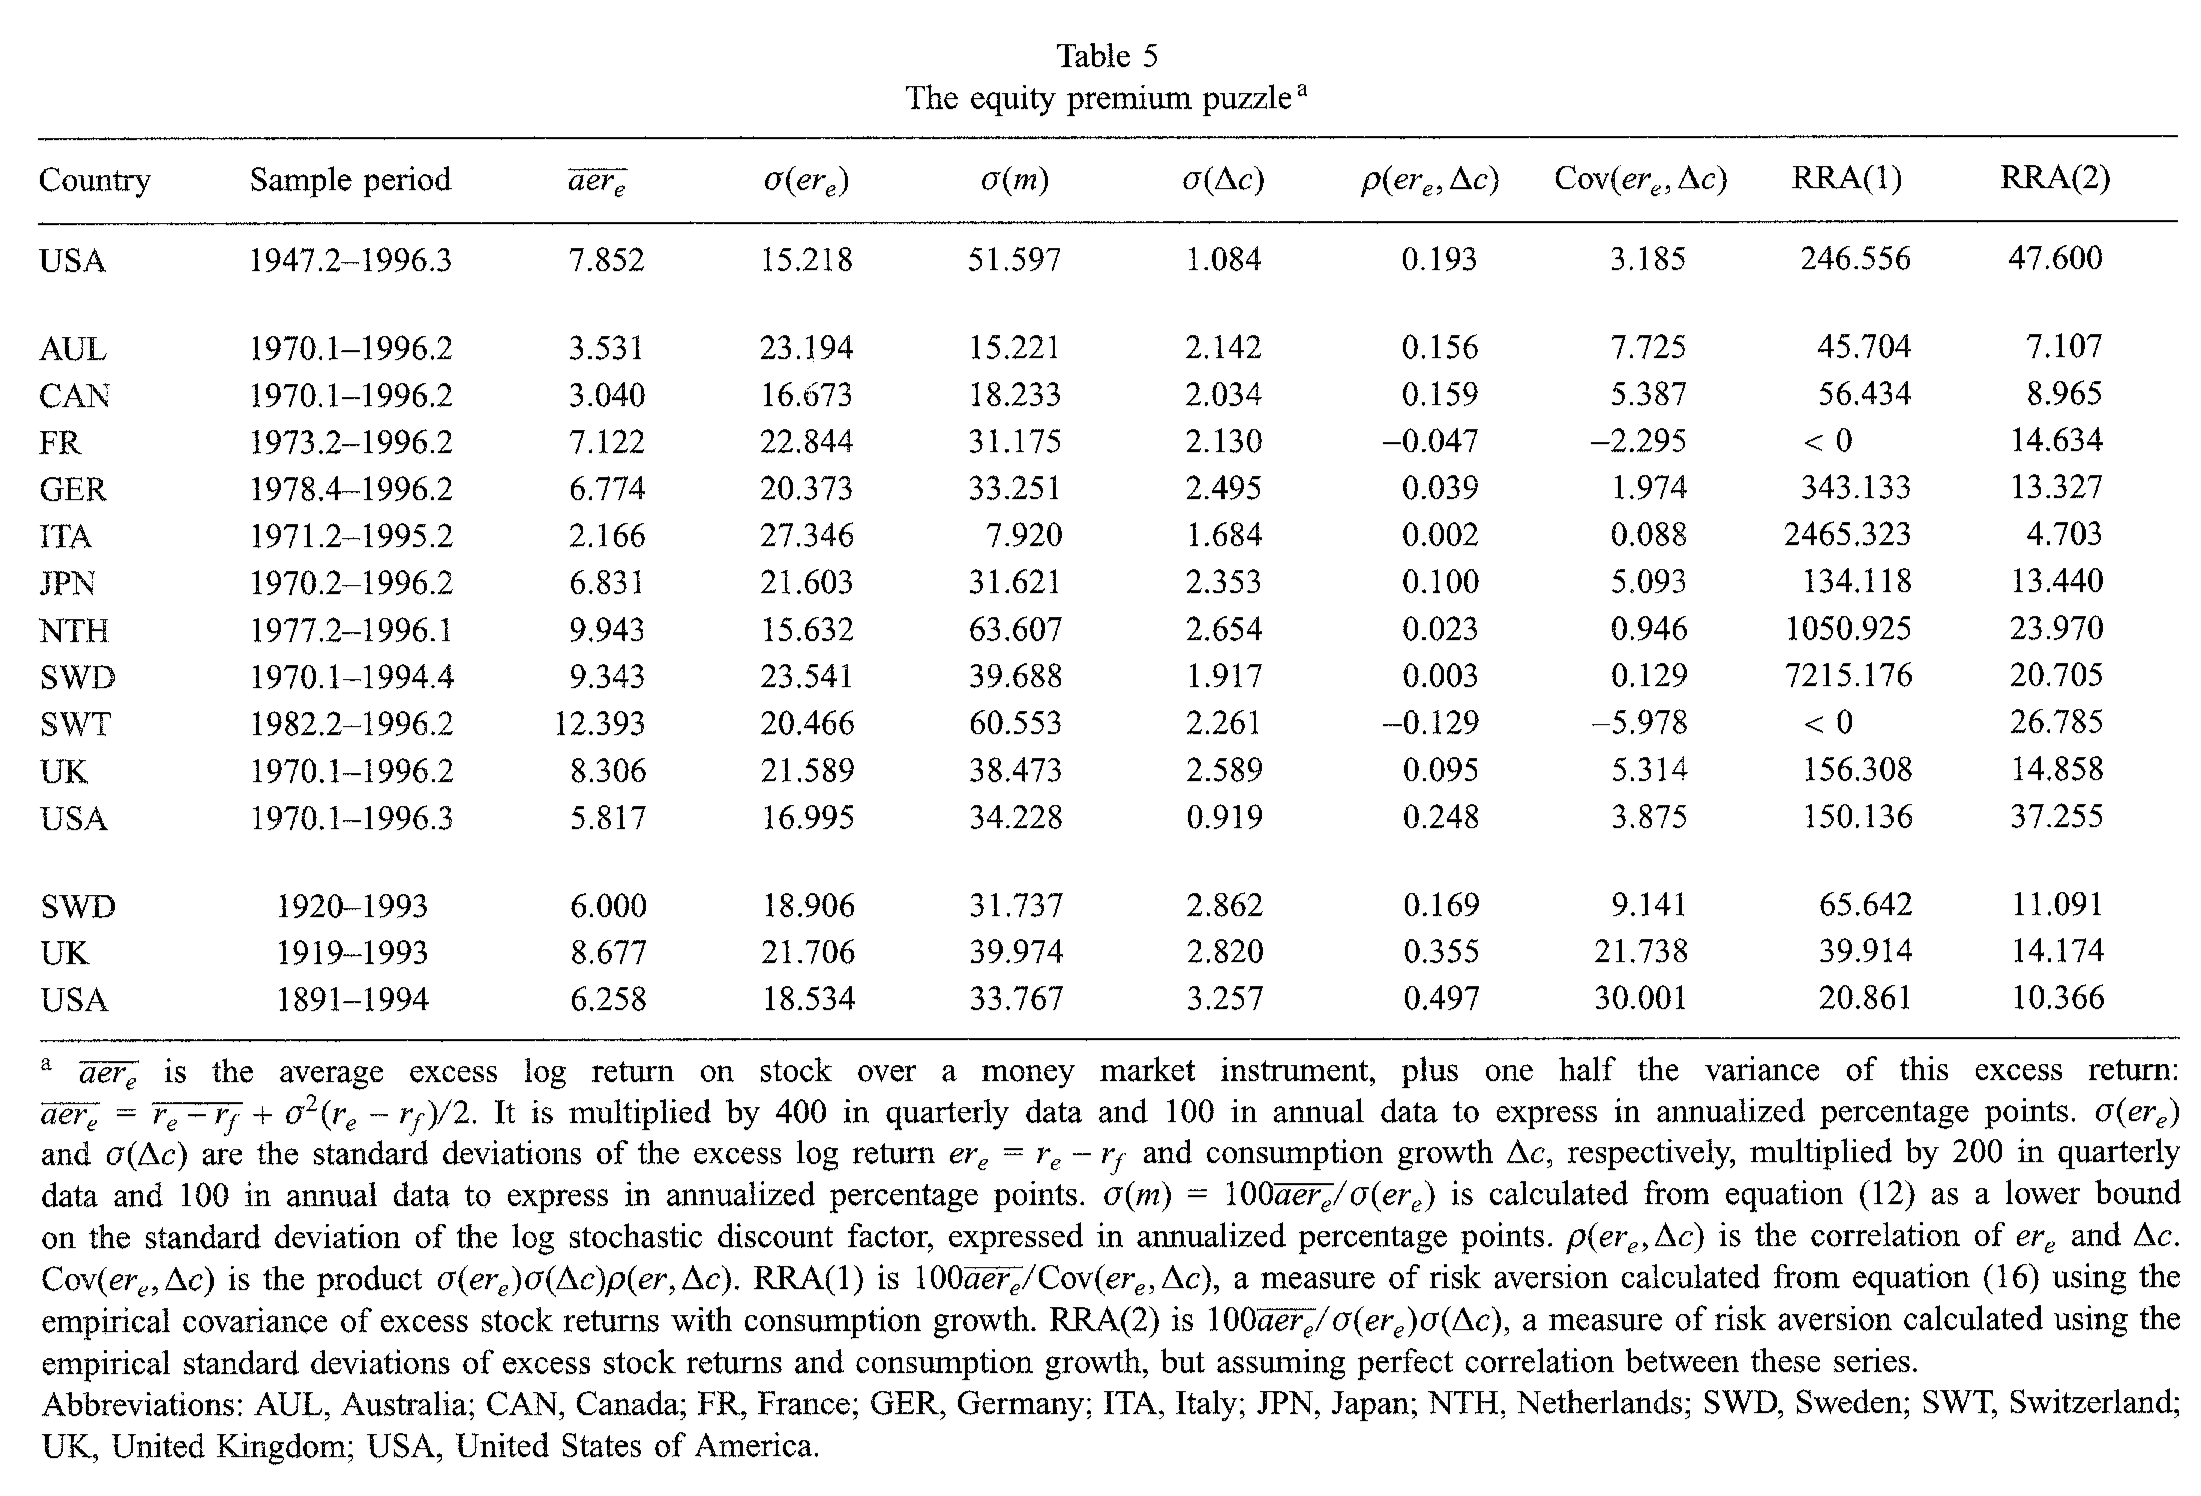
\includegraphics[width=1\linewidth]{figures/table_campbell1999_eqpuzzle} 

}

\caption{Source: Campbell (1999).}\label{fig:Campbell1}
\end{figure}

For sake of comparison: microeconomic study points to estimates of \(\gamma\) in \([1,3]\) (e.g., \citet{Hartley_Lanot_Walker_2014}). This constitutes the \emph{equity premium puzzle} \citep{Mehra_Prescott_1985}.

What if one uses a high risk aversion to get high enough risk premiums? In that case, a novel problem arise \citep{Kandel_Stambaugh_1991}: If people are very risk averse, they want to transfer consumption from high levels to low levels.
In order to allow for a 2\% average increase in \(C_t\), the model predicts that average short-term rate should be high (to prevent people from borrowing too much). Such high interest rates are at odds with the data. This is the \emph{risk-free rate puzzle}.

In the case of the power utility function, the risk aversion is the inverse of the Intertemporal Elasticity of Substitution (Def. \ref{def:IES}):
\[
\mbox{High risk aversion} \Leftrightarrow \mbox{Low IES}.
\]
For given values of the risk-free rates \(R_{f,t}\), a decrease in the IES (increase in \(\gamma\)) leads people to make consumption smoother (see Example \ref{exm:IESsmooth}).
\[
\frac{1}{1+R_{f,t}} \approx \mathbb{E}_t(\delta (1 - \gamma \Delta c_{t+1}))
\]
Consequently, for the very large \(\gamma\) values needed to adjust average excess returns on equities, agents have a strong desire to smooth consumption. To reconcile a high risk aversion this with the observed low real interest rate observed on average, it must be that investors are infinitely patients (\emph{risk-free rate puzzle}):
If \(\gamma=10\), \(R_{f,t} \approx 0\%\) and \(\Delta c_{t+1} \approx 2\%\), then \(\delta \approx 1.25\), which is not reasonable.

\begin{example}[IES and smoothing behavior]
\protect\hypertarget{exm:IESsmoothing}{}\label{exm:IESsmoothing}

The agents have a wealth of 1 unit that they consume over two periods. If they consume \(C_1\) in period, they consume \((1+R)(1-C_1)\) in period 2. They feature power-utility time-separable preferences with \(\delta=1\) and \(R=5\%\).

The optimization of the intertemporal utility of the agents imply that \(1/(1+R)=(C_2/C_1)^{-\gamma}\). Hence, the lower the IES, the smoother the consumption path.

\begin{figure}
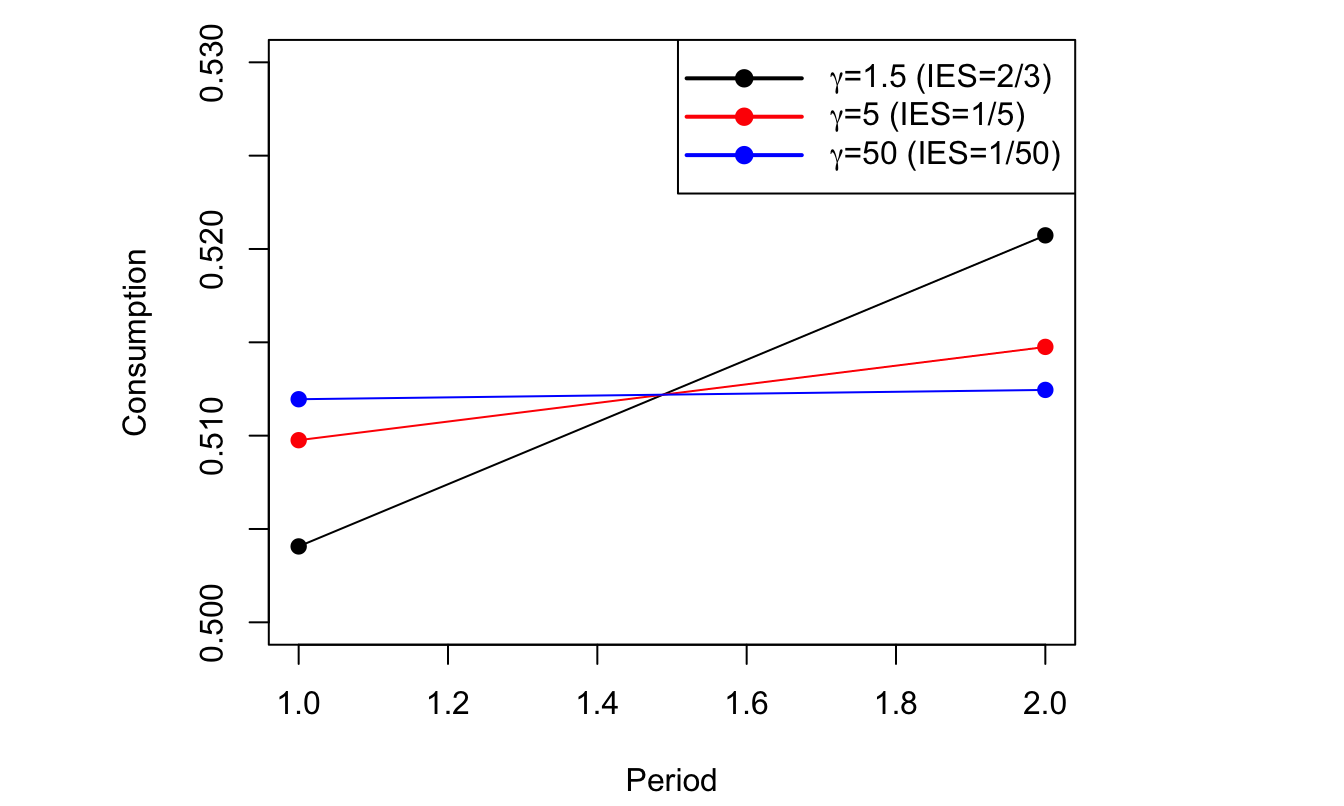
\includegraphics[width=0.95\linewidth]{TSM_files/figure-latex/IESsmooth-1} \caption{Power utility situation. IES and consumption smoothing.}\label{fig:IESsmooth}
\end{figure}

\end{example}

A third problem pertains to the volatility of the SDF. \citet{Grossman_Shiller_1981} and \citet{Hansen_Jagannathan_1991} show that observed Sharpe ratios give lower bounds to the volatility of SDF:
\[
\frac{\sigma_t(\mathcal{M}_{t,t+1})}{\mathbb{E}_t(\mathcal{M}_{t,t+1})} \ge \underbrace{\frac{\mathbb{E}_t(R_{i,t+1}-R_{f,t})}{\sigma_t(R_{i,t+1})}}_{\mbox{Sharpe ratio of asset $i$.}}
\]
The previous inequality results from Eq. \eqref{eq:MRCov}, using the fact that \(\mathbb{C}ov(X,Y) \le \sigma(X)\sigma(Y)\).

For postwar U.S. stock market, the Sharpe ratio is about 50\% see Table \ref{fig:Campbell1}). Given that \(\mathbb{E}_t(\mathcal{M}_{t,t+1}) \approx 1\), this implies that the volatility of the SDF should be at least 50\%.
However, for a power utility function:
\[
\mathcal{M}_{t,t+1}=\delta (C_t/C_{t+1})^\gamma \approx (1 - \gamma \Delta c_{t+1}).
\]
Given the small volatility of \(\Delta c_{t+1}\) (see column \(\sigma(\Delta c)\) in Table \ref{fig:Campbell1}, or use this \href{https://jrenne.shinyapps.io/APModels}{web interface}), \(\gamma\) should be very high for the SDF volatility to be equal to 50\%.

\begin{example}[Econometric Test of the C-CAPM: the GMM approach]
\protect\hypertarget{exm:GMM}{}\label{exm:GMM}

\citet{Hansen_Singleton_1982} have developed and used the General Method of Moments to test the C-CAPM. This approach is based on Eq. \eqref{eq:pricingcapm}:
\begin{equation}
1 = \color{red}{\mathbb{E}_t}\left( \delta \left(\frac{C_t}{C_{t+1}}\right)^\gamma (1+R_{i,t+1})\right).\label{eq:momentcondi}
\end{equation}
For this to be verified, we must have, for any variable \(z_t\):
\begin{equation}
\color{red}{\mathbb{E}}\left( \underbrace{\left[\delta \left(\frac{C_t}{C_{t+1}}\right)^\gamma (1+R_{i,t+1}) - 1\right] z_t}_{h_{t+1}}\right) = 0,\label{eq:GMM}
\end{equation}
If this is not the case, one can use \(z_t\) to predict \(\delta \left(\frac{C_t}{C_{t+1}}\right)^\gamma (1+R_{i,t+1})\) and Eq. \eqref{eq:momentcondi} is not valid. Moment condition: \(\mathbb{E}(h_{t+1})=0\).

Empirical counterpart of the moment condition \eqref{eq:GMM}:
\begin{equation}
\frac{1}{T}\sum_{t=1}^{T} \left[\hat\delta \left(\frac{C_t}{C_{t+1}}\right)^{\hat\gamma} (1+R_{i,t+1}) - 1\right] \times\underbrace{z_{j,t}}_{\mbox{instrument}} = 0.
\end{equation}
In order to identify \(\delta\) and \(\gamma\), one need at least two such equations (with some \(z_{1,t}\) and \(z_{2,t}\)). \citet{Hansen_Singleton_1982} used lagged values of \(R_{i,t+1}\) as instruments. {[}New York Stock Exchange indexes + indexes for different industries{]}

If we have more than two equations, we are in a situation of over-identification. One can use over-identifying restrictions to test for the model.

THey obtained economically meaningful estimates with \(\gamma\) (\(=-\hat\alpha\) in the table below) close to unity (although with a large standard error) and \(\delta\) (\(=\hat\beta\) in the table below) slightly smaller than unity. However, when applied to more than one stock index, the over-identifying restrictions are generally rejected. The data reject the simple version of CCAPM.

\begin{figure}

{\centering 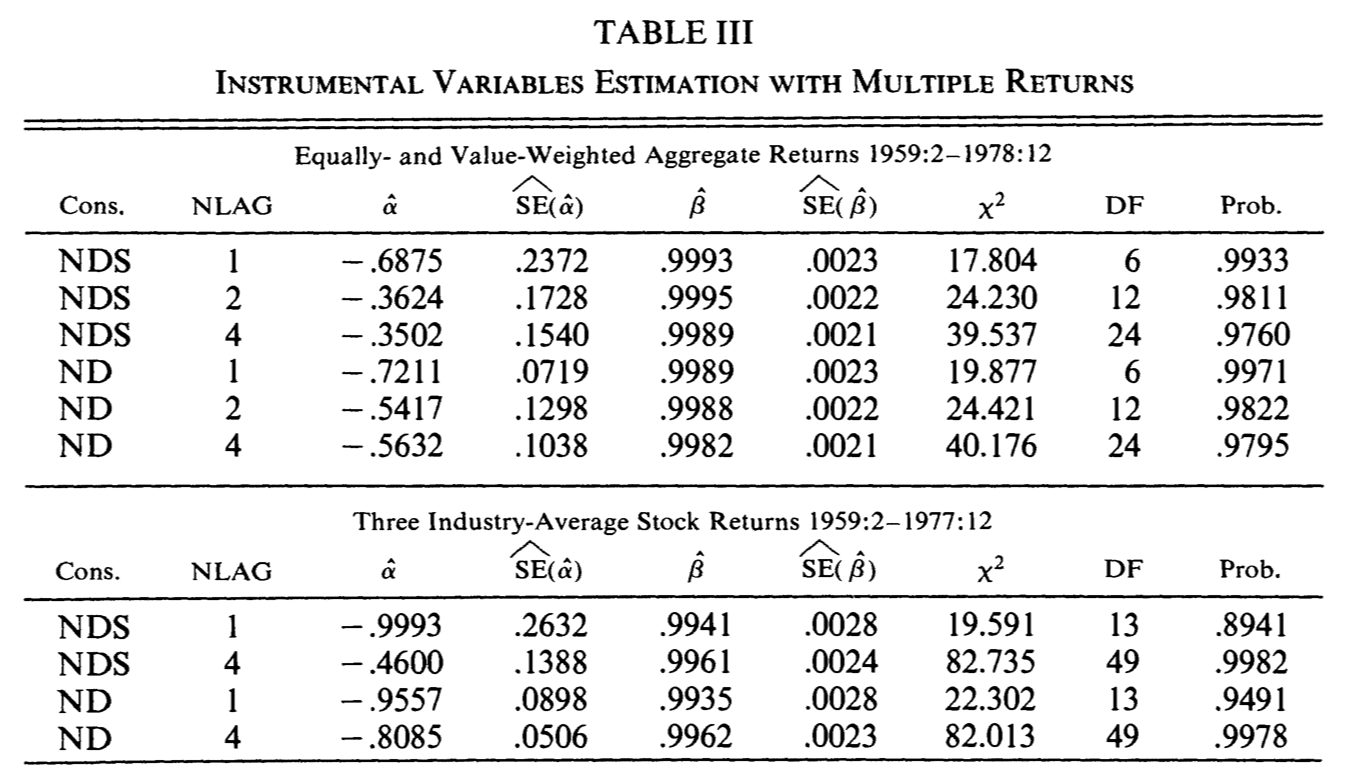
\includegraphics[width=1\linewidth]{figures/tableHansenSingleton82A} 

}

\caption{Source: Hansen and Singleton (1982).}\label{fig:HansenSinfgleton1982}
\end{figure}

\end{example}

\hypertarget{c-capm-that-bad}{%
\subsection{C-CAPM: That bad?}\label{c-capm-that-bad}}

Some studies show that the CCAPM-based puzzles are somehow alleviated when considering longer investment horizons. Indeed, stocks and consumption are more correlated at low frequencies (see, e.g., this \href{https://jrenne.shinyapps.io/APModels}{web interface}). Hence equity-premium puzzle a little less strong for longer horizons (e.g., \citet{DANIEL_MARSHALL_1997}). \citet{Jagannathan_Wang_2007} find that the CCAPM performs reasonably well when using fourth-quarter over fourth-quarter non-durable and service consumption. \citet{Parker_Julliard_2005} study whether the 25 Fama-French portfolios can be priced when considering their exposure to ``long-run'' consumption risk, and find better results than in the standard situation.

According to \citet{Cochrane_2005}, the failure of the C-CAPM models is quantitative, not qualitative. In particular:

\begin{itemize}
\tightlist
\item
  The signs are consistent: since stock market returns are positively correlated with consumption growth, the premiums must be positive (which they are).
\item
  The decrease in bond term premiums over the last decades is consistent with decrease in the correlation between long-term bond excess returns and consumption (see Figure \ref{fig:fredCorrel}, and this \href{https://jrenne.shinyapps.io/APModels}{web interface}).
\item
  In terms of signs, the CAPM is also consistent with currency risk premiums.\footnote{\citet{Lustig_Verdelhan_2007} show that high interest rate currencies depreciate on average when domestic consumption growth is low \(\Rightarrow\) the CAPM predicts higher average return for investments in foreign high-interest rate currencies.}
\end{itemize}

\begin{figure}
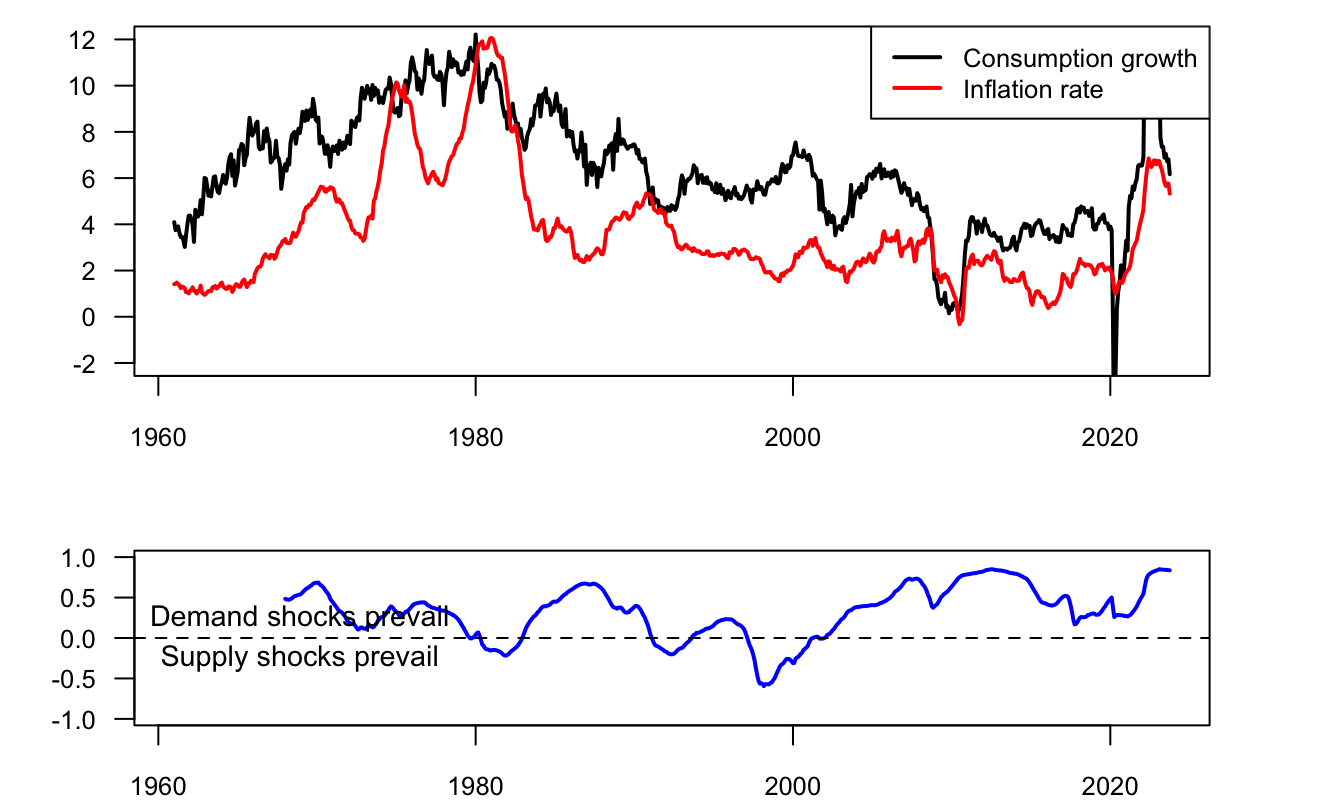
\includegraphics[width=0.95\linewidth]{TSM_files/figure-latex/fredCorrel-1} \caption{Consumption-Inflation correlation. Growth rates are 2-year growth rates. Dynamic correlation is computed using a 7-year rolling window.}\label{fig:fredCorrel}
\end{figure}

\hypertarget{the-term-structure-of-real-interest-rates-in-the-ccapm}{%
\subsection{The term structure of real interest rates in the CCAPM}\label{the-term-structure-of-real-interest-rates-in-the-ccapm}}

Consider the following AR(1) process for \(g_t\) (\(=\Delta c_{t}\)):
\[
g_{t+1} = \mu + \phi (g_t - \mu) + \sigma_c \varepsilon_{c,t+1},\quad \varepsilon_{c,t} \sim i.i.d.\mathcal{N}(0,1).
\]

Let's denote by \(r_{f,t}\) the one-period risk-free real interest rate.

Applying \eqref{eq:SDF100} to the one-period risk-free real bond, using that the real SDF, between dates \(t\) and \(t+1\), is given by \(\delta\exp(-\gamma \Delta c_{t,t+1})\), we get:
\begin{eqnarray*}
P_{t,1} = \exp(-r_{f,t}) &=& \mathbb{E}_t \left[ \delta \exp(-\gamma \Delta c_{t+1}) \underbrace{\times 1}_{= x_{i,t+1}} \right]\\
&=& \delta \exp\left(-\gamma(\mu + \phi (g_t - \mu))+\frac{\gamma^2\sigma_c^2}{2}\right).
\end{eqnarray*}
As a result, the short-term real rate is given by
\begin{equation}
r_{f,t} = \underbrace{- \log(\delta) + \gamma \mu (1-\phi)  - \frac{\gamma^2\sigma_c^2}{2}}_{=\eta_0} + \underbrace{\gamma \phi}_{=\eta_1} g_t.\label{eq:rCCAPM}
\end{equation}
To price longer-term real bonds, one can use Eq. \eqref{eq:SDF100} iteratively. For instance, for \(h=2\):
\begin{eqnarray*}
P_{t,2} &=&  \mathbb{E}_t \left[ \delta \exp(-\gamma \Delta c_{t+1}) \color{blue}{P_{t+1,1}} \right]\\
&=& \mathbb{E}_t \big[ \delta \exp(-\gamma \Delta c_{t+1}) \color{blue}{\mathbb{E}_{t+1} \big[ \delta \exp(-\gamma \Delta c_{t+2}) \underbrace{\times 1}_{=P_{t+2,0}} \big]} \big]\\
&=& \mathbb{E}_t \left[ \delta^2 \exp(-\gamma \Delta c_{t+1} - \gamma \Delta c_{t+2}) \right].
\end{eqnarray*}
Further, for \(h>1\):
\begin{equation}
P_{t,h} = \mathbb{E}_t \left[ \delta^h \exp(-\gamma \Delta c_{t+1} - \gamma \Delta c_{t+2} \dots - \gamma \Delta c_{t+h}) \right].\label{eq:PthCCAPM}
\end{equation}
It is then tempting to say that this price is also equal to
\begin{equation}
\mathbb{E}_t \left[ \exp(- r_{f,t} - r_{f,t+1} - \dots - r_{f,t+h-1}) \right],\label{eq:CCAPMEH}
\end{equation}
but this is not true. This would be the case under the expectation hypothesis (see Eq. \eqref{eq:stdbondRFchapterP}).

Take \(P_{t,2}\). We have seen that:
\begin{eqnarray*}
P_{t,2} &=&  \mathbb{E}_t \left[ \delta \exp(-\gamma \Delta c_{t+1}) \color{blue}{P_{t+1,1}} \right]\\
&=& \mathbb{E}_t \left[ \delta \exp(-\gamma \Delta c_{t+1}) \color{blue}{\exp(- r_{f,t+1})} \right].
\end{eqnarray*}
Since \(r_{f,t+1}\) and \(\Delta c_{t+1}\) are correlated, we have that \(\mathbb{C}ov(\exp(-\gamma \Delta c_{t+1}),\exp(- r_{f,t+1}))\ne 0\), and:
\begin{eqnarray*}
&&\mathbb{E}_t \left[ \delta \exp(-\gamma \Delta c_{t+1}) \exp(- r_{f,t+1}) \right]\\
&=& \underbrace{\mathbb{E}_t \left[ \delta \exp(-\gamma \Delta c_{t+1}) \right]}_{=\exp(-r_{f,t})}\mathbb{E}_t \left[ \exp(- r_{f,t+1}) \right] + \mathbb{C}ov(\exp(-\gamma \Delta c_{t+1}),\exp(- r_{f,t+1}))\\
&=& \mathbb{E}_t \left[ \exp(- r_{f,t}- r_{f,t+1}) \right] + \underbrace{\mathbb{C}ov(\exp(-\gamma \Delta c_{t+1}),\exp(- r_{f,t+1}))}_{\ne 0}\\
&\ne& \mathbb{E}_t \left[ \exp(- r_{f,t}- r_{f,t+1}) \right].
\end{eqnarray*}
The covariance term gives rise to term premiums. This is illustrated by Figure \ref{fig:TSMCCAPM}. Note that the (real) term premiums are negative, which is typical in the context of equilibrium term structure models \citep{Piazzesi_Schneider_2007}. Indeed, in these models, it is often that case that \(\Delta c_{t+1}\) and \(r_{f,t+1}\) are positively correlated, which implies here that \(R_{t,2} < R_{t,2}^{EH}\).

Exploiting the fact that the state variable (\(g_t\)) follows an affine process, Proposition \ref{prp:reverseMLT} can be used to recursively compute the bond prices given in \eqref{eq:PthCCAPM}. These prices are exponential affine in \(g_t\), and the real rates are therefore affine functions of \(g_t\).

In order to compute the counterfactual yields that would prevail under the Expectation Hypothesis, we also make use of the Proposition \ref{prp:reverseMLT}. Specifically, we have (from Eq. \eqref{eq:CCAPMEH}):
\begin{eqnarray}
R^{EH}_{t,h} &=& -\frac{1}{h} \log \mathbb{E}_t \left[ \exp(- r_{f,t} - r_{f,t+1} - \dots - r_{f,t+h-1}) \right] \\
&=& \eta_0 -\frac{1}{h} \log \mathbb{E}_t \left[ \exp(  - \eta_1 g_{t+1} - \dots - \eta_1 g_{t+h-1}) \right],
\end{eqnarray}
where \(\eta_0\) and \(\eta_1\) are defined in \eqref{eq:rCCAPM}.

\begin{Shaded}
\begin{Highlighting}[]
\FunctionTok{library}\NormalTok{(AEC);}\FunctionTok{library}\NormalTok{(TSModels)}
\NormalTok{phi }\OtherTok{\textless{}{-}} \FloatTok{0.6}\NormalTok{;mu }\OtherTok{\textless{}{-}} \FloatTok{0.01}
\NormalTok{sigma.bar }\OtherTok{\textless{}{-}}\NormalTok{ .}\DecValTok{01} \CommentTok{\# unconditional std dev of growth}
\NormalTok{sigma2  }\OtherTok{\textless{}{-}}\NormalTok{ sigma.bar}\SpecialCharTok{\^{}}\DecValTok{2} \SpecialCharTok{*}\NormalTok{ (}\DecValTok{1} \SpecialCharTok{{-}}\NormalTok{ phi}\SpecialCharTok{\^{}}\DecValTok{2}\NormalTok{)}
\NormalTok{sigma.c }\OtherTok{\textless{}{-}} \FunctionTok{sqrt}\NormalTok{(sigma2)}
\NormalTok{gamma   }\OtherTok{\textless{}{-}} \DecValTok{10}
\NormalTok{delta   }\OtherTok{\textless{}{-}} \FloatTok{0.99}
\CommentTok{\# Determine specification of real short{-}term rate:}
\NormalTok{eta}\FloatTok{.0} \OtherTok{\textless{}{-}} \SpecialCharTok{{-}}\FunctionTok{log}\NormalTok{(delta) }\SpecialCharTok{+}\NormalTok{ mu }\SpecialCharTok{*}\NormalTok{ gamma }\SpecialCharTok{*}\NormalTok{ (}\DecValTok{1} \SpecialCharTok{{-}}\NormalTok{ phi) }\SpecialCharTok{{-}}\NormalTok{ gamma}\SpecialCharTok{\^{}}\DecValTok{2} \SpecialCharTok{*}\NormalTok{ sigma.c}\SpecialCharTok{\^{}}\DecValTok{2} \SpecialCharTok{/} \DecValTok{2}
\NormalTok{eta}\FloatTok{.1} \OtherTok{\textless{}{-}}\NormalTok{ gamma }\SpecialCharTok{*}\NormalTok{ phi}
\CommentTok{\# Specify the model:}
\NormalTok{psi.parameterization }\OtherTok{\textless{}{-}} \FunctionTok{list}\NormalTok{(}
  \AttributeTok{mu =} \FunctionTok{matrix}\NormalTok{(mu }\SpecialCharTok{*}\NormalTok{ (}\DecValTok{1}\SpecialCharTok{{-}}\NormalTok{phi)),}
  \AttributeTok{Phi =} \FunctionTok{matrix}\NormalTok{(phi),}
  \AttributeTok{Sigma =} \FunctionTok{matrix}\NormalTok{(sigma.c}\SpecialCharTok{\^{}}\DecValTok{2}\NormalTok{))}
\CommentTok{\# Use reverse{-}order multi{-}horizon LT to price ZC bonds:}
\NormalTok{h }\OtherTok{=} \DecValTok{10} \CommentTok{\# maximum maturity}
\NormalTok{u2 }\OtherTok{\textless{}{-}} \FunctionTok{matrix}\NormalTok{(}\SpecialCharTok{{-}}\NormalTok{gamma)}
\NormalTok{u1 }\OtherTok{\textless{}{-}} \FunctionTok{matrix}\NormalTok{(}\SpecialCharTok{{-}}\NormalTok{gamma)}
\NormalTok{AB }\OtherTok{\textless{}{-}} \FunctionTok{reverse.MHLT}\NormalTok{(psi.GaussianVAR,u1,u2,}\AttributeTok{H=}\NormalTok{h,psi.parameterization)}
\NormalTok{a.h }\OtherTok{\textless{}{-}} \SpecialCharTok{{-}}\FunctionTok{c}\NormalTok{(AB}\SpecialCharTok{$}\NormalTok{A)}\SpecialCharTok{/}\NormalTok{(}\DecValTok{1}\SpecialCharTok{:}\NormalTok{h)}
\NormalTok{b.h }\OtherTok{\textless{}{-}} \SpecialCharTok{{-}} \FunctionTok{log}\NormalTok{(delta) }\SpecialCharTok{+} \SpecialCharTok{{-}}\FunctionTok{c}\NormalTok{(AB}\SpecialCharTok{$}\NormalTok{B)}\SpecialCharTok{/}\NormalTok{(}\DecValTok{1}\SpecialCharTok{:}\NormalTok{h)}
\CommentTok{\# Under EH:}
\NormalTok{u2 }\OtherTok{\textless{}{-}} \FunctionTok{matrix}\NormalTok{(}\SpecialCharTok{{-}}\NormalTok{ eta}\FloatTok{.1}\NormalTok{)}
\NormalTok{u1 }\OtherTok{\textless{}{-}} \FunctionTok{matrix}\NormalTok{(}\DecValTok{0}\NormalTok{)}
\NormalTok{AB }\OtherTok{\textless{}{-}} \FunctionTok{reverse.MHLT}\NormalTok{(psi.GaussianVAR,u1,u2,}\AttributeTok{H=}\NormalTok{h,psi.parameterization)}
\NormalTok{a.h.EH }\OtherTok{\textless{}{-}} \SpecialCharTok{{-}}\FunctionTok{c}\NormalTok{(AB}\SpecialCharTok{$}\NormalTok{A }\SpecialCharTok{{-}}\NormalTok{ eta}\FloatTok{.1}\NormalTok{)}\SpecialCharTok{/}\NormalTok{(}\DecValTok{1}\SpecialCharTok{:}\NormalTok{h)}
\NormalTok{b.h.EH }\OtherTok{\textless{}{-}}\NormalTok{ eta}\FloatTok{.0} \SpecialCharTok{{-}} \FunctionTok{c}\NormalTok{(AB}\SpecialCharTok{$}\NormalTok{B)}\SpecialCharTok{/}\NormalTok{(}\DecValTok{1}\SpecialCharTok{:}\NormalTok{h)}
\CommentTok{\# Simulate growth:}
\NormalTok{x.sim }\OtherTok{\textless{}{-}} \FunctionTok{sim.arma}\NormalTok{(mu}\SpecialCharTok{*}\NormalTok{(}\DecValTok{1}\SpecialCharTok{{-}}\NormalTok{phi),phi,}\AttributeTok{theta=}\FunctionTok{c}\NormalTok{(}\DecValTok{1}\NormalTok{),sigma.c,}\AttributeTok{T=}\DecValTok{100}\NormalTok{,mu,}\AttributeTok{nb.sim=}\DecValTok{1}\NormalTok{)}
\NormalTok{r.t   }\OtherTok{\textless{}{-}}\NormalTok{ (eta}\FloatTok{.0} \SpecialCharTok{+}\NormalTok{ eta}\FloatTok{.1} \SpecialCharTok{*}\NormalTok{ x.sim)}
\CommentTok{\# Prepare plots:}
\FunctionTok{par}\NormalTok{(}\AttributeTok{mfrow=}\FunctionTok{c}\NormalTok{(}\DecValTok{1}\NormalTok{,}\DecValTok{1}\NormalTok{));}\FunctionTok{par}\NormalTok{(}\AttributeTok{plt=}\FunctionTok{c}\NormalTok{(.}\DecValTok{1}\NormalTok{,.}\DecValTok{95}\NormalTok{,.}\DecValTok{2}\NormalTok{,.}\DecValTok{95}\NormalTok{))}
\FunctionTok{plot}\NormalTok{(r.t,}\AttributeTok{type=}\StringTok{"l"}\NormalTok{,}\AttributeTok{xlab=}\StringTok{"time"}\NormalTok{,}\AttributeTok{ylab=}\StringTok{""}\NormalTok{,}\AttributeTok{ylim=}\FunctionTok{c}\NormalTok{(}\FunctionTok{min}\NormalTok{(r.t),}\FunctionTok{max}\NormalTok{(r.t)}\SpecialCharTok{+}\NormalTok{.}\DecValTok{02}\NormalTok{),}\AttributeTok{las=}\DecValTok{1}\NormalTok{)}
\ControlFlowTok{for}\NormalTok{(t }\ControlFlowTok{in} \FunctionTok{seq}\NormalTok{(}\DecValTok{1}\NormalTok{,T,}\AttributeTok{by=}\DecValTok{10}\NormalTok{))\{}
  \FunctionTok{lines}\NormalTok{(t}\SpecialCharTok{+}\NormalTok{(}\DecValTok{1}\SpecialCharTok{:}\NormalTok{h)}\SpecialCharTok{{-}}\DecValTok{1}\NormalTok{,b.h    }\SpecialCharTok{+}\NormalTok{ a.h    }\SpecialCharTok{*}\NormalTok{ x.sim[t],}\AttributeTok{col=}\StringTok{"red"}\NormalTok{,}\AttributeTok{lwd=}\DecValTok{2}\NormalTok{)}
  \FunctionTok{lines}\NormalTok{(t}\SpecialCharTok{+}\NormalTok{(}\DecValTok{1}\SpecialCharTok{:}\NormalTok{h)}\SpecialCharTok{{-}}\DecValTok{1}\NormalTok{,b.h.EH }\SpecialCharTok{+}\NormalTok{ a.h.EH }\SpecialCharTok{*}\NormalTok{ x.sim[t],}\AttributeTok{col=}\StringTok{"blue"}\NormalTok{,}\AttributeTok{lwd=}\DecValTok{2}\NormalTok{)\}}
\FunctionTok{legend}\NormalTok{(}\StringTok{"topright"}\NormalTok{,}
       \FunctionTok{c}\NormalTok{(}\StringTok{"Short{-}term rate"}\NormalTok{,}\StringTok{"Term structure of real yields"}\NormalTok{,}
         \StringTok{"Term structure of real yields (without risk premiums)"}\NormalTok{),}
       \AttributeTok{lwd=}\FunctionTok{c}\NormalTok{(}\DecValTok{2}\NormalTok{),}\AttributeTok{lty=}\FunctionTok{c}\NormalTok{(}\DecValTok{1}\NormalTok{,}\DecValTok{1}\NormalTok{,}\DecValTok{1}\NormalTok{),}\AttributeTok{col=}\FunctionTok{c}\NormalTok{(}\StringTok{"black"}\NormalTok{,}\StringTok{"red"}\NormalTok{,}\StringTok{"blue"}\NormalTok{),}\AttributeTok{seg.len =} \DecValTok{4}\NormalTok{)}
\end{Highlighting}
\end{Shaded}

\begin{figure}
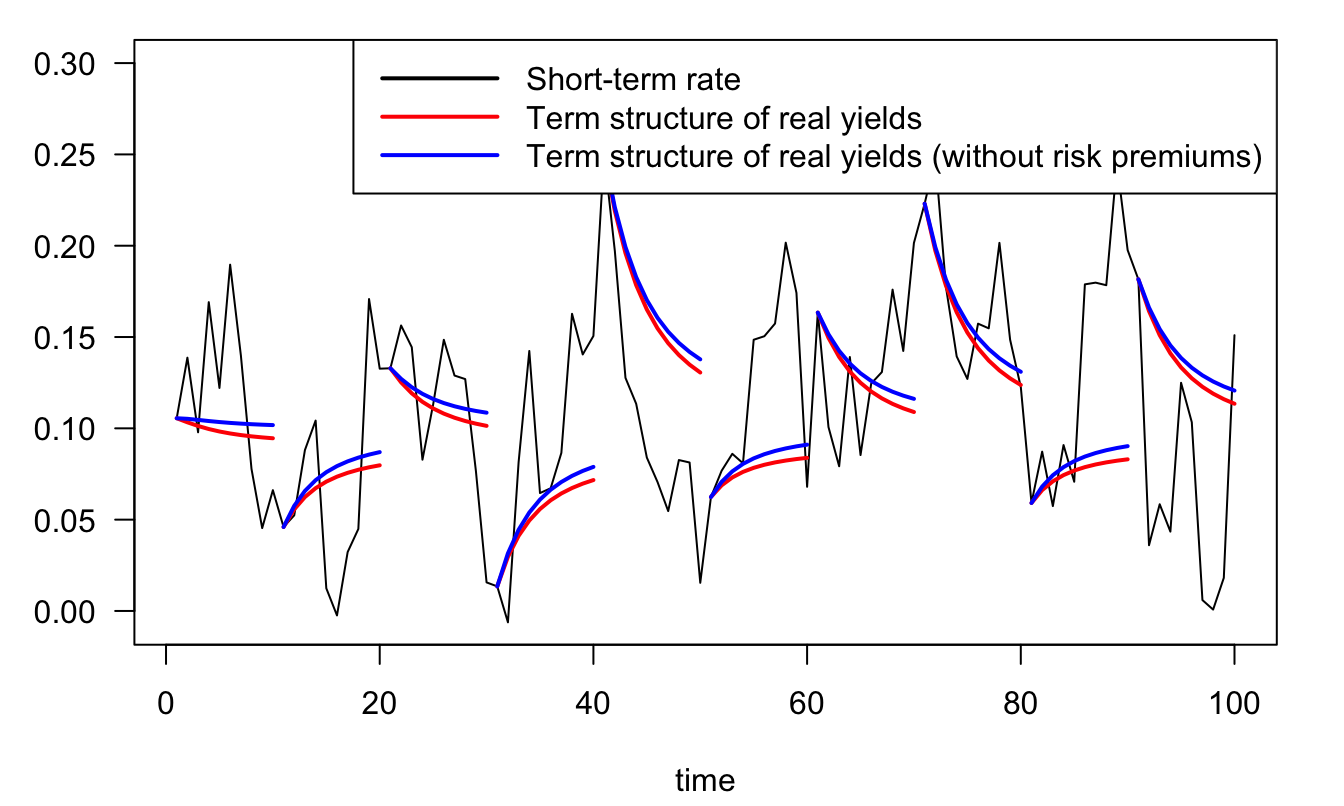
\includegraphics[width=0.95\linewidth]{TSM_files/figure-latex/TSMCCAPM-1} \caption{Term structures of real rates in a small dynamic CCAPM. The parameters are as follows: $\phi=0.6$, $\mu = 0.01$, $\gamma=10$, $\delta = 0.99$, $\sigma_c=0.008$.}\label{fig:TSMCCAPM}
\end{figure}

Let us augment this framework with inflation. Specifically, assume that:
\[
\pi_t = \mu_\pi + \phi_\pi (\pi_{t-1} - \mu_\pi) + \sigma_\pi \varepsilon_{\pi,t} + \sigma_{\pi,c}\varepsilon_{c,t},
\]
where \(\varepsilon_{\pi,t} \sim i.i.d.\,\mathcal{N}(0,1)\) is independent from \(\varepsilon_{c,t+1}\). In that framework, \(\pi_t\) and \(g_t\) are correlated; specifically:
\[
\mathbb{C}ov_t(g_{t+1},\pi_{t+1}) = \sigma_{\pi,c}\sigma_{c},
\]
whose sign is that of \(\sigma_{\pi,c}\).

The price of the nominal bond of maturity \(1\) is given by:
\begin{eqnarray*}
&&\mathbb{E}_t(\exp(\log(\delta) -\gamma \Delta c_{t+1}-\pi_{t+1}))\\
&=& \mathbb{E}_t(\exp(\log(\delta)-\gamma [\mu + \phi (g_t - \mu) + \sigma_c \varepsilon_{c,t+1}] \\
&& - \mu_\pi - \phi_\pi (\pi_{t} - \mu_\pi) - \sigma_\pi \varepsilon_{\pi,t+1} - \sigma_{\pi,c}\varepsilon_{c,t+1}))\\
&=& \exp(\log(\delta)-\gamma \mu (1-\phi) - \mu_\pi(1-\phi_\pi)-\gamma \phi g_t - \phi_\pi \pi_{t}) \times \\
&& \mathbb{E}_t(\exp( - (\gamma \sigma_c+\sigma_{\pi,c}) \varepsilon_{c,t+1}  - \sigma_\pi \varepsilon_{\pi,t+1})),
\end{eqnarray*}
which leads to the following one-period nominal interest rate:
\begin{eqnarray}
i_t &=& - \log(\delta) +\gamma \mu (1-\phi) + \mu_\pi(1-\phi_\pi) - \frac{1}{2}(\gamma \sigma_c+\sigma_{\pi,c})^2 - \frac{1}{2}\sigma_\pi^2 \nonumber\\ 
&& + \gamma \phi g_t + \phi_\pi \pi_{t}. \label{eq:nominalCCAPM}
\end{eqnarray}

The price of a nominal bond of maturity \(h\) is:
\begin{eqnarray*}
B_{t,h} &=& \mathbb{E}_t(\delta^{h}\exp(-\gamma (g_{t+1}+\dots+g_{t+h}) - \pi_{t+1}-\dots-\pi_{t+h})).
\end{eqnarray*}
This price is a multi-horizon Laplace transform of vector \(w_t = [g_t,\pi_t]'\), which follows a Gaussian VAR process:
\[
\left[\begin{array}{c}g_t\\
\pi_t\end{array}\right] = 
\left[\begin{array}{c} \mu (1-\phi)\\
\mu_\pi(1-\phi_\pi)\end{array}\right]+
\left[\begin{array}{cc} \phi & 0\\
0 & \phi_\pi\end{array}\right]\left[\begin{array}{c}g_{t-1}\\
\pi_{t-1}\end{array}\right]+
\left[\begin{array}{cc} \sigma_c & 0\\
\sigma_{\pi c} & \sigma_\pi\end{array}\right]\left[\begin{array}{c}\varepsilon_{c,t}\\
\varepsilon_{\pi,t}\end{array}\right].
\]

In the following lines of code, we use \ref{eq:} to compute the nominal yield curve. We also determine it under the Expectation Hypothesis, using \(i^{EH}_{t,h} = - \log \mathbb{E}_t [\exp(-i_t - \dots - i_{t+h-1})]\).

Figure \ref{fig:TSMCCAPM2} shows the resulting average nominal yield curves, together with the average real yield curves.

\begin{Shaded}
\begin{Highlighting}[]
\NormalTok{mu\_pi }\OtherTok{\textless{}{-}}\NormalTok{ .}\DecValTok{02}\NormalTok{;phi\_pi }\OtherTok{\textless{}{-}}\NormalTok{ .}\DecValTok{8}\NormalTok{;sigma.pi.c }\OtherTok{\textless{}{-}} \SpecialCharTok{{-}}\NormalTok{.}\DecValTok{06}\NormalTok{;sigma.pi   }\OtherTok{\textless{}{-}}\NormalTok{ .}\DecValTok{01}
\CommentTok{\# Determine specification of nominal short{-}term rate:}
\NormalTok{eta.}\FloatTok{0.}\NormalTok{i }\OtherTok{\textless{}{-}} \SpecialCharTok{{-}}\FunctionTok{log}\NormalTok{(delta) }\SpecialCharTok{+}\NormalTok{ mu }\SpecialCharTok{*}\NormalTok{ gamma }\SpecialCharTok{*}\NormalTok{ (}\DecValTok{1} \SpecialCharTok{{-}}\NormalTok{ phi) }\SpecialCharTok{+}\NormalTok{ mu\_pi }\SpecialCharTok{*}\NormalTok{ (}\DecValTok{1} \SpecialCharTok{{-}}\NormalTok{ phi\_pi) }\SpecialCharTok{{-}}
\NormalTok{  (gamma}\SpecialCharTok{*}\NormalTok{sigma.c }\SpecialCharTok{+}\NormalTok{ sigma.pi.c)}\SpecialCharTok{\^{}}\DecValTok{2}\SpecialCharTok{/}\DecValTok{2} \SpecialCharTok{{-}}\NormalTok{ sigma.pi}\SpecialCharTok{\^{}}\DecValTok{2}\SpecialCharTok{/}\DecValTok{2}
\NormalTok{eta.}\FloatTok{1.}\NormalTok{i }\OtherTok{\textless{}{-}} \FunctionTok{matrix}\NormalTok{(}\FunctionTok{c}\NormalTok{(gamma }\SpecialCharTok{*}\NormalTok{ phi,phi\_pi),}\DecValTok{2}\NormalTok{,}\DecValTok{1}\NormalTok{)}
\CommentTok{\# Specify the model:}
\NormalTok{psi.parameterization }\OtherTok{\textless{}{-}} \FunctionTok{list}\NormalTok{(}
  \AttributeTok{mu =} \FunctionTok{matrix}\NormalTok{(}\FunctionTok{c}\NormalTok{(mu}\SpecialCharTok{*}\NormalTok{(}\DecValTok{1}\SpecialCharTok{{-}}\NormalTok{phi),mu\_pi}\SpecialCharTok{*}\NormalTok{(}\DecValTok{1}\SpecialCharTok{{-}}\NormalTok{phi\_pi)),}\DecValTok{2}\NormalTok{,}\DecValTok{1}\NormalTok{),}
  \AttributeTok{Phi =} \FunctionTok{diag}\NormalTok{(}\FunctionTok{c}\NormalTok{(phi,phi\_pi)),}
  \AttributeTok{Sigma =} \FunctionTok{matrix}\NormalTok{(}\FunctionTok{c}\NormalTok{(sigma.c}\SpecialCharTok{\^{}}\DecValTok{2}\NormalTok{,sigma.c}\SpecialCharTok{*}\NormalTok{sigma.pi.c,}
\NormalTok{                   sigma.c}\SpecialCharTok{*}\NormalTok{sigma.pi.c,sigma.pi}\SpecialCharTok{\^{}}\DecValTok{2}\SpecialCharTok{+}\NormalTok{sigma.pi.c}\SpecialCharTok{\^{}}\DecValTok{2}\NormalTok{),}\DecValTok{2}\NormalTok{,}\DecValTok{2}\NormalTok{))}
\CommentTok{\# Use reverse{-}order multi{-}horizon LT to price ZC bonds:}
\NormalTok{u2 }\OtherTok{\textless{}{-}} \FunctionTok{matrix}\NormalTok{(}\FunctionTok{c}\NormalTok{(}\SpecialCharTok{{-}}\NormalTok{gamma,}\SpecialCharTok{{-}}\DecValTok{1}\NormalTok{),}\DecValTok{2}\NormalTok{,}\DecValTok{1}\NormalTok{);u1 }\OtherTok{\textless{}{-}} \FunctionTok{matrix}\NormalTok{(}\FunctionTok{c}\NormalTok{(}\SpecialCharTok{{-}}\NormalTok{gamma,}\SpecialCharTok{{-}}\DecValTok{1}\NormalTok{),}\DecValTok{2}\NormalTok{,}\DecValTok{1}\NormalTok{)}
\NormalTok{AB }\OtherTok{\textless{}{-}} \FunctionTok{reverse.MHLT}\NormalTok{(psi.GaussianVAR,u1,u2,}\AttributeTok{H=}\NormalTok{h,psi.parameterization)}
\NormalTok{a.h.i }\OtherTok{\textless{}{-}} \SpecialCharTok{{-}}\FunctionTok{matrix}\NormalTok{(AB}\SpecialCharTok{$}\NormalTok{A,}\DecValTok{2}\NormalTok{,h)}\SpecialCharTok{/}\FunctionTok{t}\NormalTok{(}\FunctionTok{matrix}\NormalTok{((}\DecValTok{1}\SpecialCharTok{:}\NormalTok{h),h,}\DecValTok{2}\NormalTok{))}
\NormalTok{b.h.i }\OtherTok{\textless{}{-}} \SpecialCharTok{{-}}\FunctionTok{log}\NormalTok{(delta) }\SpecialCharTok{+} \SpecialCharTok{{-}}\FunctionTok{c}\NormalTok{(AB}\SpecialCharTok{$}\NormalTok{B)}\SpecialCharTok{/}\NormalTok{(}\DecValTok{1}\SpecialCharTok{:}\NormalTok{h)}
\CommentTok{\# Under EH:}
\NormalTok{u2 }\OtherTok{\textless{}{-}} \FunctionTok{matrix}\NormalTok{(}\SpecialCharTok{{-}}\NormalTok{ eta.}\FloatTok{1.}\NormalTok{i);u1 }\OtherTok{\textless{}{-}} \FunctionTok{matrix}\NormalTok{(}\DecValTok{0}\NormalTok{,}\DecValTok{2}\NormalTok{,}\DecValTok{1}\NormalTok{)}
\NormalTok{AB }\OtherTok{\textless{}{-}} \FunctionTok{reverse.MHLT}\NormalTok{(psi.GaussianVAR,u1,u2,}\AttributeTok{H=}\NormalTok{h,psi.parameterization)}
\NormalTok{a.h.i.EH }\OtherTok{\textless{}{-}} \SpecialCharTok{{-}}\NormalTok{(}\FunctionTok{matrix}\NormalTok{(AB}\SpecialCharTok{$}\NormalTok{A,}\DecValTok{2}\NormalTok{,h)}\SpecialCharTok{{-}}\FunctionTok{matrix}\NormalTok{(eta.}\FloatTok{1.}\NormalTok{i,}\DecValTok{2}\NormalTok{,h))}\SpecialCharTok{/}\FunctionTok{t}\NormalTok{(}\FunctionTok{matrix}\NormalTok{((}\DecValTok{1}\SpecialCharTok{:}\NormalTok{h),h,}\DecValTok{2}\NormalTok{))}
\NormalTok{b.h.i.EH }\OtherTok{\textless{}{-}}\NormalTok{ eta.}\FloatTok{0.}\NormalTok{i }\SpecialCharTok{{-}} \FunctionTok{c}\NormalTok{(AB}\SpecialCharTok{$}\NormalTok{B)}\SpecialCharTok{/}\NormalTok{(}\DecValTok{1}\SpecialCharTok{:}\NormalTok{h)}
\CommentTok{\# Average yield curves:}
\NormalTok{avg.i.h    }\OtherTok{\textless{}{-}}\NormalTok{ b.h.i    }\SpecialCharTok{+} \FunctionTok{matrix}\NormalTok{(}\FunctionTok{c}\NormalTok{(mu,mu\_pi),}\DecValTok{1}\NormalTok{,}\DecValTok{2}\NormalTok{) }\SpecialCharTok{\%*\%}\NormalTok{ a.h.i}
\NormalTok{avg.i.h.EH }\OtherTok{\textless{}{-}}\NormalTok{ b.h.i.EH }\SpecialCharTok{+} \FunctionTok{matrix}\NormalTok{(}\FunctionTok{c}\NormalTok{(mu,mu\_pi),}\DecValTok{1}\NormalTok{,}\DecValTok{2}\NormalTok{) }\SpecialCharTok{\%*\%}\NormalTok{ a.h.i.EH}
\FunctionTok{plot}\NormalTok{(}\FunctionTok{c}\NormalTok{(avg.i.h),}\AttributeTok{type=}\StringTok{"l"}\NormalTok{,}\AttributeTok{lwd=}\DecValTok{2}\NormalTok{,}\AttributeTok{col=}\StringTok{"red"}\NormalTok{,}\AttributeTok{lty=}\DecValTok{3}\NormalTok{,}\AttributeTok{ylim=}\FunctionTok{c}\NormalTok{(}\FloatTok{0.08}\NormalTok{,}\FunctionTok{max}\NormalTok{(avg.i.h)),}
     \AttributeTok{xlab=}\StringTok{"maturity"}\NormalTok{,}\AttributeTok{ylab=}\StringTok{"yield"}\NormalTok{,}\AttributeTok{las=}\DecValTok{1}\NormalTok{);}\FunctionTok{grid}\NormalTok{()}
\FunctionTok{lines}\NormalTok{(}\FunctionTok{c}\NormalTok{(avg.i.h.EH),}\AttributeTok{type=}\StringTok{"l"}\NormalTok{,}\AttributeTok{lwd=}\DecValTok{2}\NormalTok{,}\AttributeTok{col=}\StringTok{"blue"}\NormalTok{,}\AttributeTok{lty=}\DecValTok{3}\NormalTok{)}
\FunctionTok{lines}\NormalTok{(b.h}\SpecialCharTok{+}\NormalTok{a.h}\SpecialCharTok{*}\NormalTok{mu,}\AttributeTok{lwd=}\DecValTok{2}\NormalTok{,}\AttributeTok{col=}\StringTok{"red"}\NormalTok{)}
\FunctionTok{lines}\NormalTok{(b.h.EH}\SpecialCharTok{+}\NormalTok{a.h.EH}\SpecialCharTok{*}\NormalTok{mu,}\AttributeTok{lwd=}\DecValTok{2}\NormalTok{,}\AttributeTok{col=}\StringTok{"blue"}\NormalTok{)}
\FunctionTok{legend}\NormalTok{(}\StringTok{"bottomleft"}\NormalTok{,}
       \FunctionTok{c}\NormalTok{(}\StringTok{"with risk premiums"}\NormalTok{,}
         \StringTok{"without risk premiums"}\NormalTok{),}
       \AttributeTok{lwd=}\FunctionTok{c}\NormalTok{(}\DecValTok{2}\NormalTok{),}\AttributeTok{lty=}\FunctionTok{c}\NormalTok{(}\DecValTok{1}\NormalTok{,}\DecValTok{1}\NormalTok{),}\AttributeTok{col=}\FunctionTok{c}\NormalTok{(}\StringTok{"red"}\NormalTok{,}\StringTok{"blue"}\NormalTok{),}\AttributeTok{seg.len =} \DecValTok{3}\NormalTok{)}
\end{Highlighting}
\end{Shaded}

\begin{figure}
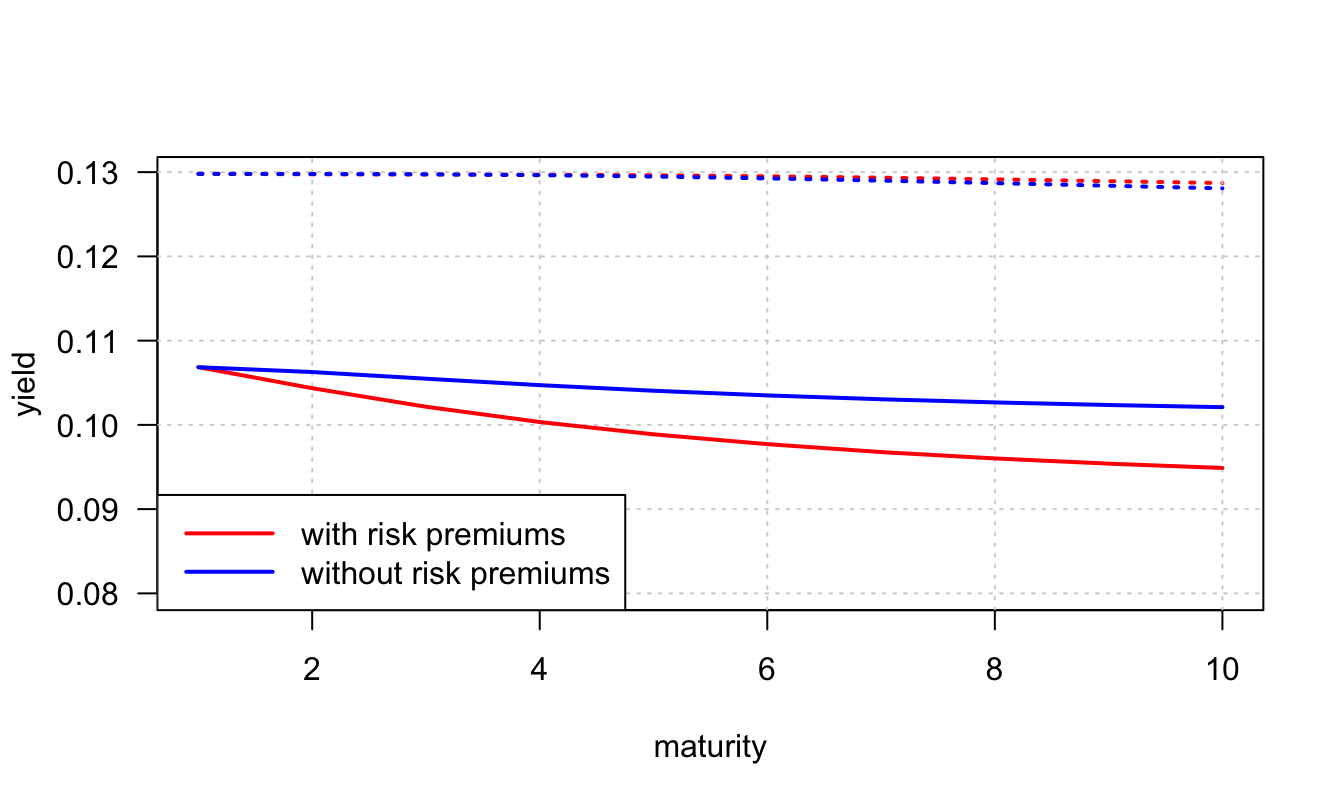
\includegraphics[width=0.95\linewidth]{TSM_files/figure-latex/TSMCCAPM2-1} \caption{Average yield curves (solid lines: real rates; dotted lines: nominal rates), using $\mu_\pi = 0.02$, $\phi_\pi=0.8$, $\sigma_{\pi,c}=-0.6$, and $\sigma_\pi=0.01$.}\label{fig:TSMCCAPM2}
\end{figure}

Using the notations used in Subsection \ref{RiskFreeGaussian}, the (nominal) SDF is of the form:
\[
\mathcal{M}_{t,t+1} = \exp(-i_t + \alpha_0'w_{t+1} - \psi_{t}(\alpha_0)),
\]
where \(\psi_t\) denotes the conditional log-Laplace transform of \(w_t\) and where \(\alpha_0 = [-\gamma,-1]'\). Therefore, according to Subsection \ref{RiskFreeGaussian}, the risk-neutral dynamics of \(w_t\) is of the form:
\[
\left[\begin{array}{c}g_t\\
\pi_t\end{array}\right] = 
\underbrace{\left[\begin{array}{c} \mu (1-\phi)\\
\mu_\pi(1-\phi_\pi)\end{array}\right]+\Sigma \lambda_0}_{=\mu^{\mathbb{Q}}}+
\left[\begin{array}{cc} \phi & 0\\
0 & \phi_\pi\end{array}\right]\left[\begin{array}{c}g_{t-1}\\
\pi_{t-1}\end{array}\right]+
\left[\begin{array}{cc} \sigma_c & 0\\
\sigma_{\pi c} & \sigma_\pi\end{array}\right]\left[\begin{array}{c}\varepsilon_{c,t}^*\\
\varepsilon_{\pi,t}^*\end{array}\right],
\]
where \(\Sigma = \left[\begin{array}{cc}\sigma_c^2&\sigma_c\sigma_{\pi,c}\\ \sigma_c\sigma_{\pi,c}&\sigma_{\pi}^2 \end{array}\right]\) and \([\varepsilon_{c,t}^*,\varepsilon_{\pi,t}^*]'\sim \mathcal{N}'^{\mathbb{Q}}(0,Id)\).

\begin{quote}
Use the risk-neutral dynamics of \(w_t\) to compute the nominal yield curve, using that \(i_{t,h} = - \log \mathbb{E}^{\mathbb{Q}}_t [\exp(-i_t - \dots - i_{t+h-1})]\).
\end{quote}

\hypertarget{recursive-utilities}{%
\section{Recursive Utilities}\label{recursive-utilities}}

Given the limitations of consumption-based models, one has questioned the utility function. But the functional form is not really an issue: in the time-separable framework, linearized and non-linearized models behave relatively similarly. (Utility functions are monotonously increasing with negative second order derivatives, so they all have the same broad shapes.) What about the arguments of the utility function? The idea is the following: the marginal utility of consumption may not depend \emph{only} on today's consumption. Pricing implications are very different when the marginal utility of consumption depends on past or (expected) future consumption. In particular, this will permit to address the following limitations of expected utility time-separable preferences (Def. \ref{def:EUTSpref}):

\begin{itemize}
\tightlist
\item
  No premium for early resolution of uncertainty: as of date \(t\), the promise to know \(C_{t+h}\) at date \(t+1\) has no value.
\item
  No utility effect of potential autocorrelation in \(C_t\): each stream of consumption intervenes independently from the others in the utility computation.
\end{itemize}

\emph{Non-separability over time} means that the marginal utility of today's consumption depends on past consumption. In other words, what you consumed yesterday can have an impact on how you feel about more consumption today.\footnote{As \citet{Cochrane_2005} puts it: ``\emph{Yesterday's pizza lowers the marginal utility for another pizza today.}'')}

\hypertarget{habit-formation}{%
\subsection{Habit formation}\label{habit-formation}}

A first example of recursive utilities is that of \emph{habit formation} \citep{Campbell_Shiller_1999}, where
\begin{equation}
U_t = \sum_{s=t}^{\infty} \delta^{s-t} u(C_s - X_s) \quad where \quad X_t = \rho X_{t-1} + \lambda C_t.\label{eq:Uhabitnonstoch}
\end{equation}

The date-\(t\) utility associated with a level of consumption \(C_t\), that is \(u(C_t - X_t)\), is lower is you already had a high level of consumption at date \(t-1\) (high \(X_t\)).
\[
U_t = \sum_{h=0}^{\infty} \delta^{h}u\left(C_{t+h} - \lambda \sum_{j=0}^\infty \rho^j C_{t+h-j}\right).
\]

A fall in consumption hurts after a few years of good times (even if the same level of consumption would have been very pleasant if it arrived after a few bad years).

If one assumes that \(X_t\) is exogenous---a case referred to as \emph{external habits}---and if \(u(Z)=Z^{1-\gamma}/(1-\gamma)\) (Def. \ref{def:power}) then:\footnote{Without the external habit assumption, the Euler equation (equilibrium relationship between risk-free short-term rate and marginal utilities) is far less tractable:
  \begin{eqnarray*}
  && 0 = \Delta U_t / \varepsilon =\\
  && \underbrace{ - u'\left(C_{t} - \lambda \sum_{j=0}^\infty \rho^j C_{t-j}\right) + \lambda  \sum_{h=0}^{\infty} \rho^h \delta^{h}u'\left(C_{t+h} - \lambda \sum_{j=0}^\infty \rho^j C_{t+h-j}\right)}_{\mbox{decrease in utility stemming from lower consumption at date $t$}} +\\
  && \underbrace{\delta(1+R_{f,t}) u'\left(C_{t+1} - \lambda \sum_{j=0}^\infty \rho^j C_{t+1-j}\right) - \lambda (1+R_{f,t}) \sum_{h=1}^{\infty} \rho^h \delta^{h}u'\left(C_{t+h} - \lambda \sum_{j=0}^\infty \rho^j C_{t+h-j}\right)}_{\mbox{increase in utility stemming from higher consumption at date $t+1$}},
  \end{eqnarray*}
  which is obtained by considering a marginal decrease in \(C_t\) by \(\varepsilon\) and an increase in \(C_{t+1}\) by \(\varepsilon(1+R_{f,t})\).}
\begin{equation}
\mathcal{M}_{t,t+1} = \delta \left( \frac{C_{t+1}}{C_t} \right)^{-\gamma}\left( \frac{S_{t+1}}{S_t} \right)^{-\gamma},\label{eq:Mhabit}
\end{equation}
where \(S_t = (C_t - X_t)/C_t\). This extends the standard power utility case by adding an additional state variable (\(X_t\)). In this model, recessions are periods where consumption is closer to habits (otherwise it is higher). SDF specifications of the type of Eq. \eqref{eq:Mhabit} can arise in more general contexts (not necessarily habits); \(S_t\) may for instance reflect a business-cycle-related variable.

\begin{example}[Comparisons of situations according to habit preferences]
\protect\hypertarget{exm:habit}{}\label{exm:habit}To illustrate, consider the following context (with no uncertainty):
\[
\delta = 1,\quad \gamma = 3, \quad \rho = 0.5, \quad \lambda = 0.49.
\]
Let's define two sequences of interest rates (A and B):
\begin{eqnarray*}
R^{(A)}_1 &=&R^{(A)}_2 =\dots=R^{(A)}_5 =  7\% \\
R^{(A)}_6 &=&R^{(A)}_7 =R^{(A)}_8 =  -20\%
\end{eqnarray*}
and
\[
R^{(B)}_1 =R^{(B)}_2 =\dots=R^{(B)}_{10} =  2.5\%.
\]
For each sequence, we compute the resulting sequence of consumption, with \(C_1=1\).
Results on next slide.

\begin{figure}
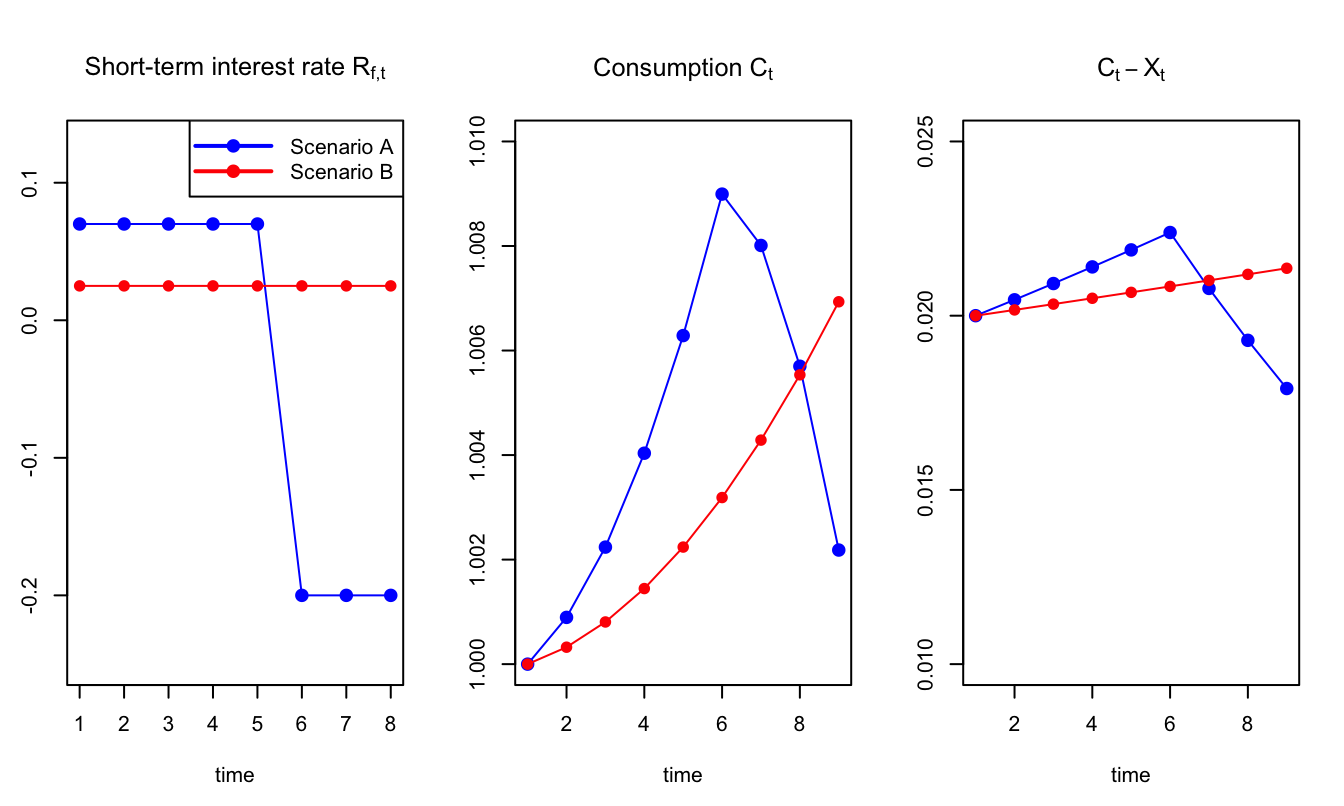
\includegraphics[width=0.95\linewidth]{TSM_files/figure-latex/Habits1-1} \caption{Comparison of scenarios A and B using habit-based preferences.}\label{fig:Habits1}
\end{figure}

The utility associated to Scenario A (\(-10779\)) is lower than that associated to Scenario B (\(-10542\)).
Without the \(X_t\) term, the utility of Scenario A would be higher than that of Scenario B.
\end{example}

\hypertarget{limitations-of-the-habit-models-for-long-horizons}{%
\subsection{Limitations of the Habit Models for Long-Horizons}\label{limitations-of-the-habit-models-for-long-horizons}}

The models based on Eq. \eqref{eq:Mhabit} generally works well in the short-run but not in the long-run. Let us consider the horizon-\(h\) SDF:
\[
\mathcal{M}_{t,t+h} = \delta \left( \frac{C_{t+h}}{C_t} \right)^{-\gamma}\left( \frac{S_{t+h}}{S_t} \right)^{-\gamma},
\]
In order to generate a high maximum Sharpe ratio for long horizons, we need a high conditional volatility of \(\mathcal{M}_{t,t+h}\).
If \(c_t\) follows a random walk, the volatility of \(\left( \frac{C_{t+h}}{C_t} \right)^{-\gamma}\) is approximately linear in \(h\).
By contrast, if \(S_t^{-\gamma}\) is stationary, then the conditional volatility of \(\left( \frac{S_{t+h}}{S_t} \right)^{-\gamma}\) does not increase indefinitely with \(h\) (though this term may substantially contribute to the short-run SDF volatility).
{[}\(\Rightarrow\){]} For long-run horizons, these models do not solve the problems pertaining to the standard power utility time-separable model.

\hypertarget{epstein-zin-preferences}{%
\subsection{Epstein-Zin preferences}\label{epstein-zin-preferences}}

\citet{Epstein_Zin_1989} have proposed a framework where there is a premium for early resolution and where the time composition of risk matters.

\begin{definition}[Epstein and Zin (1989) Preferences]
\protect\hypertarget{def:EZ}{}\label{def:EZ}Epstein-Zin preferences are defined recursively over current (known) consumption and a certainty equivalent
\(R_t(U_{t+1})\) {[}Def. \ref{def:CE}{]} of future utility:
\[
U_{t} = F(C_t,R_t(U_{t+1})),
\]
where \(R_t(U_{t+1})\), the certainty equivalent of \(U_{t+1}\), is:
\[
R_t(U_{t+1}) = G^{-1}[\mathbb{E}_t(G(U_{t+1}))],
\]
where \(F\) and \(G\) are increasing and concave functions, and where \(F\) is homogenous of degree one.
\end{definition}

\begin{quote}
We have \(R_t(U_{t+1})=\mathbb{E}_t(U_{t+1})\) if \(G\) is linear.
\end{quote}

\begin{quote}
We have \(R_t(U_{t+1})=U_{t+1}\) if \(U_{t+1}\) is not random.
\end{quote}

Standard functions \(F\) and \(G\) are (with \(\rho\) and \(\gamma\) \(>0\)):
\[
F(c,v) = \left((1-\delta)c^{1-\rho} + \delta v^{1-\rho}\right)^{\frac{1}{1-\rho}}, \quad G(x)=\frac{x^{1-\gamma}}{1-\gamma},
\]
In this case:
\begin{equation}
\boxed{ U_t = \left((1-\delta)C_t^{1-\rho}+\delta \left[\underbrace{ \mathbb{E}_t\left(U_{t+1}^{1-\gamma}\right)^{\frac{1}{1-\gamma}} }_{\mbox{certainty equivalent}}\right] ^{1-\rho}\right)^{\frac{1}{1-\rho}}.}\label{eq:EZpreferences}
\end{equation}
or
\begin{equation}
U_t = \left((1-\delta)C_t^{1-\rho} + \delta R_t(U_{t+1})^{1-\rho}\right)^{\frac{1}{1-\rho}},\label{eq:EZpreferences2}
\end{equation}
where \(R_t(U_{t+1})=\mathbb{E}_t(U_{t+1}^{1-\gamma})^{\frac{1}{1-\gamma}}\).

\begin{quote}
\textbf{Case \(\gamma = \rho\)}. If \(\gamma = \rho\), \(U_t^{1-\rho}=(1-\delta)C_t^{1-\rho} + \delta \mathbb{E}_t(U_{t+1}^{1-\rho})\).
Divide by \(1-\rho\) and replace \(U_t^{1-\rho}/(1-\rho)\) by \(W_t\). We are then back to the expected utility case {[}see Def. \ref{def:EUTSpref}{]}.
\end{quote}

\hypertarget{epstein-zin-preferences-and-risk-aversion}{%
\subsection{Epstein-Zin preferences and risk aversion}\label{epstein-zin-preferences-and-risk-aversion}}

\(\gamma\) is the \emph{relative risk aversion} {[}Def. \ref{def:RAmeasures}{]} parameter.
Consider the following context:

\begin{itemize}
\tightlist
\item
  At date 0, the agent consumes \(C_0\).
\item
  At date 1, he consumes \(C_h\) (high) with probability \(1/2\) and \(C_l\) (low) with probability \(1/2\).
\item
  In the subsequent periods, he consumes 0.
\end{itemize}

We have \(U_2 = 0\) and
\[
U_1 = U_h = (1-\delta)^{\frac{1}{1-\rho}}C_h \mbox{ with probability 1/2}
\]
and
\[
U_1 = U_l = (1-\delta)^{\frac{1}{1-\rho}}C_l \mbox{ with probability 1/2}.
\]
Therefore
\[
U_0 =  \left((1-\delta)C_0^{1-\rho} + \delta \left(\frac{1}{2}U_h^{1-\gamma}+\frac{1}{2}U_l^{1-\gamma}\right)^{\frac{1-\rho}{1-\gamma}}\right)^{\frac{1}{1-\rho}}.
\]

What is the certainty equivalent \(C_1\) to the period-1 gamble? \(C_1\) solves:
\[
U_0 = \left((1-\delta)C_0^{1-\rho} + \delta (1-\delta) C_1^{1-\rho}\right)^{\frac{1}{1-\rho}},
\]
that is:
\[
C_1 = \left(\frac{1}{2}C_h^{1-\gamma}+\frac{1}{2}C_l^{1-\gamma}\right)^{\frac{1}{1-\gamma}}.
\]
This certainty equivalent is the same as the one that one would get if the utility function was the standard (time-separable) power utility function (with RRA \(= \gamma\)).
{[}\(\Rightarrow\){]} \(\gamma\) measures agents' relative risk aversion.

Consider the case with two periods (\(0\) and \(1\)) and where \(C_0=0\). We have (up to a multiplicative factor):
\[
U_0 = \left\{\mathbb{E}_0(C_{1}^{1-\gamma})\right\}^{\frac{1}{1-\gamma}}.
\]
At date 1, the agent will consume \(C_1 = \kappa(1+X)\), where \(X \sim \mathcal{N}(0,\sigma^2)\) and \(\sigma^2<<1\). We have
\begin{eqnarray*}
U_0 &=& \left\{\mathbb{E}_0(C_{1}^{1-\gamma})\right\}^{\frac{1}{1-\gamma}}\\
&=& \left\{\mathbb{E}_0(\exp([1-\gamma]\ln(C_1)))\right\}^{\frac{1}{1-\gamma}}\\
&\approx& \left\{\mathbb{E}_0(\exp([1-\gamma][\ln(\kappa) + X - X^2/2 + o(X^2)]))\right\}^{\frac{1}{1-\gamma}}\\
&\approx& \kappa \left\{\mathbb{E}_0(\exp([1-\gamma][X-X^2/2 + o(X^2)]))\right\}^{\frac{1}{1-\gamma}}\\
&\approx& \kappa (1-\gamma\sigma^2/2).
\end{eqnarray*}
Hence \(\gamma\) appears as a measure of risk aversion.

\hypertarget{epstein-zin-preferences-and-ies}{%
\subsection{Epstein-Zin preferences and IES}\label{epstein-zin-preferences-and-ies}}

In the deterministic context,
\[
U_t = \left((1-\delta)C_t^{1-\rho} + \delta U_{t+1}^{1-\rho}\right)^{\frac{1}{1-\rho}}.
\]
And, setting \(W_t = U_t^{1-\rho}/(1-\rho)\), we have:
\[
W_t = (1-\delta)\frac{C_t^{1-\rho}}{1-\rho} + \delta W_{t+1} = (1-\delta)\frac{C_t^{1-\rho}}{1-\rho} + \delta(1-\delta)\frac{C_{t+1}^{1-\rho}}{1-\rho} + \delta^2 W_{t+2}.
\]
Maximizing \(U_t\) is equivalent to maximizing \(W_t\). In that context, one can show that:
\[
\frac{1}{1+ R_{f,t}}=\delta \left(\frac{C_{t+1}}{C_t}\right)^{-\rho}.
\]
Hence, as for the standard power utility case, one obtains that \(IES = 1/\rho =: \psi\) (see Def. \ref{def:IES}).

\begin{quote}
Crucially, with Epstein-Zin preferences, the risk aversion (\(\gamma\)) and the IES (\(\psi=1/\rho\)) are controlled by two independent parameters.
\end{quote}

\hypertarget{epstein-zin-preferences-and-the-time-composition-of-risk}{%
\subsection{Epstein-Zin Preferences and the time composition of risk}\label{epstein-zin-preferences-and-the-time-composition-of-risk}}

Let's compare two lotteries:

\begin{itemize}
\tightlist
\item
  \emph{Lottery A}: There is single draw at \(t=1\). It pays starting at t = 1 either \(C_h\) at all future dates (probability of 1/2), or \(C_l\) at all future dates (probability of 1/2).
\item
  \emph{Lottery B}: In each period \(t = 1, 2, \dots\), this lottery pays \(C_h\) with probability 1/2 or \(C_l\) with probability 1/2, the outcomes (\(t = 1, 2, \dots\)) are i.i.d.
\end{itemize}

We also assume that \(C_0=0\). Intuitively, plan A looks more ``risky'' than plan B. Indeeed, in Plan A, all eggs are in one basket. By contrast, Plan B seems more diversified.
If all payoffs were realized at the same time, risk aversion would imply a preference for plan B (even in the standard time-separable expected utility model).
However, if the payoffs arrive at different dates, the standard time-separable expected utility model implies indifference between A and B.

With time-separable utility functions, agents would be indifferent between playing the two lotteries. The reason is that the time-separable model evaluates risks at different dates in isolation \citep{Piazzesi_Schneider_2007}. From the perspective of time zero, random consumption at any given date---viewed in isolation---does have the same risk (measured, for example, by the variance.) For Epstein-Zin preferences (and other recursive preference schemes), the \emph{time-composition of risk} matters.

Let's first consider Lottery A. At date \(t=1\), there is no uncertainty any more. It is easily seen that, if one draws \(C_i\) (\(i \in \{l,h\}\)) at date 1, then \(U_1^A = C_i\). Hence
\begin{equation}
U_0^A =  \left(\delta \left(\frac{1}{2}C_h^{1-\gamma}+\frac{1}{2}C_l^{1-\gamma}\right)^{\frac{1-\rho}{1-\gamma}}\right)^{\frac{1}{1-\rho}}= \delta^{\frac{1}{1-\rho}} \left(\frac{1}{2}C_h^{1-\gamma}+\frac{1}{2}C_l^{1-\gamma}\right)^{\frac{1}{1-\gamma}}.\label{eq:U0A}
\end{equation}
For lottery B, at each period (\(t\ge1\)), there are two possible utility outcomes: \(V_h\) or \(V_l\). Specifically, if, at date 1, we get \(C_i\) (\(i \in \{l,h\}\)), the utility is:
\begin{equation}
U_1^B = V_i = \left((1-\delta)C_i^{1-\rho} + \delta \left(\frac{1}{2}V_h^{1-\gamma}+\frac{1}{2}V_l^{1-\gamma}\right)^{\frac{1-\rho}{1-\gamma}}\right)^{\frac{1}{1-\rho}}\label{eq:ABCD}
\end{equation}
and, for date 0:
\[
U_0^B =  \left(\delta \left(\frac{1}{2}V_h^{1-\gamma}+\frac{1}{2}V_l^{1-\gamma}\right)^{\frac{1-\rho}{1-\gamma}}\right)^{\frac{1}{1-\rho}}= \delta^{\frac{1}{1-\rho}}\left(\frac{1}{2}V_h^{1-\gamma}+\frac{1}{2}V_l^{1-\gamma}\right)^{\frac{1}{1-\gamma}}.
\]

Let's compare \(U_0^A\) and \(U_0^B\):
\[
\left(\frac{1}{2}C_h^{1-\gamma}+\frac{1}{2}C_l^{1-\gamma}\right)^{\frac{1}{1-\gamma}}
\overset{?}{\ge \le}
\left(\frac{1}{2}V_h^{1-\gamma}+\frac{1}{2}V_l^{1-\gamma}\right)^{\frac{1}{1-\gamma}}.
\]
Consider the case \(\gamma > 1\). We have then:
\begin{eqnarray*}
U_0^A \le U_0^B &\Leftrightarrow& \left(\frac{1}{2}C_h^{1-\gamma}+\frac{1}{2}C_l^{1-\gamma}\right)^{\frac{1}{1-\gamma}} \le \left(\frac{1}{2}V_h^{1-\gamma}+\frac{1}{2}V_l^{1-\gamma}\right)^{\frac{1}{1-\gamma}}\\
&\Leftrightarrow& \frac{1}{2}C_h^{1-\gamma}+\frac{1}{2}C_l^{1-\gamma} \ge \frac{1}{2}V_h^{1-\gamma}+\frac{1}{2}V_l^{1-\gamma},
\end{eqnarray*}
which is verified because \(C_l \le V_l \le V_h \le C_h\) and because, when \(\gamma > 1\), then \(x\rightarrow x^{1-\gamma}\) is convex.

\hypertarget{epstein-zin-preferences-and-early-resolution-uncertainty}{%
\subsection{Epstein-Zin preferences and early resolution uncertainty}\label{epstein-zin-preferences-and-early-resolution-uncertainty}}

Consider two new lotteries: \emph{Lottery C} and \emph{Lottery D}; three periods are involved: 0, 1 and 2. The consumption of dates 1 and 2 are determined by independent tosses of a fair coin: either \(C_l\) or \(C_h\). The difference between Lotteries C and D pertains to the date on which the information about the tosses is revealed: in Lottery C, the outcomes of the two tosses are revealed at date 1. in Lottery D, the \(2\)nd toss is not revealed before date \(2\).
In both cases, we have \(U_2 = (1-\delta)^{\frac{1}{1-\rho}}C_{2}\).
At date 1, we have:
\begin{eqnarray*}
U_1^C &=& \left((1-\delta)C_1^{1-\rho} + \delta U_2^{1-\rho}\right)^{\frac{1}{1-\rho}}\\
U_1^D &=& \left((1-\delta)C_1^{1-\rho} + \delta \mathbb{E}(U_2^{1-\gamma})^{\frac{1-\rho}{1-\gamma}}\right)^{\frac{1}{1-\rho}}.
\end{eqnarray*}
And, therefore:
\begin{eqnarray*}
U_0^C &=& \delta^{\frac{1}{1-\rho}} \mathbb{E}({U_1^C}^{1-\gamma})^{\frac{1}{1-\gamma}}\\
U_0^D &=& \delta^{\frac{1}{1-\rho}} \mathbb{E}({U_1^D}^{1-\gamma})^{\frac{1}{1-\gamma}}.
\end{eqnarray*}

Lottery C features \emph{early resolution of uncertainty} (unlike Lottery D).
The difference between \(U_0^C\) and \(U_0^D\) measures the preference for early resolution of uncertainty.
One can show that agents prefer early resolution of uncertainty iff \(RRA = \gamma > 1/IES = \rho\) (e.g., \citet{Epstein_Fahri_Strzalecki_2014} or \citet{Duffie_Epstein_1992}).

This is illustrated by Figure \ref{fig:EZresolution}, with \(C_l = 0.8\), \(C_h = 1.2\), and \(\delta = 0.5\).

\begin{figure}
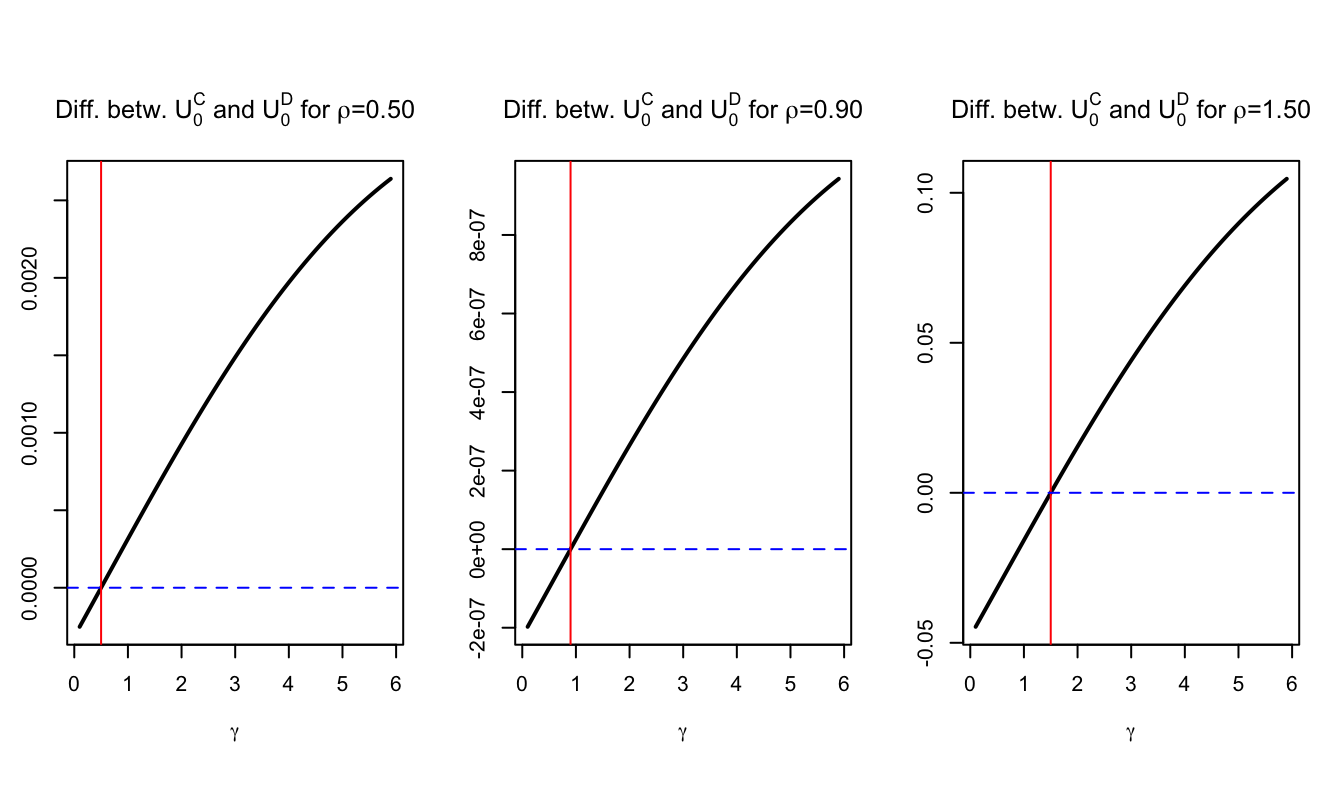
\includegraphics[width=0.95\linewidth]{TSM_files/figure-latex/EZresolution-1} \caption{Comparison of scenarios C and D illustrating the preference for early resolution of uncertainty.}\label{fig:EZresolution}
\end{figure}

\hypertarget{the-sdf-with-epstein-zin-preferences}{%
\subsection{The SDF with Epstein-Zin preferences}\label{the-sdf-with-epstein-zin-preferences}}

Consider an asset that provides the payoff \(x_{t+1}\) at date \(t+1\).
The equilibrium price \(\pi_t(x_{t+1})\) of this asset is such that agents are indifferent between buying or not an additional unit \(\varepsilon\) of this asset.
That is, \(U_t = F(C_t,R_t(U_{t+1}))\) is also equal to:
\begin{eqnarray}
&&  F(C_t,R_t(\color{blue}{U_{t+1}})) \nonumber \\
&=&F(C_t-\varepsilon \pi_t(x_{t+1}),R_t(\color{blue}{F(C_{t+1}+\varepsilon x_{t+1},R_{t+1}(U_{t+2}))})).\label{eq:SDFV}
\end{eqnarray}
Appendix \ref{SDFEZ} shows that this implies that:
\[
\pi_t(x_{t+1}) = \mathbb{E}_t \left( x_{t+1} \mathcal{M}_{t,t+1} \right),
\]
where \(\mathcal{M}_{t,t+1}\), the SDF, is given by:
\begin{equation}
\mathcal{M}_{t,t+1}= \delta \left(\frac{C_{t+1}}{C_t}\right)^{-\rho}  \left(\frac{U_{t+1}}{R_{t}(U_{t+1})}\right)^{\rho-\gamma}.\label{eq:SSS}
\end{equation}

Recall that, for all asset \(i\) (whose return is \(R_{i,t}\)), we have (Eq. \eqref{eq:MRCov}):
\[
\mathbb{E}_t(R_{i,t+1} - R_{f,t}) = - (1 + R_{f,t}) \mathbb{C}ov_t(\mathcal{M}_{t,t+1},R_{i,t+1}).
\]
Hence, with Eq. \eqref{eq:SSS}, expected returns depend not only on covariances between returns and consumption growth (as in the C-CAPM) but also on covariances between returns and the next period utility index, which captures news about the investor's future prospects.
To make the formula operational, one has to find a proxy for the utility. One can show that this utility is proportional to the value of the ``wealth portfolio''.

Before looking into it, Example \ref{exm:EZpricingInfo} explores an important implication of \eqref{eq:eq:SSS}, namely the fact that, with Epstein-Zin preferences, changes in the information regarding future consumption path is priced (in the sense that it results in specific risk premiums).

\begin{example}[Pricing information on future consumption path]
\protect\hypertarget{exm:EZpricingInfo}{}\label{exm:EZpricingInfo}

Consider the case where \(\rho = 1\) and log-normal conditionally homoskedastic consumption \citep{Cochrane_2005}. Using \(v_t = \log(U_t)\), we have:
\[
v_t = (1 - \delta) c_t + \delta \frac{1}{1 - \gamma} \log \mathbb{E}_t \left(\exp((1-\gamma)v_{t+1})\right).
\]
If \(c_t\) is log-normal, one can show that \(v_t\) is log-normal as well. Hence:
\begin{eqnarray}
v_t &=& (1 - \delta) c_t + \delta \mathbb{E}_t(v_{t+1}) + \frac{1}{2}\delta (1-\gamma) \sigma^2(v_{t+1})\nonumber \\
&=& (1 - \delta) \left( \sum_{j=0}^{\infty}  \delta^j \mathbb{E}_t (c_{t+j}) \right) + \frac{1}{2}\delta \frac{1-\gamma}{1-\delta} \sigma^2(v_{t+1}) (\#eq:v_rho1).
\end{eqnarray}
Besides, Eq. \eqref{eq:SSS} gives:
\begin{eqnarray*}
m_{t,t+1} &=& \log(\delta) - \rho \Delta c_{t+1} + (\rho - \gamma) \left(v_{t+1} - \frac{1}{1 - \gamma} \log \mathbb{E}_t \left(\exp((1-\gamma)v_{t+1})\right)\right)\\
&=& \log(\delta) - \rho \Delta c_{t+1} + (\rho - \gamma) \left(v_{t+1} - \mathbb{E}_t(v_{t+1}) - \frac{1}{2} \frac{1-\gamma}{1-\delta} \sigma^2(v_{t+1})\right).
\end{eqnarray*}
Using the \emph{expectation updating'' operator} \(\mathbb{E}_{t+1} - \mathbb{E}_t\), we obtain:
\[
(\mathbb{E}_{t+1} - \mathbb{E}_t) m_{t,t+1} = - \rho(\mathbb{E}_{t+1} - \mathbb{E}_t) c_{t+1} + (\rho - \gamma) (\mathbb{E}_{t+1} - \mathbb{E}_t) v_{t+1},
\]
which gives, when \(\rho = 1\) (using Eq. @ref(eq:v\_rho1)):
\begin{eqnarray}
(\mathbb{E}_{t+1} - \mathbb{E}_t) m_{t,t+1} &=& - (\mathbb{E}_{t+1} - \mathbb{E}_t) c_{t+1} +  \\
&& (1 - \gamma)(1 - \delta) (\mathbb{E}_{t+1} - \mathbb{E}_t) \left(  \sum_{j=1}^{\infty}  \delta^j c_{t+j}  \right).\nonumber
\end{eqnarray}

The previous equation can be rewritten as:
\begin{eqnarray}
&& (\mathbb{E}_{t+1} - \mathbb{E}_t) m_{t,t+1} \nonumber \\
&=& - \gamma(\mathbb{E}_{t+1} - \mathbb{E}_t)\Delta c_{t+1} +  \label{eq:sdfAbc}\\
&&  (1 - \gamma) \times \underbrace{ (\mathbb{E}_{t+1} - \mathbb{E}_t) \left(  \sum_{j=1}^{\infty}  \delta^j \Delta c_{t+1+j}  \right).}_{\mbox{innovation in long-run consumption growth}}\nonumber
\end{eqnarray}
Hence, news about future consumption growth affect the current SDF (marginal rate of substitution). As a consequence, shocks that correlate with updates of future consumption growth are ``priced''. The date-\(t\) prices---and more precisely their risk premium components---depend on the covariances between their payoffs and consumption on date \(t+1\), as well as future consumption growth (regarding \(t+h\), \(h>1\)).

\begin{quote}
If consumption is a random walk, then EZ preferences are observationally equivalent to power utility \citep{Kocherlakota_1990}.
\end{quote}

Consider the case where \(C_0 = C_1 = 1\).
At date \(t=1\), one get information about future consumption levels:

\begin{itemize}
\tightlist
\item
  {[}Case I{]} With probability 0.50, one will have \(C_t=\exp(\omega)\) for \(t\ge2\)
\item
  {[}Case II{]} With probability 0.50, one will have \(C_t=\exp(-\omega)\) for \(t\ge2\)
\end{itemize}

where \(\omega \ge 0\).
Eq. \eqref{eq:sdfAbc} implies that:
\[
m_{0,1} = \mathbb{E}_0(m_{0,1}) + (1 - \gamma)\delta \Delta c_{2}.
\]
(using that \(\mathbb{E}_0(\Delta c_{2})=0\) and that \(\mathbb{E}_1(\Delta c_{2})=\Delta c_{2}\).)
Assume that \(\mathbb{E}_0(m_{0,1})\) is such that \(\mathbb{E}_0(\mathcal{M}_{0,1})=\mathbb{E}_0(\exp(m_{0,1}))=1\) (i.e.~the risk-free rate is 0).
We consider the price of an asset that provides 1 at date 1 under Case II and 0 under Case I.
The price of this asset is:
\[
\mathbb{E}_t(\mathcal{M}_{t,t+1}\mathbb{I}_{\{Case II\}}) = \frac{1}{2} \times e^{\mathbb{E}_0(m_{0,1}) - (1 - \gamma)\delta \omega} \times 1.
\]

Figure \ref{fig:EZresolution2} shows the price of this asset for different values of \(\gamma\) and \(\omega\) (\(\delta=0.9\)). With expected utility time-separable preferences {[}Def. \ref{def:EUTSpref}{]} the price of such an asset would be 0.50 (represented by the dashed blue line).

\begin{figure}
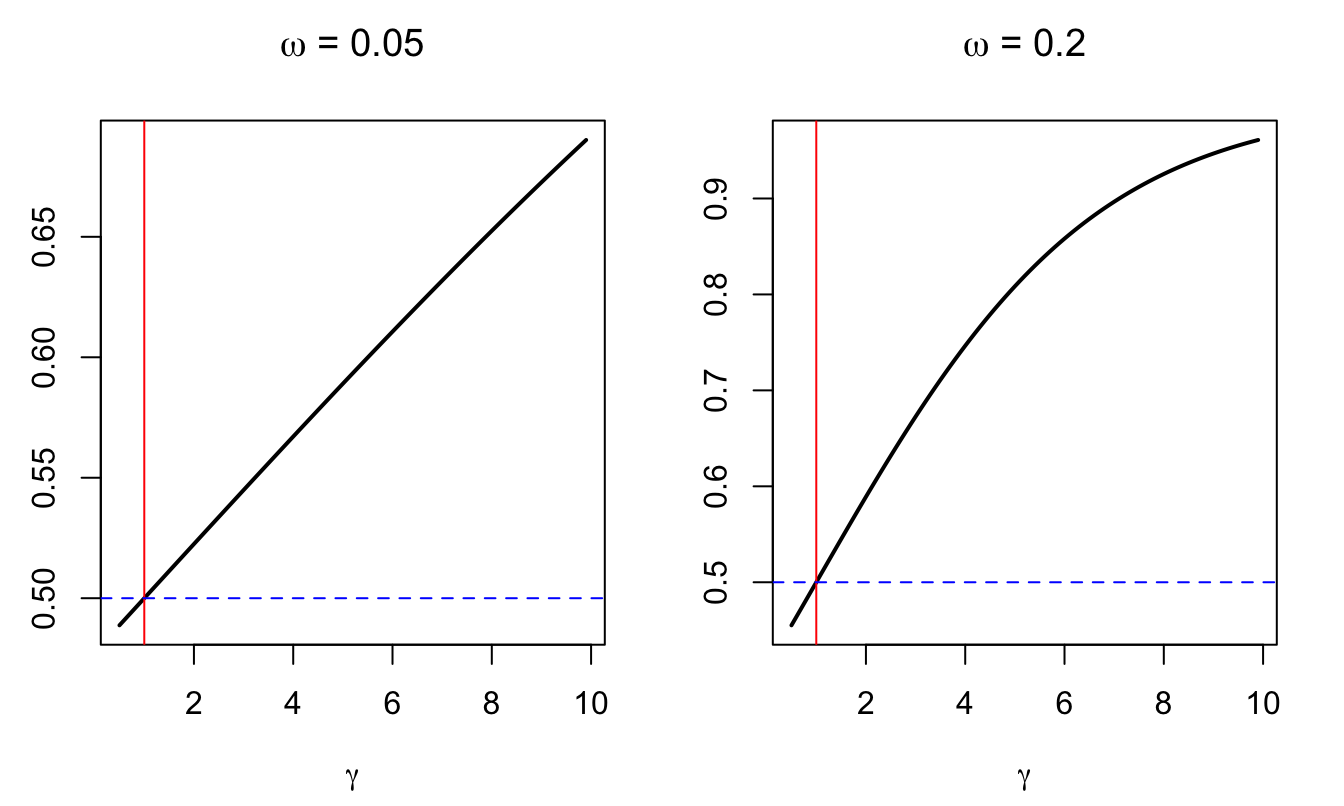
\includegraphics[width=0.95\linewidth]{TSM_files/figure-latex/EZresolution2-1} \caption{Price of an asset that pays 1 under Case II.}\label{fig:EZresolution2}
\end{figure}

\end{example}

Because \(F\) is homogenous of degree one in its arguments (\(C_t\) and \(R_t(U_{t+1})\)), the Euler's theorem yields \citep{HANSEN20073967}:
\begin{equation}
U_t = C_t \frac{\partial U_t}{\partial C_t} +  R_t(U_{t+1}) \frac{\partial U_t}{\partial R_t(U_{t+1})}.\label{eq:XXYXX}
\end{equation}
Taking the current consumption as numeraire, the wealth \(W_t\) is defined by:
\begin{equation}
W_t =   U_t \big/ \frac{\partial U_t}{\partial C_t}.\label{eq:WWWWW}
\end{equation}
It can be seen as a conversion of the intertemporal utility in terms of today's consumption. It can also be seen as a consumption-priced virtual asset that delivers aggregate consumption as its dividends on each time period; this asset is called \emph{wealth portfolio}.\footnote{Since \(F\) homogeneous of order 1, if all future consumption streams are multiplied by \(1+\epsilon\), then the utility becomes \((1+\epsilon)U_t\). Consider the asset that provides \(\epsilon C_{t+h}\) at all future periods (if one purchases \(\epsilon\) units of it). Expressed in consumption units, the equilibrium unit price of this asset (\(\mathcal{W}_t\), say) must satisfy \(-\epsilon U_t + \epsilon \mathcal{W}_t (\partial U_t / \partial C_t)=0\). According to Eq. \eqref{eq:WWWWW}, we have \(\mathcal{W}_t = W_t\).}

Using that \(\frac{\partial U_t}{\partial C_t}=(1 - \delta)(V_t^\rho)/(C_t^{\rho})\), we get (using Eq. \eqref{eq:WWWWW}):
\begin{equation}
W_t = \frac{U_t^{1-\rho}C_t^\rho}{1 - \delta}.\label{eq:WWW}
\end{equation}
Let's denote by \(R_{a,t+1}\) the return on the wealth portfolio. We have:
\begin{equation}
1+R_{a,t+1} := \frac{W_{t+1}}{W_t - C_t} = \frac{P_{a,t+1}+C_{t+1}}{P_{a,t}},\label{eq:Ra}
\end{equation}
where \(P_{a,t} := W_t - C_t\).

Using Eqs. \eqref{eq:EZpreferences2} and \eqref{eq:WWW}, it can be shown that:
\[
1+R_{a,t+1} = \left[ \delta \left( \frac{C_{t+1}}{C_t} \right)^{-\rho} \left( \frac{R_t(U_{t+1})}{U_{t+1}} \right)^{1-\rho} \right]^{-1},
\]
which is equivalent to:
\[
\frac{U_{t+1}}{R_t(U_{t+1})} = \left[ \delta (1+ R_{a,t+1}) \left( \frac{C_{t+1}}{C_t} \right)^{-\rho}  \right]^{\frac{1}{1-\rho}}.
\]
Substituting in Eq. \eqref{eq:SSS} gives:
\begin{equation}
\mathcal{M}_{t,t+1} =  \delta^{\theta} (1+R_{a,t+1})^{\theta - 1} \left( \frac{C_{t+1}}{C_t} \right)^{- \frac{\theta}{\psi}}
\end{equation}
where
\[
\theta = \frac{1-\gamma}{1-\rho} \quad and \quad \psi = \frac{1}{\rho}.
\]
Therefore (using \(\exp(r_{a,t+1}):=1+R_{a,t+1}\)):
\begin{equation}
\boxed{\log(\mathcal{M}_{t,t+1}) = \theta \log \delta - \frac{\theta}{\psi} \Delta \log(C_{t+1}) - (1-\theta) r_{a,t+1}.}\label{eq:sdfEZ}
\end{equation}

Let's take the log of Eq. \eqref{eq:Ra}:
\begin{eqnarray*}
r_{a,t+1} &=& \log(P_{a,t+1}+C_{t+1}) - \log(P_{a,t})\\
&=& z_{t+1} - z_t + g_{t+1} + \log(1 + C_{t+1} / P_{a,t+1}).
\end{eqnarray*}
where \(z_t = \log(P_{a,t}/C_t)\) is the log price-consumption ratio.
Let's denote by \(\bar{z}\) the unconditional mean of \(z_t\). If \(z_t - \bar{z}\) is small, we have:
\begin{eqnarray*}
\log[1 + C_{t+1} / P_{a,t+1}] &=& \log[1 + \exp(-z_{t+1})]\\
&\approx& \log[1 + \exp(-\bar{z})\{1 - (z_{t+1}- \bar{z})\}]\\
&\approx& \log[1 + \exp(-\bar{z}) - \exp(-\bar{z})(z_{t+1}- \bar{z})]\\
&\approx& \log[1 + \exp(-\bar{z})] - \frac{z_{t+1}- \bar{z}}{1 + \exp(\bar{z})}.
\end{eqnarray*}
Therefore:
\begin{equation}
\boxed{r_{a,t+1} \approx \kappa_0 + \kappa_1 z_{t+1} - z_t + g_{t+1},}\label{eq:approxRa}
\end{equation}
where \(\kappa_1= \dfrac{\exp(\bar{z})}{1 + \exp(\bar{z})}\) and \(\kappa_0 = \log(1 + \exp(\bar{z})) + \kappa_1 \bar{z}\).

\begin{quote}
The approximation underlying Eq. \eqref{eq:approxRa} is the same as that used by \citet{Campbell_Shiller_1988} used to linearize stock returns.
\end{quote}

For any asset \(i\), whose return is \(1+R_{i,t+1}\), we have:
\begin{equation}
1 = \mathbb{E}_t(\mathcal{M}_{t,t+1}(1+R_{i,t+1})). \quad \mbox{(Euler equation)}\label{eq:Euler}
\end{equation}
The wealth portfolio should also satisfy the Euler equation. That is, for \(1+R_{i,t+1} = 1+R_{a,t+1} = \exp(r_{a,t+1})\), we get:
\begin{equation}
1 = \mathbb{E}_t \left[ \exp\left(\theta \log \delta - \frac{\theta}{\psi} \Delta \log(C_{t+1}) + \theta r_{a,t+1} \right) \right].\label{eq:sdfRa}
\end{equation}

\begin{quote}
The previous equation can be used to determine approximately exponential affine SDF. (Indeed, \eqref{eq:sdfEZ} shows that the SDF is approximately exponential affine if \(\Delta \log(C_{t+1})\) and \(r_{a,t+1}\) are affine functions of the state vector.) \citet{Bansal_Yaron_2004} propose the follopwing approach: (a) Conjecture that the log price-consumption ratio \(z_t\) is linear in the sate vector, of the form \(A_0 + A_1'w_t\), say. (b) Then use the fact that the Euler equation has to hold for all values of the state variables to solve for \(A_0\) and \(A_1\).
\end{quote}

\begin{quote}
The same methodology can apply to any asset \(i\). For instance, consider a stock paying dividends \(D_{i,t}\) on each period. The \citet{Campbell_Shiller_1988} approximation implies that \(r_{i,t+1} \approx \kappa_0 + \kappa_1 z_{i,t+1} - z_{i,t} + d_{i,t+1}\) where \(d_{i,t+1}\) is the log-growth rate of dividends and where \(z_{i,t} = \log(P_{i,t}/D_t)\) is the log price-dividend ratio. If \(d_{i,t+1}\) is affine in the state vector, one can then posit that it is also the case of \(z_t= A_{i,0}+A_{i,1}'w_t\), and use the Euler equation
\begin{equation}
1 = \mathbb{E}_t \left[ \exp\left(\theta \log \delta - \frac{\theta}{\psi} \Delta \log(C_{t+1}) - (1 - \theta) r_{a,t+1} + r_{i,t+1} \right) \right].\label{eq:sdfRi}
\end{equation}
to solve for \(A_{i,0}\) and \(A_{i,1}\).
\end{quote}

\hypertarget{long-run-risk-model}{%
\subsection{Long-run risk model}\label{long-run-risk-model}}

We have shown that the CCAPM had difficulties in generating large average excess returns without implying unreasonable risk aversion parameters.
As will be shown later (notably in the \citet{Bansal_Yaron_2004}'s framework), E-Z preferences can address this problem.
With time-separable utilities, average excess returns (i.e.~risk premiums) had to be accounted by the sole correlation between stock returns and current consumption.
With E-Z preferences, another key correlation is that between stock returns and updates about future consumption growth {[}second term in Eq. \eqref{eq:sdfAbc}{]}.
For this second channel to be relevant, observed excess returns should positively correlate to the updates of expectations of long-term consumption. See Figure \ref{fig:SPF10yrStock}.

\begin{figure}
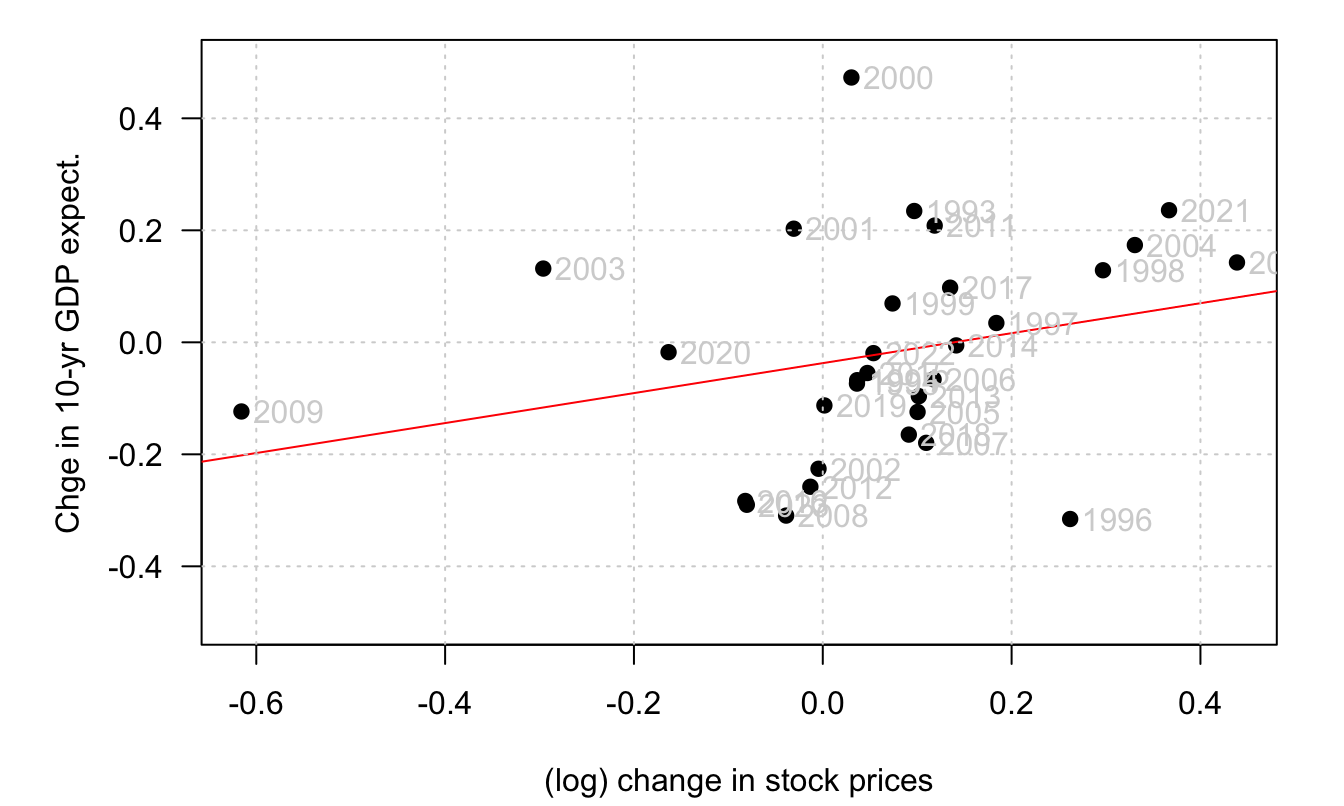
\includegraphics[width=0.95\linewidth]{TSM_files/figure-latex/SPF10yrStock-1} \caption{Sources: SPF Philadelphia and Wilshire 5000 Price Index (FRED database).}\label{fig:SPF10yrStock}
\end{figure}

\citet{Bansal_Yaron_2004} show that the combination of long-run risks and Epstein-Zin preferences allow to address several asset-pricing puzzles. A \href{https://jrenne.shinyapps.io/LRRModels}{web interface} present outputs of the approach. It also allows to simulate the model dynamics and to assess the influence of the parameterization.

In \citet{Bansal_Yaron_2004}'s model, consumption is affected by short-run (high-frequency) and long-run (low frequency) risks. They consider two versions of their model: an homoskedastic one and an heteroskedastic one. In the latter, the conditional variance of consumption moves over time.

\begin{example}[Bansal and Yaron (2004), homoskedastic]
\protect\hypertarget{exm:BYHomsk}{}\label{exm:BYHomsk}

\citet{Bansal_Yaron_2004} postulate the following dynamics for the economy:
\begin{eqnarray*}
x_{t+1} &=& \rho_x x_t + \phi_e \sigma e_{t+1}\\
\Delta c_{t+1} = g_{t+1} &=& \mu + x_t + \sigma \eta_{t+1}\\
g_{d,t+1} &=& \mu_d + \phi x_t + \phi_d \sigma u_{t+1},
\end{eqnarray*}
where \(e_{t+1},\eta_{t+1},u_{t+1} \sim i.i.d. \mathcal{N}(0,1)\). In this model,
\(\mu + x_t\) and \(\mu_d + \phi x_t\) are, respectively, the conditional expectations of consumption growth (\(g_t\)) and dividend growth (\(g_{d,t}\)). Processes \(g_t\) and \(g_{d,t}\) are exogenous. The model is solved by finding associated processes \(r_{a,t}\) and \(r_{m,t}\) that make the model internally consistent. These returns have to satisfy both Eqs. \eqref{eq:approxRa} and \eqref{eq:sdfRa}.
\(z_t\) and \(z_{m,t}\) are the log price-consumption and price-dividend ratios, respectively, i.e.:
\[
z_t = \log\left(\frac{P_{a,t}}{C_t}\right) \quad and \quad z_{m,t} = \log\left(\frac{P_{m,t}}{C_t}\right).
\]
The price of a claim on aggregate consumption is not observable (return: \(R_{a,t}\)), contrary to the price of the market portfolio (return: \(R_{m,t}\)).

The solution approach is as follows:

\begin{itemize}
\tightlist
\item
  Posit that \(z_t = A_0 + A_1 x_t\);
\item
  substitute the last expression into Eq. \eqref{eq:approxRa} and
\item
  inject \(r_{a,t+1}\) in Eq. \eqref{eq:sdfRa} and look for the values of \(A_0\) and \(A_1\) that satisfy this Euler equation.
\end{itemize}

Doing the same for \(z_{m,t}\) yields to:
\begin{equation}
A_1 = \frac{1- \dfrac{1}{\psi}}{1 - \kappa_1 \rho_x} \quad and \quad A_{1,m} = \frac{\Phi- \dfrac{1}{\psi}}{1 - \kappa_{1,m} \rho_x}.\label{eq:solABY1}
\end{equation}
If the IES \(\psi > 1\), then \(A_1 > 0\); the price-consumption ratio increases with long-term growth.

\begin{figure}

{\centering 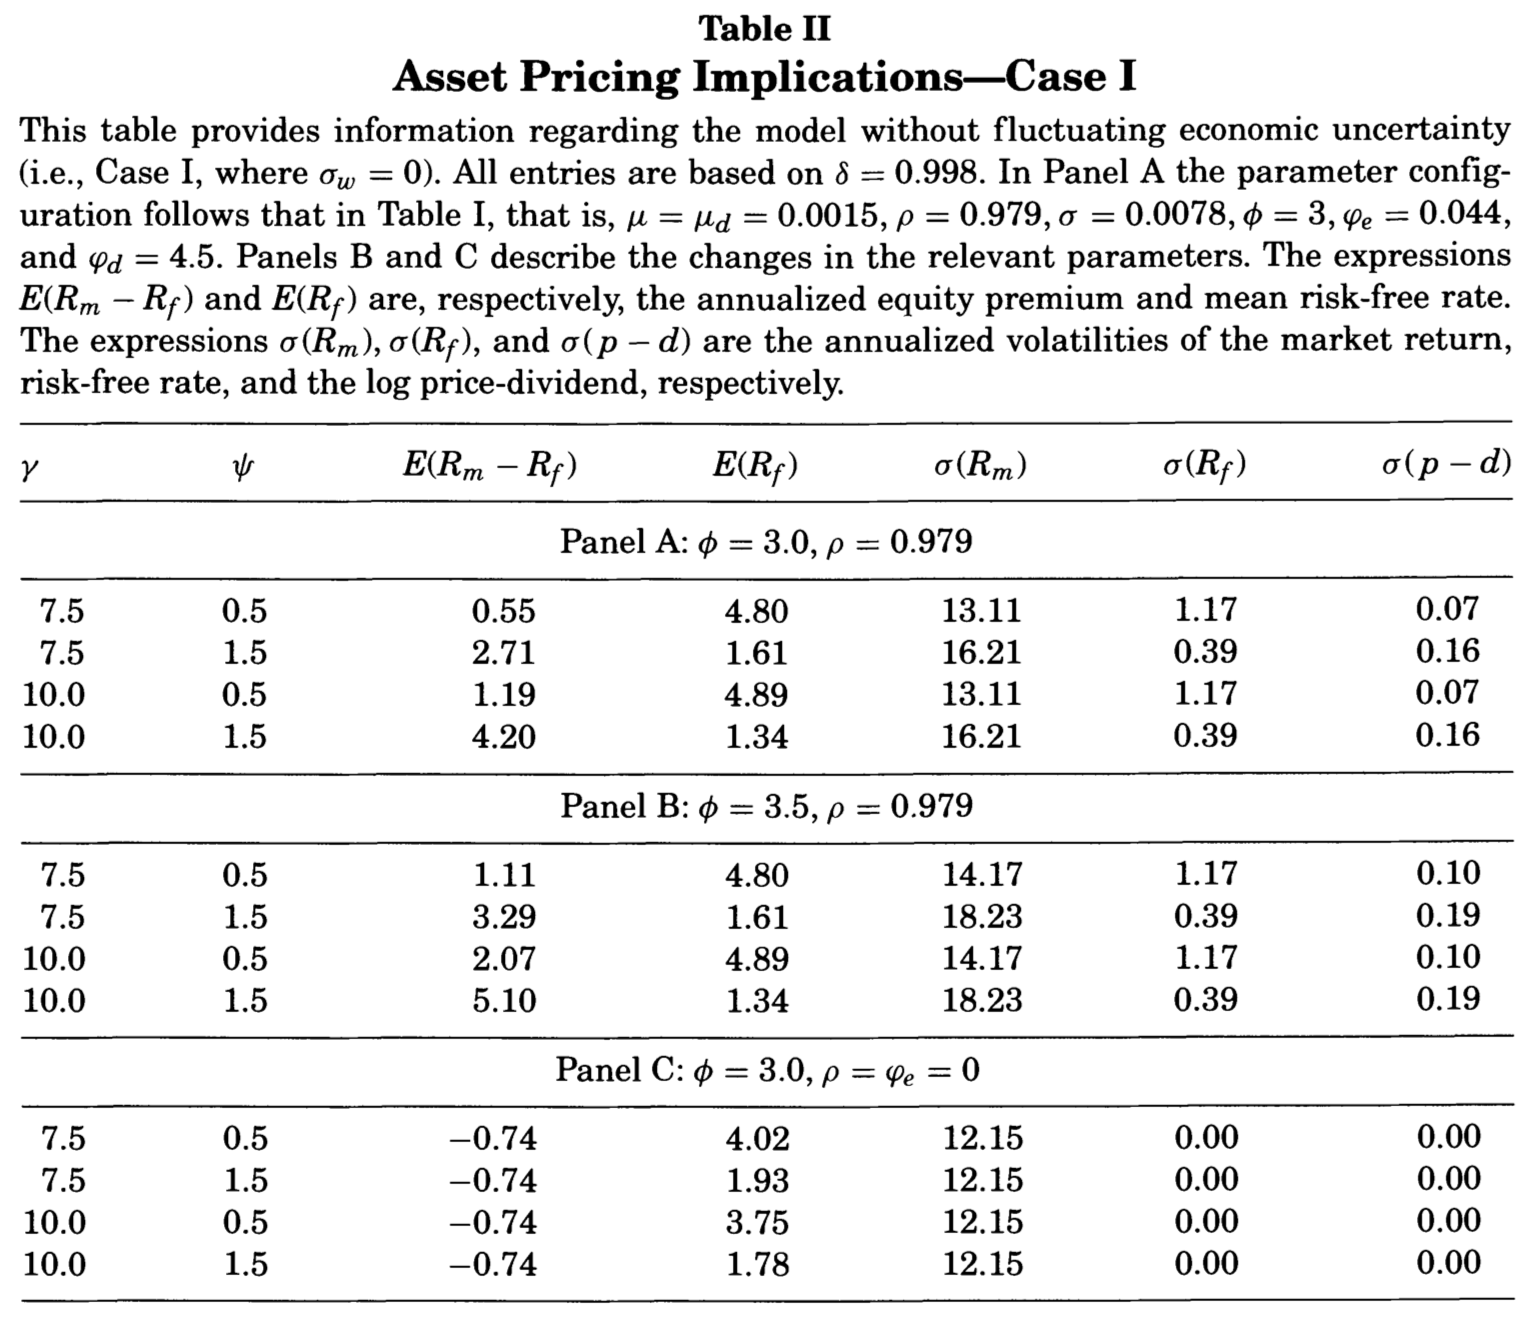
\includegraphics[width=1\linewidth]{figures/table_BY2} 

}

\caption{Source: Bansal and Yaron (2004).}\label{fig:BY2}
\end{figure}

\end{example}

\begin{quote}
\textbf{About the solution procedure}. Eq. \eqref{eq:solABY1} shows that the \(A_i\)s depends on the \(\kappa_i\)s. Eq. \eqref{eq:approxRa} shows that the \(\kappa_i\)s depend on \(\bar{z}\).
Hence, in particular, \(A_0 = f(\bar{z})\). But, in turn, since \(z_t = A_0 + A_1 x_t\), we have \(\bar{z}=A_0 + A_1 \bar{x}=A_0\). For the model to be internally consistent, we should have \(\bar{z}=f(\bar{z})\). Hence, there is a fixed-point problem (\(\bar{z}\) cannot be chosen arbitrarily).
\end{quote}

\begin{example}[Bansal and Yaron (2004), heteroskedastic]
\protect\hypertarget{exm:BYHeterosk}{}\label{exm:BYHeterosk}

\citet{Bansal_Yaron_2004} consider a second version of their model. They introduce a novel factor, \(\sigma_t\), that generates time-variation in the conditional variances of consumption and dividends:
\begin{eqnarray}
x_{t+1} &=& \rho_x x_t + \phi_e \sigma_t e_{t+1} \nonumber\\
g_{t+1} &=& \mu + x_t + \sigma_t \eta_{t+1} \nonumber\\
g_{d,t+1} &=& \mu_d + \phi x_t + \phi_d \sigma_t u_{t+1} \nonumber\\
\sigma_{t+1}^2 &=& \sigma^2 + \nu_1(\sigma^2_t -\sigma^2) + \sigma_w w_{t+1}, \label{eq:BYheteroscked}
\end{eqnarray}
where \(e_{t+1},\eta_{t+1},u_{t+1},w_{t+1} \sim i.i.d. \mathcal{N}(0,1)\).
Here, the posited solution for \(z_t\) is:
\[
z_t = A_0 + A_1 x_t + {\color{red}A_2 \sigma^2_t}.
\]
\(A_1\) is unchanged. \(A_2\) is given by (similar form for \(A_{2,m}\)):
\[
A_2 = \frac{0.5 \left[ \left(\theta - \dfrac{\theta}{\psi}\right)^2 + (\theta A_1 \kappa_1 \phi_e)^2 \right]}{\theta(1 - \kappa_1 \nu_1)}.
\]

\begin{figure}

{\centering 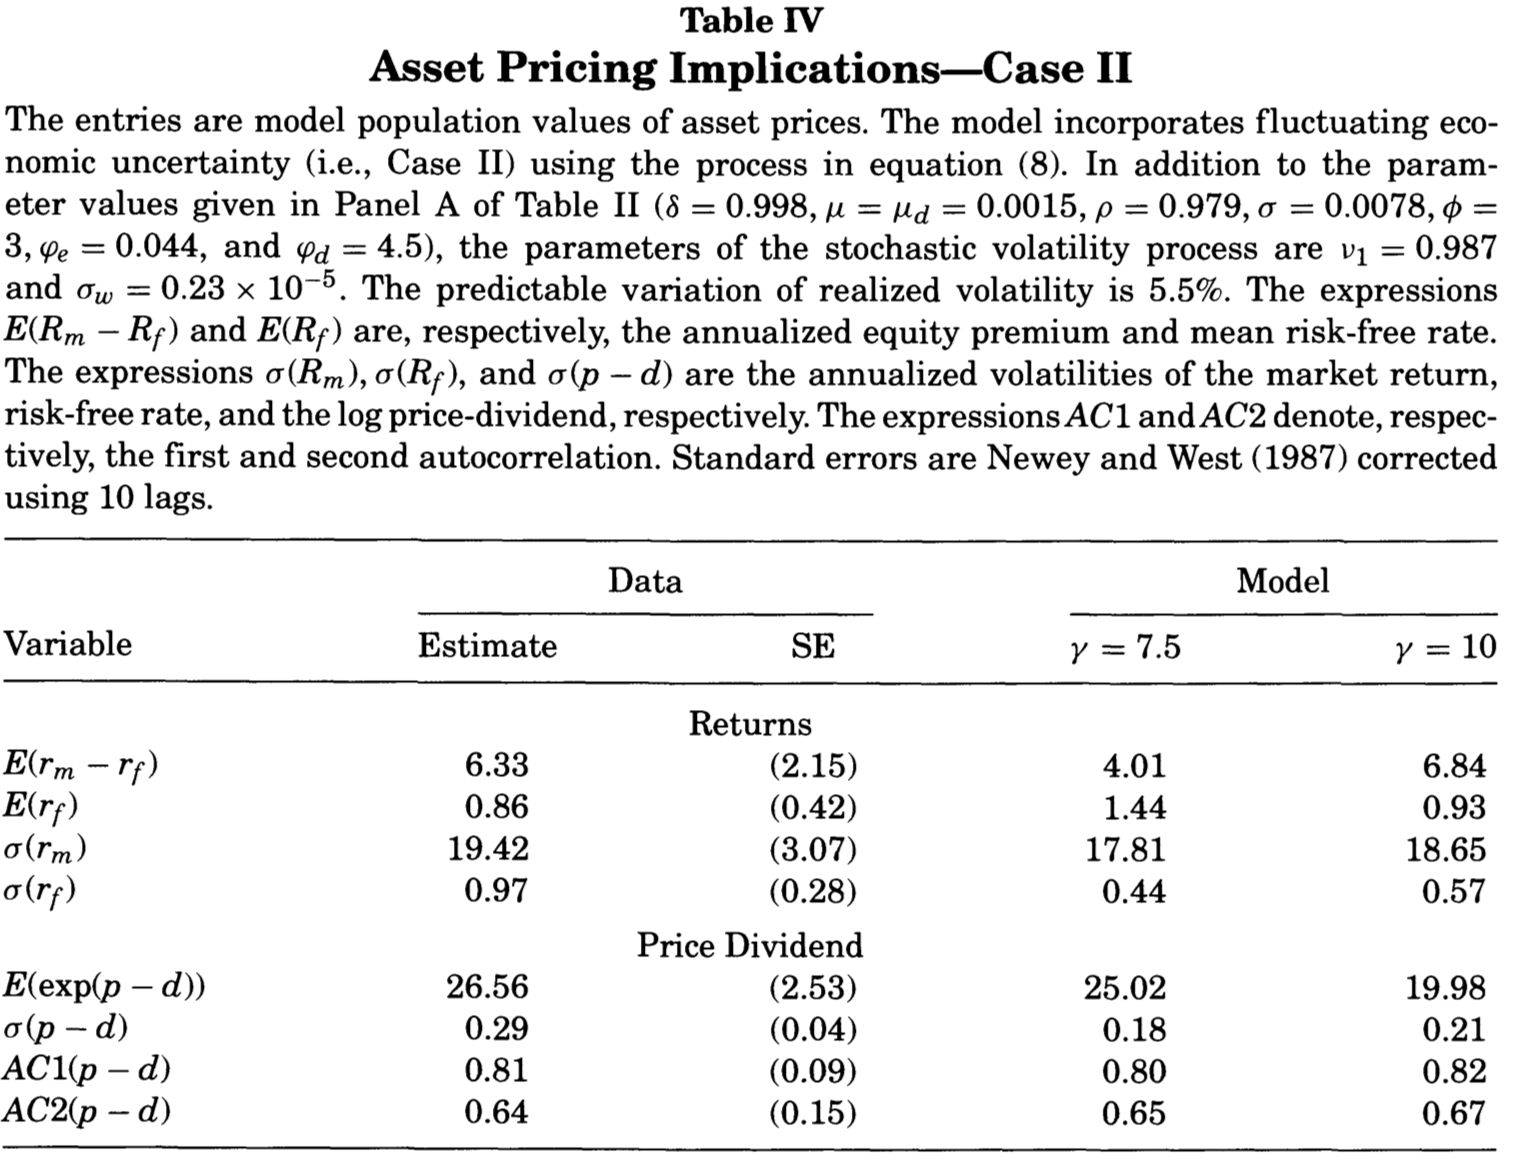
\includegraphics[width=1\linewidth]{figures/table_BY4} 

}

\caption{Source: Bansal and Yaron (2004).}\label{fig:BY4}
\end{figure}

\end{example}

\hypertarget{preferred-habitat-model-of-the-term-structure-of-interest-rate}{%
\section{Preferred-habitat model of the term-structure of interest rate}\label{preferred-habitat-model-of-the-term-structure-of-interest-rate}}

A very different type of asset-pricing structural model has been introduced by \citet{Greenwood_Vayanos_2014} and \citet{Vayanos_Vila_2021}. In the present section, we derive the approximate yield curve solution to this type of model in discrete-time (while the original model is written in continuous time); this derivations is broadly based on \citet{Hamilton_Wu_2012} and \citet{Hayashi_2018}.

Term structure models based on preferred habitat theory are a class of financial models that extend traditional yield curve models by incorporating the notion that some investors or issuers exhibit preferences for specific maturity segments, or ``habitats,'' in the bond market. These models provide a nuanced understanding of how market participants' varying preferences for maturity segments influence interest rates and the overall shape of the yield curve.

In these models, there are two broad categories of market participants: the preferred-habitant investors/issuers and the arbitrageurs. The latter have no preferred habitat, they aim to maximize their wealth under risk constraints.

Denote by \(P_{n,t}\) the date-\(t\) prices of a \(n\)-period conventional zero-coupon bonds, and by \(N\) the maximum bond maturity. Arbitrageurs' wealth evolves according to:
\[
W_{t+1} = \left(\sum_{n=1}^N z_{n,t}\frac{P_{n-1,t+1}}{P_{n,t}}\right)W_t,
\]
where \(z_{n,t}\) is the fraction of wealth invested in \(n\)-period bonds on date \(t\). The portfolio's return between dates \(t\) and \(t+1\) is:
\begin{eqnarray*}
r_{t,t+1} &=& \frac{W_{t+1}-W_t}{W_t}=
\sum_{n=1}^N z_{n,t}\left(\frac{P_{n-1,t+1}}{P_{n,t}}-1\right) = \sum_{n=1}^N z_{n,t}r_{n,t,t+1},
\end{eqnarray*}
where \(r_{n,t,t+1}\) is the one-period return of the \(n\)-period bond.

\begin{hypothesis}
\protect\hypertarget{hyp:prefArbit}{}\label{hyp:prefArbit}On date \(t\), arbitrageurs determine \(z_t=[z_{1,t},\dots,z_{N,t}]'\) so as to maximize:
\[
\mathbb{E}_t(r_{t,t+1}) - \frac{\gamma}{2}\mathbb{V}ar_t(r_{t,t+1}),
\]
under the constraint that \(\sum_n^N z_{n,t} = 1\).
\end{hypothesis}

\begin{hypothesis}
\protect\hypertarget{hyp:dynF}{}\label{hyp:dynF}The state of the economy is characterized by a \(m\)-dimensional vector of factors, denoted \(f_t\), which follows a Gaussian vector auto-regressive process of order one:
\[
f_t = \mu_f + \Phi f_{t-1} + \Sigma \varepsilon_t,
\]
with \(\varepsilon_t \sim\,i.i.d.\,\mathcal{N}(0,Id)\).
\end{hypothesis}

Let us denote by \(y_{n,t}\) the yield-to-maturity of a \(n\)-period zero-coupon bond. We have:
\begin{equation}
y_{n,t} = - \frac{1}{n}\log P_{n,t}.\label{eq:Pandy}
\end{equation}

\begin{proposition}[Links between bond prices]
\protect\hypertarget{prp:prop111}{}\label{prp:prop111}Under Assumptions \ref{hyp:prefArbit} and \ref{hyp:dynF}, and if the prices of \(n\)-period zero-coupon bonds are given by exponential affine functions of \(f_t\), that is, if
\begin{equation}
P_{n,t} = \exp(a_{n,t} + b_{n,t}'f_t), \label{eq:PPs}    
\end{equation}
(which implies, in particular, that we must have \(y_{1,t} = - a_1 - b_1'f_t\)), then \(a_n\) and \(b_n\) approximately verify, for \(n \ge 2\):
\begin{eqnarray}
-a_1-b_1' f_t &\approx& a_{n-1} + b_{n-1}'\mu_f  - a_{n} + b_{n-1}'\Phi f_t - b_{n}'f_{t} + \nonumber \\ &&\frac{1}{2}b_{n-1}'\Sigma \Sigma'b_{n-1} - \gamma b_{n-1}'\Sigma\Sigma'\Theta' z_t, \label{eq:Lagr1B}
\end{eqnarray}
where \(\Theta\) is an \(N \times m\) matrices whose \(n^{th}\) rows is \(b_{n-1}'\). (Note that the first rows of this matrix is filled with zeros.)
\end{proposition}

\begin{proof}
Using that \(z_{1,t} = 1 - \sum_{n=2}^{N}z_{n,t}\), and noting that \(y_{1,t}=r_{1,t,t+1}\), one obtains the following first-order conditions to the arbitrageurs' problem (as defined by Assumption \ref{hyp:prefArbit}), for \(n \ge 2\):
\begin{eqnarray}
y_{1,t} &=& \mathbb{E}_t(r_{n,t,t+1}) - \frac{\gamma}{2} \frac{\partial}{\partial z_{n,t}} \mathbb{V}ar_t(r_{t,t+1}). \label{eq:Lagr1}
\end{eqnarray}
When bond prices are as in \eqref{eq:PPs}, we have:
\begin{eqnarray*}
r_{n,t,t+1} &=& P_{n-1,t+1}/P_{n,t}-1 = \exp(a_{n-1} + b_{n-1}'f_{t+1} - a_{n} - b_{n}'f_{t})-1,
\end{eqnarray*}
from which we get the following approximations, assuming that one-period bond returns are small \citep{Hamilton_Wu_2012}:
\begin{eqnarray}
\mathbb{E}_t(r_{n,t,t+1}) &\approx&  a_{n-1} + b_{n-1}'\mu_f  - a_{n} + b_{n-1}'\Phi f_t - b_{n}'f_{t}\nonumber\\
&&+ \frac{1}{2}b_{n-1}'\Sigma \Sigma'b_{n-1} \label{eq:Exp1}
\end{eqnarray}
Moreover, using \(r_{n,t,t+1} \approx \log(P_{n-1,t+1}/P_{n,t})\), we get:
\begin{equation}
\mathbb{V}ar_t(r_{t,t+1}) \approx z_t'\Theta\Sigma\Sigma'\Theta' z_t.\label{eq:Var}
\end{equation}
Eq. \eqref{eq:Var} implies in particular that:
\begin{eqnarray*}
\frac{\partial}{\partial z_t} \mathbb{V}ar_t(r_{t,t+1}) &\approx& 2 \Theta\Sigma\Sigma'\Theta' z_t,
\end{eqnarray*}
which, in turn, gives:
\begin{eqnarray*}
\frac{\partial}{\partial z_{n,t}} \mathbb{V}ar_t(r_{t,t+1}) &\approx& 2 b_{n-1}'\Sigma\Sigma'\Theta' z_t.
\end{eqnarray*}
Using the previous equation as well as \eqref{eq:Exp1} in \eqref{eq:Lagr1} leads to \eqref{eq:Lagr1B}.
\end{proof}

\begin{hypothesis}[Bond supply]
\protect\hypertarget{hyp:supply}{}\label{hyp:supply}Bond supplies, expressed as fractions of the arbitrageurs' wealth, depend on a time-varying component (\(\alpha_n + \beta_n' f_t\)) and on yields-to-maturity. Specifically:
\begin{eqnarray}
s_{n,t} &=& (\alpha_n + {\beta_n}' f_t) - \zeta_n y_{n,t}. \label{eq:supply1}
\end{eqnarray}
\end{hypothesis}

\begin{definition}[Equilibrium]
\protect\hypertarget{def:Equilib}{}\label{def:Equilib}In equilibrium, bond market clears (for each maturity). Arbitrageurs maximize the problem defined in Assumption \ref{hyp:prefArbit}, which determines the bond demand, and bond supply is determined by Assumption \ref{hyp:supply}.
\end{definition}

\begin{proposition}[Bond prices]
\protect\hypertarget{prp:PropII}{}\label{prp:PropII}Under Assumptions \ref{hyp:prefArbit} to \ref{hyp:supply}, and if bond prices are exponential affine in \(f_t\), then the loadings \(a_n\) and \(b_n\)---which appear in equation \eqref{eq:PPs}---approximately satisfy the following recursive equations, for \(n\ge 1\):
\begin{equation}
\left\{
\begin{array}{cll}
a_n &\approx& a_1 + a_{n-1} + b_{n-1}'\mu_f^{\mathbb{Q}} + \frac{1}{2}b_{n-1}'\Sigma \Sigma'b_{n-1} \\
b_n &\approx& b_1 + {\Phi^{\mathbb{Q}}}'b_{n-1},
\end{array}
\right.\label{eq:recursConventio}
\end{equation}
with \(a_0=0\), \(b_0=0\), and where
\begin{equation}
\mu_f^{\mathbb{Q}} = \mu_f - \Sigma \lambda \quad \mbox{and} \quad \Phi^{\mathbb{Q}} = \Phi - \Sigma \Lambda,\label{eq:muPHIQ}
\end{equation}
with
\begin{equation}
\lambda = \gamma \Sigma' \Theta'\mathcal{A} \quad \mbox{and} \quad \Lambda = \gamma \Sigma' \Theta'\mathcal{B},\label{eq:lambdas} 
\end{equation}
\(\mathcal{A}\) being a \(N\)-dimensional vector whose \(n^{th}\) entry is \(\alpha_n + \frac{1}{n}\zeta_n a_n\), and \(\mathcal{B}\) being a \(N \times m\) matrix whose \(n^{th}\) row is \((\beta_n + \frac{1}{n}\zeta_n b_n)'\). (Matrix \(\Theta\) is defined in Proposition \ref{prp:prop111}.)
\end{proposition}

\begin{proof}
If prices are as in \eqref{eq:PPs}, and using \eqref{eq:Pandy}, we have:
\[
y_{n,t} = -\frac{1}{n}(a_n + b_n'f_t).
\]

Combining the last equation with \eqref{eq:supply1} gives:
\begin{eqnarray}
s_{n,t} &=& \alpha_n  + \frac{1}{n}\zeta_n a_n + \left(\beta_n + \frac{1}{n}\zeta_n b_n\right)'f_t.
\end{eqnarray}
At equilibrium, we have \(z_{n,t}=s_{n,t}\), which imples that the \(z_t\)'s are affine functions of \(f_t\). Specifically, we have:
\[
z_t = \mathcal{A} + \mathcal{B}f_t.
\]
This implies that we have:
\[
\gamma \Sigma' B'z_t  = \lambda + \Lambda f_t,
\]
with \(\lambda\) and \(\Lambda\) given in \eqref{eq:lambdas}. Using these notations, \eqref{eq:Lagr1B} rewrites:
\begin{eqnarray*}
y_{1,t} &\approx& a_{n-1} + b_{n-1}'\mu_f  - a_{n} + b_{n-1}'\Phi f_t - b_{n}'f_{t} + \frac{1}{2}b_{n-1}'\Sigma \Sigma'b_{n-1} - b_{n-1}'\Sigma (\lambda + \Lambda f_t).
\end{eqnarray*}
Using the notations introduced in \eqref{eq:muPHIQ}, this leads to:
\begin{eqnarray}
&&- a_1 - b_1' f_t \nonumber\\
&\approx& a_{n-1} + b_{n-1}'\mu_f^{\mathbb{Q}}  - a_{n} + b_{n-1}'\Phi^{\mathbb{Q}} f_t - b_{n}'f_{t} + \frac{1}{2}b_{n-1}'\Sigma \Sigma'b_{n-1}. \label{eq:Lagr1C}
\end{eqnarray}
The recursions \eqref{eq:recursConventio} are required for \eqref{eq:Lagr1C} to be satisfied for any value of \(f_t\).
\end{proof}

\begin{quote}
The first row of \(\Theta\) is \(b_0'=0\). As a result, looking at \eqref{eq:lambdas}, it appears that the first component entry of \(\mathcal{A}\) (namely \(\alpha_1 + \zeta_1 a_1\)) and the first row of \(\mathcal{B}\) (namely \(\beta_1' + \zeta_1 b_1'\)) do not appear in \(\lambda\), nor in \(\Lambda\). This gives the impression that the bond supply specification for one-period bond has no pricing impact. This is however false, as we must have:
\[
\sum_{n=1}^N z_{i,t} = 1.
\]
For this to hold for any value of \(f_t\), we need to have:
\begin{eqnarray}
\alpha_1 + \zeta_1 a_1 &=& 1 - \sum_{n=2}^N\mathcal{A}_i \label{eq:constr1}\\
\beta_1 + \zeta_1 b_1&=&  - \sum_{n=2}^N\mathcal{B}_i,\label{eq:constr2}
\end{eqnarray}
where \(\mathcal{B}_i\) is the \(i^{th}\) row of \(\mathcal{B}\). These two equations show that \(a_1\) and \(b_1\) cannot be chosen independently from the specification of the supply for one-period bonds (characterized by \(\alpha_1\), \(\beta_1\), and \(\zeta_1\)).
In particular, consider the case where one factor corresponds to the conventional short-term yield (a situation that is standard in the literature). Assume for instance that the first component of \(f_t\) is the conventional one-period yield. In that case, we have:
\[
a_1 = 0 \quad \mbox{and}\quad b_1 = [-1,0,0,\dots]'.
\]
Assume that \eqref{eq:supply1} holds for \(n \ge 2\). Proposition \ref{prp:PropII} then states that one can solve for the \((a_n,b_n)\)'s. However, it should then by checked that \(\alpha_1\), \(\beta_1\), and \(\zeta_1\) satisfy \eqref{eq:constr1} and \eqref{eq:constr2}. Alternatively, assuming for instance that \(\zeta_1\) is fixed, one can then deduce \(\alpha_1\) and \(\beta_1\).
\end{quote}

The following lines of codes build a discrete-time version of the model proposed by \citet{Vayanos_Vila_2021}. This model features two factors. The first (\(f_{1,t}\)) is the short-term interest rate, the seconf (\(f_{2,t}\)) is a supply factor. Parameters \(\zeta_n\), \(\alpha_n\), and \(\beta_{n,2}\), defining the specification of bond supplies (see Assumption \ref{hyp:supply}, are given by:\footnote{We have \(\beta_{n,1}=0\). That is, the short-term rate has no direct influence on the \(s_{n,t}\)'s.}
\begin{eqnarray}
\zeta_n &=& \zeta_0 n \exp(-\delta_\zeta n) \\
\beta_{n,2} &=& \kappa_{\beta} \big( \exp(-\delta_\zeta n) - \exp(-\delta_{\beta} n) \big) \\
\alpha_n &=& \kappa_\alpha \big( \exp(-\delta_\zeta n) - \exp(-\delta_{\beta,1} n) \big) \end{eqnarray}

Figure \ref{fig:VV1} shows the influence of the latter on bond supply (the \(s_{n,t}\)'s). Note that the figure shows only the \(\beta_{n,2}\)'s for \(n \ge 2\), since \(\beta_{1,2}\) is residual of the model solution.

\begin{Shaded}
\begin{Highlighting}[]
\FunctionTok{library}\NormalTok{(TSModels)}
\NormalTok{m }\OtherTok{\textless{}{-}} \DecValTok{2} \CommentTok{\# number of factors}
\NormalTok{N }\OtherTok{\textless{}{-}} \DecValTok{30} \CommentTok{\# maximum maturity}
\CommentTok{\# Calibration: see Table 1 in Vayanos{-}Vila:}
\NormalTok{kappa\_r     }\OtherTok{\textless{}{-}}\NormalTok{ .}\DecValTok{125}
\NormalTok{sigma\_r     }\OtherTok{\textless{}{-}}\NormalTok{ .}\DecValTok{0146}
\NormalTok{kappa\_beta  }\OtherTok{\textless{}{-}}\NormalTok{ .}\DecValTok{053}
\NormalTok{a.theta     }\OtherTok{\textless{}{-}} \DecValTok{3155}
\NormalTok{a.alpha     }\OtherTok{\textless{}{-}} \FloatTok{35.3}
\NormalTok{delta\_alpha }\OtherTok{\textless{}{-}}\NormalTok{ .}\DecValTok{297}
\NormalTok{delta\_theta }\OtherTok{\textless{}{-}}\NormalTok{ .}\DecValTok{307}
\NormalTok{alpha       }\OtherTok{\textless{}{-}} \FloatTok{5.21}
\NormalTok{r\_bar       }\OtherTok{\textless{}{-}} \FloatTok{4.8}
\NormalTok{a.theta0    }\OtherTok{\textless{}{-}} \DecValTok{289}
\CommentTok{\# Specif of minus short{-}rate:}
\NormalTok{a1 }\OtherTok{\textless{}{-}} \SpecialCharTok{{-}}\NormalTok{ r\_bar}\SpecialCharTok{/}\DecValTok{100} \CommentTok{\# minus mean of short{-}term rate}
\NormalTok{b1 }\OtherTok{\textless{}{-}} \FunctionTok{matrix}\NormalTok{(}\FunctionTok{c}\NormalTok{(}\SpecialCharTok{{-}}\DecValTok{1}\NormalTok{,}\FunctionTok{rep}\NormalTok{(}\DecValTok{0}\NormalTok{,m}\DecValTok{{-}1}\NormalTok{)),}\AttributeTok{ncol=}\DecValTok{1}\NormalTok{) }\CommentTok{\# The first factor is r\_t}
\CommentTok{\# Specify factors\textquotesingle{} dynamics:}
\NormalTok{mu\_f  }\OtherTok{\textless{}{-}} \FunctionTok{matrix}\NormalTok{(}\DecValTok{0}\NormalTok{,m,}\DecValTok{1}\NormalTok{)}
\NormalTok{Phi   }\OtherTok{\textless{}{-}} \FunctionTok{diag}\NormalTok{(}\FunctionTok{c}\NormalTok{(}\DecValTok{1}\SpecialCharTok{{-}}\NormalTok{kappa\_r,}\DecValTok{1}\SpecialCharTok{{-}}\NormalTok{kappa\_beta))}
\NormalTok{Sigma }\OtherTok{\textless{}{-}} \FunctionTok{diag}\NormalTok{(}\FunctionTok{c}\NormalTok{(sigma\_r,sigma\_r))}
\CommentTok{\# Specify supply of bonds:}
\NormalTok{a }\OtherTok{\textless{}{-}}\NormalTok{ a.alpha}\SpecialCharTok{/}\NormalTok{alpha;theta }\OtherTok{\textless{}{-}}\NormalTok{ a.theta}\SpecialCharTok{/}\NormalTok{a; theta0 }\OtherTok{\textless{}{-}}\NormalTok{ a.theta0}\SpecialCharTok{/}\NormalTok{a}
\NormalTok{Alpha      }\OtherTok{\textless{}{-}} \FunctionTok{matrix}\NormalTok{(theta0 }\SpecialCharTok{*}\NormalTok{ (}\FunctionTok{exp}\NormalTok{(}\SpecialCharTok{{-}}\NormalTok{delta\_alpha}\SpecialCharTok{*}\NormalTok{(}\DecValTok{1}\SpecialCharTok{:}\NormalTok{N)) }\SpecialCharTok{{-}}
                                 \FunctionTok{exp}\NormalTok{(}\SpecialCharTok{{-}}\NormalTok{delta\_theta}\SpecialCharTok{*}\NormalTok{(}\DecValTok{1}\SpecialCharTok{:}\NormalTok{N))),N,}\DecValTok{1}\NormalTok{)}
\NormalTok{Beta      }\OtherTok{\textless{}{-}} \FunctionTok{matrix}\NormalTok{(}\DecValTok{0}\NormalTok{,N,m)}
\NormalTok{Beta[,}\DecValTok{2}\NormalTok{]  }\OtherTok{\textless{}{-}}\NormalTok{ theta }\SpecialCharTok{*}\NormalTok{ (}\FunctionTok{exp}\NormalTok{(}\SpecialCharTok{{-}}\NormalTok{delta\_alpha}\SpecialCharTok{*}\NormalTok{(}\DecValTok{1}\SpecialCharTok{:}\NormalTok{N)) }\SpecialCharTok{{-}}
                        \FunctionTok{exp}\NormalTok{(}\SpecialCharTok{{-}}\NormalTok{delta\_theta}\SpecialCharTok{*}\NormalTok{(}\DecValTok{1}\SpecialCharTok{:}\NormalTok{N)))}
\NormalTok{Zeta      }\OtherTok{\textless{}{-}}\NormalTok{ alpha }\SpecialCharTok{*} \FunctionTok{matrix}\NormalTok{(}\DecValTok{1}\SpecialCharTok{:}\NormalTok{N }\SpecialCharTok{*} \FunctionTok{exp}\NormalTok{(}\SpecialCharTok{{-}}\NormalTok{delta\_alpha}\SpecialCharTok{*}\NormalTok{(}\DecValTok{1}\SpecialCharTok{:}\NormalTok{N)),N,}\DecValTok{1}\NormalTok{)}

\NormalTok{model }\OtherTok{\textless{}{-}} \FunctionTok{list}\NormalTok{(}\AttributeTok{gamma =}\NormalTok{ a,}\AttributeTok{mu\_f =}\NormalTok{ mu\_f,}\AttributeTok{Phi =}\NormalTok{ Phi,}\AttributeTok{Sigma =}\NormalTok{ Sigma,}
              \AttributeTok{Alpha =}\NormalTok{ Alpha,}\AttributeTok{Beta =}\NormalTok{ Beta,}\AttributeTok{Zeta =}\NormalTok{ Zeta,}\AttributeTok{a1 =}\NormalTok{ a1,}\AttributeTok{b1 =}\NormalTok{ b1)}

\FunctionTok{plot}\NormalTok{(}\DecValTok{2}\SpecialCharTok{:}\NormalTok{N,Beta[}\DecValTok{2}\SpecialCharTok{:}\NormalTok{N,}\DecValTok{2}\NormalTok{],}\AttributeTok{type=}\StringTok{"l"}\NormalTok{,}\AttributeTok{lwd=}\DecValTok{2}\NormalTok{,}\AttributeTok{xlab=}\StringTok{"maturity"}\NormalTok{,}\AttributeTok{ylab=}\StringTok{""}\NormalTok{)}
\end{Highlighting}
\end{Shaded}

\begin{figure}
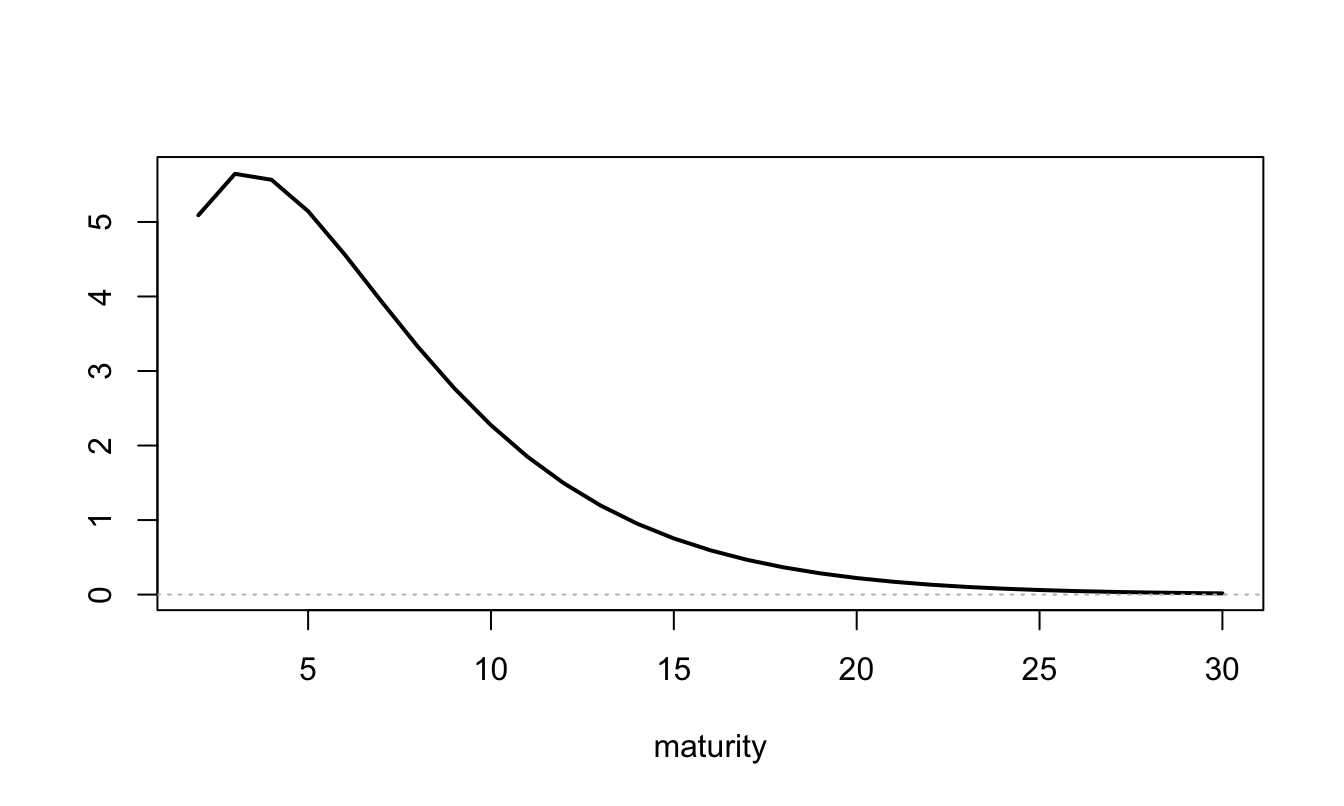
\includegraphics[width=0.95\linewidth]{TSM_files/figure-latex/VV1-1} \caption{Specification of the $\beta_{n,2}$, $n\ge 2$, that specify the influence of the supply factor ($f_{2,t}$) on bond supplies (the $s_{n,t}$'s).}\label{fig:VV1}
\end{figure}

Let us solve the model. Once it is done, let us determine the values of \(\alpha_1\) and \(\beta_1\) that guarantee that \(\sum_n z_{n,t}=1\) (see the discussion above):

\begin{Shaded}
\begin{Highlighting}[]
\NormalTok{RES }\OtherTok{\textless{}{-}} \FunctionTok{solve\_model}\NormalTok{(model,}\AttributeTok{indic.print =} \ConstantTok{FALSE}\NormalTok{)}
\NormalTok{alpha1 }\OtherTok{\textless{}{-}}\NormalTok{ RES}\SpecialCharTok{$}\NormalTok{lambdas}\SpecialCharTok{$}\NormalTok{alpha1}
\NormalTok{beta1  }\OtherTok{\textless{}{-}}\NormalTok{ RES}\SpecialCharTok{$}\NormalTok{lambdas}\SpecialCharTok{$}\NormalTok{beta1}
\NormalTok{Alpha[}\DecValTok{1}\NormalTok{] }\OtherTok{\textless{}{-}}\NormalTok{ alpha1}
\NormalTok{Beta[}\DecValTok{1}\NormalTok{,] }\OtherTok{\textless{}{-}}\NormalTok{ beta1}
\FunctionTok{plot}\NormalTok{(}\DecValTok{1}\SpecialCharTok{:}\NormalTok{N,Beta[}\DecValTok{1}\SpecialCharTok{:}\NormalTok{N,}\DecValTok{2}\NormalTok{],}\AttributeTok{type=}\StringTok{"l"}\NormalTok{,}\AttributeTok{lwd=}\DecValTok{2}\NormalTok{,}\AttributeTok{xlab=}\StringTok{"maturity"}\NormalTok{,}\AttributeTok{ylab=}\StringTok{""}\NormalTok{)}
\end{Highlighting}
\end{Shaded}

\begin{figure}
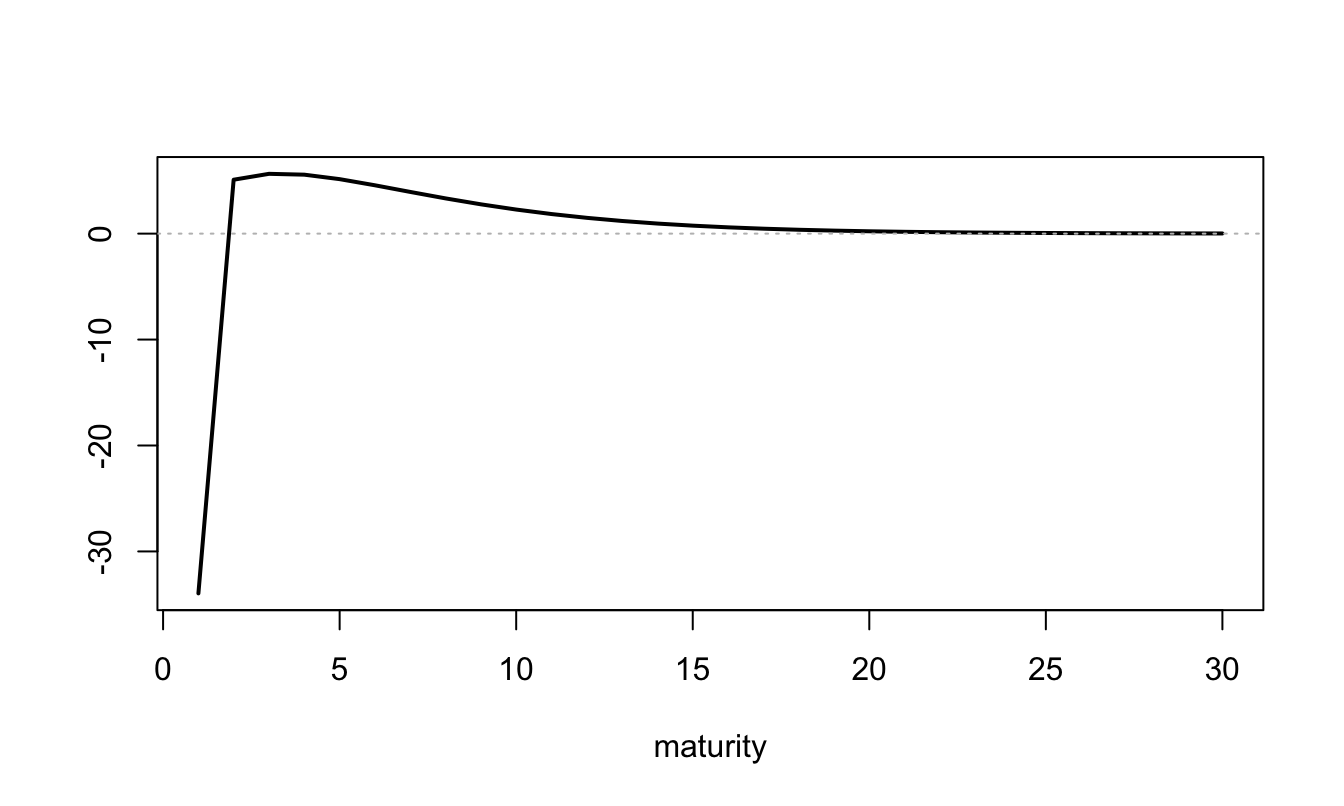
\includegraphics[width=0.95\linewidth]{TSM_files/figure-latex/VV2-1} \caption{Specification of the $\beta_{n,2}$, $n\ge 1$, that specify the influence of the supply factor ($f_{2,t}$) on bond supplies (the $s_{n,t}$'s).}\label{fig:VV2}
\end{figure}

Figure \ref{fig:VV3} shows the two term structures of factor loadings resulting from the model solution.

\begin{Shaded}
\begin{Highlighting}[]
\FunctionTok{par}\NormalTok{(}\AttributeTok{mfrow=}\FunctionTok{c}\NormalTok{(}\DecValTok{1}\NormalTok{,m))}
\ControlFlowTok{for}\NormalTok{(i }\ControlFlowTok{in} \DecValTok{1}\SpecialCharTok{:}\NormalTok{m)\{}
  \FunctionTok{plot}\NormalTok{(}\SpecialCharTok{{-}}\NormalTok{RES}\SpecialCharTok{$}\NormalTok{AB}\SpecialCharTok{$}\NormalTok{B[,i]}\SpecialCharTok{/}\DecValTok{1}\SpecialCharTok{:}\NormalTok{N,}\AttributeTok{type=}\StringTok{"l"}\NormalTok{,}\AttributeTok{lwd=}\DecValTok{2}\NormalTok{,}\AttributeTok{xlab=}\StringTok{"maturity"}\NormalTok{,}\AttributeTok{ylab=}\StringTok{""}\NormalTok{,}
       \AttributeTok{main =} \FunctionTok{paste}\NormalTok{(}\StringTok{"Factor "}\NormalTok{,i,}\AttributeTok{sep=}\StringTok{""}\NormalTok{))\}}
\end{Highlighting}
\end{Shaded}

\begin{figure}
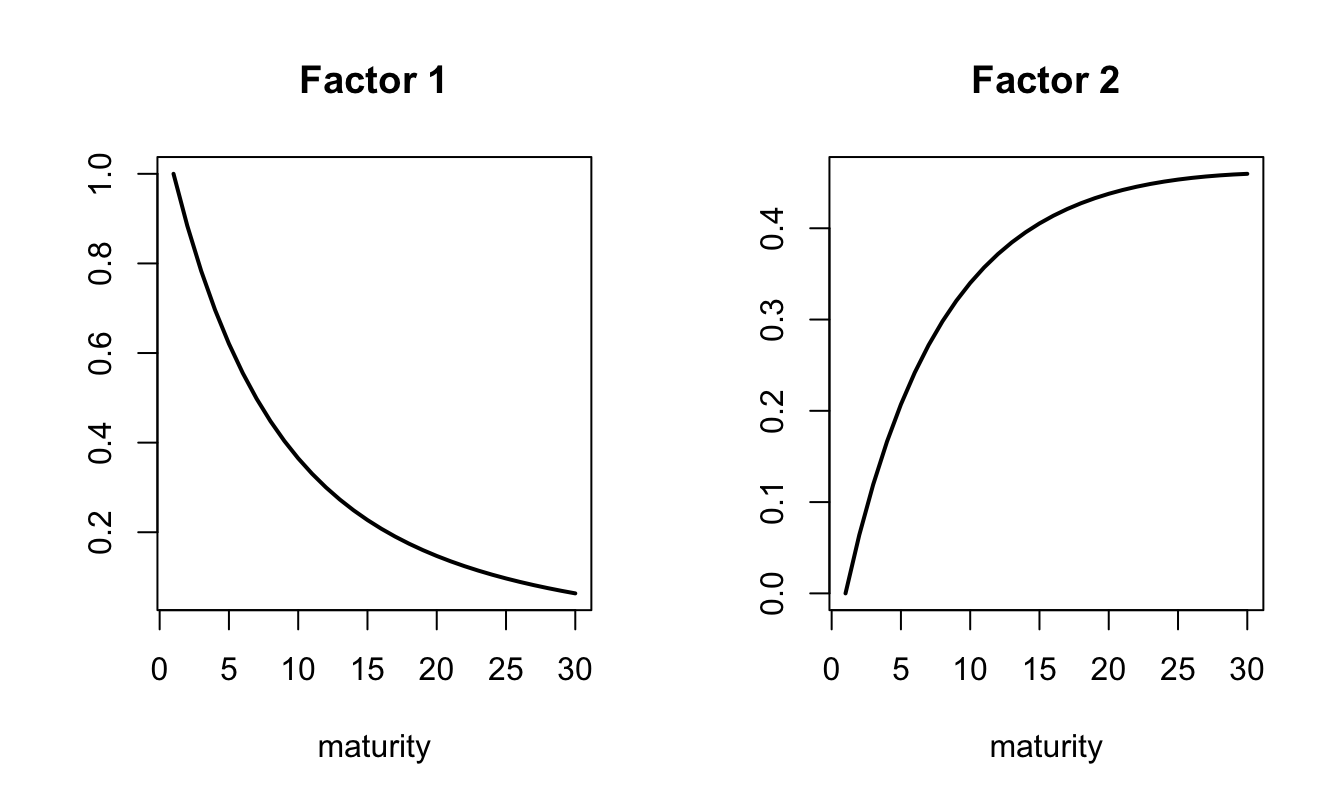
\includegraphics[width=0.95\linewidth]{TSM_files/figure-latex/VV3-1} \caption{Term structure of factor loadings.}\label{fig:VV3}
\end{figure}

Let us know determine the effect of an increase in the supply factor.

\begin{Shaded}
\begin{Highlighting}[]
\CommentTok{\# Shock:}
\NormalTok{shock }\OtherTok{\textless{}{-}} \FunctionTok{matrix}\NormalTok{(}\DecValTok{0}\NormalTok{,m,}\DecValTok{1}\NormalTok{)}
\NormalTok{shock[}\DecValTok{2}\NormalTok{] }\OtherTok{\textless{}{-}}\NormalTok{ .}\DecValTok{01}
\CommentTok{\# baseline yield curve:}
\NormalTok{avg.y      }\OtherTok{\textless{}{-}} \SpecialCharTok{{-}}\NormalTok{ RES}\SpecialCharTok{$}\NormalTok{AB}\SpecialCharTok{$}\NormalTok{A}\SpecialCharTok{/}\NormalTok{(}\DecValTok{1}\SpecialCharTok{:}\NormalTok{N)}
\CommentTok{\# yield curve after shock:}
\NormalTok{shock.y       }\OtherTok{\textless{}{-}} \SpecialCharTok{{-}} \DecValTok{1}\SpecialCharTok{/}\NormalTok{(}\DecValTok{1}\SpecialCharTok{:}\NormalTok{N) }\SpecialCharTok{*}\NormalTok{ (RES}\SpecialCharTok{$}\NormalTok{AB}\SpecialCharTok{$}\NormalTok{A }\SpecialCharTok{+}\NormalTok{ RES}\SpecialCharTok{$}\NormalTok{AB}\SpecialCharTok{$}\NormalTok{B }\SpecialCharTok{\%*\%}\NormalTok{ shock)}
\CommentTok{\# Quantitiies:}
\NormalTok{avg.z   }\OtherTok{\textless{}{-}}\NormalTok{ Alpha }\SpecialCharTok{{-}}\NormalTok{ Zeta }\SpecialCharTok{*}\NormalTok{ avg.y}
\NormalTok{shock.z }\OtherTok{\textless{}{-}}\NormalTok{ Alpha }\SpecialCharTok{+}\NormalTok{ Beta }\SpecialCharTok{\%*\%}\NormalTok{ shock }\SpecialCharTok{{-}}\NormalTok{ Zeta }\SpecialCharTok{*}\NormalTok{ shock.y}

\FunctionTok{par}\NormalTok{(}\AttributeTok{mfrow=}\FunctionTok{c}\NormalTok{(}\DecValTok{1}\NormalTok{,}\DecValTok{2}\NormalTok{))}
\FunctionTok{plot}\NormalTok{(avg.y,}\AttributeTok{type=}\StringTok{"l"}\NormalTok{,}\AttributeTok{ylim=}\FunctionTok{c}\NormalTok{(.}\DecValTok{95}\SpecialCharTok{*}\FunctionTok{min}\NormalTok{(avg.y,shock.y),}\FloatTok{1.05}\SpecialCharTok{*}\FunctionTok{max}\NormalTok{(avg.y,shock.y)),}
     \AttributeTok{lwd=}\DecValTok{2}\NormalTok{,}\AttributeTok{xlab=}\StringTok{"maturity"}\NormalTok{,}\AttributeTok{ylab=}\StringTok{"yields"}\NormalTok{,}\AttributeTok{las=}\DecValTok{1}\NormalTok{)}
\FunctionTok{lines}\NormalTok{(shock.y,}\AttributeTok{lty=}\DecValTok{2}\NormalTok{,}\AttributeTok{lwd=}\DecValTok{2}\NormalTok{,}\AttributeTok{col=}\StringTok{"red"}\NormalTok{)}

\FunctionTok{plot}\NormalTok{(avg.z,}\AttributeTok{ylim=}\FunctionTok{c}\NormalTok{(}\FunctionTok{min}\NormalTok{(avg.z,shock.z),}\FloatTok{1.1}\SpecialCharTok{*}\FunctionTok{max}\NormalTok{(avg.z,shock.z)),}\AttributeTok{pch=}\DecValTok{19}\NormalTok{,}
     \AttributeTok{xlab=}\StringTok{"maturity"}\NormalTok{,}\AttributeTok{ylab=}\StringTok{"Fraction of portfolio"}\NormalTok{,}\AttributeTok{las=}\DecValTok{1}\NormalTok{)}
\FunctionTok{points}\NormalTok{(shock.z,}\AttributeTok{lty=}\DecValTok{2}\NormalTok{,}\AttributeTok{col=}\StringTok{"red"}\NormalTok{,}\AttributeTok{lwd=}\DecValTok{2}\NormalTok{)}
\FunctionTok{abline}\NormalTok{(}\AttributeTok{h=}\DecValTok{0}\NormalTok{,}\AttributeTok{col=}\StringTok{"grey"}\NormalTok{,}\AttributeTok{lty=}\DecValTok{3}\NormalTok{)}
\end{Highlighting}
\end{Shaded}

\begin{figure}
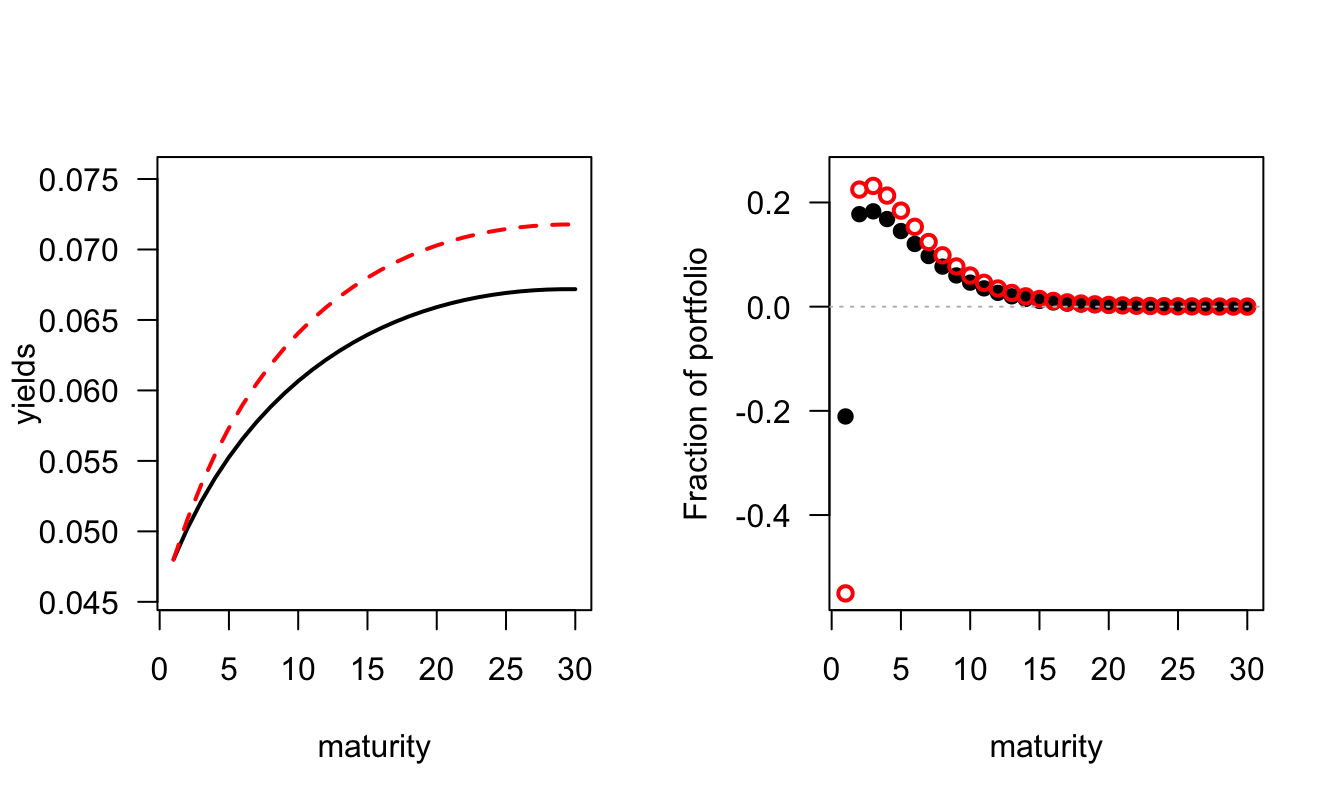
\includegraphics[width=0.95\linewidth]{TSM_files/figure-latex/VV4-1} \caption{Effect of a shock on the second factor. The left hand side plot shows the yield curve effect; the right hand side plot shows the effect on the composition of arbitrageurs' bond portfolio. For the two plots, the black lines indicate the unconditional average and the red line shows the curves conditional on the shock.}\label{fig:VV4}
\end{figure}

\hypertarget{appendix}{%
\section{Appendix}\label{appendix}}

\hypertarget{SDFEZ}{%
\subsection{SDF in the CES Epstein-Zin Context}\label{SDFEZ}}

We denote by \(\pi_t(x_{t+1})\) the price of an asset that provides the payoff \(x_{t+1}\) at date \(t+1\) (as of date \(t\), this payoff may be random). If one purchases \(\varepsilon\) units of this asset and consumes them at date \(t+1\), the intertemporal utility becomes \(F(C_t\color{blue}{ - \varepsilon \pi_t(x_{t+1})},R_t(F(C_{t+1}+\color{blue}{\varepsilon x_{t+1}},R_{t+1}(U_{t+2}))))\).

If \(\pi_t(x_{t+1})\) is the equilibrium price of the asset, then agents should be indifferent between buying a small amount of this asset and not. That is, we should have:
\[
F(C_t,R_t(F(C_{t+1},R_{t+1}(U_{t+2})))) =
F(C_t {\color{blue} - \varepsilon \pi_t(x_{t+1})},R_t(F(C_{t+1}+{\color{blue}\varepsilon x_{t+1}},R_{t+1}(U_{t+2})))).
\]
Let's compute the first-order Taylor expansion of right-hand side term w.r.t. \(\varepsilon\). To begin with, we have:
\[
F(C_{t+1}+{\color{blue}\varepsilon x_{t+1}},R_{t+1}(U_{t+2})) = U_{t+1} + \varepsilon x_{t+1} (1-\beta) C_{t+1}^{-\rho}U_{t+1}^\rho + o(\varepsilon).
\]
Now,
\[
F(C_{t+1}+{\color{blue}\varepsilon x_{t+1}},R_{t+1}(U_{t+2}))^{1-\gamma} = U_{t+1}^{1-\gamma} + \varepsilon x_{t+1}  (1-\beta) C_{t+1}^{-\rho}U_{t+1}^{\rho-\gamma} + o(\varepsilon).
\]
Then,
\[
\mathbb{E}_t \left( F(C_{t+1}+{\color{blue}\varepsilon x_{t+1}},R_{t+1}(U_{t+2}))^{1-\gamma} \right)^{\frac{1}{1-\gamma}}=R_t(U_{t+1}) + \varepsilon R_t(U_{t+1})^{\gamma} \mathbb{E}_t \left(  x_{t+1} (1-\beta) C_{t+1}^{-\rho} U_{t+1}^{\rho-\gamma} \right).
\]
Therefore, \(F(C_t{\color{blue} - \varepsilon \pi_t(x_{t+1})},R_t(F(C_{t+1}+{\color{blue}\varepsilon x_{t+1}},R_{t+1}(U_{t+2}))))\) is equal to \(F(C_t,R_t(U_{t+1}))+\)
\[
\varepsilon R_t(U_{t+1})^{\gamma - \rho} \mathbb{E}_t \left(  x_{t+1} (1-\beta) C_{t+1}^{-\rho} U_{t+1}^{\rho-\gamma} \right) U_t^{\rho}
- \varepsilon \pi_t(x_{t+1}) (1-\beta) C_t^{-\rho} U_t^{\rho} + o(\varepsilon),
\]
which gives \eqref{eq:SS}.

\hypertarget{pricing-and-risk-neutral-dynamics}{%
\chapter{Pricing and risk-neutral dynamics}\label{pricing-and-risk-neutral-dynamics}}

\hypertarget{PricingAAO}{%
\section{SDF: Absence of Arbitrage Approach}\label{PricingAAO}}

Consider a period of interest \({\mathcal T} = \{0,1,2,...,T^*\}\). As in Chapter \ref{ChapterAffine}, vector \(w_t\) constitutes the new information in the economy at \(t\). The historical, or physical, dynamics of \(w_t\), \(f(\underline{w_t})\), is defined by \(f(w_{t+1}|\underline{w_t})\). The physical probability is denoted by \(\mathbb{P}\). \(L_{2t}, t \in {\mathcal T}\), is the (Hilbert) space of square integrate functions \(g(\underline{w_t})\), and we have \(L_{2t} \subset L_{2s}, t< s\).

\hypertarget{existence-and-unicity-of-the-sdf}{%
\subsection{Existence and unicity of the SDF}\label{existence-and-unicity-of-the-sdf}}

\begin{hypothesis}[Price existence and uniqueness]
\protect\hypertarget{hyp:Apricing1}{}\label{hyp:Apricing1}For any \(\underline{w_t}\), there exists a unique \(p_t[g(\underline{w_s})]\),
function of \(\underline{w_t}\), price at \(t\) of a payoff
\(g(\underline{w_s})\) delivered at \(s, \forall t \le s\).
\end{hypothesis}

\begin{hypothesis}[Linearity and continuity]
\protect\hypertarget{hyp:Apricing2}{}\label{hyp:Apricing2}

For all \(t < s\), \(\underline{w_t}\), \(g_1\), \(g_2\), we have

\begin{itemize}
\tightlist
\item
  \(p_t[\lambda_1 g_1(\underline{w_s}) + \lambda_2g_2(\underline{w_s})] = \lambda_1p_t[g_1(\underline{w_s})]+\lambda_2 p_t[g_2(\underline{w_s})]\),
\item
  If \(g_n(\underline{w_s}) \overset{L_{2s}}{\underset{n\rightarrow\infty}{\longrightarrow}} 0\), then \(p_t[g_n(\underline{w_s})] \underset{n\rightarrow\infty}{\longrightarrow} 0\).
\end{itemize}

\end{hypothesis}

\begin{hypothesis}[Absence of Arbitrage Opportunity (AAO)]
\protect\hypertarget{hyp:Apricing3}{}\label{hyp:Apricing3}

At any \(t\), it is impossible to constitute a portfolio of future payoffs, possibly modified at subsequent dates, such that:

\begin{itemize}
\tightlist
\item
  the price of the portfolio at \(t\) is zero,
\item
  payoffs at subsequent dates are \(\ge 0\),
\item
  there is at least one subsequent date \(s\) such that the net payoff at \(s\) is strictly positive with a non zero conditional probability at \(t\).
\end{itemize}

\end{hypothesis}

\begin{theorem}[Riesz representation theorem]
\protect\hypertarget{thm:Riesz}{}\label{thm:Riesz}Under Assumptions \ref{hyp:Apricing1} and \ref{hyp:Apricing2}, for all \(\underline{w_t}\), and \(s > t\), there exists \(\mathcal{M}_{t,s}(\underline{w_s}) \in L_{2s}\), unique such that, \(\forall g(\underline{w_s}) \in L_{2s}\),
\[
p_t[g(\underline{w_s})] = \mathbb{E}[\mathcal{M}_{t,s}(\underline{w_s})g(\underline{w_s})|\underline{w_t}].
\]
In particular the price at \(t\) of a zero coupon bond maturing at \(s\) is \(\mathbb{E}(\mathcal{M}_{t,s}|\underline{w_t})\).
\end{theorem}

\begin{proposition}[Positivity of M]
\protect\hypertarget{prp:PositivityM}{}\label{prp:PositivityM}If Assumption \ref{hyp:Apricing3} is satisfied, then for all \(t\) and \(s\), \(\mathbb{P}(\mathcal{M}_{t,s}>0|\underline{w_t})=1\).
\end{proposition}

\begin{proof}
\(\Leftarrow\) is obvious. If \(\Rightarrow\) was not true, the payoff
\(\textbf{1}_{\{\mathcal{M}_{t,s} \le 0\}}\), at \(s\), would be such that:
\(\mathbb{P}[\textbf{1}_{\{\mathcal{M}_{t,s} \le 0\}}=1|\underline{w_t}] > 0\) and \(p_t[\textbf{1}_{\{\mathcal{M}_{t,s} \le 0\}}] = \mathbb{E}_t[\mathcal{M}_{t,s}\textbf{1}_{\{\mathcal{M}_{t,s} \le 0\}}] \le 0\).
\end{proof}

\begin{proposition}[Time consistency]
\protect\hypertarget{prp:timeconsist}{}\label{prp:timeconsist}

For all \(t < r < s\), we have \(\mathcal{M}_{t,s} = \mathcal{M}_{t,r} \mathcal{M}_{r,s}\), which implies:

\begin{itemize}
\tightlist
\item
  \(\mathcal{M}_{t,s} = \mathcal{M}_{t,t+1} \mathcal{M}_{t+1,t+2}\dots\mathcal{M}_{s-1,s}\)
\item
  \(\mathcal{M}_{0,t} = \Pi^{t-1}_{j=0} \mathcal{M}_{j,j+1}\) (\(\mathcal{M}_{0,t}\) is called \textbf{pricing kernel}).
\end{itemize}

\end{proposition}

\begin{proof}
Using Lemma \ref{lem:sdf} we have:
\begin{eqnarray*}
p_t(g_s) &=& \mathbb{E}(\mathcal{M}_{t,s}g_s|\underline{w_t}) = \mathbb{E}(\mathcal{M}_{t,r} p_r(g_s)|\underline{w_t}) \\
&=& \mathbb{E}[\mathcal{M}_{t,r}\mathbb{E}(\mathcal{M}_{r,s} g_s|\underline{w_r})|\underline{w_t}] = \mathbb{E}(\mathcal{M}_{t,r} \mathcal{M}_{r,s} g_s|\underline{w_t}), \forall g, \forall \underline{w}_{t}
\end{eqnarray*}
and, therefore, \(\mathcal{M}_{t,s} = \mathcal{M}_{t,r}\mathcal{M}_{r,s}\).
\end{proof}

\begin{lemma}
\protect\hypertarget{lem:sdf}{}\label{lem:sdf}For any payoff \(g_s\) at \(s, p_t(g_s) = p_t[p_r(g_s)]\).
\end{lemma}

\begin{proof}
If this was not true, we could construct a sequence of portfolios with a strictly positive payoff at \(s\) with zero payoff at any other future date and with price zero at \(t\), contradicting Assumption \ref{hyp:Apricing3}. Indeed, assuming, for instance, \(p_t(g_s) > p_t[p_r(g_s)]\), the payoff at \(s\) is defined by the following strategy: (i) at \(t\): buy \(p_r(g_s)\), (short) sell \(g_s\), buy
\(\frac{p_t(g_s)-p_t[p_r(g_s)]}{\mathbb{E}(\mathcal{M}_{t,s}|\underline{w_t})}\) zero-coupon bonds maturing at \(s\), at global price zero, (ii) at \(r\): buy \(g_s\) and sell \(p_r(g_s)\), generating a zero net payoff, (iii) at \(s\), the net payoff is: \(g_s-g_s+\frac{p_t(g_s)-p_t[p_r(g_s)]}{\mathbb{E}(\mathcal{M}_{t,s}|\underline{w_t})} > 0\).
\end{proof}

Consider an asset whose payoff, on date \(s\), is \(g(\underline{w_s})\). We have, \(\forall t < s\):
\begin{equation}
\boxed{p_t[g(\underline{w_s})] = \mathbb{E}_t[\mathcal{M}_{t,t+1}...\mathcal{M}_{s-1,s}g(\underline{w_s})].}\label{eq:basic}
\end{equation}
In particular, since \(L_{2,t+1}\) contains 1, the price at \(t\) of a zero-coupon with residual maturity one is given by:
\[
B(t,1) := \mathbb{E}_t [\mathcal{M}_{t,t+1}].
\]
Denoting by \(r_t\) the continously-compounded interest rate, defined through \(B(t,1)=\exp(-r_{t})\), we get
\[
r_{t}=-\log \mathbb{E}_t [\mathcal{M}_{t,t+1}].
\]

\begin{definition}[Bank account]
\protect\hypertarget{def:bankaccount}{}\label{def:bankaccount}The bank account process \(R_t\) is defined by \(R_{t} \equiv \exp(r_0+...+r_{t-1}) = \frac{1}{\mathbb{E}_0[ \mathcal{M}_{0,1}]\times ... \times \mathbb{E}_{t-1} [\mathcal{M}_{t-1,t}]}\).

\(R_t\) is the price of an investment initiated on date 0, when it was worth one dollar, and invested on each date at the risk-free rate (for one period).
\end{definition}

For any price process \(p_t\), we have \(p_t = \mathbb{E}_t(\mathcal{M}_{t,s} p_s)\) (with \(s>t\)), or \(\mathcal{M}_{0,t} p_t = \mathbb{E}_t(\mathcal{M}_{0,s}p_s)\). That is, \(\mathcal{M}_{0,t} p_t\) is a martingale. In particular \(\mathcal{M}_{0,t} R_t\) is a martingale.

\hypertarget{PricingAffine}{%
\subsection{Exponential affine SDF}\label{PricingAffine}}

A specific (tractable) case is that of exponential affine SDF. Assume that
\[
\mathcal{M}_{t,t+1}(\underline{w_{t+1}}) = \exp[\alpha_t(\underline{w_t})'w_{t+1}+\beta_t(\underline{w_t})]
\]
where \(\alpha_t\) defines the \emph{prices of risk} or \emph{sensitivity} vector. Using \(\mathbb{E}_t[\mathcal{M}_{t,t+1}]=\exp(-r_{t})=\exp[\psi_t(\alpha_t)+\beta_t]\), we get:
\begin{equation}
\mathcal{M}_{t,t+1} = \exp[-r_{t}+\alpha'_tw_{t+1}-\psi_t(\alpha_t)].\label{eq:keySDF}
\end{equation}

\begin{example}[CCAPM/Power utility case]
In the CCAPM-power-utility case (see Example \ref{exm:CCAPM}), we have (Eq. \eqref{eq:powerutilSDF}):
\[
\mathcal{M}_{t,t+1} = \exp(\log \delta + \log q_t + \gamma \log   C_t - \log   q_{t+1} - \gamma  \log   C_{t+1}),
\]
where \(q_t\) is the price of the consumption good, \(C_t\) is the quantity consumed at \(t\) and \(\delta\) is the intertemporal discount rate.

Hence, in that case, \(\mathcal{M}_{t,t+1}\) is exponential affine in \(w_{t+1} = (\log q_{t+1}, \log C_{t+1})'\) (and its first lag).
\end{example}

\hypertarget{PricingRN}{%
\section{The risk-neutral (R.N.) dynamics}\label{PricingRN}}

The historical Dynamics is characterized by \(f(\underline{w_{T^*}})\), or by the
sequence of conditional p.d.f. \(f_{t+1}(w_{t+1}|\underline{w_t})\), or
\(f_{t+1}(w_{t+1})\), with respect to (w.r.t.) some measure \(\mu\).

We define the conditional risk-neutral p.d.f. w.r.t. the conditional historical probability. For that, we employ the Radon-Nikodym derivative \(d^{\mathbb{Q}}_{t+1}(w_{t+1}|\underline{w_t})\):\footnote{Of course, the conditional historical p.d.f. with respect to the conditional risk-neutral (R.N.) p.d.f. is:
  \(d_{t+1}(w_{t+1}) = \frac{1}{d^{\mathbb{Q}}_{t+1}(w_{t+1})}\) or \(d_{t+1}(w_{t+1}) = \frac{\exp(-r_{t})}{\mathcal{M}_{t,t+1}}\).}
\[
d^{\mathbb{Q}}_{t+1}(w_{t+1}|\underline{w_t}) =
\frac{\mathcal{M}_{t,t+1}(\underline{w_{t+1}})}{\mathbb{E}[\mathcal{M}_{t,t+1}(\underline{w_{t+1}})|\underline{w_t}]},
\]
or
\[
d^{\mathbb{Q}}_{t+1}(w_{t+1})=
\frac{\mathcal{M}_{t,t+1}}{\mathbb{E}_t(\mathcal{M}_{t,t+1})}=\exp(r_{t}) \mathcal{M}_{t,t+1}.
\]
In this context, the risk neutral conditional p.d.f. is:
\begin{eqnarray}
f^{\mathbb{Q}}_{t+1}(w_{t+1}) &=& f_{t+1}(w_{t+1})d^{\mathbb{Q}}_{t+1}(w_{t+1}) \nonumber \\
&=&f_{t+1} (w_{t+1}) \mathcal{M}_{t,t+1} (\underline{w_{t+1}}) \exp [r_{t} (\underline{w_t})].\label{eq:fQfP}
\end{eqnarray}

The p.d.f. of \(\mathbb{Q}\) w.r.t. the historical dynamics \(\mathbb{P}\) is:
\[
\xi_{T^*} =  \frac{d\mathbb{Q}}{d\mathbb{P}} =
\Pi^{T^{*}-1}_{t=0} d^{\mathbb{Q}}_{t+1}(w_{t+1}) =
\Pi^{T^{*}-1}_{t=0} \exp(r_{t}) \mathcal{M}_{t,t+1},
\]
and the p.d.f. of the R.N. distribution of \(\underline{w_t}\), w.r.t. the corresponding historical distribution is:
\[
\xi_t= \Pi^{t-1}_{\tau=1}
d^{\mathbb{Q}}_{\tau+1}(w_{\tau+1})=\mathbb{E}_t\left(\frac{d\mathbb{Q}}{d\mathbb{P}}\right) = \mathbb{E}_t\xi_{T^*}.
\]
Therefore, \(\xi_t\) is a \(\mathbb{P}\)-martingale.\footnote{Indeed:
  \[
  \mathbb{E}_t \left( \frac{d\mathbb{Q}}{d\mathbb{P}}\right) = \Pi^{t-1}_{\tau = 1} d^{\mathbb{Q}}_{\tau + 1} (w_{\tau+1}) \mathbb{E}_t \left( d^{\mathbb{Q}}_{t+1} (w_{t+1}) \ldots d^{\mathbb{Q}}_{T^*} (w_{T^*})\right).
  \]}

Consider the date-\(t\) price of a payoff \(g(\underline{w_s})\) at time \(s>t\). An equivalent form of the pricing formula \eqref{eq:basic} is:
\begin{eqnarray*}
p_t[g(\underline{w_s})] &=& \mathbb{E}_t[\mathcal{M}_{t,t+1}...\mathcal{M}_{s-1,s}g(\underline{w_s})] \\
&=& \mathbb{E}^{\mathbb{Q}}_t[\exp(-r_{t}-...-r_{s-1})g(\underline{w_s})],
\end{eqnarray*}
or, with simpler notations:
\[
p_t = \mathbb{E}^{\mathbb{Q}}_t[\exp(-r_{t}-...-r_{s-1})p_s] = \mathbb{E}^{\mathbb{Q}}_t\left(\frac{R_t}{R_s} p_s\right),
\]
where \(R_t\) is the \emph{bank account}.

We also have \(p_t/R_t = \mathbb{E}^{\mathbb{Q}}_t\left( p_s/R_s\right)\), that is, \(p_t/R_t\) is a \(\mathbb{Q}\)-martingale. In particular \(p_t = \exp(-r_{t})\mathbb{E}^{\mathbb{Q}}_t(p_{t+1})\), or, using the arithmetic return of any payoff \((p_{t+1}-p_t)/p_t\), and the arithmetic return of the riskless asset \(r_{A,t+1}=\exp(r_{t})-1\), we get:
\[
\mathbb{E}^{\mathbb{Q}}_t\left(\frac{p_{t+1}-p_t}{p_t}\right)=r_{A,t}.
\]
Moreover the excess arithmetic return process \((p_{t+1}-p_t)/p_t-r_{A,t}\) is a \(\mathbb{Q}\)-martingale difference and, therefore, \(\mathbb{Q}\)-serially uncorrelated.

Let us consider the case of an exponential affine SDF \(\mathcal{M}_{t,t+1}=\exp(\alpha'_t w_{t+1}+\beta_t)\):
\[
d^{\mathbb{Q}}_{t+1}(w_{t+1}) = \frac{\mathcal{M}_{t,t+1}}{\mathbb{E}_t(\mathcal{M}_{t,t+1})} = \frac{\exp(\alpha'_t
w_{t+1}+\beta_t)}{\exp[\psi_t(\alpha_t)+\beta_t]} = \exp[\alpha'_t w_{t+1}-\psi_t(\alpha_t)]
\]
We then have that \(d^{\mathbb{Q}}_{t+1}(w_{t+1})\) is also exponential affine. Moreover:
\[
f^{\mathbb{Q}}_{t+1} (w_{t+1}) = \frac{f_{t+1} (w_{t+1}) \exp (\alpha'_t w_{t+1})}{\varphi_t (\alpha_t)}.
\]
The previous equation shows that \(f^{\mathbb{Q}}_{t+1}\) is the Esscher transform of \(f_{t+1}\) evaluated at \(\alpha_t\).

Let us know consider the Laplace transform of the conditional R.N. probability, \(\varphi^{\mathbb{Q}}_t(u|\underline{w_t})\), also denoted by \(\varphi^{\mathbb{Q}}_t(u)\). We have:
\begin{eqnarray*}
\varphi^{\mathbb{Q}}_t(u) &=& \mathbb{E}^{\mathbb{Q}}_t \exp(u' w_{t+1}) \\
&=& \mathbb{E}_t \exp[(u+\alpha_t)'w_{t+1}-\psi_t(\alpha_t)] \\
&=& \exp[\psi_t(u+\alpha_t)-\psi_t(\alpha_t)] =
\frac{\varphi_t(u+\alpha_t)}{\varphi_t(\alpha_t)}.
\end{eqnarray*}
Hence:
\begin{equation}
\boxed{\psi^{\mathbb{Q}}_t(u) = \psi_t(u+\alpha_t)-\psi_t(\alpha_t).}\label{eq:transfoPQ}
\end{equation}
We check that, if \(\alpha_t=0\), \(\psi^{\mathbb{Q}}_t=\psi_t\) (since \(\psi_t(0)=0)\).

Moreover, putting \(u=-\alpha_t\) in the expression of
\(\psi^{\mathbb{Q}}_t(u)\) we get \(\psi^{\mathbb{Q}}_t(-\alpha_t)=-\psi_t(\alpha_t)\),
and, replacing \(u\) by \(u-\alpha_t\), we get:
\[
\boxed{\psi_t(u) = \psi^{\mathbb{Q}}_t(u-\alpha_t)-\psi^{\mathbb{Q}}_t(-\alpha_t).}
\]
Also:
\begin{equation*}
\left\{
\begin{array}{ccl}
d_{t+1}(w_{t+1}) &=& \exp[-\alpha'_t(w_{t+1})-\psi^{\mathbb{Q}}_t(-\alpha_t)] \\
d^{\mathbb{Q}}_{t+1}(w_{t+1}) &=& \exp[\alpha'_t(w_{t+1})+\psi^{\mathbb{Q}}_t(-\alpha_t)].
\end{array}
\right.
\end{equation*}

\hypertarget{PricingTypology}{%
\section{Typology of econometric asset-pricing models}\label{PricingTypology}}

\begin{definition}[Econometric Asset Pricing Model (EAPM)]
\protect\hypertarget{def:typo}{}\label{def:typo}

An Econometric Asset Pricing Model (EAPM) is defined by the following functions:

\begin{itemize}
\tightlist
\item
  \(r_{t}(\underline{w_t})\),
\item
  \(f(w_{t+1}|\underline{w_t}))\) {[}or \(\psi_t(u)\){]},
\item
  \(\mathcal{M}_{t,t+1}(\underline{w_{t+1}})\),
\item
  \(f^{\mathbb{Q}}(w_{t+1}|\underline{w_t})\) {[}or \(\psi^{\mathbb{Q}}_t(u)\){]}.
\end{itemize}

\end{definition}

The previous functions have to to be specified and parameterized. They are linked by:
\[
f^{\mathbb{Q}}(w_{t+1}|\underline{w_t}) = f(w_{t+1}|\underline{w_t}) \mathcal{M}_{t,t+1}(\underline{w_{t+1}}) \exp[r_{t}(\underline{w_t}))].
\]

In the following, we present three ways of specifying an EAPM:

\begin{enumerate}
\def\labelenumi{\arabic{enumi}.}
\tightlist
\item
  the direct modelling,
\item
  the R.N.-constrained direct modelling (or mixed modelling),
\item
  the back modelling.
\end{enumerate}

We focus on the case where \(\mathcal{M}_{t,t+1}\) is exponential affine, as in Eq. \eqref{eq:keySDF}:
\[
\mathcal{M}_{t,t+1} (\underline{w_{t+1}}) = \exp\left\{ -r_{t} (\underline{w_t}) + \alpha'_t(\underline{w_t})w_{t+1} - \psi_t [\alpha_t (w_t)]\right\}.
\]
Once the short-term rate function \(r_{t}(\underline{w_t})\) is specified, we have to specify \(\psi_t\), \(\alpha_t\), and \(\psi^{\mathbb{Q}}_t\), that are linked by Eq. \eqref{eq:transfoPQ}.

In all approaches, we have to specify the status of the short rate. The short rate \(r_{t}\) is a function of \(\underline{w_t}\), this function may be known or unknown by the econometrician. It is known in two cases: (a) \(r_{t}\) is exogenous (\(r_{t}(\underline{w_t})\) does not depend on \(\underline{w_t}\)) or (b) \(r_{t}\) is a component of \(w_t\). By contrast, if the function \(r_{t} (\underline{w_t})\) is unknown, it has to be specified parametrically:
\[
\left\{ r_{t} (\underline{w_t}, \tilde{\theta}), \tilde{\theta}\in \tilde{\Theta} \right\},
\]
where \(r_{t}(\bullet,\bullet)\) is a known function.

Let us now detail the three steps on which each of the three ways of defining an EAPM is based.

\hypertarget{DirectModeling}{%
\subsection{The direct modelling}\label{DirectModeling}}

\begin{itemize}
\tightlist
\item
  \textbf{Step 1 -- Specification of the historical dynamics}. We choose a parametric family for the conditional historical Log-Laplace transform \(\psi_t(u|\underline{w_t})\): \(\left\{ \psi_t (u|\underline{w_t} ; \theta_1), \theta_1 \in \Theta_1 \right\}\).
\item
  \textbf{Step 2 -- Specification of the SDF}. Considering the affine specification of as Eq. \eqref{eq:keySDF}, that is:
  \[
  \mathcal{M}_{t,t+1} (\underline{w_{t+1}}) = \exp\left\{ -r_{t}(\underline{w_t}, \tilde{\theta}) + \alpha'_t(\underline{w_t})w_{t+1} - \psi_t [\alpha_t (w_t)|\underline{w_t} ; \theta_1]\right\},
  \]
  we need to specifiy functions \(r_{t}(\underline{w_t}, \tilde{\theta})\) and \(\alpha_t(\underline{w_t})\). Assume that \(\alpha_t(\underline{w_t})\) belongs to a parametric family: \(\left\{ \alpha_t (\underline{w_t} ; \theta_2),\theta_2 \in \Theta_2 \right\}\).
  We then have:
  \begin{eqnarray*}
  \mathcal{M}_{t,t+1}(\underline{w_{t+1}}, \theta) &=& \exp \left\{ - r_{t}
  (\underline{w_t}, \tilde{\theta}) + \alpha'_t (\underline{w_t},\theta_2) w_{t+1} - \psi_{t} \left[ \alpha_t (\underline{w_t},
  \theta_2) | \underline{w_t} ; \theta_1 \right] \right\},
  \end{eqnarray*}
  where \(\theta = (\tilde{\theta}', \theta'_1,\theta'_2)' \in \tilde{\Theta}\times \Theta_1 \times \Theta_2 = \Theta\).
\item
  \textbf{Step 3 -- Internal consistency conditions (ICC)}. For any payoff \(g(\underline{w_s})\) settled at \(s>t\), with price \(p(\underline{w_t})\) at \(t\) which is a known function of
  \(\underline{w_t}\), we must have:
  \begin{equation*}
  p(\underline{w_t}) = \mathbb{E} \left\{\mathcal{M}_{t,t+1} (\theta) \dots \mathcal{M}_{s-1,s} (\theta) g(\underline{w_s})  |  \underline{w_t},
  \theta_1 \right\}    \forall \; \underline{w_t}, \theta.\label{eq:ICCgen}
  \end{equation*}
  These ICC pricing conditions may imply strong constraints on \(\theta\). For instance, when components of \(w_t\) are returns of some assets: if \(w_{1,t} = \log(p_{1,t}/p_{1,t-1})\), then we must have \(\mathbb{E}_t [\mathcal{M}_{t,t+1} \exp (e'_1 w_{t+1})]= 1\) (Euler equation). Or, in the case of interest rates with various maturities: if \(w_{1,t} = -1/h\log B(t,h)\), then we must have \(e'_1 w_{t} = - 1/h \log \mathbb{E}_t (\mathcal{M}_{t,t+1}\times \dots \times \mathcal{M}_{t+h-1,t+h})\).
\end{itemize}

The previous three steps imply the specification of the R.N. dynamics (according to Eq. \eqref{eq:transfoPQ}):
\begin{equation*}
\psi^{\mathbb{Q}} (u | \underline{w_t}, \theta_1, \theta_2) =
\psi_t \left[ u + \alpha_t (\underline{w_t}, \theta_2) |
\underline{w_t}, \theta_1 \right] - \psi_t \left[ \alpha_t
(\underline{w_t}, \theta_2) | \underline{w_t}, \theta_1
\right].
\end{equation*}

\hypertarget{the-r.n.-constrained-direct-modelling-or-mixed-modelling}{%
\subsection{The R.N.-constrained direct modelling (or mixed modelling)}\label{the-r.n.-constrained-direct-modelling-or-mixed-modelling}}

\begin{itemize}
\tightlist
\item
  \textbf{Step 1 -- Specification of the physical dynamics}. We select a family \(\{ \psi_t (u | \underline{w_t},\theta_1), \theta_1 \in \Theta_1 \}\).
\item
  \textbf{Step 2 -- Specification of the risk-neutral dynamics}. We select a family \(\{\psi^{\mathbb{Q}}_t (u | \underline{w_t}, \theta^*),\theta^* \in \Theta^* \}\) and, possibly, \(\{r_{t}(\underline{w_t},\tilde{\theta}),\tilde{\theta}\in\tilde{\Theta}\}\).
\item
  \textbf{Step 3 -- Internal Consistency Conditions (ICC)}. Once the parameterization \((\tilde{\theta}, \theta_1, \theta^*) \in \tilde{\Theta} \times \Theta^*_1\) is defined, ICCs may be imposed. For instance, if \(w_{1,t} = \log(p_{1,t}/p_{1,t-1})\), then we must have \(\exp(-r_t)\mathbb{E}^{\mathbb{Q}}_t \exp (e_{1}' w_{t+1}) = 1\). Or if \(w_{1,t} = B(t,h)\), then \(e_{1}' w_{t} = \mathbb{E}_t^{\mathbb{Q}} \exp(-r_t - \dots - r_{t+h-1})\).
\end{itemize}

The SDF is a by-product. If we want an exponential affine SDF, for any pair \((\psi^{\mathbb{Q}}_t, \psi_t)\) belonging to these families, there must exist a unique function \(\alpha_t (\underline{w_t})\) denoted by \(\alpha_t (w_t ; \theta_1, \theta^*)\), and satisfying:
\begin{equation*}
\psi^{\mathbb{Q}}_t (u | \underline{w_t}) = \psi_t \left[ u +
\alpha_t (w_t) | \underline{w_t} \right] - \psi_t \left[
\alpha_t (\underline{w_t}) | \underline{w_t} \right].
\end{equation*}

\hypertarget{back-modelling-based-on-three-steps}{%
\subsection{Back modelling (based on three steps)}\label{back-modelling-based-on-three-steps}}

\begin{itemize}
\tightlist
\item
  \textbf{Step 1 -- Specification of the R.N. dynamics}, and possibly of \(r_{t}(\underline{w_t})\){]}: \(\psi^{\mathbb{Q}}_t (u | \underline{w_t}; \theta^*_1)\).
\item
  \textbf{Step 2 -- Internal consistency conditions (ICC)}, if relevant, are taken into account:
  \begin{equation*}
  \begin{array}{lll}
  && p(\underline{w_t}) = \mathbb{E}^{\mathbb{Q}}_t \left[ \exp (-r_{t} (\underline{w_t},\tilde{\theta}) - \dots - r_{s-1} (\underline{w_s}, \tilde{\theta}))g(\underline{w_s}) | \underline{w_t} , \theta^*_1\right] ,\\
  && \forall    \underline{w_t} , \tilde{\theta} , \theta^*_1.
  \end{array}
  \end{equation*}
\item
  \textbf{Step 3 -- Choice of the specification of the prices of risk}. One chooses function \(\alpha_t(\underline{w_t})\) without any constraint; this amounts to defining the family \(\{ \alpha_t (\underline{w_t}, \theta^*_2), \theta^*_2\in \Theta^*_2 \}\).
\end{itemize}

The historical dynamics is obtained as a by-product. Indeed:
\begin{equation*}
\psi_t(u | \underline{w_t} ; \theta^*_1, \theta^*_2) = \psi_t^{\mathbb{Q}}\left[ u -\alpha_t (\underline{w_t}, \theta^*_2)|\underline{w_t} ; \theta^*_1 \right] -\psi^{\mathbb{Q}}_t \left[- \alpha_t (\underline{w_t}, \theta^*_2) | \underline{w_t},\theta^*_1 \right].
\end{equation*}

\hypertarget{the-term-structure-or-risk-free-yields}{%
\chapter{The term structure or risk-free yields}\label{the-term-structure-or-risk-free-yields}}

\hypertarget{RFIntroduction}{%
\section{Introduction}\label{RFIntroduction}}

Risk-free yields are the yields-to-maturity associated with bonds that carry no default and/or liquidity risks. Bonds issued by sovereign entities with top credit quality are usually considered to be risk-free.

An important share of the term-structure literature pertains to the modelling of risk-free yields. Some models involve macro factors in \(w_t\) \citep{Ang_Piazzesi_2003}; some do not \citep{Duffie_Singleton_1997}. The latter are sometimes called \emph{yield-only} models.

The basic pricing formula of a risk-free zero coupon bond is (see Eq. \eqref{eq:stdbond} in Example \ref{exm:nominalBth}):
\begin{eqnarray}
B(t,h) &=& \exp(-r_{t}) \mathbb{E}^{\mathbb{Q}}_t \exp(-r_{t+1}-\dots-r_{t+h-1})\\
R(t,h) &=& - \frac{1}{h} \log B(t,h). \label{eq:stdbondRFchapter}
\end{eqnarray}

Term structure models are often used to extract \emph{term premiums} from observed yields-to-maturity. Term premiums are those components of yields that would not exist if investors were not risk-averse.

If agents were not risk averse, i.e., under the \emph{Expectation Hypothesis (EH)}, we would have \(\mathcal{M}_{t,t+1} = \exp(- r_t)\). We would then have \(\mathbb{P} \equiv \mathbb{Q}\) and \(B(t,h)\) would become:
\begin{equation}
\exp(-r_{t}) \mathbb{E}_t \exp(-r_{t+1}-\dots-r_{t+h-1}).\label{eq:stdbondRFchapterP}
\end{equation}
And the maturity-\(h\) yield-to-maturity would then be:
\begin{eqnarray}
R^{EH}(t,h) &=& -\frac{1}{h}\log \left( \mathbb{E}_t \exp(-r_t-\dots-r_{t+h-1})\right)\nonumber\\
&\approx& \frac{1}{h}\mathbb{E}_t(r_t + \dots + r_{t+h-1}).\label{eq:REH}
\end{eqnarray}

The term premium is given by:
\begin{eqnarray}
TP_{t,h} &=& \underbrace{- \frac{1}{h} \log  \mathbb{E}^{\mathbb{Q}}_t \exp(-r_{t+1}-\dots-r_{t+h-1})}_{=R(t,h)} - \nonumber \\
&& \underbrace{- \frac{1}{h}  \log  \mathbb{E}_t \exp(-r_{t+1}-\dots-r_{t+h-1}).}_{=R^{EH}(t,h)}\label{eq:TP}
\end{eqnarray}

What is the economic meaning of the term premium? Under EH, investors are willing to buy a maturity-\(h\) bond as long as its expected return is---up to Jensen's inequality---equal to the average of future short-term rates. (Hence the definition of \(R^{EH}(t,h)\), see Eq. \eqref{eq:REH}.) When \(TP_{t,h}>0\), investors are willing to buy the maturity-\(h\) bond only if its return is, on average, higher than expected future short-term rates; this corresponds to a situation where investors consider that long-term bonds tend to lose value in \emph{bad states of the world} (i.e., states of high marginal utility).

\begin{quote}
\textbf{\emph{Risk premium:}} According to Eq. \eqref{eq:Mbasicpricing}, the price of any asset \(j\) satisfies:
\[
p_{jt} = \mathbb{E}_t(\mathcal{M}_{t,t+1} p_{j,t+1}).
\]
The previous equation rewrites:
\[
p_{jt} =  \mathbb{C}ov_t(\mathcal{M}_{t,t+1}, p_{j,t+1}) + \mathbb{E}_t(\mathcal{M}_{t,t+1})\mathbb{E}_t( p_{j,t+1})
\]
or
\begin{equation}
p_{jt} = \underbrace{\exp(-r_t)\mathbb{E}_t( p_{j,t+1})}_{=p^{EH}_{jt}} + \underbrace{\mathbb{C}ov_t(\mathcal{M}_{t,t+1}, p_{j,t+1})}_{\mbox{Risk premium}}.\label{eq:CovRP}
\end{equation}
If investors were not risk-averse, then we would have \(p_{jt} = p^{EH}_{jt}\). The S.D.F. is high (resp. low) in bad (resp. good) states of the world (states of high marginal utility in the equilibrium approach). Hence, we have \(p_{jt}< p^{EH}_{jt}\) if asset \(j\) tends to pay less in bad states of the world (i.e., if \(\mathbb{C}ov_t(\mathcal{M}_{t,t+1}, p_{j,t+1})<0\)).
\end{quote}

Bonds issued by top-rated (Aaa/AAA) countries are often considered to be risk-free. Because of call-margins mechanisms, swap rates are also used as risk-free benchmarks \citep{Duffie_Stein_2015} (see Subsection \ref{Swaps}).

If agents were risk-neutral, we would have:
\[
B_{t,n} = \exp(-R_{t,m})\mathbb{E}_t(B_{t+m,n-m}).
\]
This would imply:
\[
-n R_{t,n} = -R_{t,m} + \log \mathbb{E}_t[\exp(-(n-m) R_{t+m,n-m})].
\]
Up to the Jensen inequality, and taking expectations on both sides, we get:
\[
-n R_{t,n} \approx \mathbb{E}_t(-R_{t,m} -(n-m) R_{t+m,n-m}).
\]
After having reorganized:
\begin{equation}
\mathbb{E}_t(R_{t+m,n-m}-R_{t,n}) \approx \frac{R_{t,n}-R_{t,m}}{n-m}.\label{eq:CStheo}
\end{equation}

\citet{Campbell_Shiller_1991} have used the previous expression to test for the Expectation hypothesis. Formally, they run the following regressions for different values of \(n\) and \(m\):
\[
R_{t+m,n-m}-R_{t,n}) = \phi_n\frac{R_{t,n}-R_{t,m}}{n-m} + \varepsilon_{t+m}
\]

According to \eqref{eq:CStheo}, under the Expectation Hypothesis, we should have \(\phi_{n,m} \approx 1\). But they do find that the \(\phi_{n,m}\) are statistically lower than one. Besides, they find that, for a given holding period \(m\), the term structure of the \(\phi_{n,m}\) decreases with the maturity \(n\). Figure \ref{fig:CSregressions} shows

\textbackslash begin\{figure\}
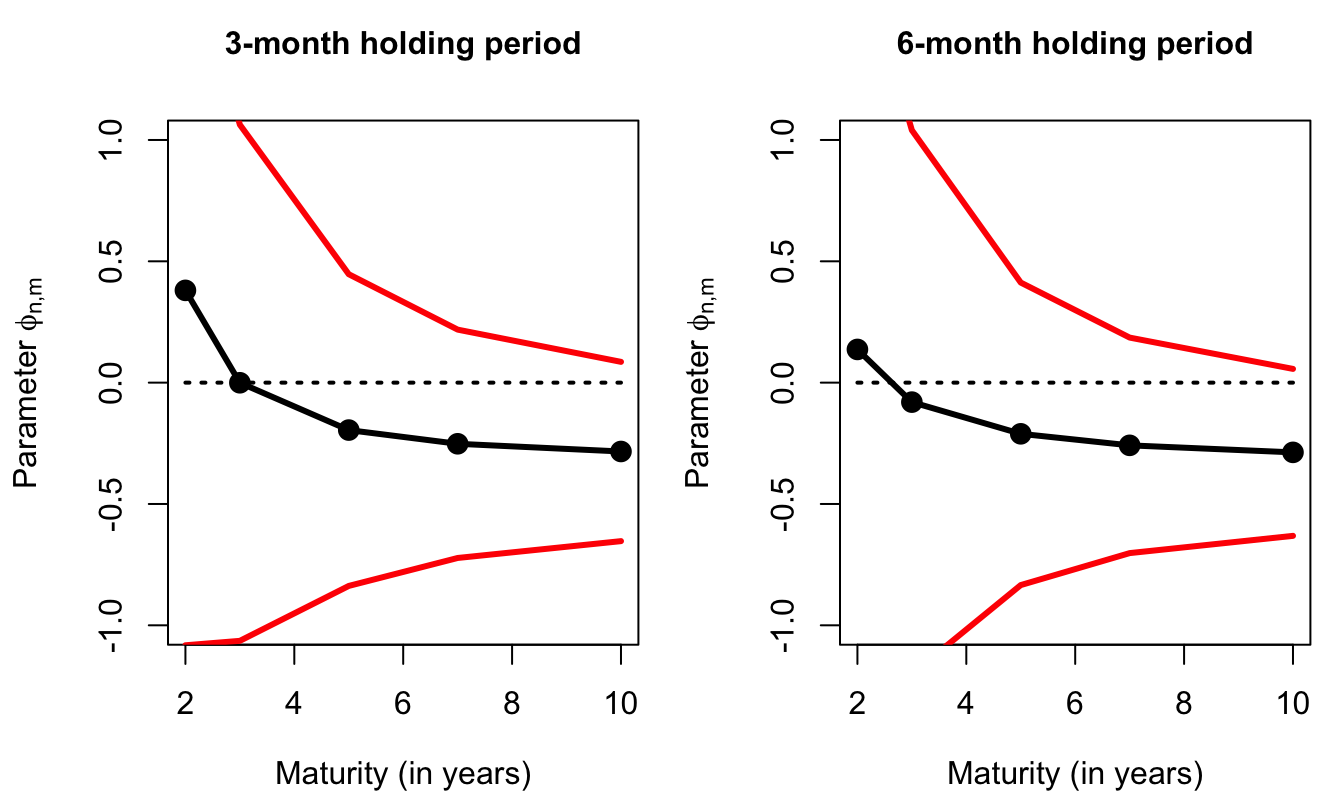
\includegraphics[width=0.95\linewidth]{TSM_files/figure-latex/CSregressions-1} \textbackslash caption\{Regressions as in Campbell and Shiller (1991). Data are at the monthly frequency; they are collected from the FRED database. The estimation period starts in 1990. The figure reports 90\% confidence intervals of the \(\phi_{n,m}\) parameter estimates (Newey-West robust standard deviations).\}\label{fig:CSregressions}
\textbackslash end\{figure\}

\hypertarget{RiskFreeAffine}{%
\section{The Affine Case}\label{RiskFreeAffine}}

\hypertarget{affine-yields}{%
\subsection{Affine yields}\label{affine-yields}}

In this subsection, we consider the case where the state vector \(w_t\) is affine under both \(\mathbb{P}\) and \(\mathbb{Q}\). If the nominal short-term rate is affine in \(w_t\), i.e., if \(r_t = \omega_0 + \omega'_1 w_t\), then:
\begin{eqnarray*}
B(t,h) &=& \mathbb{E}^{\mathbb{Q}}_t \exp (-r_{t}-\dots-r_{t+h-1})\\
&=& \exp(-h\omega_0 - \omega'_1 w_t) \color{blue}{\mathbb{E}^{\mathbb{Q}}_t \exp (- \omega'_1 w_{t+1}-\dots- \omega'_1 w_{t+h-1})}.
\end{eqnarray*}
The (blue) expectation is easily computed using the recursive equations of Lemma \ref{lem:MHLT} (see Example \ref{exm:nominalBth}), leading to:
\begin{equation}
R(t,h)= -  \frac{1}{h}   \log   B(t,h) = A_h'w_t + B_h.\label{eq:RthAB}
\end{equation}
It is easily seen that we can also get:
\begin{equation}
R^{EH}(t,h) = {A^{EH}_h}'w_t + B^{EH}_h.\label{eq:RthABEH}
\end{equation}
Moreover, if inflation is also affine in \(w_t\), i.e., if \(\pi_{t} = \bar\omega_0 + \bar\omega'_1 w_t\), then real yields are given by:
\begin{eqnarray*}
\bar{B}(t,h) &=& \mathbb{E}^{\mathbb{Q}}_t \exp(-r_{t}-\dots-r_{t+h-1}+\pi_{t+1}+\dots+\pi_{t+h})
\end{eqnarray*}
(see Example \ref{exm:realBth}) which also leads to:
\begin{equation}
\bar{R}(t,h) = -  \frac{1}{h}   \log   \bar{B}(t,h) = \bar{A}_h'w_t + \bar{B}_h.\label{eq:RbarthAB}
\end{equation}
Eqs. \eqref{eq:RthAB} and \eqref{eq:RthABEH} imply that term premiums are affine in \(w_t\) (see Eq. \eqref{eq:TP}). Specifically:
\[
TP(t,h) = R(t,h) - E^{EH}(t,h) = B_h - B_h^{EH} + (A_h - A_h^{EH})'w_t.
\]
Expected excess returns resulting from holding zero-coupon bonds are also affine in \(w_t\). Indeed, holding a maturity-\(h\) zero-coupon bond for one period provides the following expected gross return:
\[
\mathbb{E}_t\left(\frac{B(t+1,h-1)}{B(t,h)}\right) = \mathbb{E}_t\left(\exp(B_{h-1} - B_h + A_{h-1}'w_{t+1} - A_h'w_{t})\right),
\]
which is clearly exponential affine in \(w_t\) if \(w_t\) is an affine process. Therefore, the expected excess return, that is:
\[
\log \mathbb{E}_t\left(\frac{B(t+1,h-1)}{B(t,h)}\right) - r_t
\]
is also affine in \(w_t\) in this context. The fact that excess returns are affine in this context is exploited in the estimation approach proposed by \citet{Adrian_Crump_Moench_2013}.

Moreover, \emph{conditional expectations} of future interest rates (real or nominal) and of term premiums are also affine in \(w_t\). In particular:
\begin{equation}
\mathbb{E}_t[R(t+k,h)] = \mathbb{E}_t[{A_h}'w_{t+k} + B_h] = {A_h}'\mathbb{E}_t(w_{t+k}) + B_h,\label{eq:condmeanRth}
\end{equation}
and \(\mathbb{E}_t(w_{t+k})\) is affine in \(w_t\) (see Eq. \eqref{eq:condmean}). This can notably be used at the estimation stage, if one wants to fit survey data (see Section XXX).

Similarly, \emph{conditional variances} of future interest rates (real or nominal) and of term premiums are affine in \(w_t\). In particular:
\begin{equation}
\mathbb{V}ar_t[R(t+k,h)] = \mathbb{V}ar_t[{A_h}'w_{t+k} + B_h] = {A_h}'\mathbb{V}ar_t(w_{t+k})A_h,\label{eq:condvarRth}
\end{equation}
where the components of \(\mathbb{V}ar_t(w_{t+k})\) (and therefore \(\mathbb{V}ar_t[R(t+k,h)]\)) is affine in \(w_t\) (see Eq. \eqref{eq:condvar}). This can also be used at the estimation stage, if one wants to fit (proxies of) conditional variances \citep{zarg_2017}.

\hypertarget{maximum-sharpe-ratio}{%
\subsection{Maximum Sharpe ratio}\label{maximum-sharpe-ratio}}

In an affine model, the maximum Sharpe ratio is easily computed. This has been noted early by \citet{Duffee_2010} for the Gaussian model; \citet{Gourieroux_Monfort_Mouabbi_Renne_2021} and \citet{Pallara_Renne_2023} use it in more sophisticated affine models.

Let us derive the maximum Sharpe ratio in the context of a genral affine framework. Eq. \eqref{eq:CovRP} implies that
\[
\mathbb{E}_t\underbrace{\left(\frac{p_{j,t+1}}{p_{j,t}} - \exp(r_t)\right)}_{=xs_{j,t+1},\mbox{ excess return}} =  - \exp(r_t) \mathbb{C}ov_t\left(\mathcal{M}_{t,t+1},\frac{p_{j,t+1}}{p_{j,t}}\right),
\]
and, using \(|\mathbb{C}ov(X,Y)| \le \sqrt{\mathbb{V}ar(X)\mathbb{V}ar(Y)}\), we get the \citet{Hansen_Jagannathan_1991} bound:
\begin{equation}
\underbrace{\frac{\mathbb{E}_t(xs_{j,t+1})}{\sqrt{\mathbb{V}ar_t(xs_{j,t+1})}}}_{\mbox{Sharpe ratio}} \le \underbrace{\frac{\sqrt{\mathbb{V}ar_t(\mathcal{M}_{t,t+1})}}{\mathbb{E}_t(\mathcal{M}_{t,t+1})}}_{\mbox{Maximum Sharpe ratio}}.
\end{equation}

If the S.D.F. is given by \(\mathcal{M}_{t,t+1} = \exp[-r_{t}+\alpha'_tw_{t+1}-\psi_t(\alpha_t)]\) (Eq. \eqref{eq:keySDF}), and using that \(\mathbb{E}_t(\mathcal{M}_{t,t+1}^2)=\exp(-2r_t+\psi_t(2\alpha_t)-2\psi_t(\alpha_t))\) we get:
\[
\mbox{Maximum Sharpe ratio} = \sqrt{\exp(\psi_t(2\alpha_t)-2\psi_t(\alpha_t)) - 1}.
\]

\hypertarget{RiskFreeGaussian}{%
\section{Gaussian Affine Term Structure Model}\label{RiskFreeGaussian}}

The Gaussian Affine Term Structure Model (GATSM) is a \emph{workhorse} model, widely used in academic and economic-policy circles. In a GATSM, \(w_t\) follows a Gaussian vector autoregressive model, and is therefore affine under \(\mathbb{P}\). The S.D.F. is exponential affine in \(w_t\), which implies that it is also affine under \(\mathbb{Q}\) (see Subsection XXX). Since the components of \(w_t\) are valued in \(\mathbb{R}\), one can easily introduce macro-factors among the state variables.

Let us be more specific. The state vector \(w_t\) follows:
\begin{equation}
w_{t+1} = \mu + \Phi w_{t} + \Sigma^{1/2} \varepsilon_{t+1}, \mbox{ where } \varepsilon_{t} \sim  i.i.d. \mathcal{N}(0,Id).\label{eq:GaussianVAR1}
\end{equation}
(The fact that we consider a VAR(1) process is without loss of generality since a VAR(p) admits a VAR(1) companion representation.)

This implies the following Laplace transform for \(w_t\) (see Example \ref{exm:Gaussian}):
\[
\psi_t(u) = \log \mathbb{E}_t(\exp(u'w_{t+1})|\underline{w_t}) = \color{blue}{u'\mu + u'\Phi w_t + \frac{1}{2}u'\Sigma'u}.
\]
Using the notations of Eq. \eqref{eq:keySDF}, the s.d.f. is defined as:
\[
\mathcal{M}_{t,t+1} = \exp(- r_t + \alpha_t'w_{t+1} - \psi_t(\alpha_t)), \mbox{ where } \alpha_t = \alpha_0 + \alpha_1'w_t.
\]

In that case, using Eq. \eqref{eq:transfoPQ}, we get:
\begin{eqnarray*}
\psi_t^{\mathbb{Q}}(u) &=& \psi_t(u + \alpha_t) - \psi_t(\alpha_t)\\
&=& (u + \alpha_t)'\mu + (u + \alpha_t)'\Phi w_t + \frac{1}{2}(u + \alpha_t)'\Sigma(u + \alpha_t) \\
&& - \left(\alpha_t'\mu + \alpha_t'\Phi w_t + \frac{1}{2}\alpha_t'\Sigma\alpha_t\right) \\
&=& \color{blue}{u' \left(\mu + \Sigma \alpha_0 \right) + u'(\Phi + \Sigma \alpha_1')w_t  + \frac{1}{2}u'\Sigma'u}.
\end{eqnarray*}
The \(\mathbb{Q}\)-dynamics of \(w_t\) is (from Example \ref{exm:Gaussian}):
\[
w_{t+1} = \mu + \Sigma  \alpha_0 + (\Phi + \Sigma \alpha_1')  w_{t} + \Sigma^{1/2} \varepsilon^*_{t+1}, \mbox{ where } \varepsilon^*_{t} \sim  i.i.d. \mathcal{N}^{\mathbb{Q}}(0,Id).
\]
Hence, \(w_t\) also follows a VAR process under \(\mathbb{Q}\) since the previous equation rewrites:
\[
w_{t+1} = \mu^{\mathbb{Q}} + \Phi^{\mathbb{Q}} w_{t} + \Sigma^{1/2} \varepsilon^*_{t+1},
\]
where \(\mu^{\mathbb{Q}} = \mu + \Sigma \alpha_0\) and \(\Phi^{\mathbb{Q}}=\Phi + \Sigma \alpha_1'\).

With affine specifications of the nominal short term rate (\(r_{t} = \omega_0 + \omega'_1 w_t\)) and of the inflation rate (\(\pi_{t} = \bar\omega_0 + \bar\omega'_1 w_t\)), we obtain affine formulas for nominal and real yields of any maturity (Eqs. \eqref{eq:RthAB} and \eqref{eq:RbarthAB}).

\begin{example}[Kim and Wright (2005)]
\protect\hypertarget{exm:KimWright}{}\label{exm:KimWright}

This model is a three-factor \emph{yield-only model} (no macro variables, except inflation in one variant of the model), where the short-term rate reads \(r_t = \omega_0 + \omega_{1,1} w_{1,t} +\omega_{1,2} w_{2,t} +\omega_{1,3} w_{3,t}\).

The model estimated by Kalman filter (see Subsection,\ref{Estimation:KF}; the state-space model (Def. \ref{def:LSSM}) includes survey-based variables (see Subsection \ref{EstimationPersistency}).

Outputs are \href{https://www.federalreserve.gov/pubs/feds/2005/200533/200533abs.html}{regularly updated by the Federal Reserve Board}.

Monthly data on the 6-month and 12-month-ahead forecasts of the three-month T-Bill yield from Blue Chip Financial Forecasts and semiannual data on the average expected three-month T-Bill yield from 6 to 11 years.

\begin{figure}
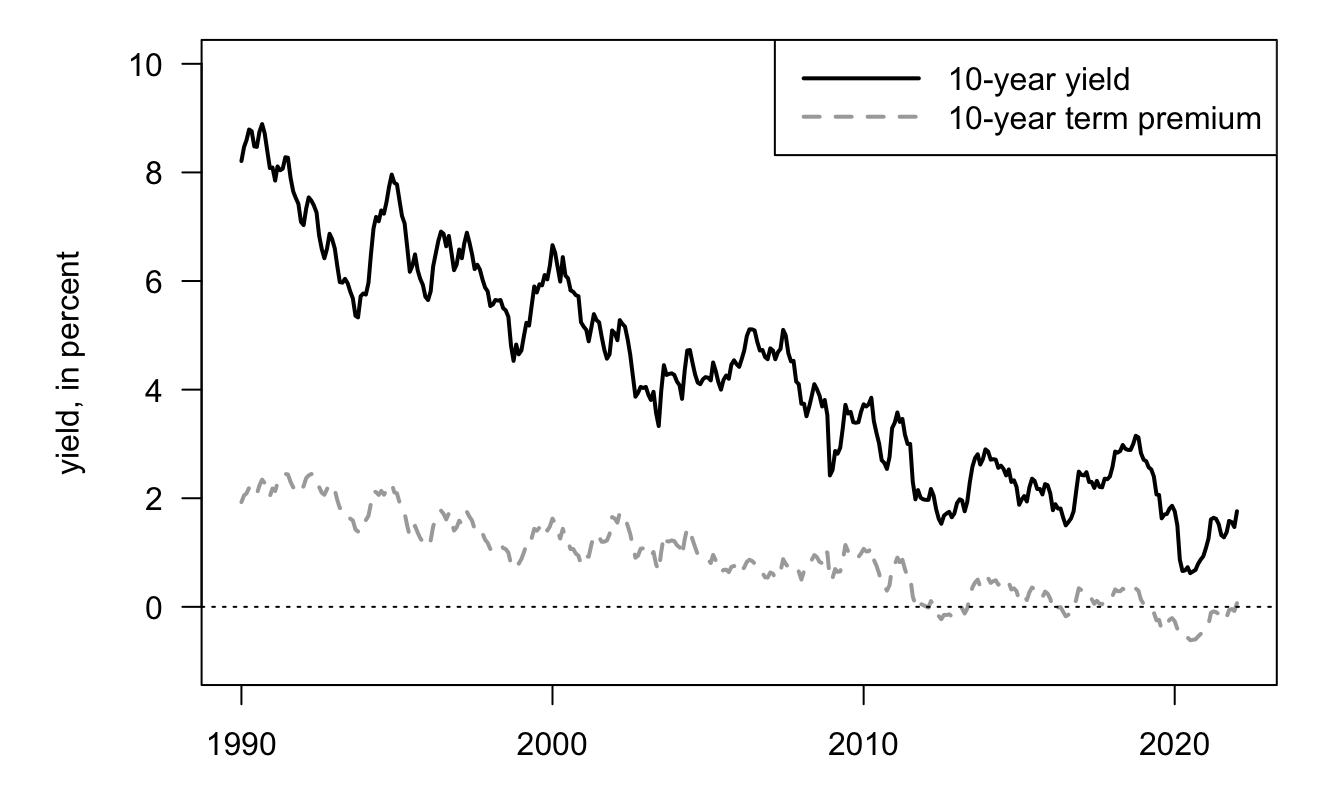
\includegraphics[width=0.95\linewidth]{TSM_files/figure-latex/fredKW-1} \caption{Kim and Wright (2005) outputs.}\label{fig:fredKW}
\end{figure}

\end{example}

\begin{example}[Ang and Piazzesi (2003)]
\protect\hypertarget{exm:AngPiazzesi}{}\label{exm:AngPiazzesi}

\citet{Ang_Piazzesi_2003} propose one of the first paper mixing latent and macrovariables. The set up is also of the form Eq. \eqref{eq:GaussianVAR1}, except that the VAR features several lags.\footnote{Note that a VAR with \(p\) lags (i.e., a VAR(\(p\))) admits a VAR(1) companion form.} In their model, \(w_t = [f^{o}_{1,t},f^{o}_{2,t},f^{u}_{1,t},f^{u}_{2,t},f^{u}_{3,t}]'\) where:

\begin{itemize}
\tightlist
\item
  \(f^{o}_{1,t}\) is the first Principal Component of a set of 3 price indexes (growth rates)
\item
  \(f^{o}_{2,t}\) is the first Principal Component of a set of 4 real activity proxies (HELP, EMPLOY, IP, UE).
\item
  \(f^{u}_{i,t}\) are unobserved, or latent, factors.
\end{itemize}

The nominal short-term rate follows a Taylor rule. And latent factors are estimated via \emph{inversion techniques} (Subsection \ref{EstimationInversion}).

\begin{figure}

{\centering 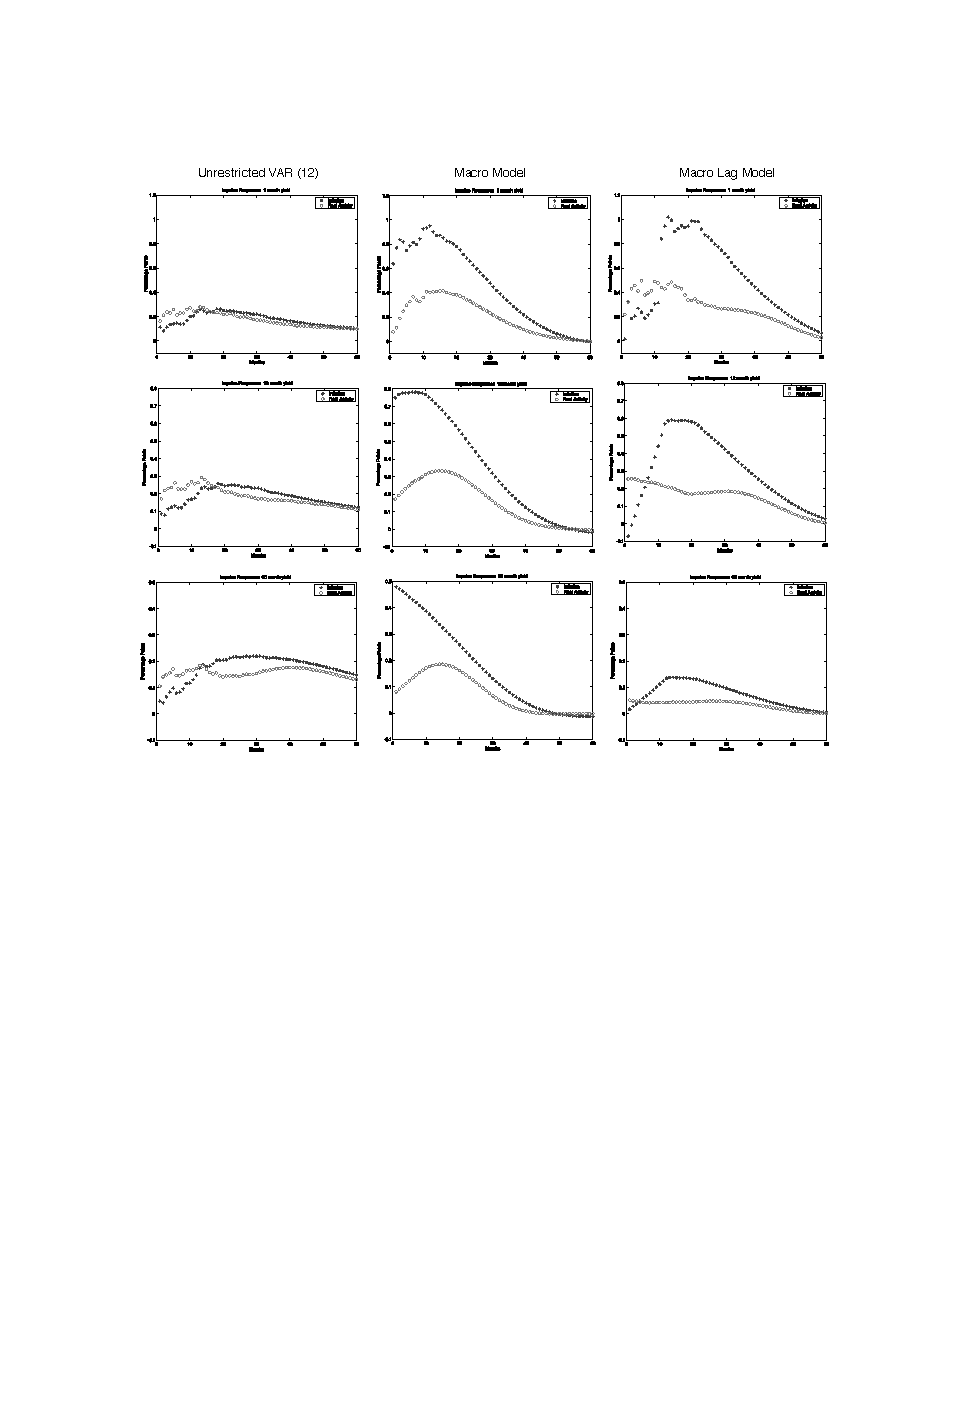
\includegraphics[width=0.95\linewidth]{figures/AngPiazzesi1} 

}

\caption{Source: Ang and Piazzesi (1998). Impulse response functions.}\label{fig:figAngPiazzesi}
\end{figure}

\end{example}

\begin{example}[Joslin, Priebsch and Singleton (2014)]
\protect\hypertarget{exm:JPS}{}\label{exm:JPS}

\citet{Joslin_Priebsch_Singleton_2014} first note that affine models stating that the short term rate is affine in macro factors imply that macro-factors are \emph{spanned} by the yield curve: macro-factors should be perfectly explained by yields of different maturities. Further, they show that this is not the case in the data. (That is, regressing macro factors on yields provides \(R^2\) that are far from one.)

They propose a model where macro factors are unspanned by the yield curve, but can still help predict yields. In their model, \(w_t = [\mathcal{P}_t',M_t']'\), where \(\mathcal{P}_t\) are yield factors (\(\approx\) principal components) and \(M_t\) are macro factors. The model is as follows:
\begin{eqnarray*}
r_t &=& \omega_{0} + \omega_{\mathcal{P}}'\mathcal{P}_t \\
\left[\begin{array}{c}\mathcal{P}_t \\ M_t \end{array}\right]
&=&
\left[\begin{array}{cc}\Phi_{\mathcal{P}\mathcal{P}}&\Phi_{\mathcal{P}M} \\
\Phi_{M\mathcal{P}}&\Phi_{MM} \end{array}\right]
\left[\begin{array}{c}\mathcal{P}_{t-1} \\ M_{t-1} \end{array}\right] + \Sigma \varepsilon_t \\
\left[\begin{array}{c}\mathcal{P}_t \\ M_t \end{array}\right] &=& \mu +
\left[\begin{array}{cc}\Phi^{\mathbb{Q}}_{\mathcal{P}\mathcal{P}}&{\color{red}0} \\
\Phi^{\mathbb{Q}}_{M\mathcal{P}}&\Phi^{\mathbb{Q}}_{MM} \end{array}\right]
\left[\begin{array}{c}\mathcal{P}_{t-1} \\ M_{t-1} \end{array}\right] + \Sigma \varepsilon^{\mathbb{Q}}_t,
\end{eqnarray*}
where \(\varepsilon_t\) and \(\varepsilon^{\mathbb{Q}}_t\) are \(\mathcal{N}(0,Id)\) under \(\mathbb{P}\) and \(\mathbb{Q}\), respectively.

\(M_t\) does Granger-cause \(\mathcal{P}_t\) under \(\mathbb{Q}\) and \(r_t\) is affine in \(\mathcal{P}_t\) (only).

In this context, yields \(R(t,h)\) are affine in \(\mathcal{P}_t\) (only). However \(M_t\) does Granger-cause \(\mathcal{P}_t\) under \(\mathbb{P}\), that is, macro-shocks affect the yield curve.

\begin{figure}

{\centering 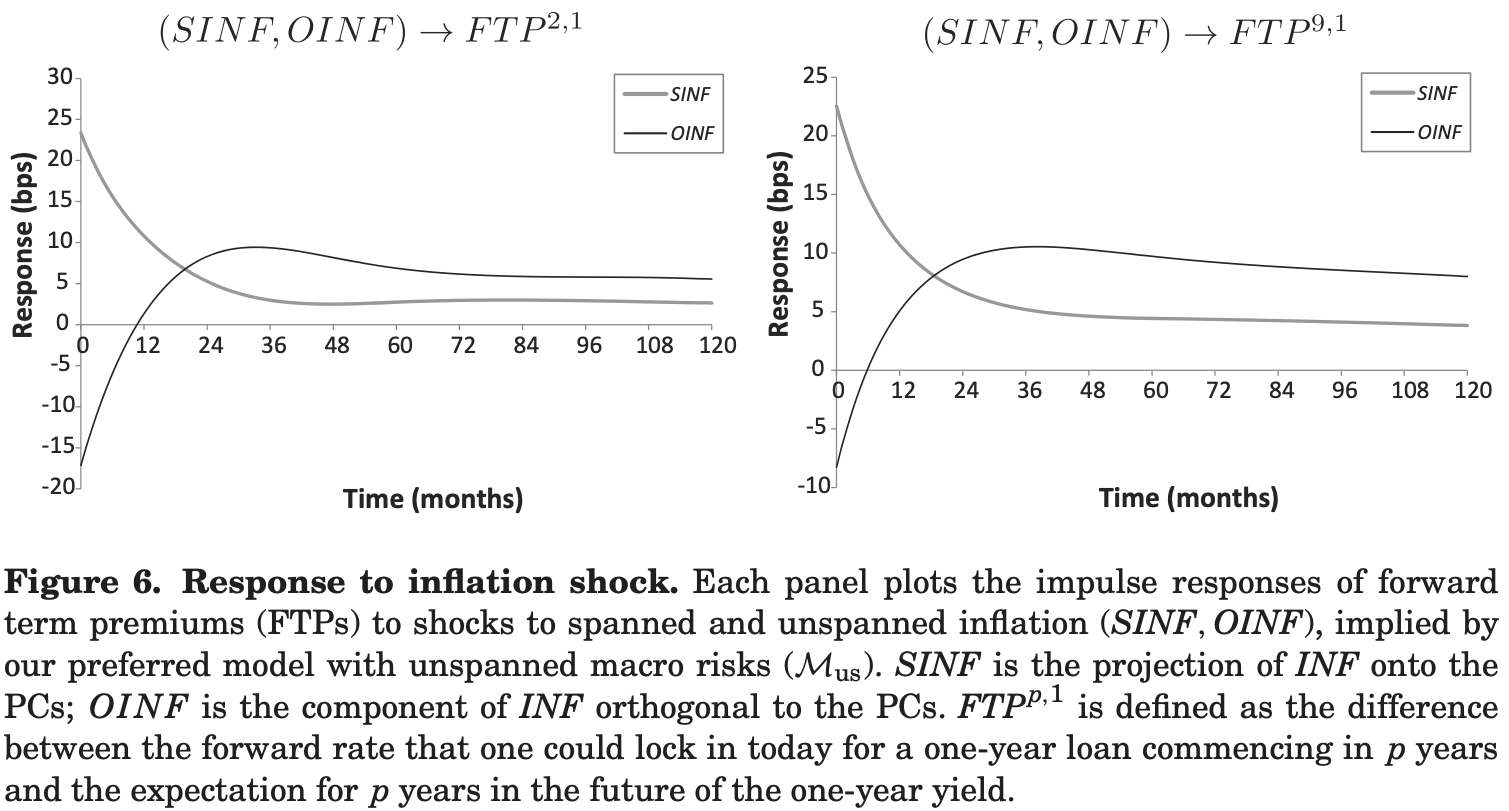
\includegraphics[width=0.95\linewidth]{figures/JPS_IRF} 

}

\caption{Source: Joslin, Priebsch, and Singleton (2014). Impulse response functions.}\label{fig:JPSIRF}
\end{figure}

\end{example}

\begin{example}[Ang, Boivin, Dong and Loo-Kung (2011)]
\protect\hypertarget{exm:Angetal2011}{}\label{exm:Angetal2011}

\citet{Ang_Boivin_Dong_LooKung_2011} propose a macro-finance model based on a quadratic framework. The short-term rate follows a Taylor rule with time-varying parameters:
\[
r_t = \omega_0 + a_t g_t + b_t \pi_t,
\]
where \(x_t=(g_t,\pi_t,a_t,b_t)'\) follows a Gaussian VAR. This is the context described in Example \ref{exm:QGVAR1}. The previous equation shows that \(r_t\) is linear in \(w_t = (x_t,vec(x_t x_t')')'\). Specifically:
\[
r_t = \omega_0 + \omega_1'w_t,
\]
with \(\omega_1 = [v,vec(V)]'\), where
\[
v = \left[
\begin{array}{c}
0\\
0\\
0\\
0
\end{array}
\right] \quad \mbox{and} \quad V = \left[
\begin{array}{cccc}
0 & 0& 1/2&0\\
0& 0& 0&1/2\\
1/2& 0& 0&0\\
0&1/2 &0 &0
\end{array}
\right].
\]

\begin{figure}

{\centering 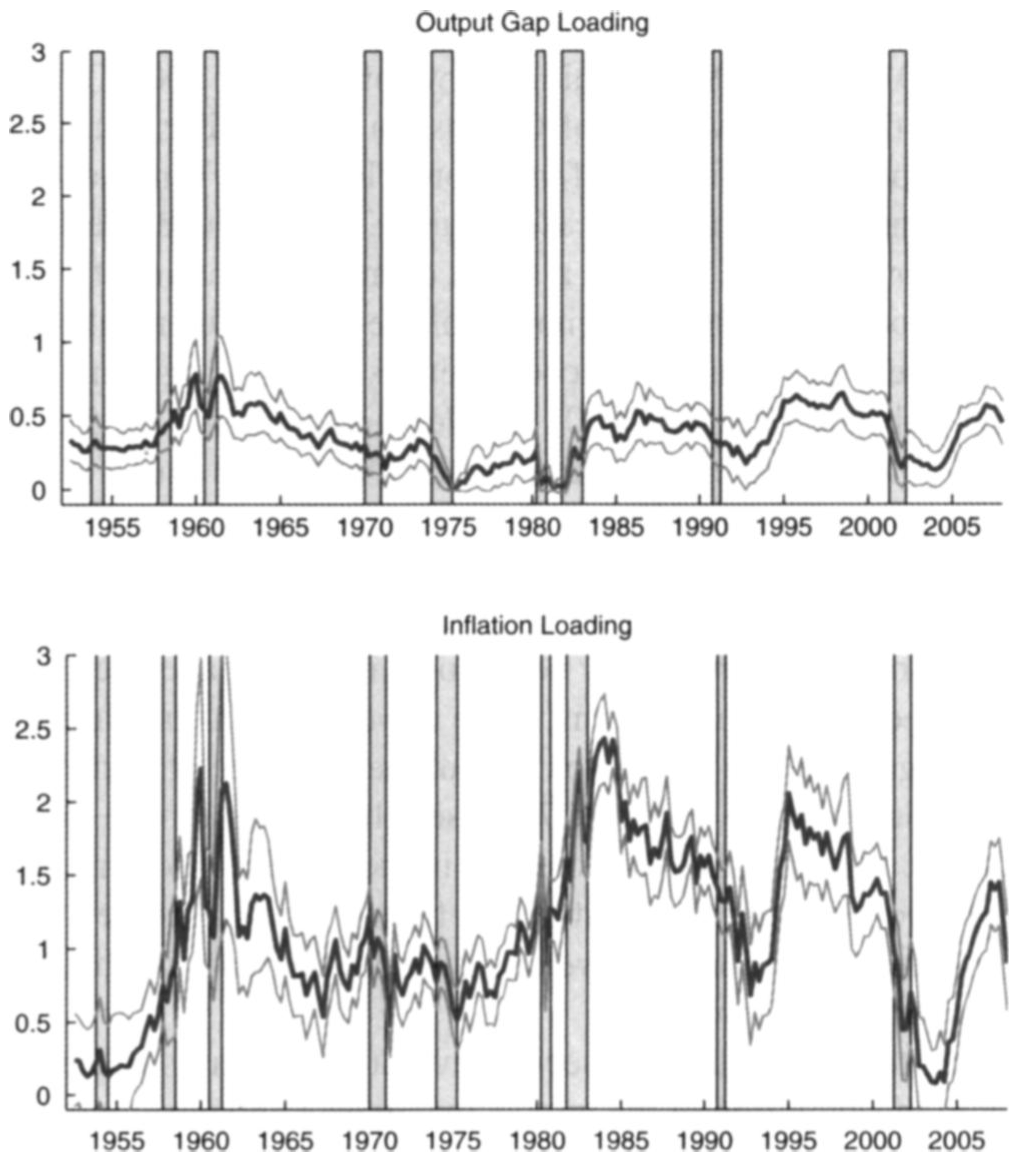
\includegraphics[width=0.7\linewidth]{figures/Ang_Boivin_loadings} 

}

\caption{Source: Ang, Boivin, Dong, Loo-Kung (2011). Estimated factor loadings ($a_t$ and $b_t$).}\label{fig:AngBoivin}
\end{figure}

\end{example}

\hypertarget{RiskFreeNonNegative}{%
\section{Non-Negative Affine Term Structure Model}\label{RiskFreeNonNegative}}

In the presence of physical currency, absence of arbitrage opportunity and of storing cost of cash, nominal interest rates should be nonnegative. Many standard models (e.g.~Gaussian ATSM) are non consistent with non-negative nominal yields. The period of extremely low interest rates challenged these models. Against this backdrop, approaches have been developed to accommodate zero (or effective) lower bounds. We provide two examples; only the second is an affine model.

\hypertarget{the-shadow-rate-approach}{%
\subsection{The shadow-rate approach}\label{the-shadow-rate-approach}}

The shadow-rate model is originally due to \citet{Black_1995}. In this model, the short term rate is given by:
\begin{equation}
r_t = \max(s_t,\underline{r}),\label{eq:SRSTR}
\end{equation}
where \(s_t\) is the shadow short-term interest rate and \(\underline{r}\) is the effective lower bound (\(\le 0\)). While \(s_t\) can be real-valued, the short term rate is nonnegative under \eqref{eq:SRSTR}. In shadow-rate models, the shadow rate \(s_t\) is usually a linear combination of a vector \(w_t\) that follows a Gaussian auto-regressive model. While \(s_t\) is a linear combination of components of an affine process, this is not the case for \(r_t\). As a result, pricing formula are not available in closed-form. Approximation formula have been proposed by, e.g., \citet{Krippner_2013}, \citet{Priebsch_2013}, \citet{Wu_Xia_2016}.

Let us describe the latter approach \citep{Wu_Xia_2016}. As in Subsection \ref{RiskFreeGaussian}, the S.D.F. is defined as:
\[
\mathcal{M}_{t,t+1} = \exp(- r_t + \alpha_t'w_{t+1} - \psi_t(\alpha_t)), \mbox{ where } \alpha_t = \alpha_0 + \alpha_1'w_t,
\]
(this is Eq. \eqref{eq:keySDF}), but the short-term rate \(r_t\) is given by \(r_t = \max(s_t,0)\), with
\[
s_t = \delta_0 + \delta_1' w_t.
\]

The approximation approach proposed by \citet{Wu_Xia_2016} is based on an approximation to the conditional expectations of forward rates. Using the results of Subsection \ref{FWD}, we have (Eq. \eqref{eq:forward}):
\[
f_{n-1,n,t} = n R_{t,n} - (n-1) R_{t,n-1}.,
\]
for \(n>0\) (and using \(R_{t,0}=0\)). This implies that:
\[
R_{t,h} =  \frac{1}{h}(f_{t,0,1}+f_{t,1,2}+\dots+f_{t,h-1,h}).
\]

The approximation of \citet{Wu_Xia_2016} consists in finding approximations of the forward rates \(f_{t,n-1,n}\) (denoted by \(\tilde{f}_{t,n-1,n}\), say) and to use them in the previous equation to get:
\begin{equation}
\boxed{R_{t,h} \approx  \frac{1}{h}\left(\tilde{f}_{t,0,1}+\tilde{f}_{t,1,2}+\dots+\tilde{f}_{t,h-1,h}\right).}\label{eq:RapproxSR}
\end{equation}

Using that, for any random variable \(Z\), we have \(\log(\mathbb{E}[e^Z]) \approx \mathbb{E}[Z] + \frac{1}{2} \mathbb{V}ar[Z]\) (based on a second order Taylor expansion), \citet{Wu_Xia_2016} further show that:
\begin{eqnarray}
f_{t,n,n+1} &=& -\log\left(\mathbb{E}_t^{\mathbb{Q}}\left(e^{-\sum_{j=0}^n r_{t+j}}\right)\right) + \log\left(\mathbb{E}_t^{\mathbb{Q}}\left(e^{-\sum_{j=0}^{n-1} r_{t+j}}\right)\right)\\
&\approx& \mathbb{E}_t^{\mathbb{Q}}[r_{t+n}] - \frac{1}{2}\left(\mathbb{V}ar_t^{\mathbb{Q}}\left(\sum_{j=0}^n r_{t+j}\right)-\mathbb{V}ar_t^{\mathbb{Q}}\left(\sum_{j=0}^{n-1} r_{t+j}\right)\right).
\end{eqnarray}

The expectation can be computed analytically:
\[
\mathbb{E}_t^{\mathbb{Q}}[r_{t+n}] = \underline{r} + \sigma_n^{\mathbb{Q}}g\left(\frac{\bar{a}_n + b_n'X_t - \underline{r}}{\sigma_n^{\mathbb{Q}}}\right),
\]
where \(g(x)= x\Phi(x)-\phi(x)\), \(\Phi\) and \(\phi\) being the c.d.f. and p.d.f. of the standard normal distribution, respectively, and where
\begin{eqnarray*}
\bar{a}_n &=& \delta_0 + \delta_1'\left(\sum_{j=0}^{n-1} \left[\Phi^{\mathbb{Q}}\right]^j\right)\mu^{\mathbb{Q}}\\
b_n' &=& \delta_1'\left(\Phi^{\mathbb{Q}}\right)^n.
\end{eqnarray*}
They also show that
\[
\frac{1}{2}\left(\mathbb{V}ar_t^{\mathbb{Q}}\left(\sum_{j=0}^n r_{t+j}\right)-\mathbb{V}ar_t^{\mathbb{Q}}\left(\sum_{j=0}^{n-1} r_{t+j}\right)\right) \approx \Phi\left(\frac{\bar{a}_n + b_n'X_t - \underline{r}}{\sigma_n^{\mathbb{Q}}}\right)\times(\bar{a}_n - a_n),
\]
where
\[
a_n = \bar{a}_n - \frac{1}{2}\sigma_n^{\mathbb{Q}},
\]
with
\[
\sigma_n^{\mathbb{Q}} := \mathbb{V}ar^{\mathbb{Q}}_t\left(s_{t+n}\right)= \delta_1'\left(\sum_{j=0}^{n-1} \left[\Phi^{\mathbb{Q}}\right]^j\right)\Sigma \Sigma' \left(\sum_{j=0}^{n-1} \left[\Phi^{\mathbb{Q}}\right]^j\right)'\delta_1.
\]
They finally obtain:
\[
\boxed{f_{t,n,n+1} \approx \tilde{f}_{t,n,n+1} = \underline{r} + \sigma_n^{\mathbb{Q}}g\left(\frac{a_n + b_n'X_t - \underline{r}}{\sigma_n^{\mathbb{Q}}}\right),}
\]
which is used in \eqref{eq:RapproxSR} to obtain an approximation to \(R_{t,h}\).

\begin{Shaded}
\begin{Highlighting}[]
\FunctionTok{library}\NormalTok{(TSModels)}
\CommentTok{\# Specify model:}
\NormalTok{n }\OtherTok{\textless{}{-}} \DecValTok{2} \CommentTok{\# number of factors}
\NormalTok{rho }\OtherTok{\textless{}{-}} \FunctionTok{matrix}\NormalTok{(}\DecValTok{0}\NormalTok{,n,n)}
\FunctionTok{diag}\NormalTok{(rho) }\OtherTok{\textless{}{-}}\NormalTok{ .}\DecValTok{97}
\NormalTok{mu }\OtherTok{\textless{}{-}} \FunctionTok{matrix}\NormalTok{(}\DecValTok{0}\NormalTok{,n,}\DecValTok{1}\NormalTok{)}
\NormalTok{Sigma }\OtherTok{\textless{}{-}} \FunctionTok{diag}\NormalTok{(n)}
\NormalTok{delta}\FloatTok{.0} \OtherTok{\textless{}{-}} \DecValTok{0}\NormalTok{;delta}\FloatTok{.1} \OtherTok{\textless{}{-}} \FunctionTok{rep}\NormalTok{(.}\DecValTok{01}\NormalTok{,n)}
\NormalTok{r.bar }\OtherTok{\textless{}{-}} \DecValTok{0} \CommentTok{\# r = max(s,r.bar) [i.e., r.bar=0 in standard model]}
\NormalTok{Model }\OtherTok{\textless{}{-}} \FunctionTok{list}\NormalTok{(}\AttributeTok{rho =}\NormalTok{ rho,}\AttributeTok{mu =}\NormalTok{ mu,}\AttributeTok{Sigma =}\NormalTok{ Sigma,}
              \AttributeTok{delta.0 =}\NormalTok{ delta}\FloatTok{.0}\NormalTok{,}\AttributeTok{delta.1 =}\NormalTok{ delta}\FloatTok{.1}\NormalTok{,}\AttributeTok{r.bar =}\NormalTok{ r.bar)}
\CommentTok{\# Simulate model and compute shadow rate:}
\NormalTok{X }\OtherTok{\textless{}{-}} \FunctionTok{simul.var}\NormalTok{(Model,}\AttributeTok{nb.sim =} \DecValTok{200}\NormalTok{) }\CommentTok{\# simulated path}
\NormalTok{s }\OtherTok{\textless{}{-}}\NormalTok{ delta}\FloatTok{.0} \SpecialCharTok{+}\NormalTok{ X }\SpecialCharTok{\%*\%}\NormalTok{ delta}\FloatTok{.1}
\CommentTok{\# Compute yields:}
\NormalTok{res }\OtherTok{\textless{}{-}} \FunctionTok{compute.price.WX}\NormalTok{(Model,X,}\AttributeTok{max.H=}\DecValTok{100}\NormalTok{)}
\CommentTok{\# Prepare plots:}
\FunctionTok{par}\NormalTok{(}\AttributeTok{plt=}\FunctionTok{c}\NormalTok{(.}\DecValTok{1}\NormalTok{,.}\DecValTok{95}\NormalTok{,.}\DecValTok{2}\NormalTok{,.}\DecValTok{75}\NormalTok{))}
\FunctionTok{par}\NormalTok{(}\AttributeTok{mfrow=}\FunctionTok{c}\NormalTok{(}\DecValTok{2}\NormalTok{,}\DecValTok{1}\NormalTok{))}
\FunctionTok{plot}\NormalTok{(s,}\AttributeTok{type=}\StringTok{"l"}\NormalTok{,}\AttributeTok{xlab=}\StringTok{"time"}\NormalTok{,}\AttributeTok{ylab=}\StringTok{""}\NormalTok{,}\AttributeTok{lwd=}\DecValTok{2}\NormalTok{,}\AttributeTok{main=}\StringTok{"(a) Shadow rate"}\NormalTok{)}
\NormalTok{t }\OtherTok{\textless{}{-}} \DecValTok{50} \CommentTok{\#t \textless{}{-} which(s==min(s))}
\FunctionTok{abline}\NormalTok{(}\AttributeTok{v=}\NormalTok{t,}\AttributeTok{col=}\StringTok{"dark grey"}\NormalTok{,}\AttributeTok{lwd=}\DecValTok{2}\NormalTok{,}\AttributeTok{lty=}\DecValTok{3}\NormalTok{)}
\FunctionTok{plot}\NormalTok{(res}\SpecialCharTok{$}\NormalTok{vec.f[t,],}\AttributeTok{type=}\StringTok{"l"}\NormalTok{,}\AttributeTok{xlab=}\StringTok{"maturity"}\NormalTok{,}\AttributeTok{ylab=}\StringTok{""}\NormalTok{,}
     \AttributeTok{lwd=}\DecValTok{2}\NormalTok{,}\AttributeTok{main=}\StringTok{"(b) yields and forward rates"}\NormalTok{)}
\FunctionTok{lines}\NormalTok{(res}\SpecialCharTok{$}\NormalTok{vec.y[t,],}\AttributeTok{col=}\StringTok{"red"}\NormalTok{,}\AttributeTok{lwd=}\DecValTok{2}\NormalTok{)}
\FunctionTok{legend}\NormalTok{(}\StringTok{"topright"}\NormalTok{, }
       \FunctionTok{c}\NormalTok{(}\StringTok{"forward rates"}\NormalTok{,}\StringTok{"yields to maturity"}\NormalTok{),}\AttributeTok{lwd=}\FunctionTok{c}\NormalTok{(}\DecValTok{2}\NormalTok{),}\AttributeTok{lty=}\DecValTok{1}\NormalTok{,}
       \AttributeTok{col=}\FunctionTok{c}\NormalTok{(}\StringTok{"black"}\NormalTok{,}\StringTok{"red"}\NormalTok{),}\AttributeTok{bg =} \StringTok{"white"}\NormalTok{)}
\end{Highlighting}
\end{Shaded}

\begin{figure}

{\centering 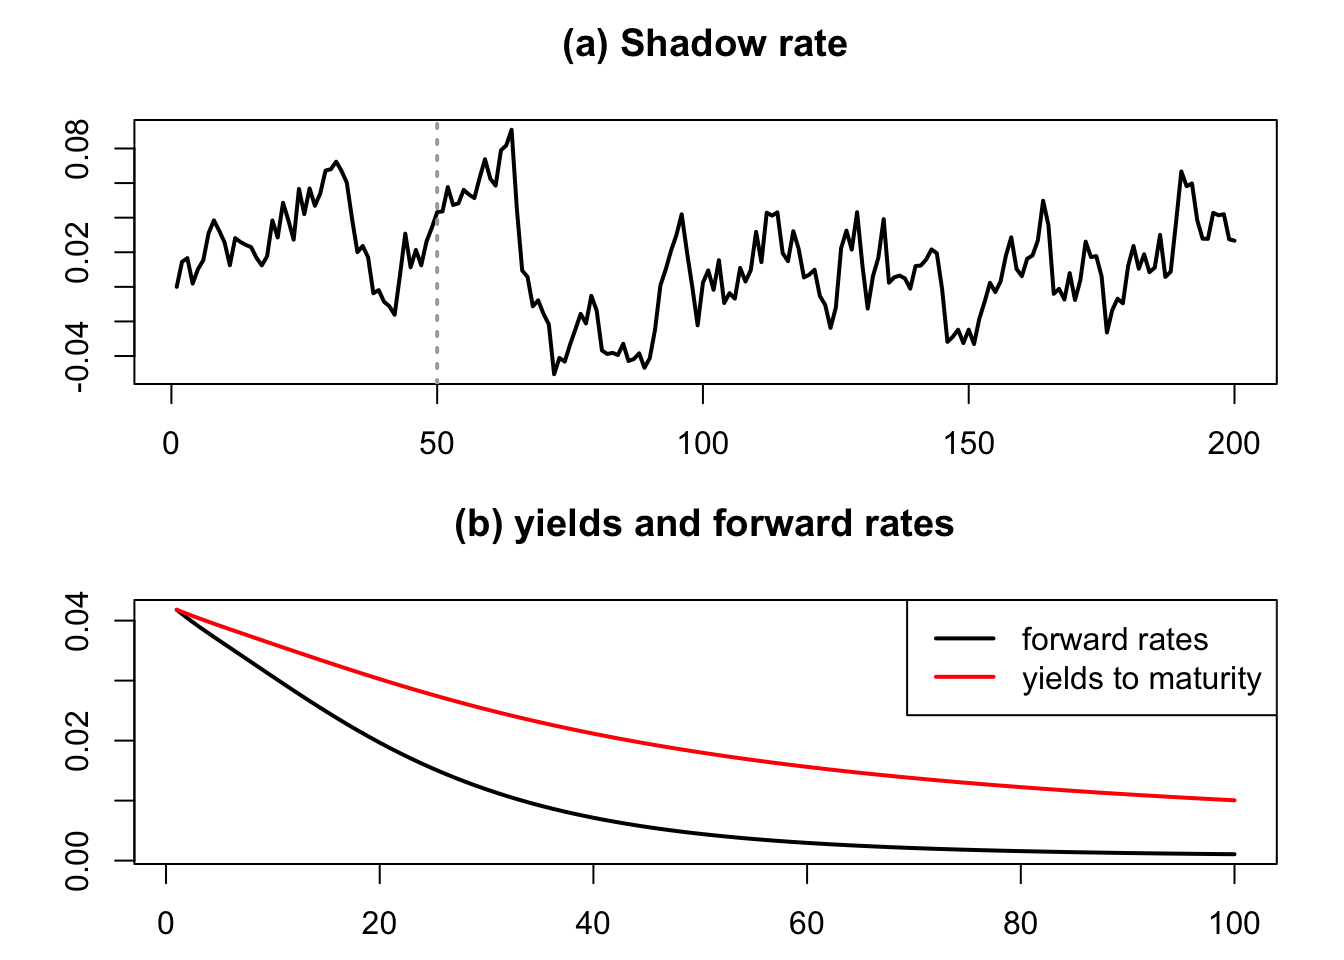
\includegraphics[width=0.95\linewidth]{TSM_files/figure-latex/WuXia-1} 

}

\caption{bla bla bla.}\label{fig:WuXia}
\end{figure}

\hypertarget{the-auto-regressive-gamma-approach}{%
\subsection{The auto-regressive gamma approach}\label{the-auto-regressive-gamma-approach}}

\citet{zarg_2017} introduce an affine framework where the short-term rate can stay at zero for a prolonged period of time and with a stochastic lift-off probability.

Under \(\mathbb{P}\) and \(\mathbb{Q}\), the state vector \(w_t\) follows a multi-variate auto-regressive gamma (VARG) process---a multivariate extension of Example \ref{exm:ARG1}. Conditionally on \(\underline{w_t}\), the \(n\) components of \(w_{t+1}\) are independent and distributed as follows:
\begin{equation}
\frac{w_{i,t+1}}{\mu_i} \sim \gamma(\nu_i+z_{i,t}) \quad \mbox{where} \quad z_{i,t} \sim {\mathcal P} \left( \alpha_i + \beta_i' w_t \right).\label{eq:VARG}
\end{equation}
If \(\mu = (\mu_1,\dots,\mu_n)'\), \(\alpha = (\alpha_1,\dots,\alpha_n)'\), \(\nu = (\nu_1,\dots,\nu_n)'\) and \(\beta = (\beta_1,\dots,\beta_n)\), then
\begin{eqnarray*}
\varphi_t(u) &=& \exp\left[\left(\frac{u \odot \mu}{1 - u \odot \mu}\right)'\beta' w_t \right.\\
&& \left. + \alpha'\left(\frac{u \odot \mu}{1 - u \odot \mu}\right) - \nu'\log(1 - u \odot \mu)\right],
\end{eqnarray*}
where \(\odot\) denotes the element-by-element multiplication and, where, with abuse of notation, the division and log operators work element-by-element when applied to vectors.

In their baseline model, \citet{zarg_2017} use four factors. They set \(\nu_1 = \nu_2 = 0\), implying that \(w_{1,t}\) and \(w_{2,t}\) can stay at zero (see Example \ref{exm:ARG1}). The short-term rate \(r_t\) is posited to be an affine combination of \(w_{1,t}\) and \(w_{2,t}\), that is:
\[
r_t = \omega'w_t = \omega_{1} w_{1,t} + \omega_{2} w_{2,t},
\]
hence, it can stay at zero.

Factors \(w_{3,t}\) and \(w_{4,t}\) Granger-cause \(w_{1,t}\) and \(w_{2,t}\), thereby causing \(r_t\). As a result, for \(h \ge 2\), \(R(t,h)\) is a non-zero combination of the four components of \(w_t\).

For the same reason, when \(r_t=0\), the lift-off probability depends on \(w_{3,t}\) and \(w_{4,t}\). The framework offers closed-form solutions for lift-off probabilities. Indeed, using Lemma \ref{lemma:mass}:
\[
\mathbb{P}_t(\alpha'w_{t+h}=0) = \lim_{u \rightarrow -\infty} \varphi_{t,h}(0,\dots,0,u\alpha),
\]
where \(\varphi_{t,h}\) is the multi-horizon Laplace transform defined in Eq. \eqref{eq:multiLT}, which can be computed using Proposition \ref{prp:reverseMLT}. We have:
\begin{equation}
\left\{
\begin{array}{l}
\mathbb{P}_t(r_{t+h}>0) = 1 - \lim_{u \rightarrow -\infty} \varphi_{t,h}(0,\dots,0,u\omega) \\ \\
\mathbb{P}_t(r_{t+1}=0,\dots,r_{t+h}=0) = \lim_{u \rightarrow -\infty} \varphi_{t,h}(u\omega,\dots,u\omega,u\omega) \equiv p_{h}\\ \\
\mathbb{P}_t(r_{t+1}=0,\dots,r_{t+h-1}=0,r_{t+h}>0) = p_{h-1} - p_h.
\end{array}
\right.
\end{equation}
Other lift-off probabilities, of the type \(\mathbb{P}_t[R(t+h,k)>threshold]\), can be derived from Eq. \eqref{eq:DPS}.

\citet{zarg_2017} esitmate this model by means of Kalman filtering techniques (see Subsection \ref{EstimationKF}). Observed variables include (levels of) yields, as well as survey-based forecasts of yields (see Subsection \ref{EstimationPersistency} and (e-GARCH-based) proxies of conditional variances (see Eq. \eqref{eq:condvar}).

\begin{figure}

{\centering 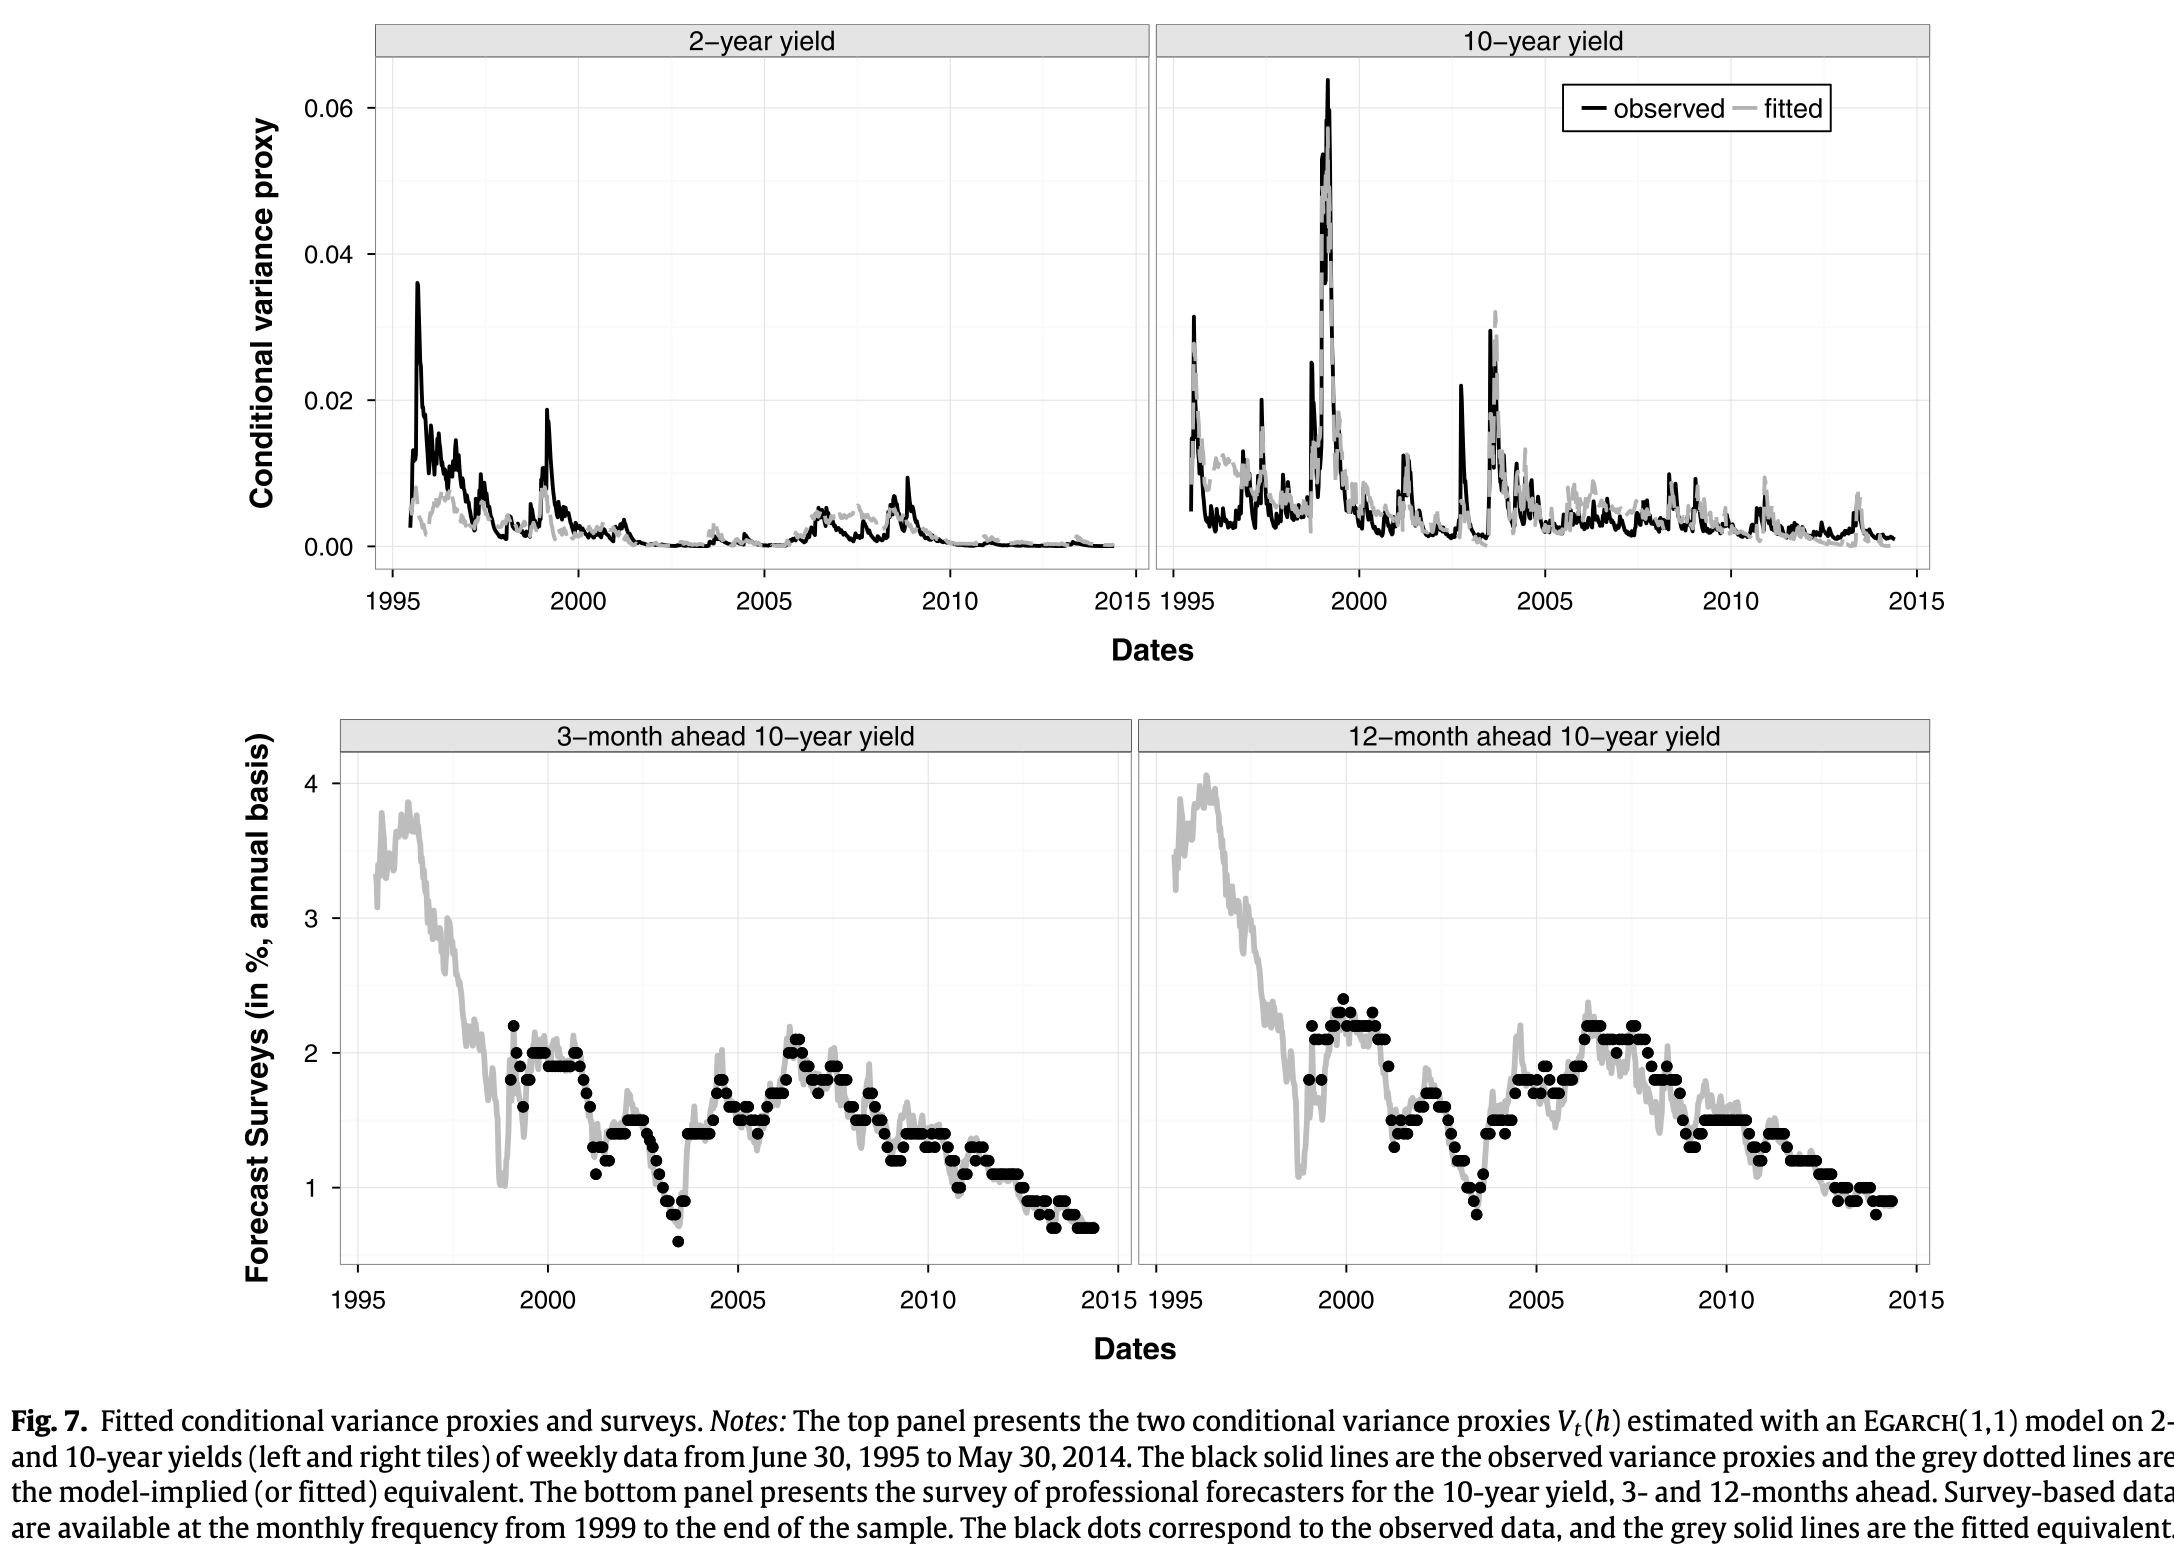
\includegraphics[width=0.95\linewidth]{figures/Figure_fit_ZARG} 

}

\caption{Source: Monfort et al. (2017). Model fit of conditional variances and surveys of professional forecasters.}\label{fig:fitZarg}
\end{figure}

\begin{figure}

{\centering 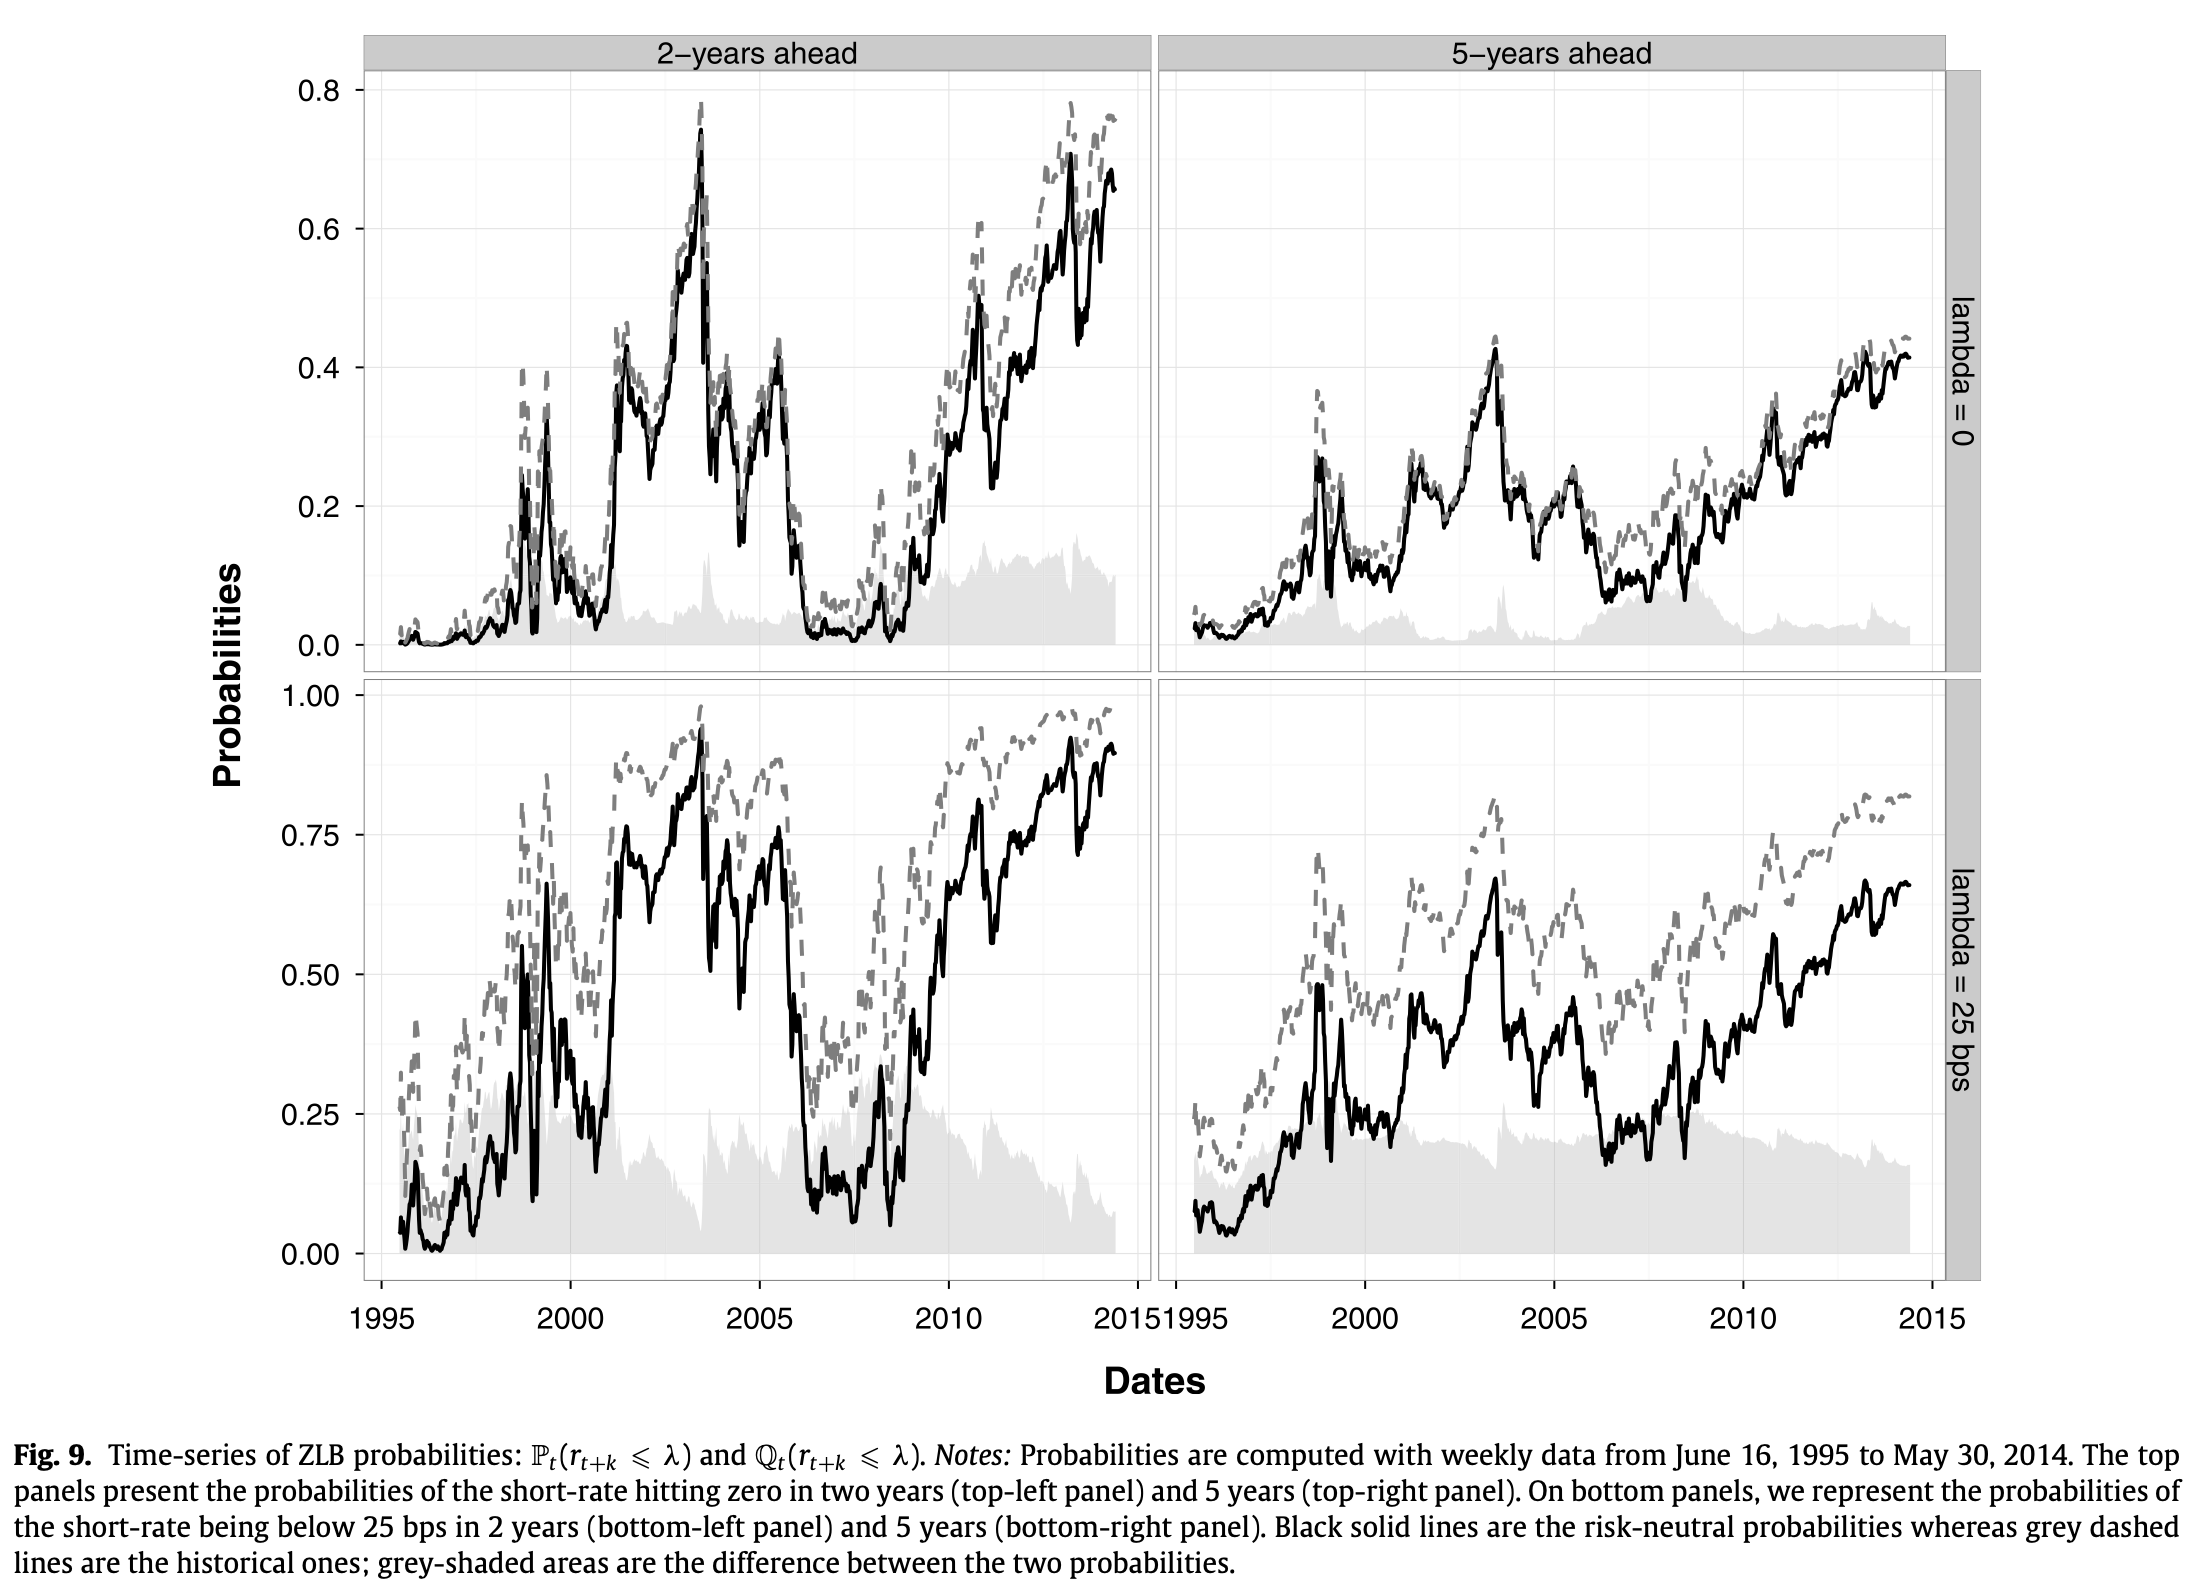
\includegraphics[width=0.95\linewidth]{figures/Figure_LiftOff} 

}

\caption{Source: Monfort et al. (2017). Lift-off probabilities.}\label{fig:liftOff}
\end{figure}

\hypertarget{references}{%
\chapter{References}\label{references}}

  \bibliography{book.bib,packages.bib}

\end{document}
